\documentclass[oneside,letterpaper]{memoir}

\usepackage{citthesis}

\usepackage[T1]{fontenc}
% Load lmodern for bold \ttfamily
\usepackage[]{lmodern}
%\usepackage[lighttt]{lmodern}
%\usepackage[bitstream-charter]{mathdesign}
%\usepackage[urw-garamond]{mathdesign}
\usepackage[sc]{mathpazo}
%\usepackage{fourier}
%\usepackage{lmodern}

\usepackage{stmaryrd}
\usepackage{graphicx}

\usepackage[colorlinks,linkcolor=blue,filecolor=blue,citecolor=blue,urlcolor=blue,backref=page]{hyperref}

%\usepackage{caption}
%\let\subcaption\undefined
%\let\subfloat\undefined
\newsubfloat{figure}

%Todd added for fractions
\usepackage{xfrac}
%Todd added this for strikeout \sout{}
\usepackage[normalem]{ulem}
%Todd added this for the reference to essence.sv.cmu.edu
\usepackage{hyperref}
%Todd added this to fix tables with an H
\usepackage{float}
%for no orphan lines
\usepackage[all]{nowidow}
 %for lableling a table as a figure
\usepackage{caption}

%Todd's commands
\newcommand{\strikeout}[1]{\sout{#1}}
\newcommand{\quotes}[1]{``#1''}
\newcommand{\participantQuote}[1]{\textit{``#1''}}
\newcommand{\singleQuote}[1]{`#1'}
\newcommand{\emphasis}[1]{\emph{#1}}
\newcommand{\ignore}[1]{}

\newcommand{\oneColumnWidth}{3.4in}
\newcommand{\twoColumnWidth}{7.1in}



\setauthor{Todd Sedano}
\settitle{Empirical Study of Iterative Software Development in Academia and Industry: Effectiveness, Optimization, and Extension of the Essence Kernel}
\doctors
\setchair{Dr.\ David Brumley}
\setdept{Electrical and Computer Engineering}
\setdegrees{B.S., Computer Science, Millersville University\\
M.S., Information Security, Carnegie Mellon University}
\setdefdate{May 2014}
\setgraddate{May 2014}
\setcopyyear{2014}

\begin{document}

\frontmatter

\thetitlepage
\copyrightpage

\section*{Acknowledgements}
Thanks!

\newpage
\section*{Abstract}
Software development continues to be a complex endeavor involving many disciplines and skill sets. Practitioners and researchers experiment, research, and adopt practices to simplify, understand, and create effective processes. 

Given the plethora of practices and methods, the Software Engineering Method and Theory (SEMAT) community created the Essence kernel as a unifying framework for describing and analyzing software engineering endeavors. 

My research goal is to evaluate the Essence kernel for practical use on academic and industrial software development projects, identify issues, and research solutions grounded in empirical evidence. 

At Carnegie Mellon University in Silicon Valley, I conducted a field study with masters of science in software engineering students as they completed team-based capstone projects using the Essence kernel. During weekly Essence Reflection meetings, the Essence kernel checklists helped students identify relevant goals to achieve, which enabled the team to steer the project to higher states. The student teams found value during project inception. However, teams found less value during the construction phase of iterative projects, as the Essence kernel offered few new goals hence loosing its ability to help the team steer the project. The original Essence kernel is method agnostic and does not directly support iterative development. Since most of agile software development occurs via iterative software development, adapting the Essence kernel to have goals for an iterative construction phase would increase its value to software development teams.

Following these results in academia, my objective is to continue my research in industry, with a focus on the practices at Pivotal. One of my next goals is to generate a process model that accurately describes iterative software projects at Pivotal. My plan is to conduct participant-observation of several software development projects at Pivotal. I will interview many software engineers and product managers to collect additional data. I'll iterate my research by incorporating this feedback. My expected result is a process model grounded in empirical data that supports iterative software development. 

\newpage
\tableofcontents
\listoffigures
\listoftables

\mainmatter


%%
%% Start line numbering here if you want
%%
%%\linenumbers

%note that import will do a clearfix
% \chapter{Essence Reflection Meetings}
\section{Abstract}

This paper presents an empirical evaluation of the team reflection support provided by the Software Engineering Method and Theory (SEMAT) Essence framework, and compares Essence reflection meetings to other types of team reflection meetings. The researchers conducted a field study involving seven graduate master student teams running Essence reflection meetings throughout their practicum projects aiming at delivering a working product for an industry client. The main result validates that Essence meetings generate reflective team discussions through a thinking framework that is holistic, state-based, goal- driven, and method-agnostic. Student teams benefit from stepping back and assessing the project holistically throughout its lifecycle. The goals set by the framework's checklists lead the teams to address critical aspects of the project that have not been considered. All team members are encouraged to express their views and influence the various project dimensions. Essence reflection meetings are comparable and complementary to Agile retrospectives, and project teams might want to leverage both techniques. The value added by Essence reflections is to surface unknown issues, help monitor progress, steer the project to a higher state, and prevent retrospectives from being repetitive by varying styles.

\section{Introduction}

The authors investigated a novel approach to monitoring and steering software development projects provided by the Software Engineering Method and Theory (SEMAT) Essence framework \cite{SEMATKernel}. Among the various benefits, team reflection stands out as being the most appreciated aspect of the approach from a student point of view. Therefore this paper elaborates on this result by focusing specifically on Essence team reflection.

There exists different types of reflection meetings. Some, like post-mortems or project retrospectives, are conducted once at the end of the project (or release). Others, like Agile retrospectives, are conducted throughout the project lifecycle, typically at the end of each iteration or Sprint. There are many variations or styles of Agile retrospectives \cite{Derby2006, KuaRetrospectiveHandbook}, and different authors refer to them using different names, including iteration retrospectives, Sprint retrospectives, or heartbeat retrospectives. In this paper we explain why Essence reflection meetings are comparable to Agile retrospectives, highlight the similarities and differences between the two, and suggest how project teams could leverage both techniques in a complementary fashion.

This paper introduces the SEMAT's Essence framework, presents the field study, and reports on the field study results with a focus on team reflection.

\section{SEMAT Essence Overview}
The core idea of the Software Engineering Method and Theory (SEMAT) Essence framework \cite{SEMATKernel} is that software projects exhibit universal behavior and transition through identifiable states as they progress. The states are grouped by software engineering dimensions called \quotes{alphas.} Essence identifies seven alphas as core to every software engineering project: \textbf{Stakeholders}, \textbf{Opportunity}, \textbf{Requirements}, \textbf{Software System}, \textbf{Team}, \textbf{Way of Working}, and \textbf{Work}. These seven alphas serve as the Essence kernel. Each alpha progresses through a number of states during the project lifecycle. For example, the \textbf{Stakeholders} alpha progresses through the states \textit{Recognized}, \textit{Represented}, \textit{Involved}, \textit{In Agreement}, \textit{Satisfied for Deployment}, and \textit{Satisfied in Use}. Each state includes a checklist to help determine if the project has achieved that state or not. Table \ref{EssenceReflectionMeetings} shows the checklist related to the Bounded state of the \textbf{Requirements} alpha.




\section{Field Study Description}
The field study aims at evaluating the effectiveness of the SEMAT Essence's approach. A complete description is available in \cite{ICSE2014}. The study includes seven student teams: three geographically distributed student teams and four co-located student teams. Each team worked on creating or evolving a software solution for a different industry client, like an electric car fleet management system or a survivable social network. By design, the projects had a medium to high level of technical complexity, as they often involved multiple technologies or platforms or integrate with legacy systems. The practicum projects ran for 12 to 15 weeks, during which each student dedicated about 20 hours per week to the project. Students worked in teams of two to five members. Teams determined their own software development approach. Most students had a reasonable knowledge of a diverse set of generally accepted software engineering practices, and the ability to execute these practices somehow effectively. All projects adopted an iterative lifecycle.
   
The teams were asked to leverage Essence throughout their project. Each team met on a regular basis (mostly weekly) for a 30 minutes Essence session. During each session, the team covered most or all of the alphas. For each alpha, the team identified their project current state, target state, and any work items necessary to transition from the current to the target state. In order to avoid anchoring bias, the current state identification was performed using a \quotes{poker game} approach \cite{ICSE2014}. In that context, each participant secretly determines the current state and all reveal their current state at the same time. In case of disagreement, the team discusses the different points of view until the participants reach an agreement. Table \ref{EssenceReflectionMeetings} provides a conceptual representation of how Essence was used in practice by each team.

A faculty member was present to facilitate each session. Faculty involvement was kept to a minimum to limit influencing the students. The faculty's role was constrained to recording progress, guiding the team through the application of the approach, and validating the objectivity of the team's self-assessment of their project state. At the end of each project a survey was sent to the students to collect their feedback on the application of the approach.

The qualitative and quantitative value of Essence refection meetings was measured primarily based on students' feedback collected during the weekly meetings and final survey.

\section{Field Study Results}
\textbf{Research Question:} How does Essence support team reflection?

The original intent of each Essence session was to monitor the team's progress and steer the project towards higher Essence states. The sessions also provided a natural setting for team reflection. Indeed, a majority of students (72\%) spontaneously mentioned reflection or retrospectives in the survey responses (80\% of the students participated in the survey).

For instance, one student mentioned: \participantQuote{What I liked most about Essence is that it invoked reflective discussion.} Another student mentioned: \participantQuote{The team was pleased to see that Essence also covered `The Way of Working' as well as `The Team'. These two topics generated useful team introspection at the beginning of the practicum and were nice reminders that the team does constant checkups for the overall condition of the members and the project.} Overall, the survey responses touch upon the following key ingredients of Essence reflection meetings:

\textbf{Holistic Thinking Framework}. The seven alphas, together with their states and checklists, provide the team with a thinking framework encouraging the team to think about the project in a holistic fashion, based on seven project dimensions (a.k.a. alphas). One student noted: \participantQuote{Essence enabled the team to keep an eye on the status of the project by zooming out and assessing the overall picture.} Stepping back and looking at the project holistically provides the distance and perspectives needed to understand a situation, reflect, and make informed decisions.

\textbf{State-based \& Goal-driven Thinking Framework}. The Essence thinking framework evolves throughout the project lifecycle, based on the project's specific alpha states. At each state, new checklist items (goals) are presented to the team, encouraging the team members to think about and address aspects of the project that are relevant to the current state. One student noted: \participantQuote{I like the fact that Essence provides a structured way of thinking about critical aspects of the project at different stages of the project.}

\textbf{Team Discussion}. Essence reflection meetings enable all team members to express their views and influence the different aspects of the project. Here is an illustrating quote: \participantQuote{Essence meetings allowed everyone on the team to have a say in the different aspects of the project.} Another student added: \participantQuote{It allows us to reflect on where we stand in the project and remind us of the points we are missing.}

\begin{figure}[t]
\centering
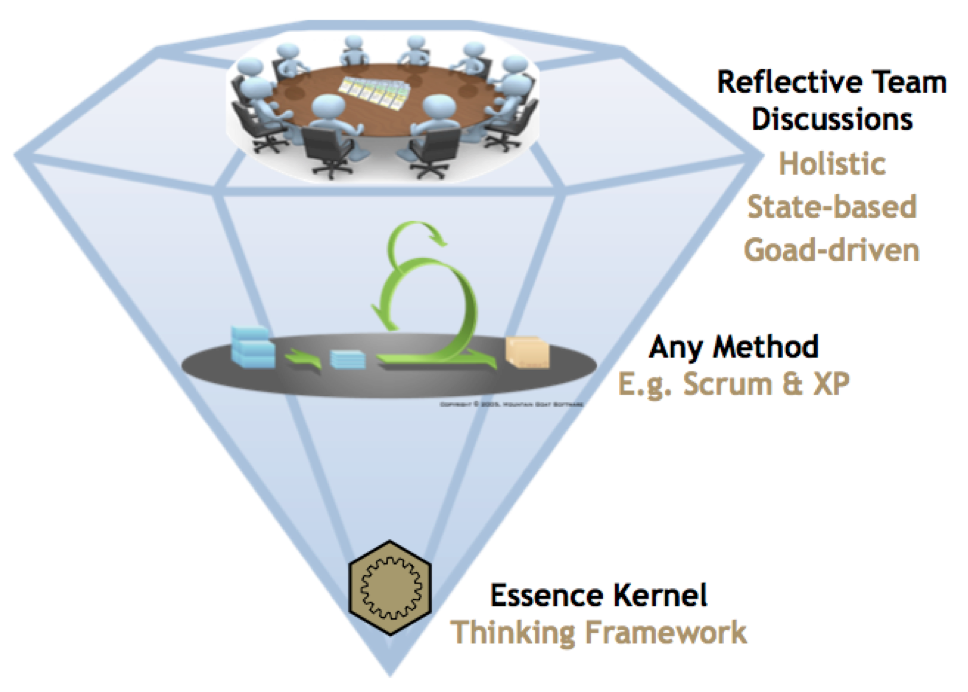
\includegraphics[width=3.4in]{reflection_meeting_images/EssenceDiamondEffect.png}
\caption{ Essence kernel's diamond effect}
\label{EssenceDiamondEffect}
\end{figure}

\textbf{Method-Agnostic}. The team decides what to do to reach the goals set by the target states. The team has the flexibility to leverage any software development method or set of practices that best suit their needs. This is illustrated in Figure \ref{EssenceDiamondEffect} with the Essence kernel's \quotes{diamond effect,} where the kernel alphas \quotes{radiate} to enable reflective discussions touching the many facets of the project throughout its lifecycle, independently of the software development method adopted by the team.

In conclusion, Essence supports team reflection by generating reflective team discussions through a thinking framework that is holistic, state-based, goal-driven, and method-agnostic. The teams benefit from stepping back and assessing the project holistically throughout its lifecycle. The goals set by the alpha state checklists lead the team to address critical aspects of the project that have been neglected. These aspects go beyond technology by including elements like \textbf{Team}, \textbf{Way of Working}, or \textbf{Stakeholders}.

\textbf{Research Question}: How does Essence reflection meetings compare to other types of reflection meetings?

Essence reflection meetings follow a state-based approach, with states covering the entire project lifecycle. Consequently, Essence reflection meetings are most effective if conducted on a regular basis throughout the entire project lifecycle. Therefore, Essence reflection meetings are not comparable to post-mortems or project retrospectives that are conducted only once at the end of the project (or release). Essence reflection meetings could be compared to Agile retrospectives \cite{Derby2006, KuaRetrospectiveHandbook}, because they are also conducted throughout the project lifecycle, typically at the end of each iteration or Sprint.

In this section we are comparing Agile retrospectives and Essence reflection meetings in terms of purpose, frequency, duration, structure, content, outcome, and facilitation concerns.

\textbf{Purpose}. The goal of an Agile retrospective is for the team to contemplate what worked and did not work during the last iteration in order to adapt the methods and teamwork moving forward. The focus is mostly on the past. The goal of an Essence reflection is for the team to consider various project dimensions in order to bring the whole project towards a higher state. The focus is mostly on the future.
  
\textbf{Frequency}. Both Agile retrospectives and Essence reflections can be conducted at the end of an iteration or Sprint, or at other intervals defined by the project team. During our field study, each team generally met on a weekly basis. We recommend frequent sessions early in the project when many issues arise. Later on, once a team becomes a high-performing team producing high quality outcome, the team needs less support and the frequency of the sessions could decrease.

\textbf{Duration}. Both Agile retrospectives and Essence reflections can be time boxed to a short session ranging from 30 minutes to a few hours. During our field study, each team generally met for a 30- minute session. We recommend adjusting the duration based on the team size and any other known parameters that might influence the length of the conversations, like team dynamic, issues and uncertainty, or session frequency.

\textbf{Structure}. While facilitators may run Agile retrospectives differently, many adopt a structure similar to the one proposed by Derby and Larsen in \cite{Derby2006}. Derby and Larsen generalize the stages of Agile retrospectives as: (1) Set the stage, (2) Gather data, (3) Generate insights, (4) Decide what to do, and (5) Close the retrospective. Even though Agile retrospectives and Essence reflections have a different structure, there are some similarities. During an Essence reflection meeting, the team repeats the key steps of gathering of data, generation of insights, and deciding what to do for each alpha. With the Essence kernel's seven alphas, this produces seven focused passes through the Agile retrospective stages. This structure is illustrated in Table \ref{ReflectionMeetingStructure}.

\begin{table}[t]
\renewcommand{\arraystretch}{1.5}
\centering
\caption{Essence reflection meeting structure}
\label{ReflectionMeetingStructure}
\begin{tabular}{p{3in}}
\hline
\textbf{Set the stage} (done informally) \\
\textit{For each alpha}:
  \begin{itemize}
  \item \textbf{Gather data (alpha states)} 
  
   Discuss alpha-related work since last session
   and agree on current and target states
  
  \item \textbf{Generate insights}

  Understand \textit{why} the target state is not achieved
  
  \item \textbf{Decide what to do}
  
  Set some goals to reach the target state 
  and agree on how to reach the goals

  \end{itemize}
    
\textbf{Close the retrospective} (done informally) \\
\hline
\end{tabular}
\end{table}


\textbf{Content}. One difference between Agile retrospectives and Essence reflections relates to the elicitation of topics to be covered during a session. During Agile retrospectives the topics discussed are elicited by the participants, while during Essence reflections the topics are determined by the alphas and their corresponding checklists. Issues emerge once the related alphas are covered. As a consequence, Agile retrospectives tend to focus on known issues while Essence reflections tend to make unknown issues apparent by covering the project holistically and reminding participants of \participantQuote{critical areas that are sometimes neglected.}

\textbf{Outcome}. Both Agile retrospectives and Essence reflections result in a small number of work items to be addressed, ideally before the next session. During an Agile retrospective, participants typically generate many possible work items that are prioritized and then limited to a few high value items to be addressed during the next iteration. During our field study, an average of 5 work items were generated per session. The identified work items were added to the team's work item list or backlog, and fed into the next planning activity when applicable.

\textbf{Facilitation}. Both Agile retrospectives and Essence reflections benefit from being conducted by an experienced and neutral facilitator. While this is often recommended for Agile retrospectives \cite{KuaRetrospectiveHandbook}, the need for a facilitator is reduced with Essence reflections as the Essence alphas and their checklists guide the discussions. A facilitator is only required during the initial sessions for training purposes. Similarly, it is generally recommended to prepare for Agile retrospectives ahead of time \cite{Derby2006, KuaRetrospectiveHandbook}. Essence reflection meetings might require the facilitator to print the cards ahead of time. We are currently leveraging an open source tool (available at http://essence.sv.cmu.edu) developed internally that provides digital cards, hence freeing us from any preparation. With such a tool, Essence reflection meetings are conducted very effectively with geographically distributed teams.

In conclusion, Essence reflection meetings could be compared to Agile retrospectives. Despite similarities between the two approaches, there are some key differences in terms of purpose and content. While Agile retrospectives aim at inspecting the last iteration in order to adapt the methods and teamwork (with a focus on the past), Essence reflections aim at considering various project dimensions in order to bring the whole project towards a higher state (with a focus on the future). While most styles of Agile retrospectives tend to focus on known issues, Essence reflections tend to make unknown issues apparent by covering the project holistically and reminding participants of critical areas that might be overlooked. These differences make Essence reflections and Agile retrospectives complementary. This is illustrated by the following student quote: \participantQuote{Though the team was holding retrospectives every week already, having Essence discussions be a part of it allowed the team to touch on important aspects of the project; aspects which would otherwise be ignored.}

\section {Conclusion}
Essence reflections are valuable and complementary to Agile retrospectives. Facilitators and project teams might want to leverage both. For instance, one might decide to conduct regular Essence reflection meetings during project initiation when the monitoring and steering mechanisms are the most effective \cite{ICSE2014}, then alternate between Essence reflections and other styles of Agile retrospectives. The value added by Essence reflections is to surface unknown issues, help monitor and steer the project towards a higher state, and prevent retrospectives from being repetitive by varying styles.

The results presented in this paper are limited to Essence reflection meetings with a facilitator. More research is necessary to assess the meetings' effectiveness without facilitators. Following the field study, we have been observing eight additional practicum teams. Our observations are consistent with the ones presented in the paper. We continue to collect data to evaluate the SEMAT Essence's framework with a focus on both effectiveness of the approach and accuracy of the model.

\begin{table*}[t]
\caption{How Essence is used in practice by a student team}
\centering
\begin{tabular}{l|l}
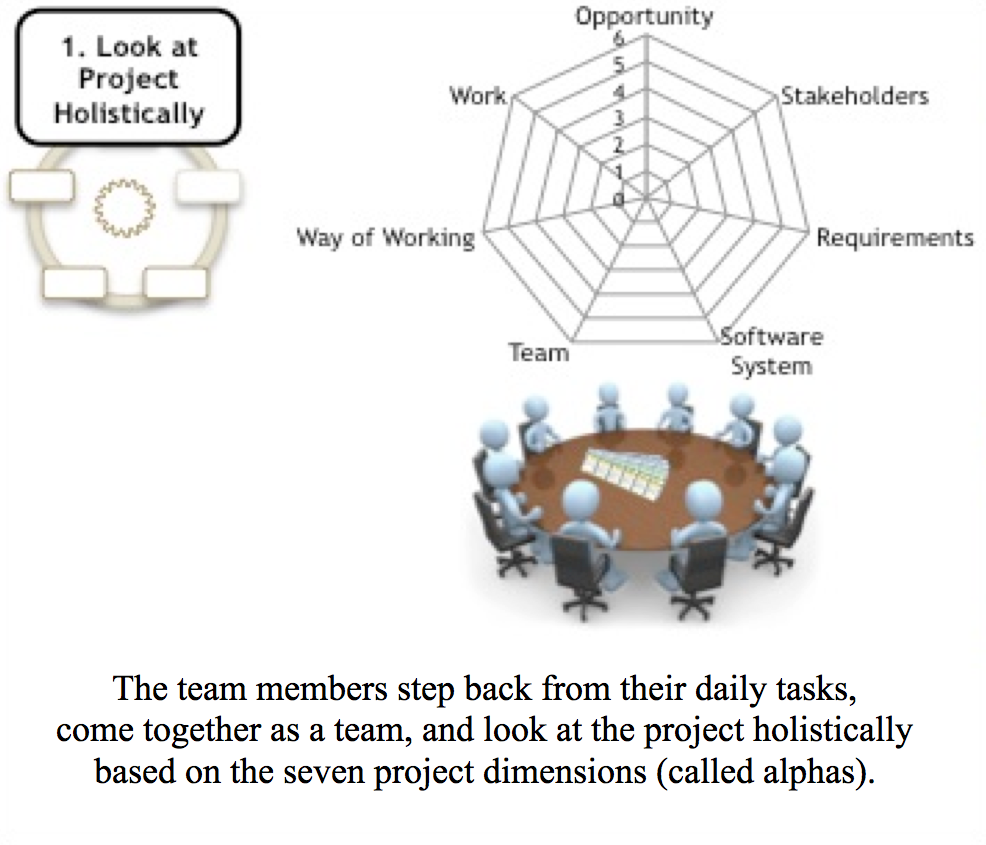
\includegraphics[width=3.2in]{reflection_meeting_images/EssenceMeetingStep1.png} & 
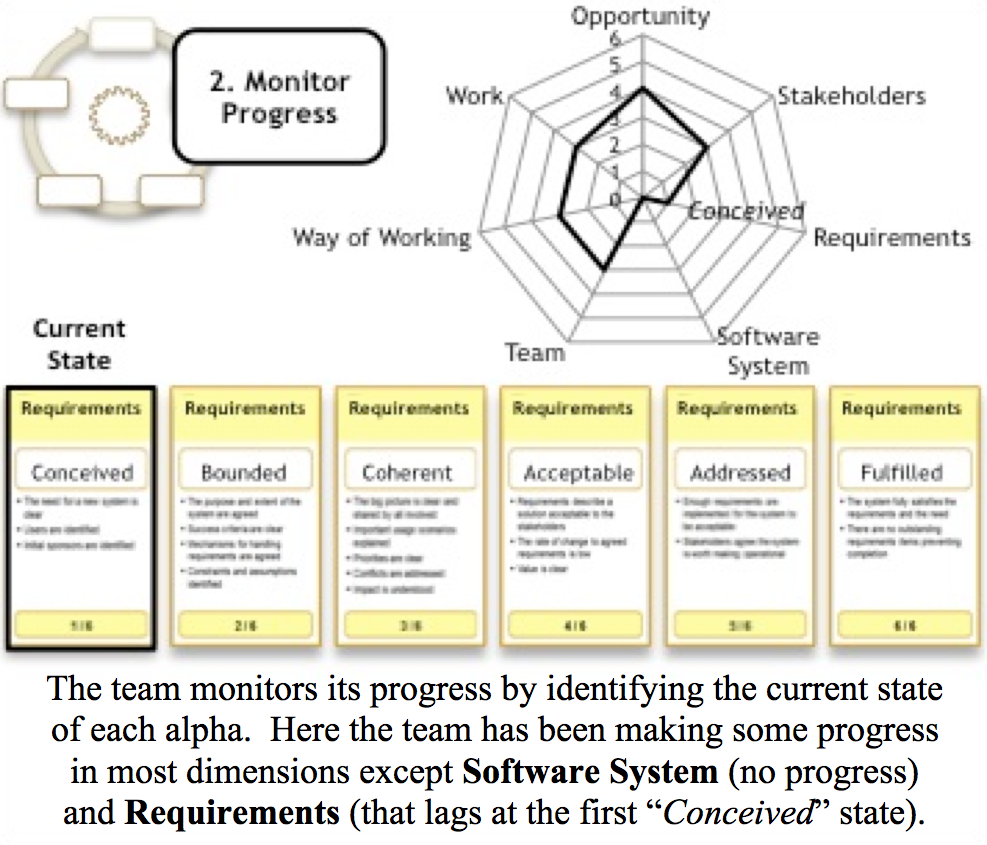
\includegraphics[width=3.2in]{reflection_meeting_images/EssenceMeetingStep2.png} \\
\hline
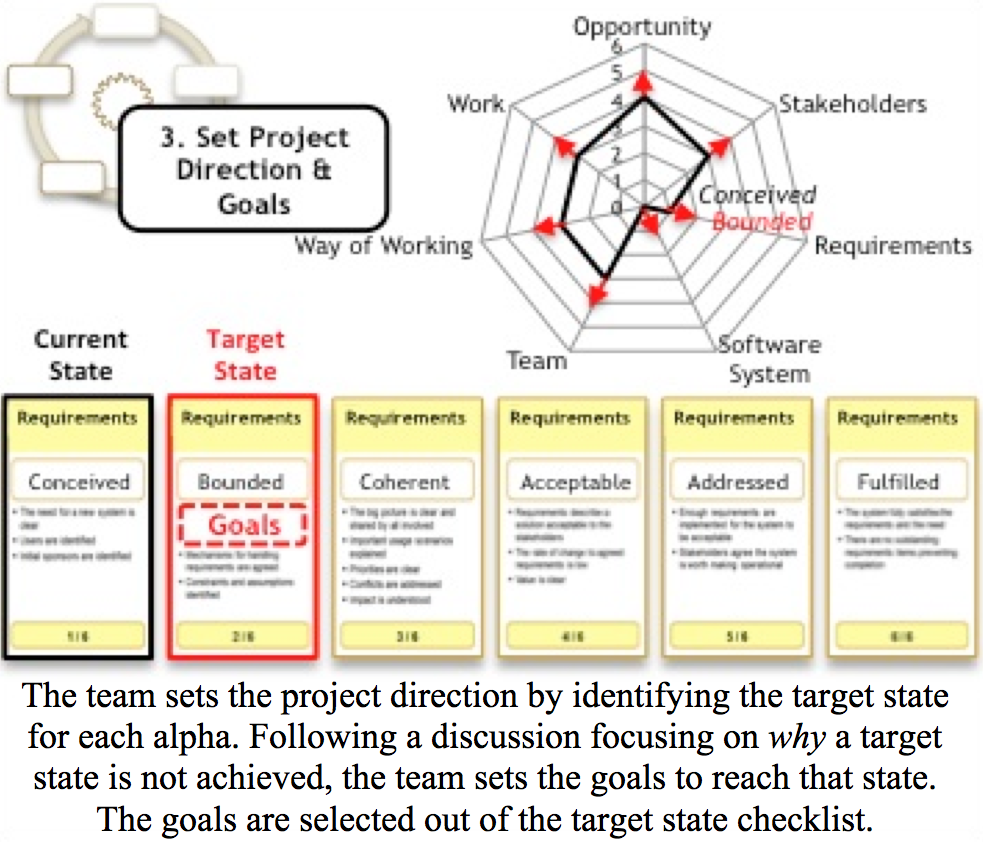
\includegraphics[width=3.2in]{reflection_meeting_images/EssenceMeetingStep3.png} &
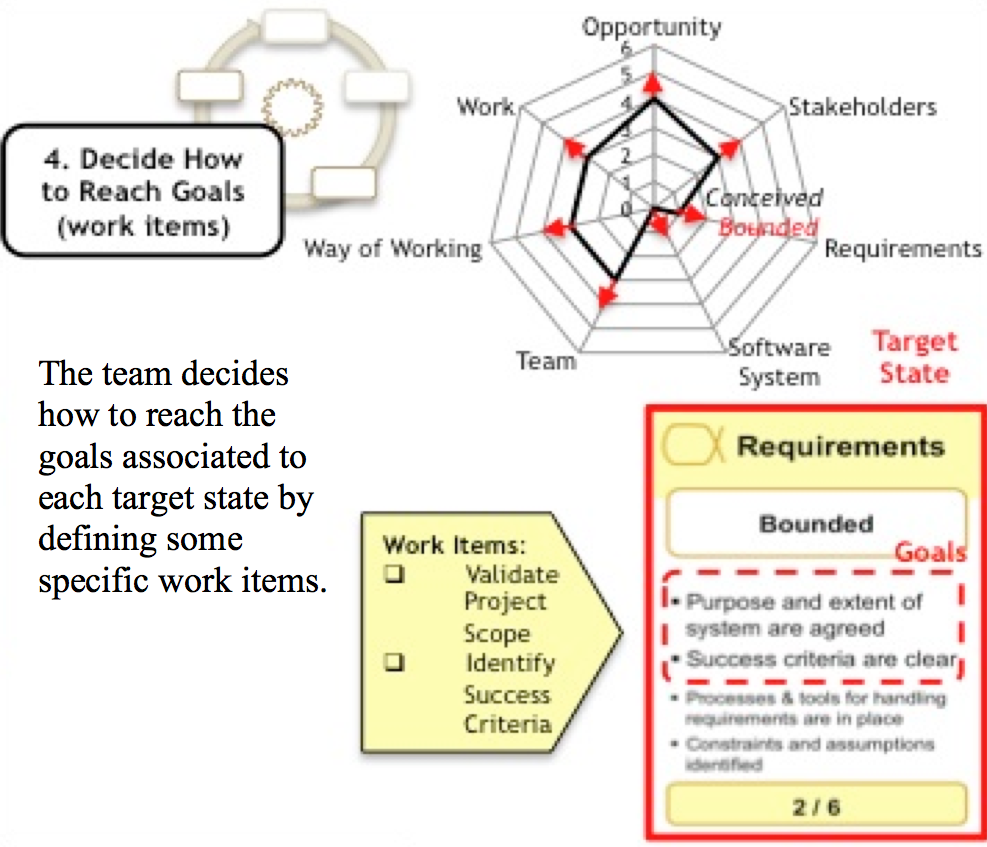
\includegraphics[width=3.2in]{reflection_meeting_images/EssenceMeetingStep4.png} \\
\hline
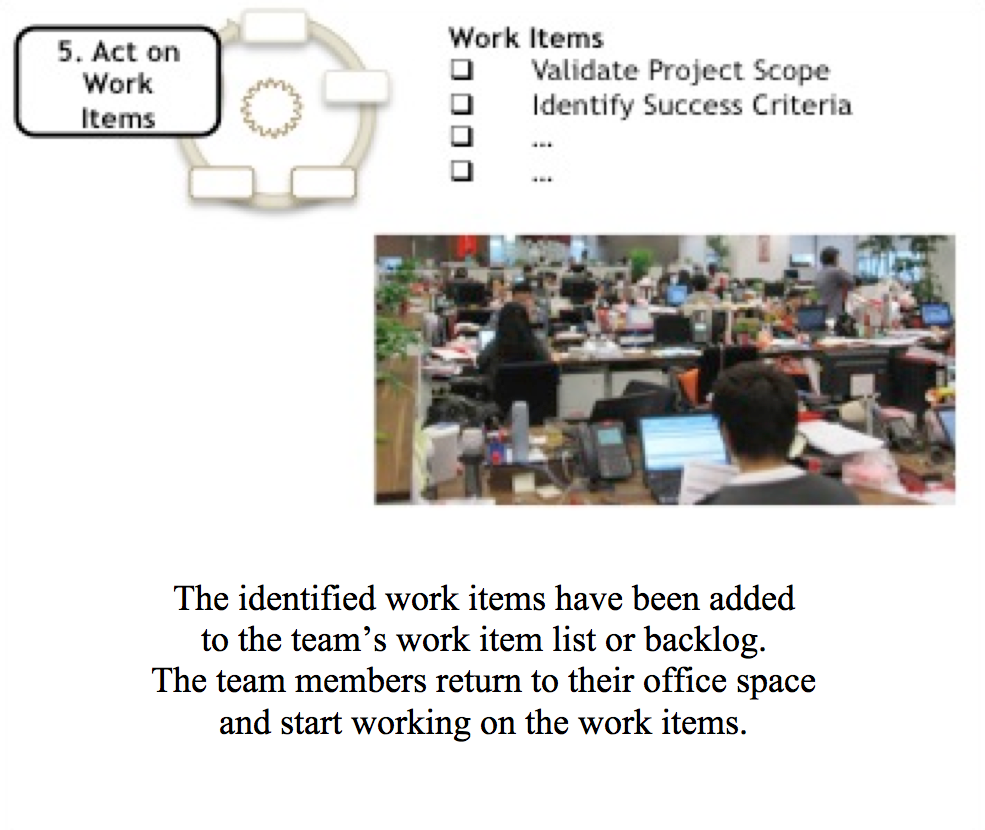
\includegraphics[width=3.2in]{reflection_meeting_images/EssenceMeetingStep5.png} &
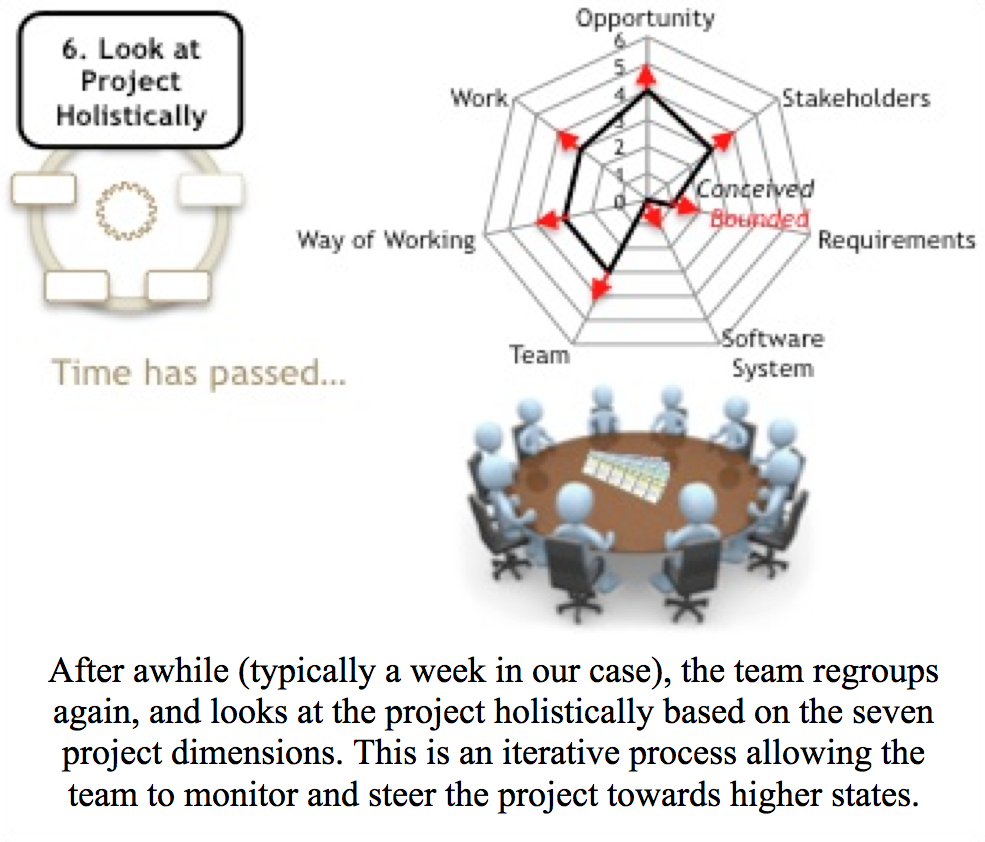
\includegraphics[width=3.2in]{reflection_meeting_images/EssenceMeetingStep6.png} \\
\end{tabular}
\label{EssenceReflectionMeetings}
\end{table*}
% \chapter{Essence Steering}
\section{Abstract}
At Carnegie Mellon University in Silicon Valley, the graduate master program ends with a practicum project during which students serve as software engineering consultants for an industry client. In this context, students are challenged to demonstrate their ability to work on self-managing and self-organizing teams. This paper presents a field study of the Software Engineering Method and Theory (SEMAT) Essence framework. The objective is to evaluate the effectiveness of the Essence's novel state-based monitoring and goal-driven steering approach provided by the Essence kernel alphas and their states. The researchers conducted the study on seven graduate master student teams applying the approach throughout their practicum projects. The research methodology involves weekly observation and recording of each team's state progression and collecting students' reflection on the application of the approach. The main result validates that the approach provides student teams with a holistic, lightweight, non-prescriptive and method-agnostic way to monitor progress and steer projects, as well as an effective structure for team reflection and risk management. The paper also validates that the Essence kernel provides an effective mechanism for monitoring and steering work common to most student software projects. This includes the work done during project initiation as well as the work done at the project or release level. Support for technical work should come from additional practices added on top of the kernel, or by extending or altering the kernel definition. The conclusion is that the approach enables students to learn to steer projects effectively by addressing the various dimensions of software engineering. Hence the approach could be leveraged in software engineering education.

\section{Introduction}

This paper presents the results of a field study of the Software Engineering Method and Theory (SEMAT) Essence framework \cite{SEMATKernel, EssenceBook} investigating the Essence kernels' novel approach to monitoring and steering software development projects. One of the promises of the approach lies in its potential ability to monitor any type of project holistically based on universal project states and steer these projects based on universal goals, hence making the monitoring and steering mechanisms independent from the method (such as Scrum \cite{AgileProjectManagement} and XP \cite{BeckExtremeProgramming2000}) or set of practices adopted by the project team.

We are interested in understanding the strengths and weaknesses of Essence by gaining experience of using the approach on real projects. We conducted a field study involving seven co-located and distributed student teams working on industrial projects. These students finish their graduate program with a project course at Carnegie Mellon University in Silicon Valley in the context of the Master of Science in Software Engineering program. During the project each student has the opportunity to apply the software engineering skills acquired throughout the program to solve a real industry problem. Monitoring and steering projects with the Essence kernel allows the researchers to identify where value is added for an educational program. Student team projects serve as a possible metaphor for newly formed industry team projects; the value added for a student team could transfer to an industry team.

As faculty, we allow teams to be self-organizing and responsible for their decisions, yet at the same time expect them to incorporate generally accepted software engineering practices, and demonstrate the ability to effectively steer their project. Each team manages its own project with minimal faculty supervision. In the past, the faculty observed that with minimal supervision some teams revert to old habits \cite{BareissTransferable}. As soon as the starting bell sounds, they can act as racetrack horses running towards the finish line with blinders, ignoring what they have learned in class and without concerns for software engineering discipline. The new freedom and the chance to write code for a client lead them to focus mostly on implementation and therefore to adopting a suboptimal way of working.

Our research hypothesis contends that Essence's monitoring and steering approach provides a lightweight framework for students to look at their project holistically, helping them to address various project dimensions beyond implementation. We stipulate that the framework acts as a routine reminder about applicable software engineering practices covered in previous courses, and this without being prescriptive and while being method agnostic. For instance, by using this technique, we expect students to think about involving stakeholders, improving the team's way of working, and demonstrating that the software system has the desired quality characteristics.

This paper reviews SEMAT's Essence framework and kernel, describes the field study planning and execution, reports on the analysis and interpretation of the field study data, recommends effective practices for introduction of Essence to a software engineering curriculum, and summarizes the conclusions.

\section{SEMAT ESSENCE OVERVIEW}
In 2009, Ivar Jacobson, Bertrand Meyer, and Richard Soley started work on the \quotes{Software Engineering Method and Theory} (SEMAT) with the goal of \quotes{re-founding software engineering as a rigorous discipline} \cite{JacobsonCallForAction}. While many software engineering principles, techniques, practices and methods exist, the SEMAT founders' ambition is to create a general theory of software engineering and a unifying process framework. Out of their initiative has emerged the SEMAT Essence language and kernel, which became an Object Management Group (OMG) beta standard in 2013.

The core idea of Essence is that software projects exhibit universal behavior and transition through identifiable states as they progress. Essence groups these states together by different software engineering aspects or dimensions called \quotes{alphas.} Essence identifies seven alphas as core to every software engineering project: \textbf{Stakeholders}, \textbf{Opportunity}, \textbf{Requirements}, \textbf{Software System}, \textbf{Team}, \textbf{Way of Working}, and \textbf{Work}. These seven alphas serve as the Essence kernel as illustrated in Figure \ref{EssenceKernel}.

\begin{figure}[h]
\centering
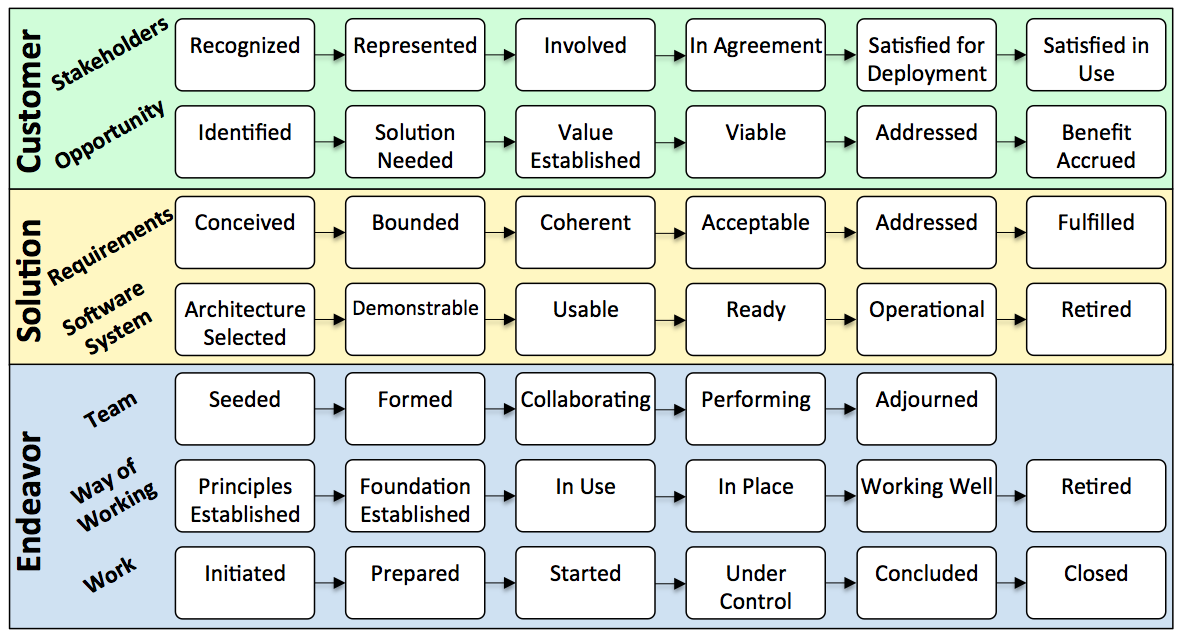
\includegraphics[width=3.30in]{project_steering_images/EssenceKernel.png}
\caption{Essence kernel alphas and their states }
\label{EssenceKernel}
\end{figure}

Each alpha progresses through a number of states during the project lifecycle. For example, the \textbf{Stakeholders} alpha progresses through the states \textit{Recognized}, \textit{Represented}, \textit{Involved}, \textit{In Agreement}, \textit{Satisfied for Deployment}, and \textit{Satisfied in Use}. Each state includes a checklist to help determine if the project has achieved that state. Each checklist item provides a goal to be reached in order to progress to that state.

Despite the sequential definition of the states for each alpha, in practice, projects could fall back to previous states. Similarly, in some circumstances, it might make sense for a project to achieve a number of states simultaneously within a given alpha.

The SEMAT vision is also to create a library of practices described using the Essence language and sitting on top of the Essence kernel. Practices would be composed to become specific methods addressing specific project or organization needs. Practices would help a team identify how to progress their project from one state to the next.

In The Essence of Software Engineering \cite{EssenceBook}, the authors identify three separate applications of Essence: 1) project monitoring and steering, 2) determining when to green light projects, and 3) describing workflow through an organizational structure. This paper focuses mostly on the first application, project monitoring and steering, where a team assesses its current project state in each of the alphas and identifies possible actions to help transition from the current state to the next target state.

\section{Field Study Description}
\label{Field Study Description}

The study focuses on understanding what value do project teams receive from following the SEMAT Essence's monitoring and steering approach provided by the kernel alphas and their states. Essence was introduced to master students at the beginning of their practicum projects. The students had no prior knowledge of Essence.

Using the goal template from GQM \cite{GQM}, our research goal is to:

\begin{table}[h]
\renewcommand{\arraystretch}{1.3}
\centering
\begin{tabular}{|p{1.20in}|p{1.90in}|}
\hline
\textbf{Analyze} & SEMAT Essence's monitoring and steering approach provided by the kernel alphas and their states \\ \hline
\textbf{for the purpose of} & evaluation \\ \hline
\textbf{with respect to its} & effectiveness \\ \hline
\textbf{from the point of view of the} & project team, educator, and researcher \\ \hline
\textbf{in the context of} & the software engineering practicum graduate course at Carnegie Mellon University. \\
\hline
\end{tabular}
\end{table}
 
This paper decomposes this goal into the following questions:

\textbf{Research Question 1}: Does the SEMAT Essence's monitoring and steering approach provide value to the project team?

\textbf{Research Question 2}: How does the approach provide value to the project team?

\textbf{Research Question 3}: When in the project lifecycle does the approach add value?

\textbf{Research Question 4}: What are the limitations to the approach's effectiveness?

The first section below describes the context of each project involved during the field study. The second section presents how Essence was introduced to the teams, either incrementally or using a workshop approach. The final section describes how the teams have been leveraging Essence during the remaining of their project.

\subsection{Practicum Projects' Context}


\begin{table*}[t]
\centering
\renewcommand{\arraystretch}{1.4}
\caption{Practicum projects' context}
\label{PracticumProjectsContext}
% \begin{tabular}{|p{0.6in}|p{1.1in}|p{1.1in}|}
\begin{tabular}{|p{0.75in}|p{1.05in}|p{0.3in}|p{1.05in}|p{0.7in}|p{2.3in}|}
\hline
\textbf{Team Name} &
\textbf{Industry Project} &
\textbf{Team Size} &
\textbf{Team Distribution} & 
\textbf{Average Work Experience} &
\textbf{Technical Complexity} \\
\hline
\hline
\multicolumn{6}{|l|}{\textbf{First Pilot Projects}} \\ 
\hline

Distributed-1 & 
Rendering of audio streams for accessibility purpose &
3 &
Distributed within same time zone &
10 years &
Integration with legacy code on a single platform involving C, HTML5 and open-source technology. \\
\hline

Distributed-2 & 
Access and preservation of electronic journals & 
4 & 
Distributed across 2 time zones & 
6 years &
Integration with legacy code on a single platform involving Java, MongoDB, Apache Jena and open-source technology. \\
 \hline

Distributed-3 & 
Survivable social network & 
4 & 
Distributed across 2 time zones & 
8 years &
Multi-platform involving Ruby on Rails, Javascript, jQuery Mobile. Embedded system constraints. \\
\hline

\multicolumn{6}{|l|}{\textbf{Second Pilot Projects}} \\ 
\hline

Co-located-1 & 
Electric vehicle fleet management & 
2 & 
Co-located & 
3 years & 
Green-field development involving Query, Node.js and MongoDB. Integration with Rest APIs for two vehicle brands. \\
\hline

Co-located-2 & 
Sonification of financial trading information & 
4 & 
Co-located & 
3 years & 
Integrates with third party APIs (Yahoo! and Google Finance). Involves Objective C, Ruby on Rails, iOS, Google App Engine and Python. Requires financial knowledge. Has a special focus on user experience. \\
\hline

Co-located-3 & 
Mobile performance testing & 
3 & 
Co-located & 
4 years & 
Xcode, Instruments, Eclipse, iOS 6.0, Android 4.2, jQuery Mobile, HTML5, Benchmark.js, Appception, Pivotal tracker, Redmine, GitHub, RubyMine, Rails 3.2, Ruby 1.9.2. Heroku, Amazon EC2, HighCharts.js, CSS3, Cordova \\
\hline

Co-located-4 & 
Virtual sensors definition and management & 
5 & 
Co-located & 
5 years & 
Multi-platforms involving HTML5, Javascript and j2ee. \\
\hline

\end{tabular}
\end{table*}


The authors introduced Essence to seven student teams: three geographically distributed student teams, referred as Distributed-1 to Distributed-3 for the purpose of this paper, and four co-located student teams, referred as Co-located-1 to Co-located-4. As shown in Table \ref{PracticumProjectsContext}, each team worked on creating or evolving a software solution for a different client, like an electric car fleet management system or a survivable social network. By design, the projects had a medium to high level of technical complexity, as they often involved multiple technologies or platforms or integrate with legacy systems.

The geographically distributed, part time students were working professionals with an average of eight years of development experience. Their practicum projects ran for 15 weeks, during which each student dedicated about 20 hours per week to the project. They worked in small teams of three to four members distributed across one or two time zones.

The co-located, full time students were at the beginning of their career with an average of four years of development experience. Their practicum projects ran for 12 weeks, during which each student dedicated about 20 hours per week to the project. They worked in co-located teams of two to five members.

The course syllabus imposed a few milestones and deliverables (like roadmap, statement of work, reflection report, and working software), with potential additional requests coming from the client. Teams determined their own software development approach. Most students had a reasonable knowledge of a diverse set of generally accepted software engineering practices, and the ability to execute these practices somehow effectively. All projects adopted an iterative lifecycle.

Even though the student population was quite diverse in terms of origin and culture, by the time the students started their practicum project they were immersed in the North American culture for at least eight months.

Table \ref{PracticumProjectsContext} summarizes the context of each practicum project in terms of the following dimensions \cite{AmblerDAD, BoehmBalancingAgilityAndDiscipline, KruchtenContextualizingAgile}: team size, team distribution, average work experience, and technical complexity.

Essence was introduced to the geographically distributed teams in the context of a first set of pilot projects, and to the co-located teams in the context of a second set of pilot projects

\subsection{Introducing Essence on Practicum Projects}
\subsubsection{First Pilot Projects - Incremental Approach}
In the Spring 2013 semester, the authors introduced the SEMAT Essence framework to three geographically distributed student teams at the beginning of the project. Because first impressions are critical for adoption, and because the researchers were uncertain of the value provided by Essence, we made the decision of introducing the framework with minimum overhead to avoid adoption resistance and minimize potential waste.

We briefly introduced Essence to all students using a slide presentation of about 20 minutes. Since the teams were distributed, a set of physical Essence cards was sent to each student, and a digital Essence board was created using Google Drawing (see Figure \ref{DigitalEssenceBoard}). The digital board included one row for each of the seven alphas in the Kernel. Each row contained the sequence of states that the alpha progresses through during the project lifecycle.

\begin{figure}[t]
\centering
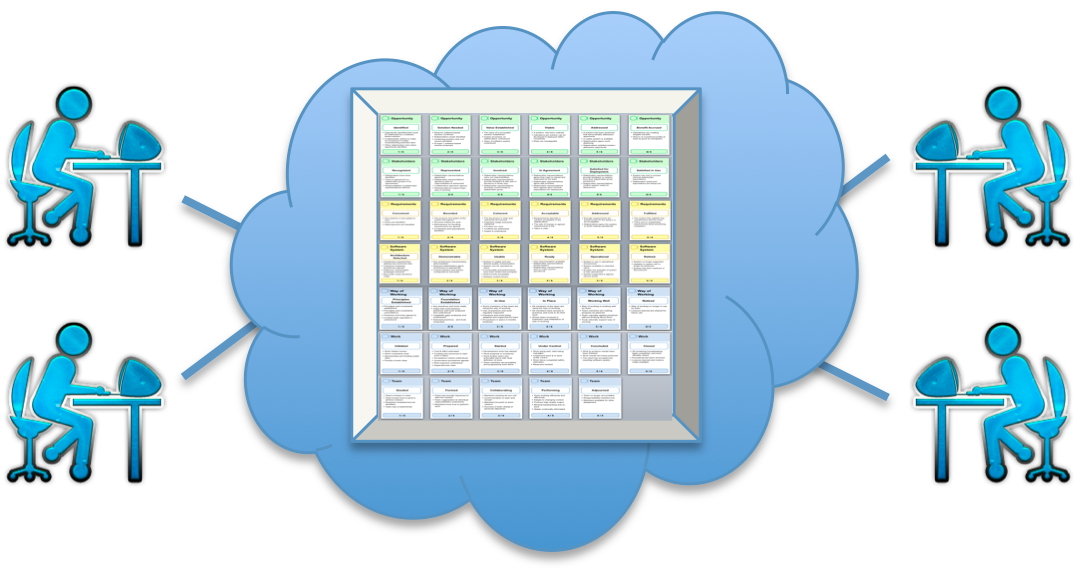
\includegraphics[width=3.40in]{project_steering_images/DigitalEssenceBoard.png}
\caption{Digital Essence board}
\label{DigitalEssenceBoard}
\end{figure}

After the initial presentation, the alphas were introduced incrementally over a number of 30 minute sessions, in order to make the experience as lightweight as possible. Each team met individually with a faculty and applied Essence on their practicum project. As an example, here is what happened with one team over a one-month period:

\underline{\textbf{Session 1}}: The two \quotes{customer} alphas, \textbf{Opportunity} and \textbf{Stakeholder}, were introduced. The main reason for introducing these two alphas first, was simply because it generally makes sense to have a discussion around the opportunity and stakeholders early in the project and before drilling down into the details of the solution and endeavor.

\underline{\textbf{Session 2}}: After updating the progress made for the previously introduced alphas, one \quotes{solution} alpha, \textbf{Requirements}, was introduced. The rationale for introducing this alpha was based on a pain point, as the team was expressing concerns around the client's expectations and hence needed to have a discussion around project scope and success criteria in relation with the \textbf{Requirements} alpha.

\underline{\textbf{Session 3}}: After updating the progress made for previously introduced alphas, two \quotes{endeavor} alphas, \textbf{Team} and \textbf{Way of Working}, were introduced based on additional pain points. Indeed the team was having some communication issues and hence needed to have a discussion around team collaboration and way of working.

\underline{\textbf{Session 4}}: After updating the progress made for previously introduced alphas, the remaining alphas were introduced for completeness: \textbf{Software System} and \textbf{Work}.

For each alpha, the team identified the current state, the target state, and any work items necessary to progress from the current to the target state. The identification of the current and target states was done through an informal discussion until the team reached an agreement.

To continue the example above, during the second session the team identified \textit{Conceived} as the current state for the \textbf{Requirements} alpha and \textit{Bounded} for the target state. Indeed all the items on the \textit{Conceived} checklist were satisfied while a few items on the Bounded checklist were not satisfied. In order to achieve \textit{Bounded}, the team first needed to define the project scope and clarify the success criteria with the client, as illustrated in Figure \ref{WorkItems}. The work items were dealt with right away or added to the team's work item list or backlog.

\begin{figure}[h]
\centering
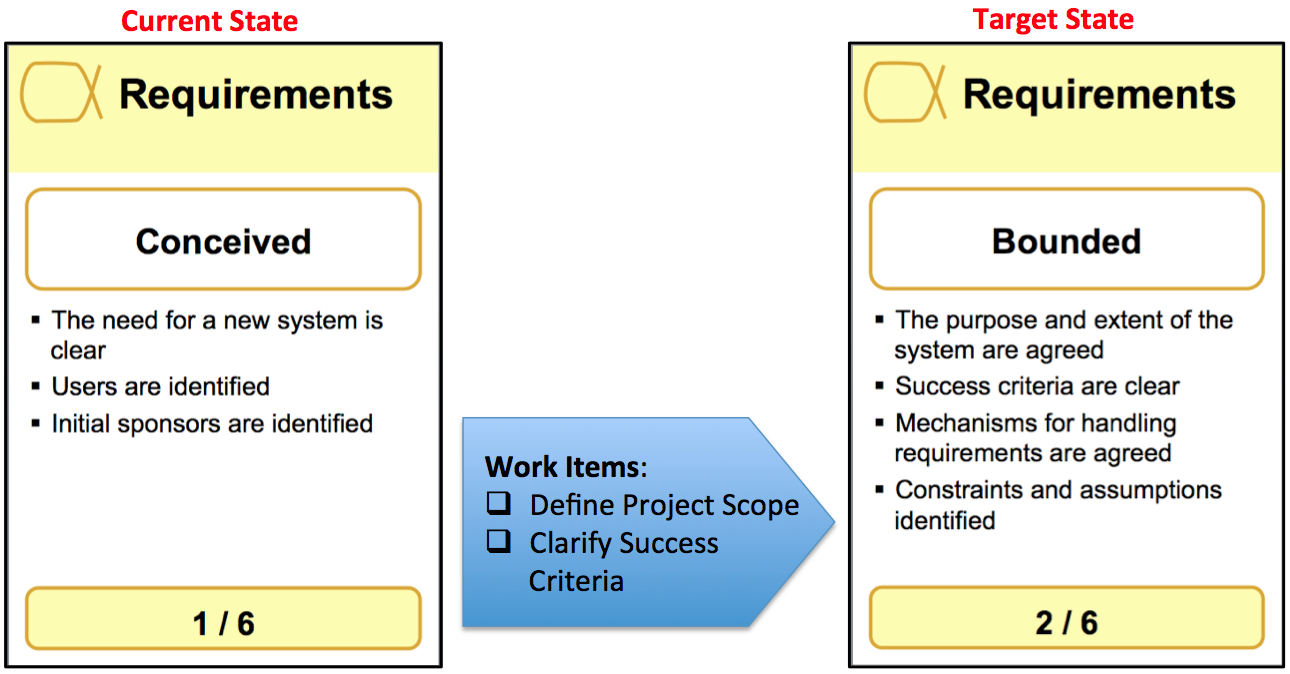
\includegraphics[width=3.30in]{project_steering_images/WorkItems.png}
\caption{Work items to reach the Bounded state}
\label{WorkItems}
\end{figure}

With mentoring from faculty, Essence was introduced to the geographically distributed teams using the incremental approach described above. For each team, and following the initial presentation of the Essence framework, four sessions of about 30 minutes long were necessary in order to introduce all the seven alphas incrementally. During each session, elements relevant to our study were jointly logged by students and faculty as described in Section \ref{UsingEssenceOnPracticumProjects} below.

\subsubsection{Second Pilot Projects - Workshop Approach}
In the Summer 2013 semester, Essence was introduced to four co-located teams at the beginning of the project. Based on our previous experience with the distributed students and armed with encouraging results (presented in Section \ref{FieldStudyAnalysis} below), we decided to speed-up the introduction process using a workshop approach. Our goal was to help the teams benefit from Essence as early as possible in the lifecycle.

The workshop was time-boxed to 90 minutes and included all students. It consisted of a general introduction of the Essence framework, the motivation for adopting the framework, together with exercises teaching each team how to apply the Essence's monitoring and steering approach on their own practicum project, one alpha at a time. Like in the first pilot projects and for the same reasons, the two green \quotes{customer} alphas, \textbf{Opportunity} and \textbf{Stakeholders}, were introduced first. Then, the remaining alphas (\textbf{Requirements}, \textbf{Software System}, \textbf{Team}, \textbf{Way of Working}, and \textbf{Work}) were introduced based on pain points when applicable, or in a random order otherwise. For each alpha, each team was tasked of identifying their project current state, target state, and any work items necessary to transition from the current to the target state. The identified work items were added to the team's work item list or backlog.

A couple of changes were introduced compared to the first pilot projects:

\begin{itemize}
    \item \textbf{Moving from physical cards to physical strips.} Handling a large set of cards could be a hassle. Therefore, we decided to create strips instead, as illustrated in Figure \ref{OneAlphaStrip}. For each alpha, one strip represents the typical sequence of states that the alpha progresses through during the project lifecycle. This way, we could easily provide the students with the information they needed to work on various alphas, one alpha at a time. Note that since the students were all physically present during the workshop, no digital boards were used.
    
    \item \textbf{Adoption of a poker game approach for state identification.} In order to remove anchoring bias, the informal way of identifying the current and target states was replaced with a \quotes{poker game} approach. In that context, each participant does a blind determination of their current state and all reveal their current state at the same time. In case of disagreement, the team discusses the different points of view until the participants reach an agreement. This technique is a simplification of Wideband Delphi \cite{StellmanAppliedPM} and agile estimation using Planning Poker \cite{GrenningPlanningPoker}, as the participants perform only one round of \quotes{estimation.} Just like Delphi and Planning Poker, the value is in the conversation, and allowing the team members to work through their different perspectives.
\end{itemize}

\begin{figure}[h]
\centering
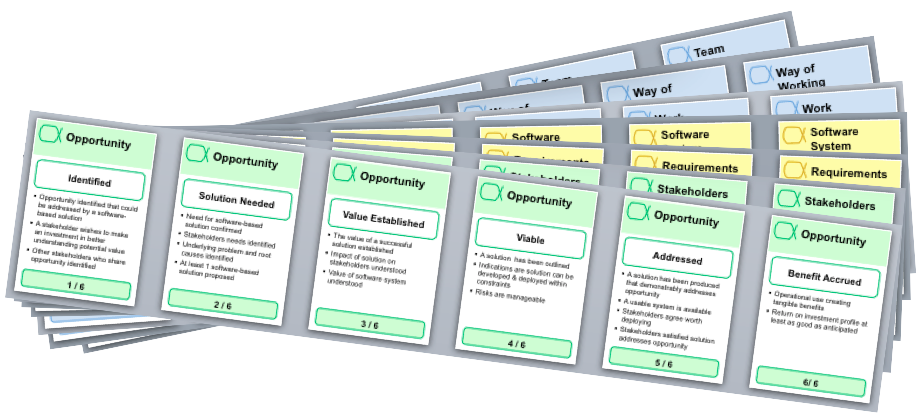
\includegraphics[width=3.30in]{project_steering_images/OneAlphaStrip.png}
\caption{One strip per alpha}
\label{OneAlphaStrip}
\end{figure}

Using the workshop approach described above, and with mentoring from faculty, Essence was introduced to the co-located teams over a 90 minutes session. On average, 10 minutes were necessary for a team to cover one alpha, and most teams were able to cover the seven alphas during the workshop. Students and faculty jointly logged elements relevant to our study as described in the following section.

\subsection{Using Essence on Practicum Projects}
\label{UsingEssenceOnPracticumProjects}
Once Essence was introduced, the teams were asked to continue leveraging the approach during the remainder of their project. Each team met on a regular basis (mostly weekly) for a 30 minutes session. During each session, the team reviewed most or all of the alphas. For each alpha, the team identified their project's current states following the poker game approach. The team would consider work items necessary to transition from the current state to the target state. Any new identified work items were added to the team's work item list or backlog. Teams were encouraged to act on their work items as soon as possible to accelerate their state progression

A faculty member was present to facilitate each session. Faculty involvement was kept at a minimum to limit influencing the steering of the project. The faculty's role was constrained to guiding the team through the application of the Essence monitoring and steering approach, and to validating the objectivity of the team's self-assessment of their project state. By listening to the team's discussions, and asking clarification questions as needed, the faculty gauged the project state. At times, this helped reduce the tendency of some teams to be overly pessimistic or optimistic about the project state.

For the purpose of the field study, progress and work items were recorded jointly by the students and faculty using the teams' Essence progress log, as shown in Table \ref{EssenceProgressLog}.

\begin{table*}[]
\centering
\caption{Essence progress log}
\renewcommand{\arraystretch}{1.4}
\label{EssenceProgressLog}
\begin{tabular}{|l|l|l|p{3.25in}|}
\hline
\multicolumn{4}{|l|}{Date:}                                         \\ \hline
\hline
Alpha           & Current State & Target State & Work Items / Notes \\
\hline
Stakeholders    &               &              &                    \\ \hline
Opportunity     &               &              &                    \\ \hline
Requirements    &               &              &                    \\ \hline
Software System &               &              &                    \\ \hline
Team            &               &              &                    \\ \hline
Way of Working  &               &              &                    \\ \hline
Work            &               &              &                    \\ \hline
\end{tabular}
\end{table*}

% \begin{figure}[h]
% \centering
% \includegraphics[width=3.30in]{project_steering_images/EssenceProgressLog.png}
% \caption{Essence progress log}
% \label{EssenceProgressLog}
% \end{figure}

The distributed students mostly used their digital Essence board, while the co-located teams used both digital Essence board and strips. Some students kept their strips handy and used them throughout the project lifecycle while others preferred to rely on the digital board.

At the end of the projects a survey was sent to the students, including the following questions:

\textbf{Survey Question 1}: What did you like the most about Essence? 

\textbf{Survey Question 2}: What did you like the least about Essence? 

\textbf{Survey Question 3}: In using Essence, did you adopt a practice that you wouldn't have? Or did you adopt it earlier than you would have without using Essence? (Please explain)

\textbf{Survey Question 4}: Was following the Essence approach worth your time? (Please explain why or why not)

\textbf{Survey Question 5}: Would you use Essence on your next project? (Please explain why or why not)

\textbf{Survey Question 6}: Anything else that we should know?

\section{FIELD STUDY ANALYSIS \& INTERPRETATION}
\label{FieldStudyAnalysis}
Our research questions relate to the value provided by the SEMAT Essence's monitoring and steering approach. The researchers measured the qualitative value based on students' feedback collected mostly during the weekly SEMAT sessions, course reflection reports, and final survey. The researchers measured the quantitative value based on alpha state progression as well as the number of work items generated during the weekly SEMAT sessions and allowing bringing the project to a higher state. Refer to Figure \ref{FieldStudyRowData} in the Appendix for the raw data collected on alpha state progression, and to Figure \ref{NewWorkItemsGenerated} under Research Question 3 for the number of work items generated by the approach per week.

\textbf{Research Question 1}: Does the SEMAT Essence's monitoring and steering approach provide value to the project team?

Our field study shows that students receive value from SEMAT Essence's monitoring and steering approach provided by the kernel alphas and their states. In our survey, 90\% of the students said that following the approach was worth their time (80\% of the students participated in the survey.) Similarly, 80\% said that they will use the approach on their next project.

By following the approach, project teams monitored their progression through the Essence states over time, as illustrated in Figure \ref{AlphaProgressionColocated4} for team Co-located-4. Every week this team generated on average 6 new work items during their SEMAT session, and then acted on these work items in order to bring the project to a higher state.

\begin{figure}[h]
\centering
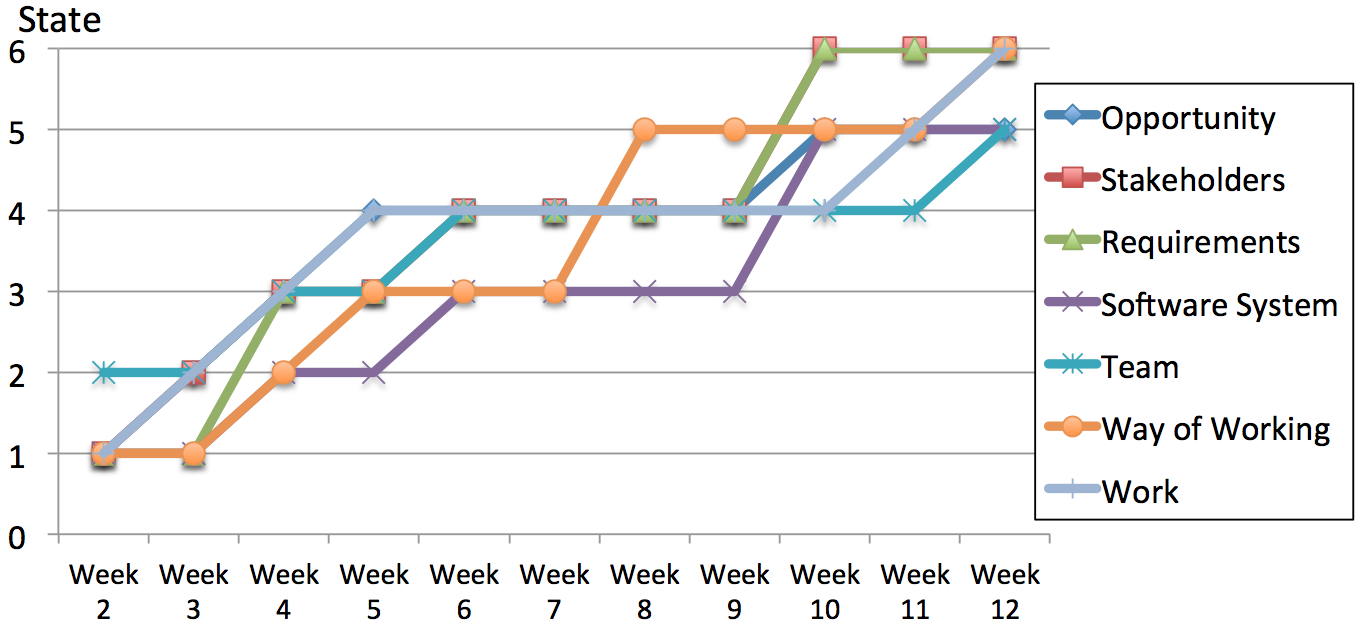
\includegraphics[width=3.30in]{project_steering_images/AlphaProgressionColocated4.png}
\caption{Alpha progression for team Co-located-4}
\label{AlphaProgressionColocated4}
\end{figure}


In conclusion, most students have a positive perception of this approach as it helps them make decisions allowing to move their project forward.

\textbf{Research Question 2}: How does SEMAT Essence's monitoring and steering approach provide value to the project team?

The benefits that a project team receives from SEMAT Essence's monitoring and steering approach come primarily from the discussions that occur when the team is covering the various alphas. The discussions enable the team to pause and assess the situation:

\begin{itemize}
    \item \textbf{The team steps back from its daily tasks and examines its project holistically.} One student noted: \participantQuote{Essence gives us a chance to step back and look at the project as a whole, from a bird's-eye view. There are aspects that we tend to ignore when focused on the technology. Essence is very useful, because it makes me think about these particular aspects.} Similarly, another student noted: \participantQuote{I like the fact that Essence provides a structured way of thinking about critical aspects of the project at different stages of the project. Without Essence, our team could have overlooked some of these aspects.} Stepping back and looking at the project holistically is a healthy exercise providing the distance and perspectives needed to understand a situation, reflect, and make decisions. When asked about what they like the most about Essence, most students mentioned reflection or retrospective. For instance one student noted: \participantQuote{Though the team was holding retrospectives every week already, having Essence discussions be a part of it allowed the team to touch on important aspects of the project.}
    
    \item \textbf{The team records progress accomplished and identifies what remains to be done.} When asked about what she liked the most about Essence, one student answered: \participantQuote{The choice of alphas: they seem to be exactly the right areas to monitor to promote the success of a software project.} The Essence mechanism for monitoring progress is illustrated in Figure \ref{ProjectStateDistributed3}. The chart shows the progress made by team Distributed-3 at week 5, compared to the practicum target state established by faculty. The team has been making good progress towards the target goal in most dimensions except \textbf{Software System} that lags at state 1 (\quotes{\textit{Architecture Selected}}). This situation served as a red flag and a reminder that the team needed to focus its effort on taking their software system to the next level. The approach was used as a similar risk management mechanism in other instances. When asked if he would use Essence on his next project, one student answered: \participantQuote{Yes, it 's great for team reflection and risk management.}
    
    \item \textbf{The team seeks guidance on what directions to take and identifies goals to transition to a higher project state.} Team Distributed-1 noted: \participantQuote{Essence gives us structure and direction.} Another student commented: \participantQuote{Essence is useful, as it gives you an agenda or checklist based on various dimensions (even though I was skeptical at first).} Essence provides a simple project steering mechanism. For each alpha, the identified target state provides the direction to take, and its checklist provides goals to reach. For instance and to continue the example above, during week 5 team Distributed-3 identified \quotes{\textit{Demonstrated}} as its target state for \textbf{Software System}, with a number of goals including demonstrating the key architecture characteristics, as illustrated in Figure \ref{ProjectStateDistributed3}.
    
    \item \textbf{The team decides what to do to reach the target goals. Once the team identifies the goals, the team members rely on their software engineering knowledge and experience to decide how to reach these goals.} Indeed, Essence does not prescribe the use of any existing method (like Scrum or XP) or set of practices or work items. Instead, the team has the flexibility to leverage any method or set of practices that best suit their needs, and decide what work items to perform to reach the goals set by the target state. As a consequence, our seven practicum teams were able to leverage Essence even though they all used a different set of software engineering practices. When asked if he would use Essence on his next project, one student answered: \participantQuote{Yes, especially with a project team that is not used to the same software engineering process. In that instance Essence is a backdrop at the basis of the communication about all the considerations for the success of the project.} Another student added: \participantQuote{It is simple, lightweight and useful.}
\end{itemize}

\begin{figure}[t]
\centering
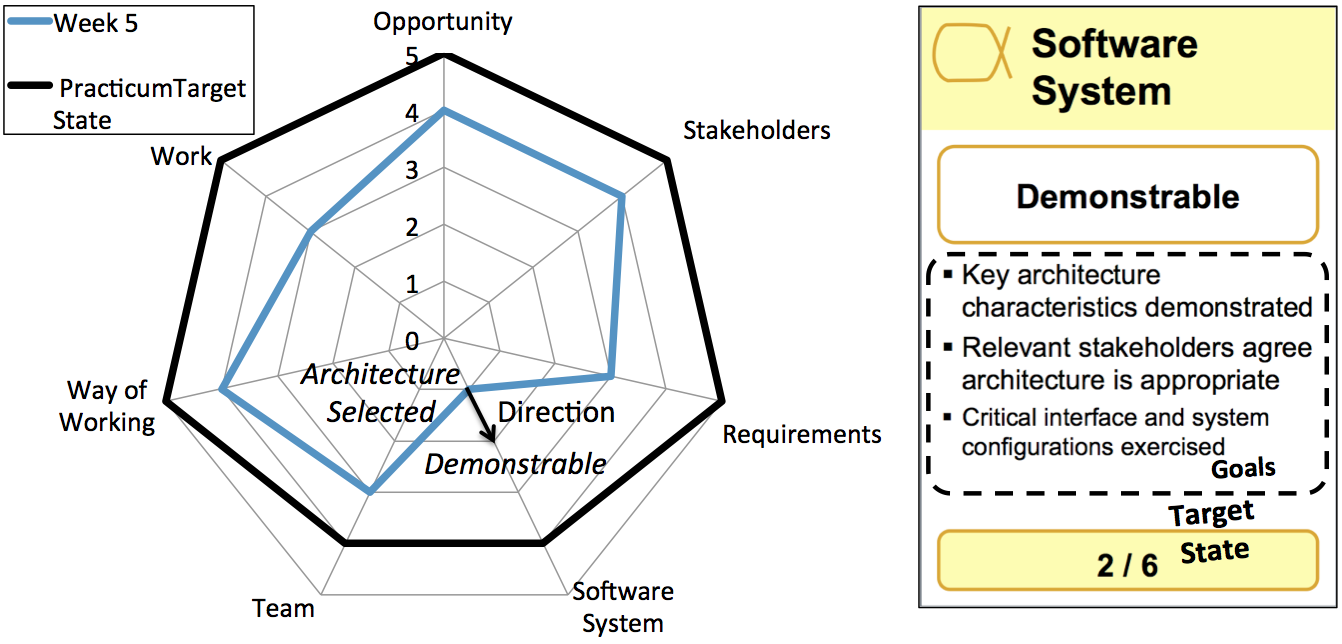
\includegraphics[width=3.30in]{project_steering_images/ProjectStateDistributed3.png}
\caption{Project state for team Distributed-3 at week 5, with direction and goals for Software System}
\label{ProjectStateDistributed3}
\end{figure}


The team accelerates its state progression by acting on its work items as soon as possible and iterating through the steps described above. Figure \ref{EssenceMonitoringLoop} illustrates this iterative process.

\begin{figure}[t]
\centering
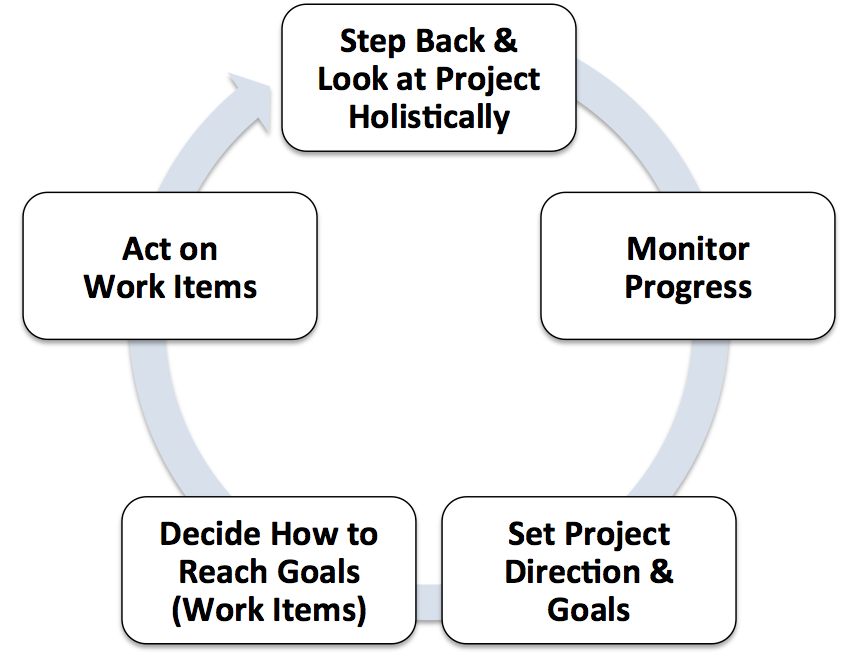
\includegraphics[width=3.30in]{project_steering_images/EssenceMonitoringLoop.png}
\caption{Essence monitoring and steering loop}
\label{EssenceMonitoringLoop}
\end{figure}

In answer to our second research question, the approach adds value by providing the project team with a holistic view of the project, a mechanism for monitoring progress and steering projects, as well as an effective structure for team reflection and risk management. This is provided in a simple, lightweight, non-prescriptive and method-agnostic fashion.

\textbf{Research Question 3}: When in the project lifecycle does the SEMAT Essence's monitoring and steering approach add value?
The value that the teams receive from SEMAT Essence's monitoring and steering approach varies over the project lifecycle. Our study shows that most value is generated at the beginning of the project and that it decreases thereafter. Here are some illustrating quotes:
\begin{itemize}
    \item When asked if following the Essence approach was worth their time, 20\% of the students who answered yes to the question qualified their answers as follows: \participantQuote{Yes, it helped us at the beginning of the project}, or \participantQuote{Yes, it was worth my time in the first half of the project.}
    
    \item Among the students who mentioned that they would use Essence on their next project, one qualified her answer as follows: \participantQuote{Yes, but only at the beginning of the project.}
    
    \item When asked what he liked the least about Essence, one student answered: \participantQuote{Essence lost value once the project settled because we dead ended on a set of cards.} Another student added: \participantQuote{Essence is useful in the planning stages. Later on its usefulness is dying down. If you spend multiple weeks on one card, then spending time looking at it is less helpful.} This opinion is shared by about 50\% of the students.
    
    \item The faculty in charge of the practicum course, and who has taught the course for 10 years, noted: \participantQuote{Compared to previous years, I see a much better early project organization with lot less floundering. I hope that we keep using Essence in the future. We should definitely keep it at the beginning of the projects.}
\end{itemize}

The alpha progression of team Co-located-3 illustrates the decrease in value, as seen in Figure \ref{AlphaProgressionColocated3}. The chart shows that the team progresses well during the first half of the project, then reaches a plateau or stable state during a few weeks, before progressing again at the end of the project. This picture represents most teams' progressions.

\begin{figure}[t]
\centering
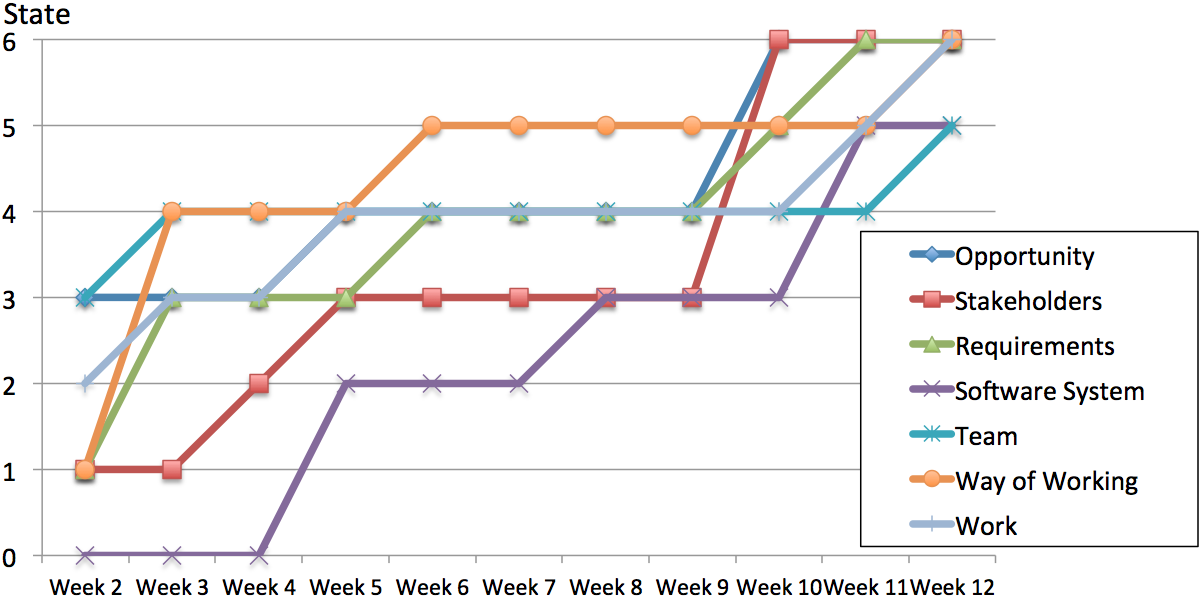
\includegraphics[width=3.30in]{project_steering_images/AlphaProgressionColocated3.png}
\caption{Alpha progression for team Co-located-3}
\label{AlphaProgressionColocated3}
\end{figure}


By analyzing the work items generated by the team during the weekly SEMAT sessions, we find that the initial progression in Figure \ref{AlphaProgressionColocated3} is driven by those work items. Indeed these work items significantly contribute to bringing the project to a higher state. However, the final progression is done independently of Essence as the approach generates few work items at the end of the project. Most teams experienced this phenomenon, as illustrated in Figure \ref{NewWorkItemsGenerated} showing a consistent drop of work items over time.

\begin{figure}[t]
\centering
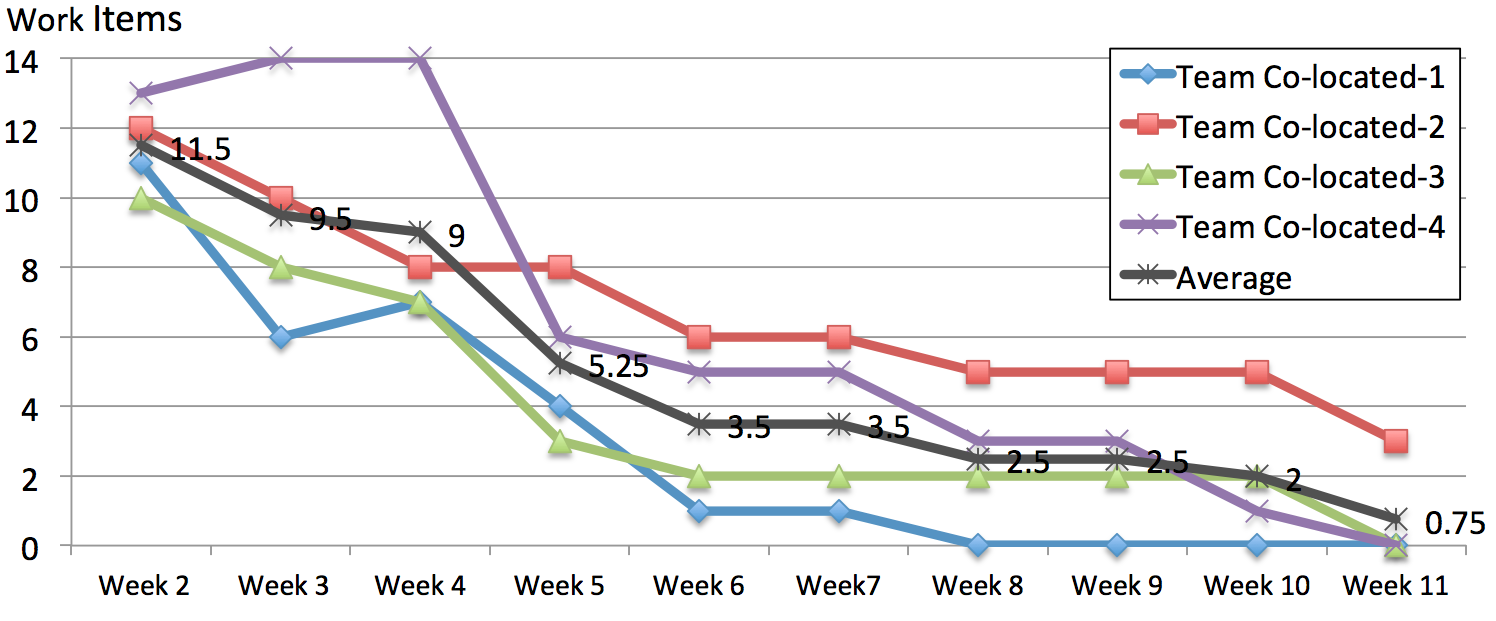
\includegraphics[width=3.30in]{project_steering_images/NewWorkItemsGenerated.png}
\caption{New work items generated per week}
\label{NewWorkItemsGenerated}
\end{figure}

Despite the value decrease, the students' perception of the approach remains positive by the end of the project according to the survey responses. Indeed a majority of students answered without qualification that they found Essence worth their time and will use the approach on their next project. A majority of students also mentioned reflection or retrospective as a strength of the approach. One student mentioned: \participantQuote{Even though we are not generating new tasks, the [SEMAT] meetings remain useful as they give us the opportunity to reflect upon our project.} Similarly, team Distributed-1 noted in its reflection report: \participantQuote{The team was pleased to see that Essence covered `The Way of Working' as well as ‘The Team'. These two topics generated useful team introspection at the beginning of the practicum and were nice reminders that the team does constant checkups for the overall condition of the members and the project.}

In conclusion, the SEMAT Essence's monitoring and steering approach provided by the kernel alphas and their states is most effective at the beginning of the project. The effectiveness decreases over time. Indeed, the approach gradually loses its ability to enable the team to steer the project by generating new work items leading to a higher project state. The reasons behind the value decrease are explored in the next research question. However, most teams continue to perceive value throughout the lifecycle out of the approach reflection mechanism.

\textbf{Research Question 4}: What are the limitations to the approach's effectiveness?

The previous section shows that the effectiveness of the approach decreases over time. This phenomenon could be explained by a number of factors. One factor relates to the fact that the need for the approach varies throughout the project lifecycle. For instance, as the project team matures and becomes a high-performing team producing high quality outcome, it becomes a self-steering team requiring less support from the approach. Similarly, once most project risks have been mitigated, the team requires less risk management support. Therefore, unless there is a disruptive event reverting the project to a lower state, the value decrease is to be expected.

In addition, some kernel characteristics influence the value decrease. Most Essence alphas have more states supporting the progression through the initial project phase compared to later phases. Figure \ref{NumberOfAlphaStatesPerRUPPhase} illustrates this phenomenon using the RUP \cite{KrollRUP} phases (Inception, Elaboration, Construction, and Transition) as an example. The chart shows that for most alphas, the number of states per phase is higher in Inception compared to the other phases. For five out of seven alphas, there is only one state in Construction. Most project teams spend the majority of their time in Construction. As a result, for these alphas the teams end-up remaining in the same state during their entire Construction phase. This lack of alpha states covering the Construction phase might be due to the fact that most of the technical work done in Construction is practice-specific, and therefore not supported by the universal kernel. Further investigations are necessary to identify potential ways to extend the kernel so it better supports the work done during Construction.

\begin{figure}[t]
\centering
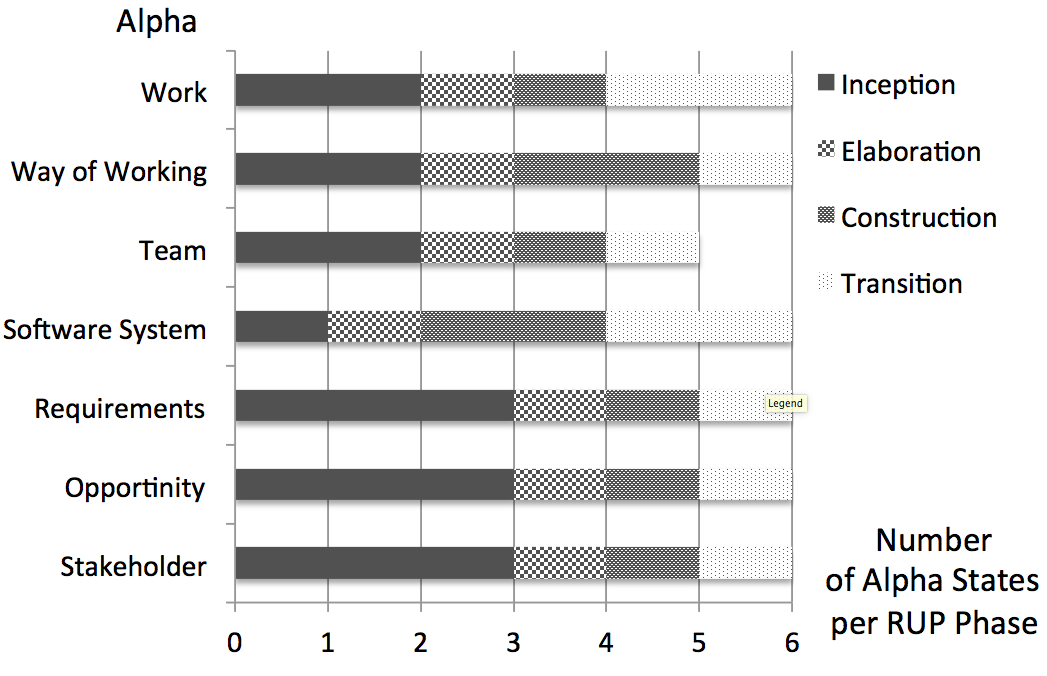
\includegraphics[width=3.30in]{project_steering_images/NumberOfAlphaStatesPerRUPPhase.png}
\caption{Number of alpha states per RUP phase}
\label{NumberOfAlphaStatesPerRUPPhase}
\end{figure}

By definition, the Essence kernel is geared towards steering a project or release throughout its entire lifecycle in a fairly linear fashion dictated by the alpha state progression. By repeating through the Essence monitoring and steering loop (see Figure \ref{EssenceMonitoringLoop}), the team steers the project or release through the sequence of states for each alpha. This process is designed to support the work done at the release level and not to support the work done at the iteration level because of the following reasons:

\begin{itemize}
    \item The kernel is lifecycle-independent and therefore does not provide specific support for iterative development.
    
    \item The kernel alpha states and their checklist items are specified at the project or release level, not at the iteration level.
\end{itemize}

Consequently, we were unable to effectively leverage the approach to help steer projects during Construction on iterative projects. The teams received some guidance on iterative development from whatever method they adopted, like Scrum and XP that are optimized for iterative development.

In conclusion, the observed value decrease could be explained by three factors. The first factor is a decrease in the need for the approach as the team matures and becomes self-steering. The second factor is a front-end focus of the alphas, making the approach most effective during project initiation. The third factor relates to the definition of the kernel alpha checklists, which are specified at the project or release level, not at the iteration level. This explains the value decrease during construction on iterative projects.

As a result, the monitoring and steering mechanisms are most effective during project initiation and for monitoring and steering the work done at the project or release level. This type of work could be qualified as \quotes{universal} as it is generally common across projects. This confirms that the kernel provides effective support for universal work. Support for non-universal technical work has to come from additional practices added on top of the kernel, or by extending or altering the kernel definition.

Finally, a limitation pointed out by about 40\% of the students in the survey, is related to some ambiguity in the alpha checklists definition. For instance, one student mentioned: \participantQuote{The checklist within an alpha can have cryptic language. Sometime, the points are ambiguous.} Here are some examples of typical student reactions:

\textbf{Checklist Item}: Enough of the requirements are addressed \ldots 

\textbf{Student}: \participantQuote{What do they mean by `enough'?}

\textbf{Checklist Item}: Constraints are identified and considered. 

\textbf{Student}: \participantQuote{What kind of constraints are they talking about?}

\textbf{Checklist item}: Critical interfaces have been demonstrated. 

\textbf{Student}: \participantQuote{What do they mean by `demonstrated'?}

\textbf{Checklist Item}: The key practices and tools that form the foundation of the way-of-working are selected.

\textbf{Student}: \participantQuote{Which tools form the foundation of the way-of-working?}

Thus, a limitation to the approach effectiveness comes from some ambiguities in the alpha checklist definitions, leading to situations where the team discusses the meaning of a checklist item instead of having a conversation about the project. At times, this disrupts the flow of otherwise valuable team discussions.

\section{FROM THE EDUCATOR'S PERSPECTIVE}
This section shares some of our findings related to introducing Essence to a project team having no prior experience with the approach, together with a few words of caution related to the use or misuse of Essence for evaluation purposes.

\subsection{Incremental versus Workshop Introduction Approaches}

Our experience with both the incremental and workshop approaches to introducing Essence indicates that both have value and that adoption resistance drives which approach is best for the situation.

\subsubsection{Incremental}
The incremental introduction approach brings immediate value to the teams, as noted by team Distributed-2 in its reflection report: \participantQuote{The team found Essence valuable right from the start. [...] it helped manage the direction and organization of the team by examining overlooked aspects of the project.} For instance, during the first session, this team identified the work items \quotes{Understand the risks and constraints} and \quotes{Identify all stakeholders} based on its discussion around the \textbf{Opportunity} alpha and \textbf{Stakeholder} alpha respectively. Some previous practicum teams overlooked these kinds of discussions and work items. However, this approach delays many important conversations until all the alphas are introduced.

This approach has minimum perceived overhead. In our case, introducing Essence incrementally required only a weekly session of 30 minutes, during a five weeks period.

When adoption resistance might be an issue, we recommend introducing the approach incrementally through a series of regular (e.g. weekly) and short (e.g. 30 minutes) sessions. We also recommend having one dedicated faculty or coach per team.

\subsubsection{Workshop}
The workshop introduction approach introduces all the alphas at once, hence enabling the team to look at its project holistically while having conversations covering the various project's dimensions as early as possible.

This approach requires that each team invest in one upfront workshop during which the team starts applying Essence directly to its current project. During our 90 minutes introduction workshop, 10 minutes were needed to set the context and motivate the exercise. The remaining 80 minutes was enough time for most teams to have a substantial conversation about their perception of the project's current state and to generate work items to make forward progress. On average, 10 minutes were necessary for a team to cover one alpha, and most teams were able to cover the seven alphas during the workshop. However, our largest team of five members took an average of 20 minutes per alpha and hence had to complete the exercise during a follow-up session. The size of the team as well as internal disagreements generated some longer conversations.

We recommend adjusting the workshop duration based on the team size and any other known parameters that might influence the length of the conversations, like team dynamic or project uncertainty. We also recommend having one dedicated faculty or coach per team.

Table \ref{ComparingWorkshopAppoaches} summarizes and compares the incremental and workshop introduction approaches. We recommend the workshop approach when introducing Essence, unless faced with initial adoption resistance that may require a slower incremental approach.

\begin{table}[]
\centering
\renewcommand{\arraystretch}{1.4}
\caption{Comparison of introduction approaches}
\label{ComparingWorkshopAppoaches}
\begin{tabular}{|p{0.6in}|p{1.1in}|p{1.1in}|}
\hline
Approach      & Incremental                                                                 & Workshop  \\
\hline
Description   & Essence alphas are introduced incrementally over a number of short sessions & Essence alphas are introduced all at once during a single session \\
\hline
Benefits      & Brings immediate value with minimum overhead                                & Brings immediate and optimum value (all alphas are covered)       \\
\hline
Drawbacks     & Full benefit is delayed until complete introduction of alphas               & Requires initial overhead                                         \\
\hline
When to Apply & In case of adoption resistance                                              & Always, except in case of adoption resistance  \\                  
\hline
\end{tabular}
\end{table}

Given our recommendation of one faculty per team, in the future, we plan on introducing Essence and conducting a full assessment during a 90-minute team meeting. In a course with five teams, scheduling five separate team meetings is easier than trying to do five simultaneous team meetings with five instructors.

Following the introduction of Essence, we recommend that each project team continue to meet on a regular (e.g. weekly) basis for a short (e.g. 30 minutes) session throughout the initial project phase. Once a team reaches \quotes{construction} and becomes a high-performing team producing high quality outcome, the frequency of the sessions could decrease because the team needs less support from the approach.

\subsection{Alpha Introduction Order}
Participants can be overwhelmed when shown all the states for all the alphas at once. Introducing the alphas one at a time solves this problem, whether this is done incrementally over a series of meetings or during a single session or workshop.

We recommend introducing the \textbf{Stakeholder} and \textbf{Opportunity} alphas (aka the customer dimension) first, since it generally makes sense to have a discussion around this dimension before drilling down into the details of the solution and endeavor. We introduce \textbf{Stakeholder} prior to \textbf{Opportunity} since many participants find it easier to relate to the \textbf{Stakeholder} alpha than the abstract \textbf{Opportunity} alpha. The other alphas could be introduced as needed based on pain points. When in doubt about which alpha to introduce next, one alpha could be selected randomly. Indeed, the value is in having a holistic view of the project, therefore looking at any dimension has potential benefits.

\subsection{A Word of Caution}
As noted by William Cameron \cite{CameronSociologicalThinking}, \quotes{not everything that can be counted counts, and not everything that counts can be counted.} This is especially true when it comes to individual and team performance evaluation, where using metrics could be dangerous. Inappropriate metrics could be used (like measuring a developer performance based on the number of lines of code produced), metrics could be gamed, and metrics do not give the full picture.

As an example, Figure \ref{AvoidThisKindOfComparison} shows the final state of our distributed teams at the end of their project. From the chart, one might infer that Team Distributed-3 outperformed Team Distributed-1, which in turn outperformed Team Distributed-2 that lagged behind. In fact, despite having the highest project state, Team Distributed-3's work was slightly disappointing according to both the clients and faculty. The team ended-up with a lower grade compared to the other teams. This was due to quality issues during various product demonstrations and a lack of architecture documentation that surfaced during the team final presentation. This makes the team self-assessment of the \textbf{Software System} alpha and therefore of its overall project state questionable. Team Distributed-2 lagged only behind because the initial solution proposed by the client turned out to be infeasible, and the team did an excellent job redirecting the project into a constructive direction and hence earned an excellent grade. The routinely low \textbf{Software System} alpha state served as a red flag for risk management purposes, not evaluation purposes.

\begin{figure}[t]
\centering
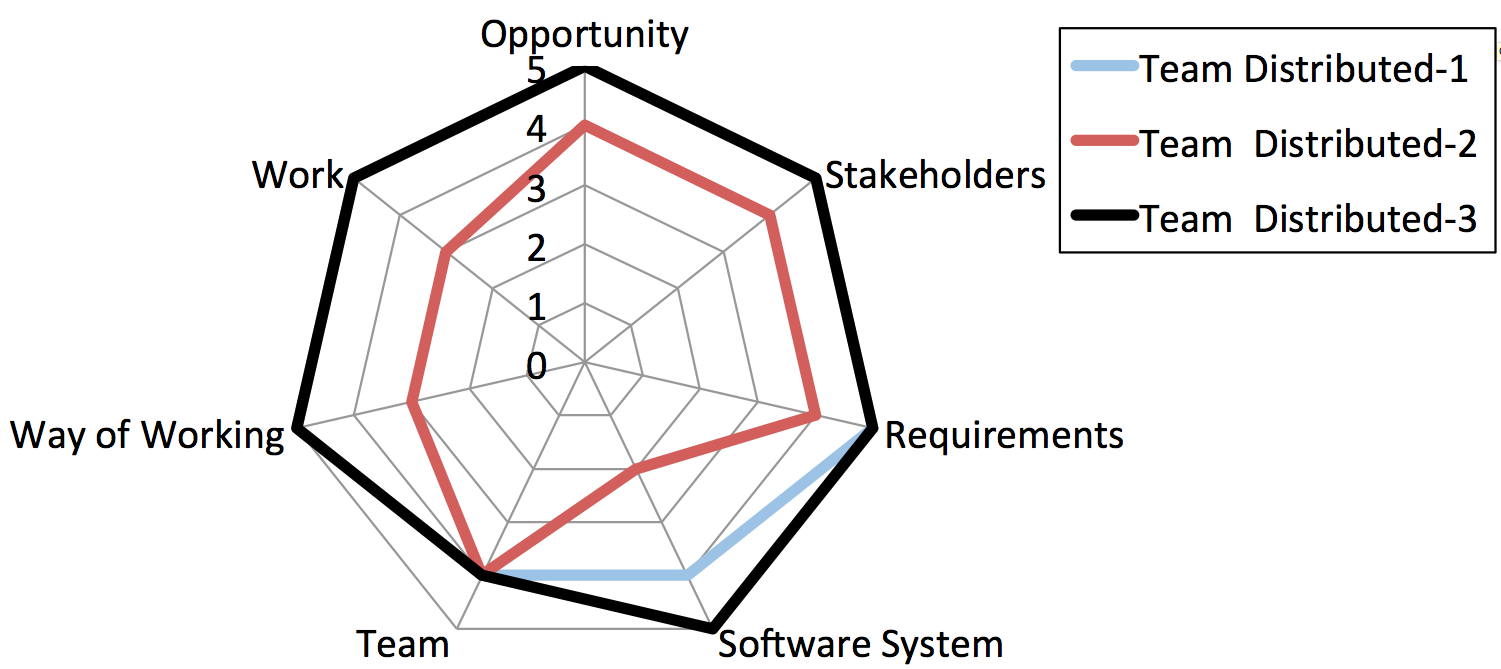
\includegraphics[width=3.30in]{project_steering_images/AvoidThisKindOfComparison.png}
\caption{Final project state of the distributed teams: Avoid this kind of comparison}
\label{AvoidThisKindOfComparison}
\end{figure}


In conclusion, we recommend leveraging the approach to identify projects at risk rather than for performance evaluation purposes. Some teams might be only ahead because they are overly optimistic about their project state, while others might be behind because of circumstances beyond their control.

\section{CONCLUSION}
This paper presents the results of a field study aiming at understanding the value project teams receive from following the SEMAT Essence's monitoring and steering approach provided by the Essence kernel alphas and their states. The study involved seven teams of master students with no prior knowledge of Essence.

The study validated our research hypothesis by showing that the approach provides student teams with a simple, lightweight, non-prescriptive and method-agnostic way to examine their projects holistically, structure team reflections, manage risks, monitor progress and steer their projects. Compared to the ten previous years, the faculty in charge of the practicum course noted that there was \participantQuote{much better early project organization with a lot less floundering.} Indeed, the approach enables students to learn to steer projects effectively by addressing the various dimensions of software engineering.

The study also highlighted that the monitoring and steering mechanisms are most effective during project initiation and for monitoring and steering the work done at the project or release level. This type of work could be qualified as \quotes{universal} as it is generally common across projects. This confirms that the kernel provides an effective support for universal work. Support for non-universal technical work should come from additional practices added on top of the kernel, or by extending or altering the kernel definition.

The results of this paper are limited to evaluating the effectiveness of the Essence approach when a facilitator is involved. Even though faculty involvement was kept at a minimum to limit influencing the students, a faculty served as facilitator during the SEMAT meetings throughout the practicum projects. More research is necessary to assess the effectiveness of the approach without facilitators.

The project context was fairly similar for all teams, except for their geographic distribution and average work experience. While the study has not revealed any influences of these contextual factors on the approach's effectiveness, additional data is required to confirm or refute any impact. The Essence steering and monitoring approach appears equally applicable to both co-located and geographically distributed teams.

We are currently working with another set of practicum teams at Carnegie Mellon University in Silicon Valley to gather more data necessary to evaluate the SEMAT Essence's monitoring and steering approach, with a focus on both effectiveness of the approach and accuracy of the model.

\section{ACKNOWLEDGMENTS}
We would like to acknowledge the contributions of all the reviewers, and thank them for their insightful comments on early drafts of this paper. A special thanks to Hakan Erdogmus and Maria Nelson for their thorough reviews and invaluable suggestions, and to Ed Katz for recommending that we conduct our field study in the context of his practicum course and for his support throughout the study. Finally, we would like to warmly thank the students who participated in the study, for their openness and insights.

\section{APPENDIX}
Figure \ref{FieldStudyRowData} below provides the reader with the field study row data on alpha state progression. Each number in bold (from 1 to 6) represents an alpha state. Each number in italic (from 2 to 15) represents the week during which the team reaches the state. For instance, team Distributed-1 reaches the \textbf{Stakeholder} state 1 at week 2. Two or more italic numbers in one cell reflects a state backtracking. For instance, team Co-located 2 reaches the \textbf{Team} state 3 at week 2. The team then progresses to a higher state, but backtracks to state 3 at week 10.

\begin{figure*}[h]
\centering
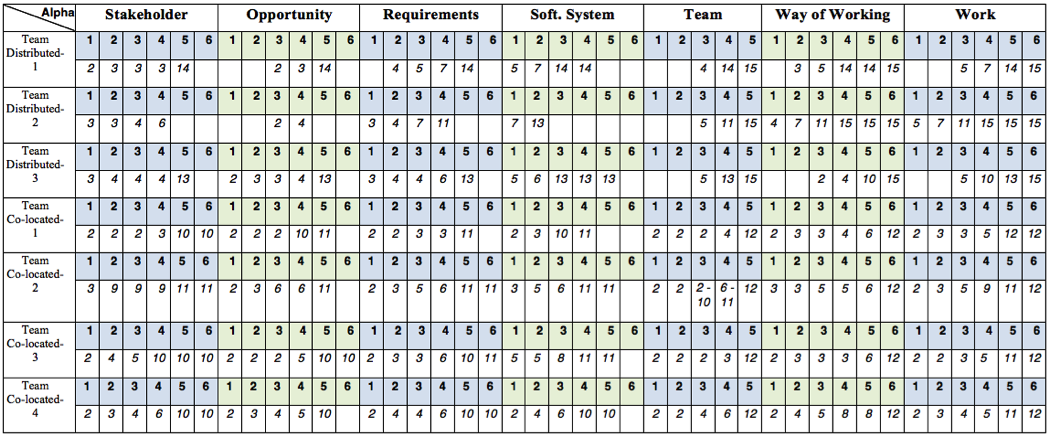
\includegraphics[width=6.80in]{project_steering_images/FieldStudyRowData.png}
\caption{Field study row data on alpha state progression}
\label{FieldStudyRowData}
\end{figure*}


% \begin{table*}[]
% \centering
% \renewcommand{\arraystretch}{1.3}
% \caption{Field study row data on alpha state progression}
% \label{FieldStudyRowDatal}
% \begin{tabular}{|l|l|l|l|l|l|l|l|l|l|l|l|l|l|l|l|l|l|l|}
% \hline
%                   & \multicolumn{6}{l|}{Stakeholders} & \multicolumn{6}{l|}{Opportunity} & \multicolumn{6}{l|}{Requirements} \\ \hline
%                   & 1   & 2   & 3   & 4   & 5   & 6   & 1   & 2   & 3  & 4   & 5   & 6   & 1   & 2   & 3   & 4   & 5   & 6   \\ \hline
% Team Distributed-1 & 2   & 3   & 3   & 3   & 14  &     &     &     & 2  & 3   & 14  &     &     & 4   & 5   & 7   & 14  &     \\ \hline
% Team Distributed-2 & 3   & 3   & 4   & 6   &     &     &     &     & 2  & 4   &     &     & 3   & 4   & 7   & 11  &     &     \\ \hline
% Team Distributed-3 & 3   & 4   & 4   & 4   & 13  &     & 2   & 3   & 3  & 4   & 13  &     & 3   & 4   & 4   & 6   & 13  &     \\ \hline
% Team Co-located-1  & 2   & 2   & 2   & 3   & 10  & 10  & 2   & 2   & 2  & 10  & 11  &     & 2   & 2   & 3   & 3   & 11  &     \\ \hline
% Team Co-located-2  & 3   & 9   & 9   & 9   & 10  & 11  & 2   & 3   & 6  & 6   & 11  &     & 2   & 3   & 5   & 6   & 11  & 11  \\ \hline
% Team Co-located-3  & 2   & 4   & 5   & 10  & 10  & 10  & 2   & 2   & 2  & 5   & 10  & 10  & 2   & 3   & 3   & 6   & 10  & 11  \\ \hline
% Team Co-located-4  & 2   & 3   & 4   & 6   & 10  & 10  & 2   & 3   & 4  & 5   & 10  &     & 2   & 4   & 4   & 6   & 10  & 10  \\ \hline
% \end{tabular}
% \end{table*}


% \begin{table*}[]
% \centering
% \caption{My caption}
% \label{my-label}
% \begin{tabular}{|l|l|l|l|l|l|l|l|l|l|l|l|l|l|l|l|l|l|l|l|l|l|l|l|l|l|l|l|l|l|l|l|l|l|l|l|l|l|l|l|l|l|}
% \hline
%                   & \multicolumn{6}{l|}{Stakeholders} & \multicolumn{6}{l|}{Opportunity} & \multicolumn{6}{l|}{Requirements} & \multicolumn{6}{l|}{Software System} & \multicolumn{5}{l|}{Team} & \multicolumn{6}{l|}{Way of Working} & \multicolumn{6}{l|}{Work} \\ \hline
%                   & 1   & 2   & 3   & 4   & 5   & 6   & 1   & 2   & 3  & 4   & 5   & 6   & 1   & 2   & 3   & 4   & 5   & 6   & 1    & 2   & 3    & 4    & 5   & 6   & 1   & 2  & 3  & 4   & 5   & 1   & 2   & 3   & 4    & 5    & 6   & 1  & 2  & 3 & 4 & 5  & 6  \\ \hline
% Team Distributed-1 & 2   & 3   & 3   & 3   & 14  &     &     &     & 2  & 3   & 14  &     &     & 4   & 5   & 7   & 14  &     & 5    & 7   & 14   & 14   &     &     &     &    & 4  & 14  & 15  &     & 3   & 5   & 14   & 14   & 15  &    &    & 5 & 7 & 14 & 15 \\ \hline
% Team Distributed-2 & 3   & 3   & 4   & 6   &     &     &     &     & 2  & 4   &     &     & 3   & 4   & 7   & 11  &     &     &      &     &      &      &     &     &     &    &    &     &     &     &     &     &      &      &     &    &    &   &   &    &    \\ \hline
% Team Distributed-3 & 3   & 4   & 4   & 4   & 13  &     & 2   & 3   & 3  & 4   & 13  &     & 3   & 4   & 4   & 6   & 13  &     &      &     &      &      &     &     &     &    &    &     &     &     &     &     &      &      &     &    &    &   &   &    &    \\ \hline
% Team Co-located-1  & 2   & 2   & 2   & 3   & 10  & 10  & 2   & 2   & 2  & 10  & 11  &     & 2   & 2   & 3   & 3   & 11  &     &      &     &      &      &     &     &     &    &    &     &     &     &     &     &      &      &     &    &    &   &   &    &    \\ \hline
% Team Co-located-2  & 3   & 9   & 9   & 9   & 10  & 11  & 2   & 3   & 6  & 6   & 11  &     & 2   & 3   & 5   & 6   & 11  & 11  &      &     &      &      &     &     &     &    &    &     &     &     &     &     &      &      &     &    &    &   &   &    &    \\ \hline
% Team Co-located-3  & 2   & 4   & 5   & 10  & 10  & 10  & 2   & 2   & 2  & 5   & 10  & 10  & 2   & 3   & 3   & 6   & 10  & 11  &      &     &      &      &     &     &     &    &    &     &     &     &     &     &      &      &     &    &    &   &   &    &    \\ \hline
% Team Co-located-4  & 2   & 3   & 4   & 6   & 10  & 10  & 2   & 3   & 4  & 5   & 10  &     & 2   & 4   & 4   & 6   & 10  & 10  &      &     &      &      &     &     &     &    &    &     &     &     &     &     &      &      &     &    &    &   &   &    &    \\ \hline
% \end{tabular}
% \end{table*}

% \chapter{Essence Green Lighting}
\section{Abstract}

Many software engineering curriculum conclude with a
practicum or capstone project course. For courses involving external
clients, the course owner typically follows a Request for Proposal
process to vet (or green-light) qualified clients and projects.

Even though green-lighting projects does not guarantee project success, 
the goal is to reduce risks by systematically examining each proposal to identify
potential problems that the instructor could solve, mitigate against, 
or simply decide not to deal with by rejecting the proposal.

We propose and evaluate a Green-Lighting Approach based on the
SEMAT (Software Engineering Method and Theory) Essence framework. 
Our objective is to identify if such a framework could improve the Request for Proposal process 
at Carnegie Mellon University in Silicon Valley and other universities.

We conducted a case study by observing and interviewing the
course owner, examining a group of proposals, and identifying issues
with the current proposal process and practicum projects.
We proposed a green-lighting project state that, based upon Essence Alphas,
describes the minimal and ideal states that a project proposal should achieve to be accepted. 

The Green-Lighting Approach generated conversations among the faculty 
that clarified the guidelines for accepting and prioritizing proposals and identified deficiencies in our Request for Proposal. Additional work is required to refine the proposed Green-Lighting Approach based on current findings and further validate the approach.
  
Using Essence for green-lighting practicum projects in academia presents some limitations. 
The framework does not explicitly factor in business forces that affect proposal selection,
might be overly complex for the task, and might require modification with partial Alpha states. 
However, Essence provides a systematic approach for evaluating proposals based on various project dimensions. 
This approach could be used as an inspiration for deriving simpler custom green-lighting checklists. 

\section{Introduction}
\label{Introduction}

Many software engineering (SE) curricula finish with a practicum course
or capstone project \cite{GSWE}. At Carnegie Mellon
University in Silicon Valley, the curriculum culminates with a practicum
course in order for the students to demonstrate mastery of the
curriculum and to learn client management skills
\cite{Katz}. The practicum allows students to reinforce
their learning of core software engineering knowledge by applying this
knowledge to a different problem or domain. The practicum serves as
confirmation that the student has mastered the material. Earlier in the
curriculum, faculty manage the students project courses by playing the
customer or management role. The practicum provides an opportunity for
the students to work with a real client and practice client management
skills. Students actively manage the client engagement while faculty
observe and coach students without interfering unless necessary. The
students perform as a consulting team delivering a product that addresses the client's opportunity.

The university wants to increase its impact through the practicum
projects. The practicum course owner needs to find projects that
balance these goals:

\begin{itemize}
\itemsep1pt\parskip0pt\parsep0pt
\item
  maximize the students' learning experience, 
\item
  achieve a business goal or positively impact society, and
\item
  increase collaborations between university and industry. 
\end{itemize}

In order to accomplish the practicum goals, the faculty want to offer
a portfolio of projects including

\begin{itemize}
\itemsep1pt\parskip0pt\parsep0pt
\item
  a mix of project domains,
\item
  a mix of startups and established companies, and 
\item
  a mix of exploratory research and well defined
  endeavors.
\end{itemize}

Since we have a limited number of students and thus student teams, the
course owner needs to be selective about proposals with respect to these
goals. The course owner needs a systematic, non biased technique to
filter proposals.

\section{Related Work}
\label{Related Work}
Many software engineering professors have described their approach to providing a practical hands on experience. Most of the literature describes in detail how to run a team-based project course yet there is little discussion about the client selection process. 

In 1991, Shaw and Tomayko \cite{shaw1991models} examined hundreds of undergraduate software engineering courses and interviewed scores of instructors. In their technical report, they identify two major decisions that the instructor must make: 1) deciding the mixture of lecture and project components and 2) deciding the balance technical and managerial skills taught in the course. 

They describe several course models used in academia including the ``small group project'' model, ``large project team,'' model, and  ``the project only'' model. The ``small group project'' and  ``large project team'' models infuse lectures with a course long project. The ``project only'' model is typically a capstone course that focuses on the project experience.

Shaw and Tomayko discusses the importance of finding an interesting project that will motivate the students for the duration of the course, but provides no model for client selection.

In 2001, Cal Poly \cite {Turner2001} introduced a year long capstone project course. For the first two years, they relied on one industrial partner for the entire course, but due to coordination difficulties replaced the external project with a university project. No guidance is provided for project selection.

In 2002, Chamillard and Braun \cite{Chamillard2002} reflect on an undergraduate course at the U.S. Air Force Academy. They focus on tradeoffs such as the amount of guidance, documentation formats versus documentation examples, and focusing software development process versus product. They do not discuss their client selection process.

In 2002, Umphress, Hendrix, and Cross \cite{Umphress2002} reflect on their 18 years of experience and describe the transformation of processes from ad hoc, to MIL-STD-498 to IEEE 1074 to the Team Software Process to Extreme Programming. No information is provided about client selection.

In 2006, Coppit \cite{coppit2006} describes his strategies for overcoming the difficulties in running a large project team course including how to assess student performance. In his section on project selection, he briefly recommends that the amount of work should be commiserate with the length of the course, the scope needs to be flexible to allow cutting of features at the course's end, and have significant parallelizable work. 

In 2010, Ziv and Patil \cite {ziv2010capstone} discuss the experience of transitioning a capstone from one quarter to a three quarter course. The course follows a ``small group project'' model with external clients. The instructors typically have enough projects for all the enrolled students. Regarding selection criteria, the instructors take most projects within reasonable size, scope, goals and objectives, and reject only when the instructors notice a complete misunderstanding of the nature and purpose of a college-level undergraduate-level student project. 

Overall, criteria for client selection in the context of academic projects is only briefly discussed in the literature. 

\section{Background}
\label{Background}
For the past four semesters, we applied the Project Monitoring and
Steering Approach ~of the Essence framework
\cite{EssenceBook} in weekly Essence Reflection
Meetings \cite{EASE2014}. The approach provides student
teams with a simple, lightweight, non- prescriptive and method-agnostic
way to examine their projects holistically, structure team reflections,
manage risks, monitor progress and steer their projects
\cite{ICSE2014}.

During the research of applying the Project Monitoring and Steering
Approach, we observed practicum issues regarding stakeholder
representation, understanding the value of the opportunity, and undefined project scope and success criteria. Some aspects of these issues might be attributed to some extent to the way in which the practicum proposals are initiated and accepted. For example, one client believed that she could represent several different user personas and was unwilling for student teams to interview potential users. Our motivation is to examine our Request for Proposal process could help address these issues.

We proposed and applied a Green-Lighting Approach based on the Essence framework \cite{EssenceBook}. Our objective is to identify if such a framework could potentially improve the Request for Proposal process at Carnegie Mellon University in Silicon Valley and other universities.

The Green-lighting Approach
uses the Essence Alphas to describe how ready the project should be in
each Alpha, which we'll call ``green-lighting project state'' in this
paper. The green-lighting project state serves as a gating function,
filtering out unready projects.

In this paper, we will introduce the Green-lighting Approach which
provides a gating function for proposals. Section
\ref{Field Study Description} describes the field study
including the research goal, the current Request for Proposal, the
proposed change, and the study protocol. Section
\ref{Results} examines seven research questions
supporting the research goal. Section \ref{Conclusion}
summarizes that the findings and discusses future work.


\section{Green-lightning Approach of the Essence framework}
\label{Green-lightning Approach of the Essence framework}

In 2012, the SEMAT community released the Essence kernel
\cite{OMGStandard}. The Essence kernel describes a
software project through different dimensions called Alphas. For
example, the \textbf{Stakeholder} Alpha advances through the states
\textit{Recognized}, \textit{Represented}, \textit{Involved}, 
\textit{In Agreement}, \textit{Satisfied for Deployment}, and \textit{Satisfied in Use}. Each state has a set of checklist items. For example, \textit{Recognized} contains these three checklist items:

\begin{itemize}
\itemsep1pt\parskip0pt\parsep0pt
\item
  Possible stakeholders groups are identified
\item
  Team agrees on relevant stakeholder groups to be represented
\item
  Responsibilities of stakeholder representatives are defined
\end{itemize}

A project achieves a state when the team can check all the checklist
items for a state. This means that Essence represents projects through a
collection of linear state machines where the states are partially
ordered.

We defined the Green-lighting Approach based upon an example of using
the Essence framework from the Essence Book. Section 12: ``Running a
software endeavor: From idea to Product''
\cite{EssenceBook} describes how to use the Essence
Kernel Alpha States to define a staging process for a hypothetical
project. The example divides the project into four stages ``Getting
Ready to Start,'' ``Starting Up,'' ``Running Development,'' and
``Done.'' As the project progresses through these stages, the Alpha
states progress. In an organization managing many projects, one could
expect the projects to achieve certain states before making it into the
next stage. We define the Green-Lighting Approach to evaluate the
transitions between multiple stages.

The Green-Lighting Approach has three steps:

\begin{itemize}
\itemsep1pt\parskip0pt\parsep0pt
\item
  Evaluate each proposal and determine its state in each Alpha. For
  example, considering the  \textbf{Stakeholders} Alpha, a proposal that meets the three checklist items tor \textit{Recognized}
  and the four checklist items for \textit{Represented} would be marked as \textit{Represented} as seen in Figure
  \ref{EssenceAlpha}. This is repeated for each Alpha.
  This data can be represented as a hash where the keys are the Alphas
  and the values are the Alpha states, such as: \{stakeholders:
  ``represented'', opportunity: ``identified'', requirements:
  ``conceived'', software system: ``architecture selected''\}. The check marks in Figure
  \ref{EssenceAlpha} indicate the proposal's project
  state.
\item
  Determine the ``green-lighting project state,'' which is the minimal
  acceptable state for each Alpha. This too can be represented as a
  hash. In our example, the green-lighting project state could be:
  \{stakeholders: ``recognized'', opportunity: ``solution needed'',
  requirements: ``conceived'', software system: ``none''\}. The circled
  states in Figure \ref{EssenceAlpha} represent the
  green-lighting project state.
\item
  Applying the green-lighting project state to a proposal determines
  the project's readiness. A project is ready if the proposal has a
  larger or equal state for each Alpha in the green-lighting project
  state. Using the hash example, we compare each key of the hash and
  make sure the proposal is ``larger or equal'' to each corresponding
  key in the green-lighting project state. In the given example, the
  proposal is ready in each Alpha except Opportunity. In this regard, the approval process
  is a function with two inputs and one boolean output. F(Hash proposal,
  Hash greenlight\_project\_state) =\textgreater Boolean
  accept\_propopsal
\end{itemize}

% \begin{figure}[h]
% \includegraphics[scale=0.25]{EssenceAlpha.jpg}
% \caption{Essence alphas checked for a proposal and shaded for
% green-lighting project state}\label{EssenceAlpha}
% \end{figure}


\begin{figure}[!t]
\centering
\includegraphics[width=3.45in]{essence_green_lighting_images/EssenceAlpha.png}
\caption{Essence Alphas checked for a proposal and circled for
green-lighting project state}
\label{EssenceAlpha}
\end{figure}

In examining the seven Essence Alphas, only four Alphas,
\textbf{Stakeholders}, \textbf{Opportunity}, \textbf{Requirements}, and \textbf{Software System} are relevant to evaluating practicum proposals. The OMG standard defines these four Alphas as: \cite{OMGStandard}

\begin{itemize}
\itemsep1pt\parskip0pt\parsep0pt
\item
  \textbf{Stakeholders}: The people, groups, or organizations who affect or
  are affected by the software system.
\item
  \textbf{Opportunity}: The set of circumstances that makes it appropriate to
  develop or change a software system.
\item
  \textbf{Requirements}: What the software system should do to address the
  opportunity and satisfy the stakeholders
\item
  \textbf{Software System}: A system made up of software, hardware, and data
  that provides its primary value by the execution of the software.
\end{itemize}

The other three Essence Alphas (\textbf{Team, Way of Working} and \textbf{Work}) only make sense once a student team is
assigned to the project. Indeed, the \textbf{Team} has not been assembled yet,
hence it does not have a \textbf{Way of Working} and has not performed any
\textbf{Work}. By course design, the client does not determine the team's
\textbf{Way of Working}.


\section{Field Study Description}
\label{Field Study Description}

Following recommendations for reporting research done in the empirical
software engineering community
\cite{GQM, Shaw}, we formed our
research goal using Goal/Question/Metric:
\cite{GQM}

\begin{table}[h]
\renewcommand{\arraystretch}{1.3}
\centering
\begin{tabular}{|p{1.00in}|p{2.10in}|}
\hline
Analyze & SEMAT Essence’s Green-lighting Approach provided by the kernel Alphas and their states \\ \hline
for the purpose of & evaluation \\ \hline
with respect to its & effectiveness \\ \hline
from the point of view of the & educator and researcher \\ \hline
in the context of  & the software engineering practicum graduate course at Carnegie Mellon University. \\
\hline
\end{tabular}
\end{table}


This paper decomposes this goal into the following questions:


\begin{itemize}
\itemsep1pt\parskip0pt\parsep0pt
\item
  \textbf{Research Question 1}: What is the initial state of most projects
  based on the current proposals?
\item
  \textbf{Research Question 2}: What are some problems with the practicum that could potentially be mitigated to some extent prior to the start of the project?
\item
  \textbf{Research Question 3}: From the faculty perspective, what should be
  the minimum or ideal initial state of a project?
\item
  \textbf{Research Question 4}: How do the proposals compare against the
  proposed minimum and ideal green-lighting project states?
\item
  \textbf{Research Question 5}: Do we need to improve the Request for
  Proposal?
% \item
%   \textbf{Research Question 6}: What is the effect of using the Essence
%   Green-lighting Approach on the time it takes to accept or reject a
%   project?
\item
  \textbf{Research Question 6}: What are limits to the approach and
  limitations to its effectiveness?
\end{itemize}


\subsection{Current Practicum Request for Proposal}
\label{ProposalQuestions}

Prior to the start of the course, the course owner solicits project
proposals from industry and colleagues. The current practicum Request
for Proposal asks sponsors to create and provide a document including
the following information:

\begin{itemize}
\itemsep1pt\parskip0pt\parsep0pt
\item
  {Name of the project}
\item
  {Summary of the project}
\item
  {Overview of the sponsoring organization}
\item
  {Background and problem context }
\item
  {Relevance and Opportunity: why is it important and who benefits}
\item
  {Proposed scope of work}
\item
  {Major project goals and objectives }
\item
  {Technologies and skill sets requirements }
\item
  {Expected team size }
\item
  {Currently known obstacles}
\item
  {Nature of working relationship with sponsoring organization}
\item
  {Expected use of deliverables at project completion}
\item
  {Preliminary project roadmap}
\item
  {Criteria for measures of success}
\item
  {Any IP, NDA, or citizenship constraints}
\end{itemize}

The course owner wants any submitted proposal to clearly communicate
the project's big picture, the client's needs, and a general project
roadmap. At the due date, the course owner reviews the submitted
proposals to verify their completeness. The course owner verifies that
the project is an appropriate educational experience, and relies on the
students to filter the projects. The course owner encourages
students to contact the client for clarification, if necessary.

Given the number of students enrolled in the course, the course owner
determines the expected number of teams for the course. In years when
there are significantly more project proposals than expected number of
teams, the students use dot voting to cull the list down to a manageable
number. For example, for 32 students, there might be 6 to 8 teams. If
there are 16 acceptable proposals, the course owner reduces it to 12
practicum proposals by the students dot voting their favorite projects.

Once there is a ``shortlist'' of proposals, the course owner invites
all the clients and students to a practicum fair. The course owner asks
the students to be familiar with all of the practicum proposals. The
purpose is to provide a forum for the students to ask the clients
specific questions about the project, not for the client to give a
complete presentation about the project. The clients introduce themselves
and have a summary slide or two to remind the students about their
project. 

The students then submit a ranked ordering of all the projects from
their number one pick to their least favorite, and the course owner
forms teams. The course owner tries to assign students based upon their
first or second top choice while prioritizing paying clients. However,
this is not always possible when too many students select the same
project or when only one student selects a project.

\subsection{Proposed Practicum Request for Proposal}

We consider a modification to the current practicum Request for
Proposal process by adding a filtering step after the proposal are
received but before the proposals are shown to the students. For each
proposal, we evaluate the project's state described by the proposal
against a green-lighting project state defined using SEMAT Essence Alpha
states. The course owner only offers the students proposals that have
reached or exceeded the green-lighting state. If a proposal does not
meet the minimum criteria, then either the course owner rejects the
proposal or the course owner discusses issues with the sponsor to
illicit more information.

Various elements, like the university relationship with the client, or financial considerations, are not taken into account by the SEMAT Essence Kernel, which is the first identified limitation of the framework for the purpose of green-lighting projects in academia.

\subsection{Study Protocol}

The study protocol is as follows:

\begin{enumerate}
\itemsep1pt\parskip0pt\parsep0pt
\item
  We reviewed 21 submitted practicum proposals and
  identified their initial project state (refer to \textbf{Research Question
  1} for more information). In order to remove anchoring bias, we examined
  and rated each proposal independently. Any discrepancies were
  discussed in person.
\item
  Based upon our experience of observing the practicum course in the
  context of prior investigations \cite{EASE2014, ICSE2014},
  using a brainstorming session, we identified recent issues that
  might be addressable to some extent prior to the start of the course (refer to
  \textbf{Research Question 2} for more information).
\item
  During the same brainstorming session, we recommended a minimum and
  an ideal green-lighting project state, with the purpose of addressing
  the identified issues prior to the start of the course. The minimum
  and ideal states need to be realistic and feasible with respect to the
  kinds of projects that we receive (refer to \textbf{Research Question
  3} for more information).
\item
  We compared the state of 21 submitted proposals against the proposed
  minimum and ideal green-lighting project states (refer to \textbf{Research
  Question 4} for more information). Again, in order to remove
  anchoring bias, we reviewed and rated each proposal independently. Any
  discrepancies were discussed in person.
\item
  We proposed modifications to the current questions in the Request for
  Proposal to better reveal the initial green-lighting project state. We
  evaluated the new questions with the sponsors (refer to \textbf{Research
  Question 5} for more information).
\item
  We analyzed the study results and drew conclusions on the benefits
  and drawback of the proposed approach (refer to \textbf{Research Question 6
  } for more information).
\end{enumerate}

\section{Results and Discussion}
\label{Results}

\subsection{Research Question 1: What is the initial
state of most projects based on the current proposals?}

We started the Green-lighting Approach research by assessing the
initial states of the \textbf{Stakeholders}, \textbf{Opportunity},
\textbf{Requirements} and \textbf{Software System} Alphas for 21 proposals.

For the \textbf{Stakeholder} Alpha, we observed that:
\begin{itemize}
\itemsep1pt\parskip0pt\parsep0pt
\item
  33\% did not achieve any state. These proposals did not identify
  stakeholder groups.
\item
  48\% were in the \textit{Recognized} state. These proposals identified the
  stakeholder groups, but did not appoint the representatives.
\item
  19\% were in the \textit{Represented} state. These proposals
  identified the stakeholder groups and the representatives of each
  group.
\end{itemize}

For the \textbf{Opportunity} Alpha, we observed that:
\begin{itemize}
\itemsep1pt\parskip0pt\parsep0pt
\item
  53\% were in the \textit{Identified} state. These proposals indicated the
  need for a software solution with the stakeholders wishing to make an
  investment.
\item
  33\% were in the \textit{Solution Needed} state. These proposals clearly
  articulated the problem with confirmation on the need for a solution.
\item
  14\% were in the \textit{Value Established} state. These proposals
  established the business value with a clear definition of desired
  outcomes and success criteria.
\end{itemize}

For the \textbf{Requirements} Alpha, we observed that:
\begin{itemize}
\itemsep1pt\parskip0pt\parsep0pt
\item
  5\% did not achieve any state.
\item
  71\% were in the \textit{Conceived} state. These proposals captured the 
  itemize system purpose with the user types involved.
\item
  19\% were in the \textit{Bounded} state. These proposals defined their 
  scope with a clear definition of the success criteria.
\item
  5\% were in the \textit{Coherent} state. These proposals captured and
  prioritized the requirements.
\end{itemize}

For the \textbf{Software System} Alpha, we observed that:
\begin{itemize}
\itemsep1pt\parskip0pt\parsep0pt
\item
  90\% did not achieve any state. These proposals did not describe the
  platforms, technologies or languages for the project.
\item
  10\% were in the \textit{Initiated} state. These proposals identified the
  criteria for selecting the architecture. These proposals described the key technical risks and buy, build or reuse decisions made for the project.
\end{itemize}

\begin{figure}[!t]
\centering
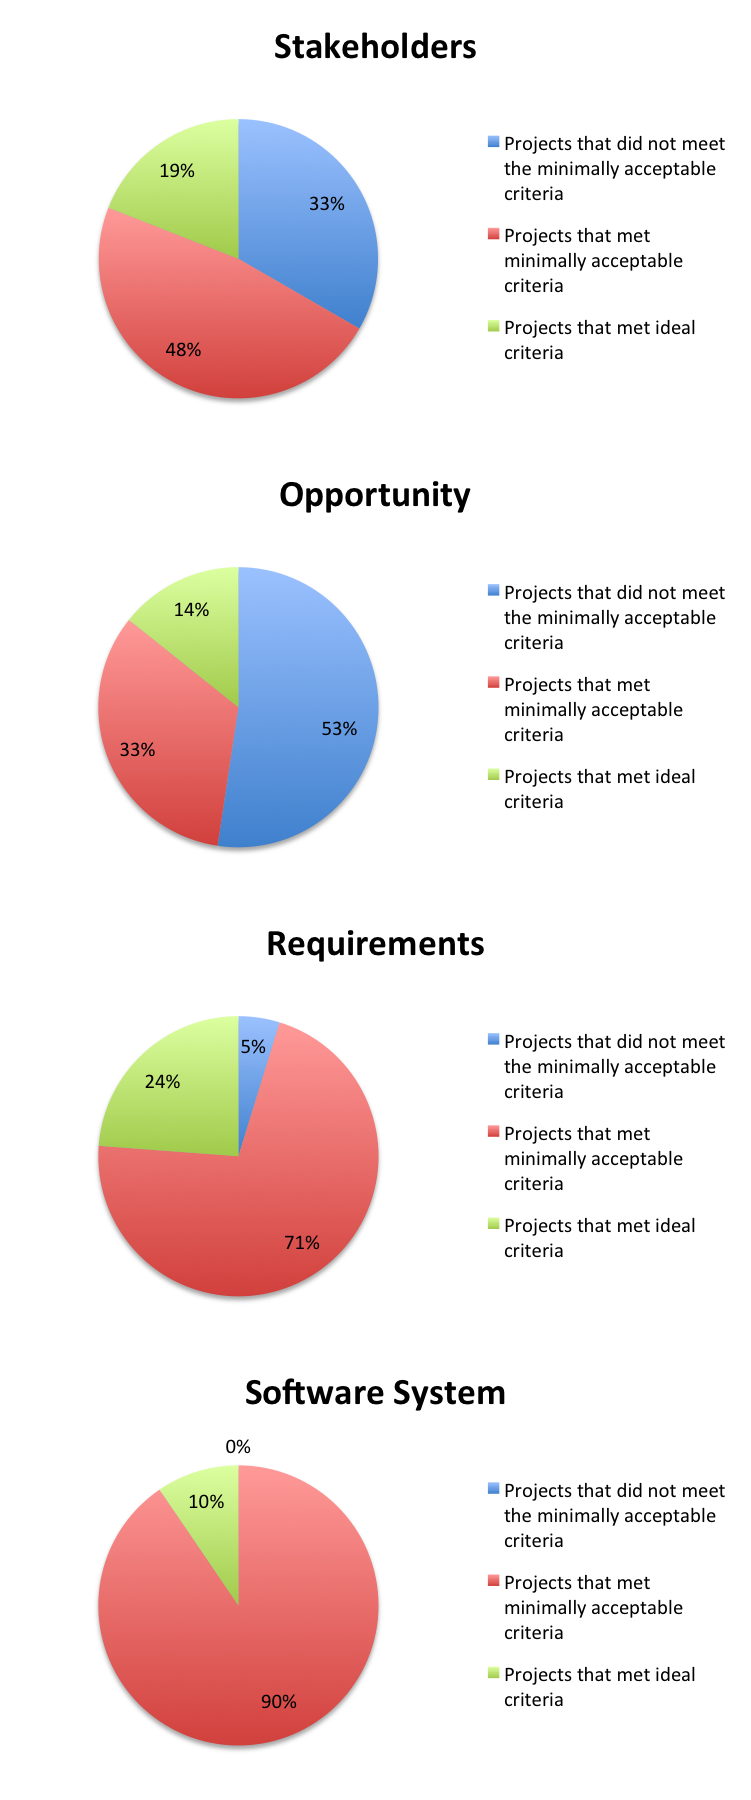
\includegraphics[width=3.45in]{essence_green_lighting_images/ProposalAlphasChartsStacked.png}
\caption{Essence Alphas checked for a proposal and circled for green-lighting project state}
\label{ProposalChart}
\end{figure}


In summary, we identified that 19\% of the proposals had represented
\textbf{Stakeholders}, 14\% of the proposals established the business value
of the \textbf{Opportunity}, 95\% \footnote{95\% is all the projects minus the 5\% that did not achieve any state} of the proposals captured the high level \textbf{Requirements} (and 24\% \footnote{24\% is the percentage of Bounded (19\%) and Coherent (5\%) projects} captured the project scope and success criteria), and 10\% of the proposals had defined criteria for selecting or identifying the \textbf{Software System} architecture. Since we do not expect the proposals to define architecture selection criteria, we are mostly concerned about the low
percentages for \textbf{Stakeholders} and \textbf{Opportunity} Alphas. Regarding
the \textbf{Requirements} Alpha, we would also like to increase the number of
proposals with defined project scope and success criteria.


\subsection{Research Question 2: What are some problems with the practicum that could potentially be mitigated to some extent prior to the start of the project?
}

While experimenting with Essence Reflection Meetings in the
context of practicum projects \cite{EASE2014, ICSE2014}, we
noticed that some practicum issues could potentially be identified and
addressed before the engagement started. These issues typically involve:

\begin{itemize}
\itemsep1pt\parskip0pt\parsep0pt
\item
  Missing stakeholder representation
\item
  Unclear opportunity value, and
\item
  Undefined project scope and success criteria
\end{itemize}

\textbf{Missing stakeholder representation:} Philosophical differences about
stakeholder representation present a challenge. The faculty believe that
most stakeholder groups should be represented and that a single
person cannot represent every stakeholder group because the groups
typically have very different needs. On one project, the team was building
a benchmark for comparing native code versus HTML5 code
on Android devices for the purpose of publishing the results to the
development community. While using the Essence framework for project
monitoring and steering \cite{ICSE2014}, the team
realized that no one represented the development community stakeholder
group. The team proactively interviewed local mobile developers and
presented the findings to the client. The client chose to ignore the
feedback putting at risk the potential benefit of the benchmarking
report to the development community. If a client is unwilling (or does
not understand the need) to have a representative for each (or most)
stakeholder groups, then the Request for Proposal process should
identify this issue and we can discuss our perspective with the client. If
the client is unwilling to change, we can decide to reject the
proposal.

\textbf{Unclear opportunity value and undefined project scope and success
criteria:} On a few projects, the teams spent the first two to three
weeks identifying the underlying problem and
analyzing the market trends and competitive landscape to validate the
need for a solution. Then they spent more iterations agreeing on the
project scope and success criteria. While this is an interesting
exercise, this significantly delayed the implementation work so the teams delivered substantially less functionality than the other
teams. Establishing the value of the opportunity and potentially
defining the project scope and success criteria at the start of the
practicum would have provided the practicum teams enough time to
build an interesting solution.

We believe that improving ``project readiness'' enhances the student experience, which remains to be verified in future research. If the stakeholder groups are not represented, then the
client can find representatives prior to the start of the project. If a client cannot clearly articulate the opportunity, the project's
benefits, the project's scope, or the project's success criteria, then
we can accept other proposals that have a larger impact.

Addressing these issues prior to the start of the practicum would
better align the expectations of the client with our educational goals, give the students a richer experience, provide more value to the client, and further the impact of the university.

\subsection{Research Question 3: From the faculty perspective, what should be the minimum or ideal initial state of a project?}

\begin{table*}
\renewcommand{\arraystretch}{1.3}
\caption{Green-lighting project state for each Essence Alpha (CMU1.1)}
\label{GreenLightingProjectState}
\begin{tabular}{|l|p{2.50in}|p{3.35in}|}
\hline
\textbf{Alpha}  & \textbf{Minimally acceptable}       & \textbf{Ideal}                        \\ \hline
Stakeholders    & \textbf{Recognized (Partial)}       & \textbf{Represented (Partial)}        \\ 
                & (check) Possible stakeholder groups are identified & (check) Stakeholder representatives are appointed \\
                & (not) Team agrees on relevant stakeholder groups & (check) Stakeholder representatives agree to take on responsibilities \\
                & to be represented                 & (not) Stakeholders agree on collaboration approach \\
                & (not) Responsibilities of stakeholder representatives  & (not) Representatives respect team's way of working \\
                & are defined                         & (check) Stakeholder representatives empowered to take on responsibilities \\ \hline
Opportunity     & \textbf{Solution Needed (Complete)} & \textbf{Value Established (Complete)} \\[5ex] \hline
Requirements    & \textbf{Conceived (Complete)}       & \textbf{Bounded (Partial)}            \\
                &                                     & (check) Purpose and extent of system are agreed \\
                &                                     & (check) Success criteria are clear \\
                &                                     & (not) Processes and tools for handling requirements are in place \\
                &                                     & (check) Scope constraints are identified \\
                &                                     & (not) Assumptions made while defining requirements are captured \\ \hline
Software System & None                                & \textbf{Architecture Selected (Partial)} \\
                &                                     & (check) Criteria for selecting architecture are agreed \\
                &                                     & (check) Platforms, technologies, languages are selected \\
                &                                     & (check) Selected architecture addresses key technical risks \\
                &                                     & (check) Buy, build, reuse decisions are made \\
                &                                     & (not) Stakeholders agree on necessary documentation \\
                &                                     & (not) Stakeholders agree on support service levels \\
                &                                     & (check) Non-functional architectural characteristics are considered \\ \hline
\end{tabular}
\end{table*}

After reviewing the practicum proposals and reflecting on practicum
issues listed in \textbf{Research Question 2}, we created green-lighting project
states for each Essence Alpha documented in Table~\ref{GreenLightingProjectState}.

The existing literature \cite{EssenceBook} implies
that staging (green-lighting in our case) can be done at the Alpha state level. In the process of creating our green-lighting project states, we discovered that for some of the Alpha states, we could not select all the checklist items in the entire state. For example, at the proposal stage, we do not expect responsibilities of the stakeholder representatives to be defined; this happens through a conversation between the team and the stakeholder representatives. In creating the green-lighting project state, we ignored some checklist items thus creating partial Alpha states.

The minimally acceptable and ideal states were defined with the goal of mitigating the problems identified in the previous research question, and based on the researchers expertise. Further work is necessary to validate the proposed states for each Alpha in the context of our practicum projects. Note however that other project courses might require different sets of minimally acceptable and ideal states to better address their specific needs.

\subsection{Research Question 4: How do the proposals
compare against the proposed minimum and ideal green-lighting project
states?}

Now that we have evaluated the proposals (Step 1) and created the
green-lighting project states (Step 2), we identify which proposals
meet the green-lighting criteria (Step 3 of the Green-lighting Approach). 

Table~\ref{table_proposal_evaluations} shows the proposals from the Spring 2014 and Summer 2014 semesters that meet the minimally acceptable and ideal criteria for green-lighting. 

\begin{table}
\renewcommand{\arraystretch}{1.3}
\caption{Proposals compared to green-lighting project states}
\label{table_proposal_evaluations}
\begin{tabular}{|p{1.10in}|p{0.95in}|p{0.95in}|}
\hline
Alpha & Number of projects that met minimally acceptable criteria & Number of projects that met ideal criteria \\ \hline
Stakeholders & 14 out of 21 & 4 out of 21 \\ \hline
Opportunity & 10 out of 21 & 3 out of 21 \\ \hline
Requirements & 20 out of 21 & 5 out of 21 \\ \hline
Software System & 21 out of 21 & 2 out of 21 \\ \hline
All (Satisfies all Alphas) & 8 out of 21 & 0 out of 21 \\ \hline
% Overall (Across all Alphas) & 8 out of 21 & 0 out of 21 \\ \hline
\end{tabular}
\end{table}

This analysis revealed a gap between the proposals and our
expectations, specifically in regard to representing stakeholders and
establishing the value of the opportunity. None of the proposals matched our ideal criteria across all Alphas, while 8 out of 21 satisfied our minimal expectation.

Around one third of the proposals did not have appropriate
representation for different stakeholder groups. In these proposals, the
client themselves would define, prioritize and validate the needs of the
different stakeholders groups. In our experience, when a team finishes
this kind of project, there is a high probability that the solution
would not deliver sufficient value for each stakeholders group. In some
cases, the solution may be unusable.

Around half of the proposals did not clearly state the
opportunity. The proposals described the problem to be solved, but did
not articulate the benefit of solving the problem. In a few cases, we
suspect the client has found a ``solution'' but has not yet identified
the problem to solve. In our experience, at the end of the project,
the project would be ``successful'' in delivering code to the client,
but might not solve a real world problem. Alternatively, the client
might have a detailed understanding of the opportunity, but may have not
clearly communicated that opportunity in the proposal.

The current proposals contain the same issues as the previous practicums identified in Research Question 2. The Green-Lighting Approach surfaced that the current proposals could repeat the problems identified in the past.


\subsection{Research Question 5: Do we need to
improve the Request for Proposal?}

In observing the gap between the proposals and our desired minimal
state, we wondered if asking different questions would help the sponsors
to record the kind of information that we need. Since the proposal's
content is a proxy for the sponsor's knowledge, is it possible that the
sponsor has more detailed knowledge that is not recorded in the proposal?
In addition, simply asking a question might cause the client to do some
groundwork not originally considered, which could potentially move the
project to a higher initial state. 

While analyzing the proposals, we had difficulty determining the stakeholder groups in the
 \textbf{Stakeholders} Alpha, the projected value of software system in the
 \textbf{Opportunity} Alpha, the list of high-level features that captures
the system purpose in the \textbf{Requirements} Alpha, and the non-functional
architectural characteristics in the \textbf{Software System} Alphas. The
Request for Proposal does not clearly ask for this information. We need
to ask specific questions to determine if the client can articulate the
answers. Improving the Request for Proposal would also facilitate
easier analysis for these aspects.

In order to help ascertain this information, we asked the sponsors four
questions.

{Survey Question 1. List your stakeholder groups and identify who will be
representing each group. (Note: Ideally there should be a different
person representing each group.)}

In examining the free-text answers, about \sfrac{2}{3} of the sponsors listed
out different stakeholder groups. A few even named who would fulfill the
role. One third of the sponsors listed themselves as the primary and
only stakeholder. In reviewing the proposals, these sponsors are not the
target stakeholder groups. This suggests that these proposals could be
misaligned with our educational goals of involving every stakeholder
group in the process.

{Survey Question 2. What value would the stakeholders receive from a successful engagement? If possible, please quantify the value (e.g. monetary
value, social return).}

In examining free-text answers, about half of the respondents were not
able to articulate the opportunity of the proposal. The other half of
the respondents appealed to social returns such as improving the
emergency response situations which could save lives and reduce injuries
or connecting seniors to their families and caregivers. None of the
respondents were able to put a monetary value to the opportunity.

{Survey Question 3. What features would you like to see implemented during the
practicum? }

In reviewing the free-text answers, about half of the sponsors provided
a feature list. The other half provided vague answers to the question.
This question needs to be rephrased. Perhaps asking the client to
prioritize the features to be delivered would be more effective.

{Survey Question 4. What are the key non-functional requirements (e.g.
scalability, security, performance, etc) that the solution should
satisfy?}

Most of the sponsors were able to clearly articulate the quality
attributes needed for the project. One sponsor said, ``Software will be
written in C/C++, documented well and reusable.'' 

When the answer does not fully or properly articulate the
non-functional requirements of the system, we recommend that the course
owner interviews the sponsor to acquire this information. 

The results from questions 1 and 2 are consistent with our assessment
of the proposals from Research Question 1. Adding these questions would
facilitate analysis but might not cause the sponsors to change the
stakeholder representation. Additional conversations between the course 
owner and the sponsor might be necessary.

Based upon these results, we plan to add questions 1, 2, and 4 to our
Request for Proposal. We will continue to experiment to find a question
that elicits a list of high-level features. These improvements to
our Request for Proposal will help us better assess the initial states
of the proposals.

% \subsection{Research Question 6: What is the effect of
% using the Essence Green-lighting Approach on the time it takes to accept
% or reject a project?}

% With modifications to the Request for Proposal questions, we believe
% that the Essence Green-lighting Approach would structure, simplify, and
% reduce the amount of time it takes to accept or reject a proposal when compared to our current process.
% However this remains to be verified.

In the current Request for Proposal process, the course owner reads
through each proposal to verify its completeness. We noticed that
clients submit ad-hoc proposals without necessarily following the
provided guidelines in terms of structure and content. This makes
assessing the readiness of each proposal arduous. The Request for
Proposal process provides a non-editable document and asks the sponsor
to address the items listed in Section
\ref{ProposalQuestions}. We recommend replacing this
document with a restructured editable template where the sections are
clearly aligned to the four Essence Alphas. Clients would be asked to
fill-in the sections of this template. 

% With the proposed Green-lighting Approach, the course owner still needs
% to read through each proposal, but instead of looking for completeness,
% the course owner assesses the four Essence Alphas in the green-lighting
% project state. This requires the small additional effort of reading
% through at most 23 checklist items, and even less if the proposals are
% less mature. These changes would reduce the time on task for the current
% verification for completeness of ad-hoc proposals by organizing the data
% provided by the client and simplifying the assessment of the
% green-lighting project states.

\subsection{Research Question 6: What are limits to
the approach and limitations to its effectiveness?}

\subsubsection{Green-lighting Approach does not factor important business considerations}
The approach provides data for a structured decision making process for
accepting and rejecting proposals, however, there might be reasons to
have a project go forward even though green-lighting says ``no.''
Several examples include paying clients, a high impact project, career
opportunity for students, and potential partnership for research
collaboration. While the approach provides a black and white answer,
we suspect that sound judgment is required for special circumstances.

\subsubsection{Green-lighting project states do not always
align to Alpha states}

In following the Green-lighting Approach, we discovered that partial
states, not Alpha states, represent our proposal acceptance criteria.
Some of the checklist items on one Alpha state would apply to accepting
a proposal and the rest of the checklist items would not. For example, 
for us to green-light a proposal, we would expect that the
proposal would meet the first checklist item of the
 \textbf{Stakeholders} \textit{Recognized} card, not the second or third as
described in Table \ref{GreenLightingProjectState}. 
Using partial states is possible but inconvenient. 

\subsubsection{Green-lighting Approach relies upon the Essence framework}
The Green-lighting Approach relies upon the Essence kernel for providing 
a systematic framework for evaluating proposals. The case study shows that  
only a subset of the framework is leveraged: Only 4 out of the 7 Alphas are 
relevant, and only the first few states (maximum 3) of each Alpha are necessary 
to green-light a project. In addition, some of the states need to be only partially 
considered as described in the previous section. Therefore, it is possible that a simpler checklist 
could be evolved, rather than relying upon the Essence framework. The extra 
complexity could be justified however if the project team continues to use 
the Essence framework during development to leverage mechanisms like progress 
monitoring and project steering. In that case it might make sense to use the 
same framework throughout the project.

\subsubsection{Green-lighting Approach does not guarantee project success}
Given the variety of issues that can emerge from a student project experience, and the fact that the initial state has only a limited impact on the overall project, the Green-Lighting Approach is not a silver bullet that will solve all team-based issues.
Only some risks might be reduced by systematically examining each proposal to identify
potential problems that the instructor could solve, mitigate against, 
or simply decide not to deal with by rejecting the proposal.

\subsection{Threats to Validity}
Internal Validity: This work assumes that it is desirable to filter
proposals and that is is possible to select proposals that will better achieve the
practicum goals listed in Section \ref{Introduction}. It could be the case
that a rejected proposal would have more significant learning
opportunities for the students than an accepted proposal.

Experimenter bias: We each had one years worth of experience in working with
the Essence framework prior to the start of this research. It is
possible that someone with less experience may encounter different results.

\section{Conclusions and Future Work}
\label{Conclusion}

This paper presents a first attempt to characterize and study a project 
selection process in academia. We proposed a Green-lighting Approach using the Essence framework and
applied the approach to the Request for Proposal process for the
practicum course at Carnegie Mellon University in Silicon Valley. 

After receiving and reviewing a set of proposals, the faculty determined each 
proposal state for each Essence Alpha. Based upon these initial states, prior experience, 
and recent problems, we created a gating function called green-lighting project
state to screen out proposals that are not ready for student teams.

After creating the green-lighting project state for each
Essence Alpha, we realized that our current Request for Proposal did
not prompt the clients to provide enough detail about the stakeholder
representations, the projected value of the opportunity, the project
scope and success criteria, and non-functional architectural
characteristics of the software system. We created draft 
questions and then tested the new questions with the prospective
clients. We recommend modifying our Request for Proposal to include
an editable template structured around the Essence Alphas and to include
several of the new questions identified in this paper. 

Further research is necessary to validate our green-lighting project state 
as well as our modified Request for Proposal. 
Even though green-lighting projects does not guarantee project success, 
the goal is to reduce risks by systematically examining each proposal to identify
potential problems that the instructor could solve, mitigate against, 
or simply decide not to deal with by rejecting the proposal.
More work is necessary to verify that our approach helps us reach that goal.

Using the Essence framework for green-lighting practicum projects in academia presents some limitations. 
First, the approach does not explicitly factor in business forces that affect proposal selection. 
Second, the Essence framework might be overly complex for green-light practicum projects, 
as only a subset of the Essence framework is necessary to perform the task.
In addition, the need to split the checklist items on the Alpha states to represent green-lighting 
project states prevents us from using the Essence cards out of the box hence losing the simplicity of the cards.

Still, project courses that use the Essence framework during development (to leverage mechanisms such as progress 
monitoring and project steering \cite{ICSE2014}) might want to borrow some ideas from the proposed Green-Lighting Approach, 
as it might make sense to leverage the same framework throughout the project.
In that case, we recommend customizing the approach by defining minimally acceptable and ideal states based on the course specific needs. 

For project courses that are not planning on using Essence during development, 
the framework could still be used as an inspiration for deriving simple custom green-lighting checklists for various project dimensions. Better aligning client proposals and educational goals has the potential of enhancing the students learning experience.


% % \begin{table}[h]
% \centering
% \renewcommand{\arraystretch}{1.5}
% \caption{Concise comparison of Grounded Theory Approaches}
% \label{ConciseGroundedTheoryComparison}
% \begin{tabular}{|p{1.3in}|p{1.5in}|p{1.5in}|p{1.5in}|}
% \hline
%                                     & Classic Grounded Theory                                                                              & Straussian Grounded Theory                                  & Constructivist Grounded Theory                                                                      \\ \hline
% The influence of research questions & emerges from the research                                                                            & may be defined upfront                                      & may be defined upfront and evolves through study                                                    \\ \hline
% The role of existing literature     & delays use of literature in the process                                                              & use when needed                                             & use when needed                                                                                     \\ \hline
% Analytic coding                     & Theoretical Coding                                                                                   & Axial Coding                                                & Theoretical Coding                                                                                  \\ \hline
% Analytic questions                  & \quotes{what is this data a study of?}                                                             & hypothesizing as to causes of the data                      & \quotes{what is this data a study of?}                                                            \\ \hline
% Philosophical differences           & objectivism                                                                                          & pragmatism                                                  & social constructionism                                                                              \\ \hline
% Evaluation criteria                 & fits the data, works in explaining main concern, relevance to participants, modifiable with new data & Seven criteria for process and eight criteria for grounding & credibility (enough data), originality, resonance with participants, usefulness with intepretations \\ \hline
% \end{tabular}
% \end{table}

\chapter{Practice and Perception of Team Code Ownership}
\section{TeamCodeOwnership}

\textit{Context:} Team code ownership is a software development practice where any team member can modify any part of the team's code. However, many factors beyond official policy affect a developer's sense of ownership. 

\textit{Objective:} The purpose of this paper is to understand the factors that affect a team's sense of code ownership.

\textit{Method:} Following Constructivist Grounded Theory, the first author conducted participant-observation of several software development projects, and interviewed 21 software engineers, interaction designers, and product managers. Iterating between theoretical sampling and analysis continued until achieving theoretical saturation.

\textit{Results:} Team code ownership is a feeling. Developers feel team code ownership more when they understand the system context, have contributed to the code in question, perceive code quality as high, believe the product will satisfy the user needs, and perceive high team cohesion.  

\textit{Limitations:} Outcomes of grounded theory research are not statistically generalizable to defined populations, and may not apply to organizations with different software development cultures.

\textit{Conclusion:} Team code ownership is rooted in numerous cognitive, emotional, contextual and technical factors and cannot be achieved simply by policy. 

\section{Introduction}
\textit{Team Code Ownership} (which is similar to \textit{Collective Code Ownership} and \textit{Shared Code}) is a software development practice where any developer on a team has the right to change any of the team's code. Team code ownership is intended to accelerate development by allowing any developer to fix any team bug and by mitigating delays due to vacations, illness and other absence \cite{BeckExtremeProgramming2004}.
 
While some research has investigated the effects of different code ownership models, we are unaware of any studies that specifically investigate developers' sense of team code ownership; that is, the complex interactions between developers' knowledge, emotions, and approach to code ownership.  

When team code ownership emerged as a core category in a grounded theory study, we therefore exploited this opportunity to investigate factors associated with perceived code ownership and related phenomena. 

We quickly discovered that having the right to change a file does not mean that a specific developer will feel empowered to and justified in making a specific change. For example, a developer may feel reluctant to change code that he or she does not really understand. As we refined this core finding and allowed it to drive further data collection, we identified five factors associated with feelings of team code ownership. 

This paper consequently reviews existing research connected to team code ownership (Section \ref{RelatedWork}), describes our grounded theory approach (Section \ref{ResearchMethod}), and presents our emerging results: five factors associated with team code ownership (Section \ref{TeamCodeOwnership}). Section \ref{Discussion} discusses the study's implications and limitations, followed by a summary of its contributions (Section \ref{Conclusion}).
\section{Related Work}
\label{RelatedWork}

\subsection{Team Code Ownership}
In Extreme Programming \cite{BeckExtremeProgramming2004}, Kent Beck describes a set of interdependent practices for managing feature development and facilitating a collaborative team environment. One of these practices is \textit{collective ownership}---\quotes{Anyone can change any piece of code in the system at any time.} \cite{BeckExtremeProgramming2000}. The book contrasts collective ownership against \quotes{no ownership} and \quotes{individual ownership.} In 2004, collective ownership is renamed \textbf{shared code} \cite{BeckExtremeProgramming2004}.

In 2006, Martin Fowler defined \textit{collective code ownership}, similarly to Beck \cite{FowlerCodeOwnership}, as a contrasting team position to \quotes{strong code ownership} where each file has one owner and \quotes{weak code ownership} where developers can change files, but an owner keeps an eye on files for which they are responsible. 

Later, Bird et al. \cite{BirdDontTouchMyCode} contrasted the effects of strong- and weak-ownership. They demonstrated that weak ownership leads to more defects than strong ownership for Windows Vista and Windows 7. The study defined ownership for a software component as a percentage of the version control commits for a single developer. They defined a major contributor as someone who has more than 5\% of the git commits. A sensitivity analysis revealed that defining strong code ownership within the range from 2\% to 10\% produced similar results for the study.

Meanwhile, Murphy  \cite{MurphyIEEESoftware} argued that the concept of code ownership must be unpacked and expanded. He argued that the complexities of code ownership are missed by merely examining git commits to determine who modified which files.

Our paper renames \textit{collective code ownership} to \textit{team code ownership}. For small systems and teams, these terms are synonymous. For a large system with multiple teams, in practice, teams would have strong ownership of their portion of the system. Allowing any pair to modify any part of Microsoft Windows or Pivotal Cloud Foundry is impractical.

Team code ownership requires more than a team saying, \quotes{everyone can modify anything.} Instead, this paper examines how a team feels that they own the code. We define \quotes{sense of team code ownership} as the degree to which individual members of the team feel collective ownership.  

\begin{table*}[t]
\renewcommand{\arraystretch}{1.5}
\centering
\caption{Theory of Sustainable Software Development: Principles, Policies, and Practices}
\label{SustainableSoftwareDevelopmentTable}
\begin{tabular}{|p{2.5in}|p{3.4in}|}
\hline
\multicolumn{2}{|c|}{Sustainable Software Development}              
\\
\hline
Underlying Principles & Keeping a Positive Attitude Toward Team Disruption \newline Encouraging Knowledge Sharing and Continuity \newline Caring about Code Quality \\ 
\hline
Policies & Team Code Ownership \newline Shared Schedule \newline Avoid Technical Debt  \\
\hline
Removing Knowledge Silos Practices & Continuous Pair Programming \newline Overlapping Pair Rotation \newline  Knowledge Pollination  \\
\hline
Caretaking the Code Practices & TDD / BDD \newline Continuous Refactoring  \newline Supported by Live on Master \\
\hline
\end{tabular}
\end{table*}

% \begin{table*}[t]
% \renewcommand{\arraystretch}{1.5}
% \centering
% \caption{Theory of Sustainable Software Development: Principles, Policies, and Practices}
% \label{SustainableSoftwareDevelopmentTable}
% \begin{tabular}{|p{1.65in}|p{1.35in}|p{1.8in}|p{1.6in}|}
% \hline
% \multicolumn{4}{|c|}{Sustainable Software Development}                     \\
% \hline
% Underlying Principles & Policies                  & Removing Knowledge Silos Practices & Caretaking the Code Practices       \\
% \hline
% $\bullet$ Keeping a Positive Attitude Toward Team Disruption & $\bullet$ Team Code Ownership & $\bullet$ Continuous Pair Programming         & $\bullet$  TDD / BDD                   \\
% $\bullet$ Encouraging Knowledge Sharing and Continuity & $\bullet$ Shared Schedule           & $\bullet$ Overlapping Pair Rotation & $\bullet$ Continuous Refactoring      \\
% $\bullet$ Caring about Code Quality  & $\bullet$ Avoid Technical Debt      & $\bullet$  Knowledge Pollination    & Supported by Live on Master \\ 
% \hline
% \end{tabular}
% \end{table*}


\subsection{Sustainable Software Development}
\label{SustainableSoftwareDevelopmentTheory}
We describe the theory of Sustainable Software Development through Overlapping Pair Rotation in the paper by the same name \cite{SustainableSoftwareDevelopment} and summarize it in Table \ref{SustainableSoftwareDevelopmentTable}. The theory describes how teams can continue to deliver value in spite of team disruptions. The theory is a collection of synergistic principles, policies, and practices encouraging a positive attitude towards team disruption, knowledge sharing and continuity, as well as caring about code quality. The practices actively remove knowledge silos and caretake the code so that any pair can work on any story in the backlog. 

\subsection{Psychological Ownership}
Psychological ownership refers to \quotes{the feeling of possessiveness and of being psychologically tied to an object} \cite{Pierce2001}. Targets of ownership, whether physical or immaterial, become the extension of one's self: \quotes{What is mine becomes (in my feelings) part of ME} \cite{Isaacs1933}. Ownership can be attached to a part or the whole. Psychological ownership occurs when the object becomes part of the psychological owner's identity. Psychological ownership answers the question, \quotes{What do I feel is mine?}

Changes in ownership can have strong effects on our self-identity. An increase in the number of possessions can produce positive effects \cite{Formanek1994}, while a diminish can lead to a personality shrinkage \cite{James1890}. Someone threatening a person's ownership can trigger strong emotions and responses.

Peirce \cite{Pierce2001} identifies three sources or \quotes{roots} of psychological ownership: efficacy and effectance, self-identity, and having a place. A major reason for possession of physical goods or abstract ideas is rooted in the innate human desire to be in control; being able to alter one's environment creates feelings of efficacy and pleasure. Ownership fulfills the need for self-identification as people define themselves, express themselves, and ensure their own survival by what they own. Ownership fulfills the need to have a place and a territory to possess. \quotes{Each motive facilitates the development of psychological ownership, rather than directly causes this state to occur.} Psychological ownership occurs with code because creating software can satisfy the desire for efficacy and effectance, self-identity, and having a place.

Peirce identifies three paths or \quotes{routes} to ownership: controlling the target, coming to intimately know the target, and investing the self into the target. With \emphasis{controlling the target}, targets that can be controlled are perceived to be part of the self.  As  individuals repeatedly exercise control of an object, eventually this leads to \quotes{feelings of ownership toward that object.} The higher the autonomy of the job task, the more likely ownership develops toward the activity. When a person has little control over an activity, psychological ownership is unlikely to develop. With \emphasis{coming to intimately know the target}, the association with the object creates feelings of ownership. One example is when a gardener feels that the garden belongs to the gardener. (This happens routinely with software developers who feel that they own part of the code base, when in reality, the company owns the software.) Feelings of ownership increase as one becomes intimately familiar with the object and associated with it. With \quotes{investing the self into the target,} we feel that we own what we create, shape or produce. Spending time, energy, and effort enables us to alter our view of ourselves to include identity with the object. The more investing in the object, the stronger the psychological ownership. Nonroutine, complex jobs infuse more of our own ideas resulting in increased ownership.

\section{Research Method}
\label{ResearchMethod}

\subsection{Constructivist Grounded Theory}
We followed Charmaz' approach to Grounded Theory \cite{Charmaz}, which provides an iterative approach to data collection, data coding, and analysis resulting in an emergent theory. The two primary data sources were field notes collected during continuous participant observations of a 7.5-month project and interviews with 21 Pivotal software engineers, interaction designers, and product managers. Interviews were recorded, transcribed, coded, and analyzed using constant comparison. Our presentation is informed by Stol et al.'s reporting guidelines for grounded theory studies in software engineering \cite{StolGTinSE}. 

When starting a grounded theory research study, the core question is \quotes{What is happening here?} (Glaser, 1978) \cite{GlaserTheoreticalSensitivity}. Our initial core question was: \quotes{What is happening at Pivotal when it comes to software development?} This question led to the Theory of Sustainable Software Development summarized in Section \ref{SustainableSoftwareDevelopmentTheory}. When team code ownership emerged as one of the core categories of the theory, the researcher collected additional data in order to identify the factors affecting the sense of code ownership. The factors are introduced in Section \ref{TeamCodeOwnership} and are the main contributions of the paper.

\subsection{Data Collection}
The primary researcher relied on \quotes{intensive interviews,} which Charmaz summarizes as \quotes{open-ended yet directed, shaped yet emergent, and paced yet unrestricted} \cite{Charmaz}. The technique relies on open-ended questions. The purpose is for the researcher to enter into the participant's personal perspective within the context of the research question. 

While exploring new emergent core categories, whenever possible, the researcher initiated subsequent interviews with a goal of not forcing the issue. For example, \quotes{please draw your feelings about the code} often resulted in conversations about code ownership. After the interview, the interview was transcribed into a Word document with timecode stamps for each segment.

The primary researcher collected field notes while working as an engineer. The field notes comprise multiple paragraph entries recorded several times a week collected over a six month period. The notes describe individual and collective actions, captures what participants defined as interesting or problematic, and include anecdotes and observations. 

\subsection{Research Context: Pivotal}
\label{ResearchContext}
Pivotal is a large American company with 16 offices around the world. One of its divisions is Pivotal Labs. Pivotal Labs' mission is to both deliver highly-crafted software products and provide a transformative experience for their client's engineering cultures. To change a developer's way of working, Pivotal combines the client's software engineers with Pivotal's engineers at a Pivotal office where they can experience Extreme Programming in an environment conducive for agile development. % Tmp for 6 pages    For startups, Pivotal might be the first engineers working on the project. For enterprise clients, Pivotal provides additional engineering resources to accomplish new business goals. 

A common team size is six developers plus an interaction designer and a product manager. In the history of the Palo Alto office, the number of developers on a project ranges from 2 to 28. Larger projects are organized into smaller coordinating teams with one product manager per team and one or two interaction designers per team.

% Tmp to fit in 6 pages
%Commonly utilized technologies include Angular, Android, Backbone, iOS, Java, Rails, React, and Spring which are often deployed onto Pivotal's Cloud Foundry. 

Pivotal Labs has followed Extreme Programming \cite{BeckExtremeProgramming2004} since the late 1990s. While each team is autonomous in making its own decisions as to what is best for a particular project, the company culture strongly suggests following all of the core practices of Extreme Programming. % Tmp to fit in 6 pages  This includes Pair Programming, Test Driven Development, Weekly Retrospectives, Daily Stand-ups, Prioritized Backlog, Whole Team ownership of the project and code base, plus Kanban's notion of work flowing through people.

\section{Team Code Ownership}
\label{TeamCodeOwnership}

In the literature, collective code ownership is often treated as a policy statement. In this case, simply claiming that \quotes{anyone can modify any piece the code} was not sufficient to engender willingness to modify any file. Rather, ownership is an emotional or qualitative attribute that ties all developers on the team to the project and code base. It is a spectrum where, on one side, each individual has ownership of only their code, and on the other side, everyone on the team owns the entire code base. Some events appear to erode the team's sense of ownership over the project's duration, while some practices appear to counteract these erosions. This section details the five factors that appear most related to team code ownership and examples of events or tendencies that erode it. 

% \begin{table*}[]
% \renewcommand{\arraystretch}{1.5}
% \centering
% \caption{Factors affecting Team Code Ownership}
% \label{TeamCodeOwnerhipFactors}
% \begin{tabular}{|p{1.3in}|p{2.6in}|p{2.6in}|}
% \hline
% Factor & Definition & Purpose \\
% \hline
% System Context
% & System context is the knowledge and situational awareness about the code, including the discourse that surrounds the code. %System context includes understanding how existing features have been implemented, understanding existing design decisions, understanding underlying technologies and frameworks, and understanding how features solve the user's need.
% & Developing a deep knowledge of the system exercises the \quotes{intimately knowing the target} path of psychological ownership.
% \\ \hline
% Code Contribution
% & Code contribution is the portion of the code that a given developer has worked on.
% & Personally contributing to the code base increases a developer's sense of ownership by exercising \quotes{investing in the target} path of psychological ownership. % As a developer works on the code base, the developer's system context level increases. While code contribution level influences the system context level, it is not necessary related: developers might learn about the code through other means different from direct contribution, including conversations at stand-up, impromptu team huddles, or a pair saying \participantQuote{Check out what we did yesterday.}
% \\ \hline
% Code Quality
% & Code quality relates to how well the code satisfies the project's desirable quality attributes. Desirable quality attributes might include design qualities, performance, reliability, scalability, security,  testability, and usability \cite{Meier2009}.
% & %How well the code satisfies the project's desirable quality attributes affects the team's sense of ownership. 
% A high quality product satisfies the self-identity motivation of psychological ownership. Developers might not want to be identified with a low quality product.
% %Low quality products also tend to involve a disproportionate amount of bug fixes. Developers need a balance between creating new features and fixing bugs each week. Working only on bugs for weeks affects their sense of ownership.
% \\ \hline
% Product Fit
% & Product fit is believing that the product will satisfy the user's needs.
% & Engineers want to create products that matter to the user. Delivering a product that matters to someone satisfies the self-identity motivation of psychological ownership.
% \\ \hline
% Team Cohesion
% & Team cohesion is the degree to which team members identify as part of the team, stick together through adversity and take pride in the team's accomplishments \cite{Bollen1990Perceived, Beal2003Cohesion, Whitworth2007Motivation}.
% & Team cohesion satisfies the \quotes{having a place} motivation of psychological ownership.
% \\ \hline
% \end{tabular}
% \end{table*}




% (Table \ref{TeamCodeOwnerhipFactors}). 





% \begin{table}[]
% \renewcommand{\arraystretch}{1.5}
% \centering
% \caption{Factors affecting Team Code Ownership}
% \label{TeamCodeOwnerhipFactors}
% \begin{tabular}{|p{3.1in}|}
% \hline
% System Context \\
% Code Contribution \\
% Code Quality \\
% Product Fit \\
% Team Cohesion \\
% \hline
% \end{tabular}
% \end{table}

% \begin{landscape}
% % \begin{sidewaystable}
% \begin{table}[]
% \renewcommand{\arraystretch}{1.5}
% \centering
% \caption{Factors affecting Team Code Ownership}
% \label{TeamCodeOwnerhipFactors}
% \begin{tabular}{|p{1.3in}|p{2.5in}|p{2.5in}|p{2.5in}|}
% \hline
% Factor & Definition & Purpose & Threats \\
% \hline
% System Context
% & System context is the knowledge and situational awareness about the code, including the discourse that surrounds the code. System context includes understanding how existing features have been implemented, understanding existing design decisions, understanding underlying technologies and frameworks, and understanding how features solve the user's need.
% & Developing a deep knowledge of the system exercises the \quotes{intimately knowing the target} path of psychological ownership.
% & Increasing code base size; Increasing team size
% \\ \hline
% Code Contribution
% & Code contribution is the portion of the code that a given developer has worked on.
% & Personally contributing to the code base increases a developer's sense of ownership by exercising \quotes{investing in the target} path of psychological ownership. As a developer works on the code base, the developer's system context level increases. While code contribution level influences the system context level, it is not necessary related: developers might learn about the code through other means different from direct contribution, including conversations at stand-up, impromptu team huddles, or a pair saying \participantQuote{Check out what we did yesterday.}
% & Inability to contribute
% \\ \hline
% Code Quality
% & Code quality relates to how well the code satisfies the project's desirable quality attributes. Desirable quality attributes might include design qualities (e.g. conceptual integrity, maintainability, reusability, discoverability), run-time behavior (e.g. availability, interoperability, manageability, performance, reliability, scalability, security), system qualities (e.g. supportability, testability), and user qualities (e.g. usability) \cite{Meier2009}.
% & How well the code satisfies the project's desirable quality attributes affects the team's sense of ownership. When a product does not achieve an acceptable quality level, a developer may not want to be identified with the product and thus the self-identification motivation of psychological ownership is not being met. Low quality products also tend to involve a disproportionate amount of bug fixes. Developers need a balance between creating new features and fixing bugs each week. Working only on bugs for weeks affects their sense of ownership.
% & Pressure to deliver and deprioritizing continuous refactoring
% \\ \hline
% Product Fit
% & Product fit is believing that the product will satisfy the user's needs.
% & Engineers want to create products that matter to the user. Delivering a product that matters to someone satisfies the self-identity motivation of psychological ownership.
% & Ignoring developers feedback about the product
% \\ \hline
% Team Cohesion
% & Team cohesion is the degree to which team members identify as part of the team, stick together through adversity and take pride in the team's accomplishments \cite{Bollen1990Perceived, Beal2003Cohesion, Whitworth2007Motivation}.
% & Team cohesion satisfies the \quotes{having a place} motivation of psychological ownership.
% & Distancing a developer from the team
% \\ \hline
% \end{tabular}
% \end{table}
% \end{landscape}

%\begin{figure}[t]
%\centering
%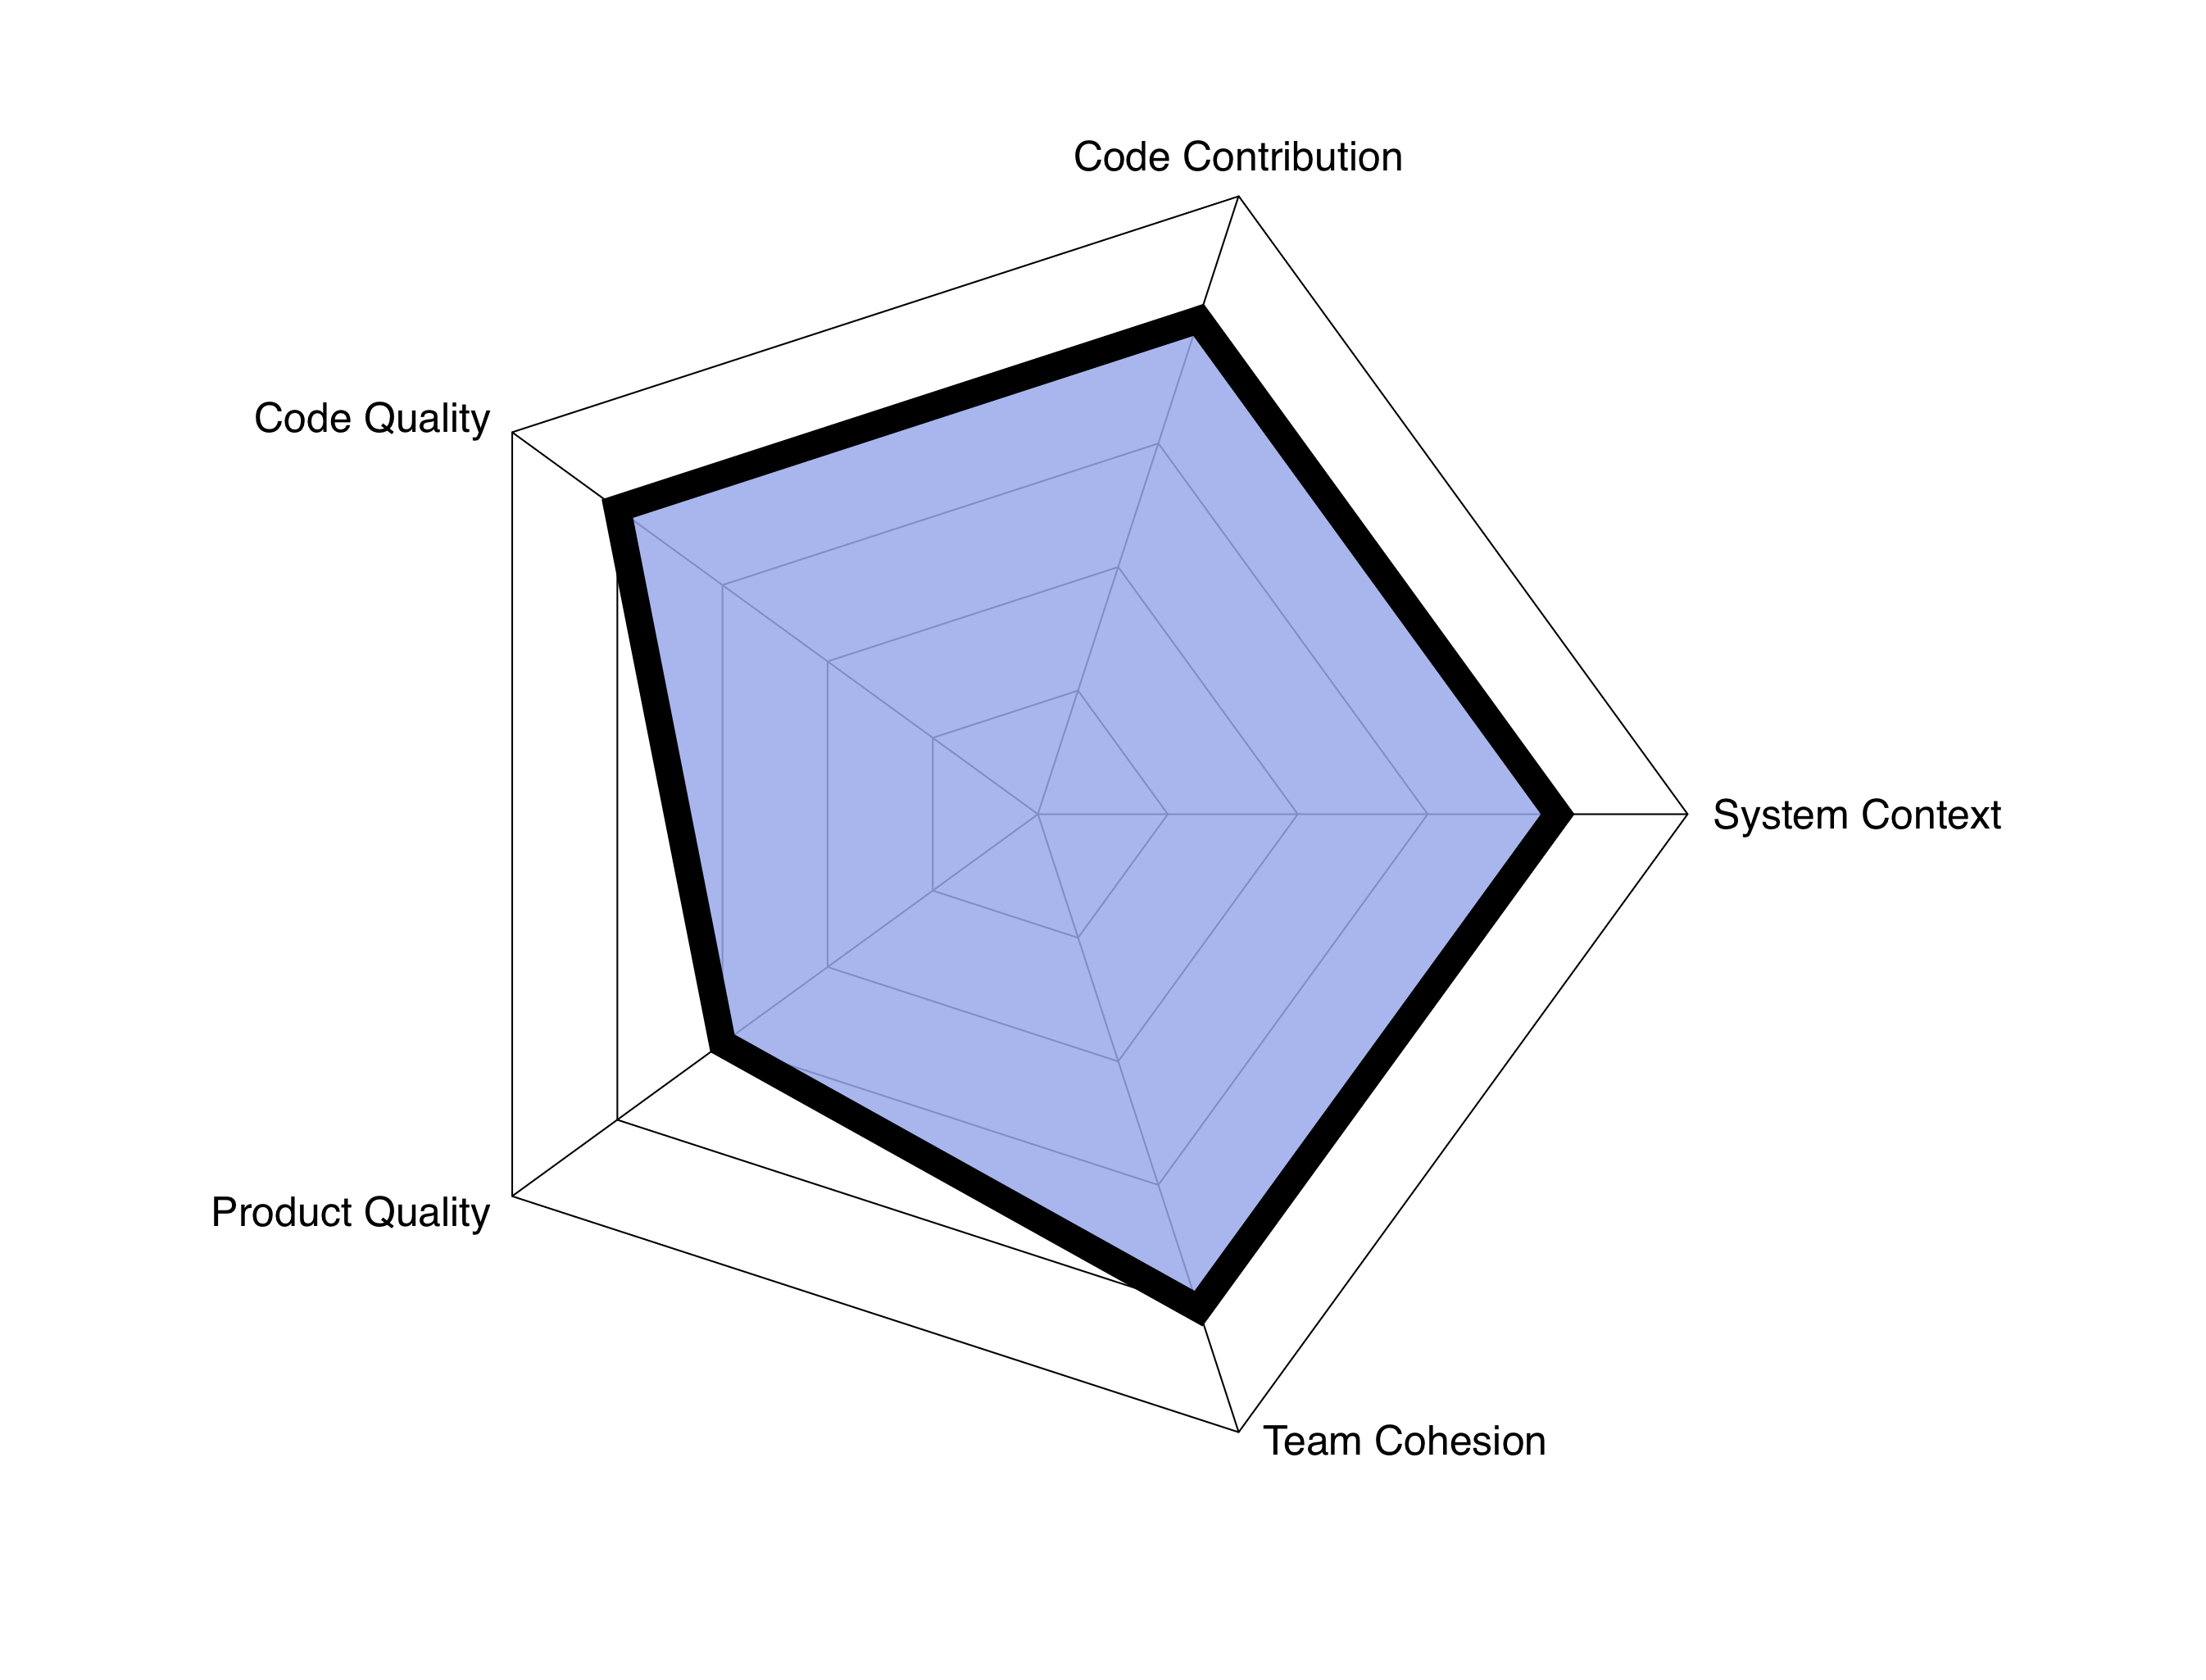
\includegraphics[width=3.45in]{team_code_ownership_images/Spider.png}
%\caption{Spider chart illustrating the factors of team ownership}
%\label{TeamOwnershipSpider}
%\end{figure}

\subsection{System Context}
\textbf{Definition:} System context is the knowledge and situational awareness about the code, including the discourse that surrounds the code. System context includes understanding existing design decisions, underlying technologies, the relationship between features and user needs, and the implementation of existing features.

\textbf{Purpose:} Developing an in-depth knowledge of the system exercises the \quotes{intimately knowing the target} path of psychological ownership.

For a pair to work efficiently on any part of the system, one of them needs to have enough context to know how that part of the system works. Without enough context, a pair might struggle, slow down, or be blocked in working on a feature.

Code ownership seems to vary with the context that the developer has about the code; the more the developer knows, the higher the sense of ownership. Knowledge silos, the size of the code base, or the number of developers working in parallel can make it difficult for a programmer to develop a deep system context level.

\textbf{Threat: Increasing knowledge silos.} When developers routinely work on one part of the code base, they can develop specific system context not shared by the team. Code specialization impedes anyone on the team from modifying any part of the team's code.  One team said \participantQuote{We need Marion on that story, only she knows the Apple watch code base,} and \participantQuote{Shea knows the ins-and-outs of the legacy integration, we need him to work on this story,} which means there is a hindering imbalance between the individual and team understanding of the code.

\textbf{Threat: Increasing code base size.} The primary researcher participated on a team working with a large code base that was over eight years old and the team did not have a full understanding of the system. Initially, the team felt little ownership of the code, even though the team was responsible for it and agreed to \singleQuote{team code ownership.} Often the team would need to ask a product manager why certain features exist in the code to understand the code's purpose and implementation. In time, as the team worked with the code and gained context, the team's sense of ownership improved.

\textbf{Threat: Increasing team size.} The primary researcher observed the relationship between team size and code context on five Pivotal projects as a participant-observer. As team size increases, the ability to gain system context decreases. Every day, all pairs are adding to the system. On a five pair team, so much work is happening each day that it becomes increasingly difficult to keep track of everything that changes.

One developer on a ten-person project said, \participantQuote{I feel that we don't have the context spread around fully. Having five, sometimes six, pairs on the project makes it go really fast, so it's hard to keep context.}

When developers do not have context about part of a system, or context about what remains to be done to finish a story, reluctance to start the next story at the top of the backlog emerges. It's easier to start a story that touches part of the system that they know. As one developer reflected, \participantQuote{I am not entirely comfortable to jump into stories on certain aspects [of the system].}

As a coping strategy, one developer, before the start of the work day, skimmed the git commits from the previous day to learn about new classes and changes in design and to understand the features the team added. 

As team size grows, there is a potential risk of decreasing an individual developer's sense of team code ownership. 

\subsection{Code Contribution}
\textbf{Definition:} Code contribution is the portion of the code that a given developer has worked on. 

\textbf{Purpose:} Personally contributing to the code base increases a developer's sense of ownership by exercising \quotes{investing in the target} path of psychological ownership. 

As a developer works on the code base, the developer's system context level increases. While code contribution level influences the system context level, it is not necessary related: developers might learn about the code through other means different from direct contribution, including conversations at stand-up, impromptu team huddles, or a pair saying \participantQuote{Check out what we did yesterday.}

\textbf{Threat: Inability to contribute.}  A developer's inability to contribute to the code base decreases the developer's sense of ownership. 

This could happen, for instance, during a pair programming breakdown. When the pairing experience breaks down, one person drives the code development while the partner passively watches. (We call this dynamic \quotes{Performance Pair Programming,} when one developer plows through a story and stops listening to the developer's partner.)  When one person is writing all the code, individual code ownership replaces team code ownership.  

%six paper vesion
In one situation, the partner took over and ignored the participant's input. The participant reflected, \participantQuote{I would not be able to explain deeply what we had done. I would not be able to maintain it. I didn't really write it, so I feel very little ownership of it.} 

% full version: In one situation, the partner took over and ignored the participant's input. The participant reflected, \participantQuote{I did not understand what was really going on. I wouldn't be able to explain deeply what we had done. I wouldn't be able to maintain it. I didn't really write it, so I feel very little ownership of it.} 


Ideally, Pair Programming is a collaborative experience where both individuals are unable to tell who wrote which portions of the code. 

\subsection{Code Quality}
\textbf{Definition:} Code quality relates to how well the code satisfies the project's desirable quality attributes. Desirable quality attributes might include design qualities, performance, reliability, scalability, security,  testability, and usability \cite{Meier2009}. 

\textbf{Purpose:} A high quality product satisfies the self-identity motivation of psychological ownership. Developers might not want to be identified with a low quality product.

Low-quality products also tend to involve a disproportionate amount of bug fixes. Developers need a balance between creating new features and fixing bugs each week. Working only on bugs for weeks affects their sense of ownership.    

\textbf{Threat: Pressure to deliver and deprioritizing continuous refactoring.} When developers are pressured to deliver more features at the expense of Continuous Refactoring, the code acquires technical debt, the code becomes more difficult to work with, and developers can begin to feel indifferent about the code. When developers begin to experience code apathy, this decreases their sense of team code ownership. 

When the team neglects refactoring, new code is simply bolted onto the existing design. Each time the team bolts something else on, bolting on the next piece becomes more complicated. Thus, a dilemma arises for the programmers working on the next story that touches this part of the code: do they continue bolting on more code, or do they perform the pretermitted refactoring? A team's avoidance of refactoring may be a sign that code apathy is settling in. Code apathy results in reduced quality, as the developers become less invested in the craftsmanship of the code.

One developer felt \participantQuote{proud and disgusted} about the code base. He is simultaneously proud of each refactoring that the team performed and disgusted by the technical debt the team accrued by taking shortcuts to ship more features. The developer drew Figure \ref{Programmer1} to show his feeling about the code, \participantQuote{It is generally orderly with a few bits that maybe are not as orderly.}

Before the first launch of a product, the product manager suggested that the team deliver more features at the expense of technical debt. For some of the team, this was an unacceptable tradeoff, and those developers decided not to cut corners. Others on the team complied with the request and incurred technical debt. The entire team ended up paying the consequences with extensive refactors after the launch. On a communal code base, one pair adding tech debt affects everyone on the team.

When code apathy settles in, team members adopt the attitude that someone else will solve the problem with the code. When this attitude permeates a team, no one is solving the problems. 

\begin{figure}[t]
\centering
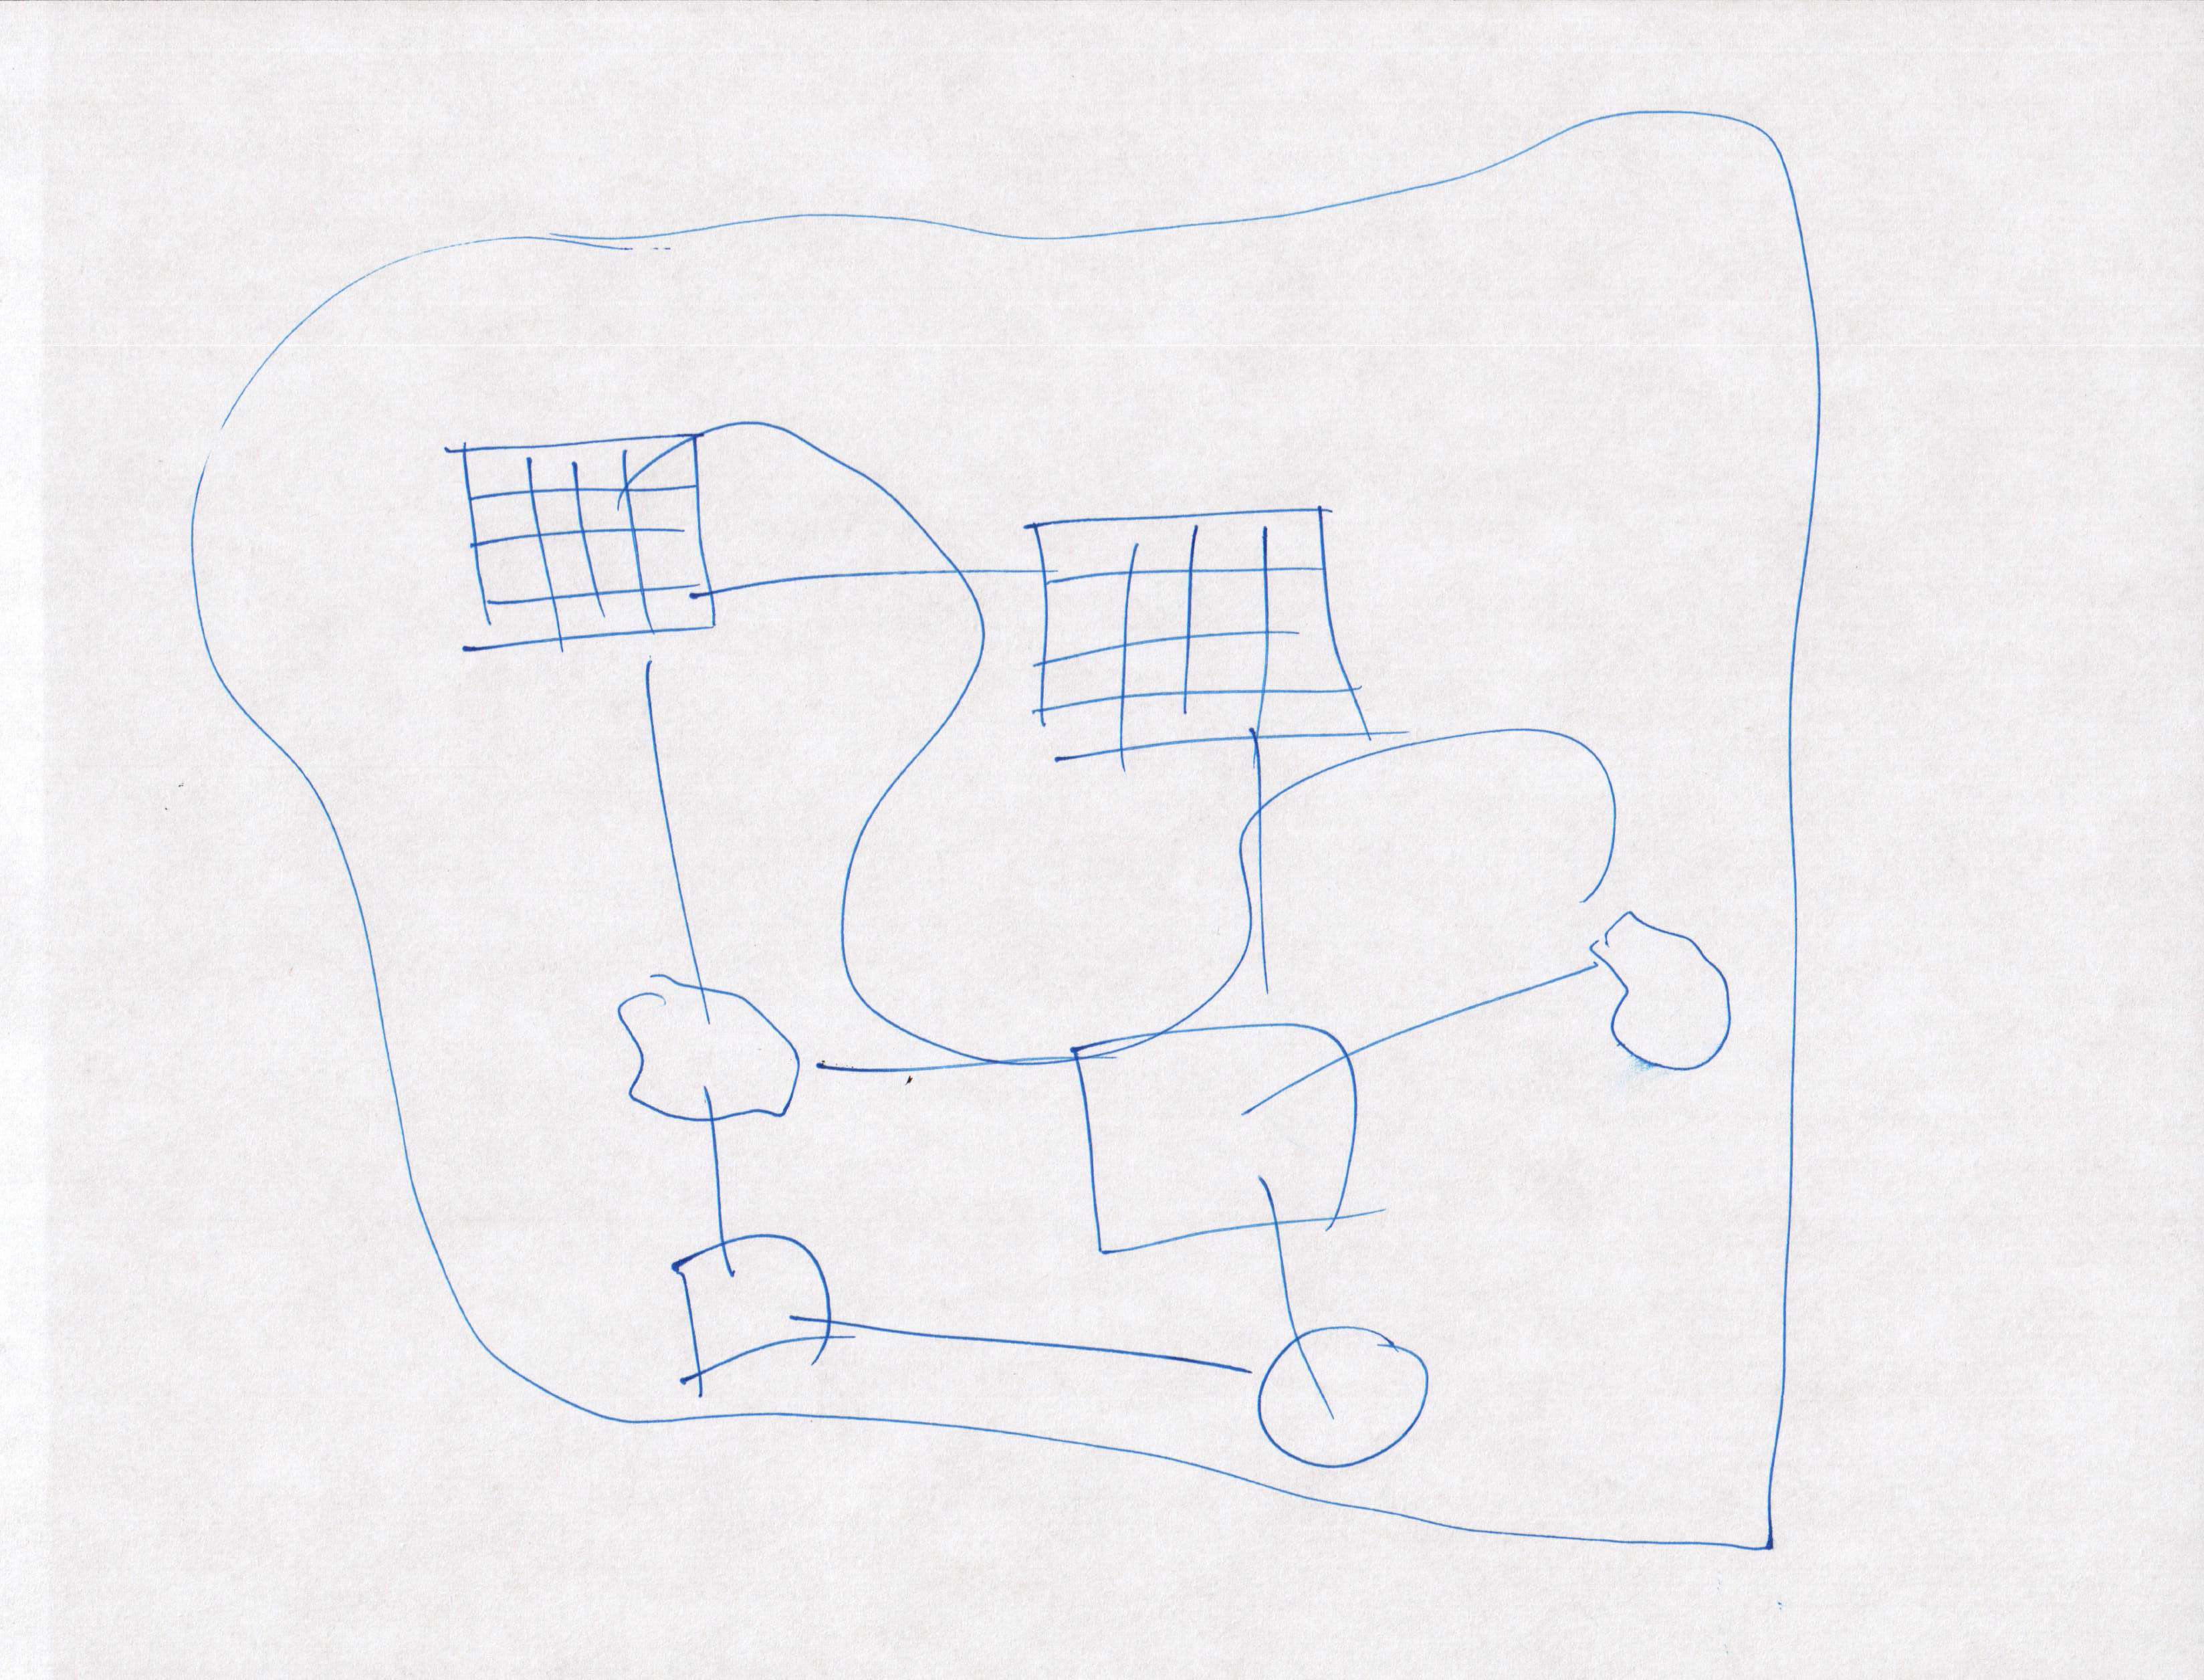
\includegraphics[width=3.45in]{team_code_ownership_images/CodeOwnership.jpg}
\caption{\quotes{Draw how you feel about the code}}
\label{Programmer1}
\end{figure}

The team wants to feel pride in improving code quality.  It feels good to be improving the code design and readability. If the team starts neglecting these concerns, it can engender a sense of disgust and apathy for the code can spread throughout the team.

\subsection{Product Fit}
\textbf{Definition:} Product fit is developers believing that features of the product will satisfy the user's needs.

\textbf{Purpose:} Engineers want to create products that matter to the users. Delivering a product that matters to someone satisfies the self-identity motivation of psychological ownership.

\textbf{Threat: Ignoring user feedback.} When the product manager ignores feedback from user research and usability testing, developers may lose faith in the product's ability to achieve its goals. Developer motivation and engagement can decrease when developers perceive they are building a feature that users have explicitly said they do not want yet is built to solve a business goal. 

\textbf{Threat: Ignoring developers feedback about the product.} Pivotal's balanced team approach is founded on collaboration between product managers, interaction designers, and developers. When product managers or other stakeholders ignore feedback from developers, developers can begin to feel less ownership in the product, and in turn, be less motivated to work on the project. 

%When picking up a story, a developer verifies that the story contains clear acceptance criteria. In the absence of acceptance criteria, the developer typically clarifies what needs to be done with the product manager. On one project during which the stakeholders ignored feedback from the developers, one developer recalled, \participantQuote{In this case, I don't feel like spending the extra energy to go and say, `Hey, are you sure? Is this what you want?'} 

Feature apathy or product apathy can result in a poorly crafted product that does not meet the customer's needs.

\subsection{Team Cohesion}
\textbf{Definition:} Team cohesion is the degree to which team members identify as part of the team, stick together through adversity and take pride in the team's accomplishments \cite{Bollen1990Perceived, Beal2003Cohesion, Whitworth2007Motivation}.

\textbf{Purpose:} Team cohesion satisfies the \quotes{having a place} motivation of psychological ownership.

\textbf{Threat: Distancing a developer from the team.} Team apathy manifests when developers do not feel that they are a part of the team. Developers feel less ownership of the code base when they feel excluded from the team.

We observed several behaviors that can distance a developer from the team: interrupting the developer during discussions, using poor listening skills so that the developer feels unheard, or talking beyond the developer's level of technical expertise. 

On one team, during discussions, the team talked about code but never looked at the source code. One developer found these abstract discussions difficult to follow. Sometimes the team discussed parts of the code that the individual had not seen recently. When the team discussed two variants of coding practices without showing concrete examples, the programmer could not contribute. When the developer raised this issue to the team and the team continued with the status quo, the programmer felt marginalized by the team.

Poor onboarding of developers can contribute to feelings of isolation. On one project, there was a time crunch and the team was feeling the pressure to deliver stories. When the team added developers, the team had a \quotes{sink or swim} attitude, letting new team members figure things out on their own, hence making them feel unwelcome.

When developers feel that the team does not care about them, their sense of ownership can decrease.

\section{Discussion}
\label{Discussion}
\subsection{Transitioning to team code ownership}
\label{Transitioning}

The above results have numerous implications for teams attempting to transition to team code ownership. 

Some developers effortlessly make the transition to team code ownership. They immediately see the benefits of being able to modify any part of the code base and quickly shift from \quotes{I made this} (personal ownership) to \quotes{we made this} (collective ownership.)

Others may struggle with team code ownership for several reasons:

\begin{itemize}  

\item Developers may struggle to transition to a caretaker mindset.  In one interview, a software engineer struggled to describe the developer's relationship with the code on a very challenging project and settled in on the caretaker metaphor: \participantQuote{Sometimes I kind of feel like a janitor to [the code base].  Maybe caretaker would be better. Yeah, probably caretaker. I feel like a janitor just cleans up messes, but a caretaker makes things better.} 

\item A developer may be distraught at \participantQuote{seeing my work slowly removed from the app.} 

\item Developers can no longer take pride in functionality that they exclusively develop.

\item Existing knowledge silos, which hinder team code ownership, may be slow to break down.
 
\end{itemize}

New hires struggling with the transition slowly realize that \participantQuote{Someone else is going to take over and they're going to do fine. I can move onto something else and that's okay.} They recognize the lack of long-term individual authorship, learn to expect their code to be transitory, develop trust in their teammates and thus loosely hold personal contributions. \participantQuote{The code that I write today may be in the code base for a little while, and it will evolve into something better.} Eventually,  they experience the benefits of a collaborative environment: \participantQuote{People are a lot more flexible all across the board, with changing things or accepting feedback or collaborating,} and the team can say \quotes{Hey, this is our code!}

Shifting from individual to team code ownership may requires multiple and complementary practices to actively remove knowledge silos. In this case, daily pair rotation helped combat knowledge silos. Moreover, for developers with strong individual ownership tendencies, sharing ownership first with a small group (where trust and communication come easier) may help. One Pivotal engineer uses improvisation and collaboration games to help teams practice letting go of control, trusting the team, and learning to be pleasantly surprised by what emerges. 

\subsection{Results Evaluation}

The factors influencing team code ownership presented in Section \ref{TeamCodeOwnership}, have emerged from the Grounded Theory research study introduced in Section \ref{SustainableSoftwareDevelopmentTheory}. While other factors may influence team code ownership, we focus only on those that were observed during the study. Grounded Theory studies can be evaluated using the following criteria \cite{Charmaz}: 

\textbf{Credibility:}  The 21 intensive open-ended interviews and numerous field notes from participant-observation serve as a rich and credible data set for the analysis. 

\textbf{Originality:} The paper broadens the idea of team code ownership by acknowledging that collective code ownership is more than a policy statement, and by uniquely identifying factors that affect the team's sense of code ownership.

\textbf{Resonance:} Several participants reviewed our findings and indicated that both the factors and threats resonate with their experience.

\textbf{Usefulness:} The study identifies factors associated with ownership and suggests several ways of engendering team code ownership.

This work analyzed software projects at the Silicon Valley office of Pivotal following Extreme Programming. From an \textbf{external validity} perspective, grounded theory is non-statistical, non-sampling research. Our results therefore cannot be statistically generalized to a population. Rather, researchers and professionals can adapt the concepts and ideas to other contexts case-by-case. 

Finally, our results might be influenced by \textbf{researcher bias} or \textbf{prior knowledge bias}. A risk of the participant-observer technique is that the researcher may lose perspective and become biased by being a member of the team. While a participant-observer gains perspective an outsider cannot, an outside observer might see something a participant observer will miss. Similarly, while prior knowledge helps the researcher interpret events and select lines of inquiry, prior knowledge may also blind the researcher to alternative explanations \cite{GlaserIssues}. We mitigated these risks by recording interviews and having the second and third authors review the coding process. 

\section{Conclusion}
\label{Conclusion}
This paper reports results from a participant-observation, constructivist grounded theory study at Pivotal, a large American software company employing Extreme Programming practices. It provides three main contributions.

1) Our observations clearly indicate that \textbf{team code ownership is a feeling to be engendered not a policy to be decreed}.

2) Meanwhile, both discussions with and observations of participants suggest five factors associated with strong feelings team code ownership. Pivotal developers more acutely feel team code ownership when i) they understand the system context; ii) they have contributed to the code in question; iii) they perceive code quality as high; iv) they believe the product will satisfy user needs; and v) they perceive team cohesion as high.   

3) Moreover, diverse events and trends can undermine sense of ownership, including:  increasing knowledge silos, increasing code base size, increasing team size, inability to contribute, pressure to deliver and deprioritizing continuous refactoring, ignoring user feedback, ignoring developer feedback, and distancing a developer from the team. 

In conclusion, Pivotal's developers find team code ownership highly advantageous; however, transitioning to a team code ownership model is easier for some than others. Some agile practices including continuous pair programming, overlapping pair rotation, continuous refactoring, and test driven development appear to help. Promising angles for future research include more nuanced explorations of the code ownership spectrum, further exploration of the roles of emotion and identity, as well as developing specific practices for facilitating ownership transitions. 

% \section{Acknowledgement}
Thank you to Rob Mee, David Goudreau, Ryan Richard, and Zach Larson for making this research possible.

% \chapter{Constructing Products: Sustainable Software Development}
\label{SustainableSoftwareDevelopmentChapter}

\section{Summary}

\textit{Context:} Conventional wisdom says that team disruptions (like team churn) should be avoided. However, we have observed software development projects that succeed despite high disruption. 
\textit{Objective:} The purpose was to understand how to develop software effectively, even in the face of team disruption.
\textit{Method:} We followed Constructivist Grounded Theory. We conducted participant-observation of several projects at Pivotal (a software development company), and interviewed 21 software engineers, interaction designers, and product managers. The researchers iteratively sampled and analyzed the collected data until achieving theoretical saturation.
\textit{Results:} This research introduces a descriptive theory of Sustainable Software Development. The theory encompasses principles, policies, and practices aiming at removing knowledge silos and improving code quality (including discoverability and readability), hence leading to development sustainability. 
\textit{Limitations:} While the results are highly relevant to the observed projects at Pivotal, the outcomes may not be transferable to other software development organizations with different software development cultures.
\textit{Conclusion:} The theory refines and extends our understanding of Extreme Programming by adding new principles, policies, and practices (including Overlapping Pair Rotation) and aligning them with the business goal of sustainability. 

\section{Introduction}
Imagine being a software development manager when one of your top engineers, Dakota, gives notice and is moving on to a new job opportunity. You are simultaneously excited because the new position provides a great career opportunity for someone you respect, yet distressed that her departure may exacerbate your own project. How will the team overcome this disruption? Your investment in this engineer and her entire accumulated knowledge about the project is evaporating. Dakota developed some of the systems' trickiest, most important components. How long will it take the other programmers to assimilate Dakota's code?  How will this affect their productivity and future development?


Conventional wisdom says that team churn is detrimental to project success and that extensive documentation is needed to mitigate this effect. Unfortunately, documentation quickly becomes out-of-date and unreliable \cite{Lethbridge2003Documentation}, undermining this approach. During a Grounded Theory study, we observed projects succeed despite high disruption and little documentation. This raised the following research question: \quotes{How do the observed teams develop software effectively while overcoming team disruption?}

Exploring this question resulted in a descriptive theory of \quotes{Sustainable Software Development.} The theory explains how a collection of synergistic principles, policies, and practices help develop software effectively while overcoming team disruption. This is done by engendering a positive attitude towards team disruption, encouraging knowledge sharing and continuity, as well as prioritizing high code quality. Here, \textit{team disruption} refers to substantial ongoing changes in team composition, including team members joining or leaving, as well as temporary vacations or leave of absence. 

In Section \ref{RelatedWork}, we present related work on Extreme Programming and team disruption. In Section \ref{ResearchMethod}, we review how we employed Constructivist Grounded Theory to derive a descriptive theory supported by empirical data. We also present the research context, introducing both the company and one of the five projects under study. In Section \ref{Theory}, we describe the theory and how its principles, policies, and practices work together to achieve software development sustainability. In Section \ref{TheoryEvaluation}, we evaluate the theory using established criteria for evaluating a Grounded Theory. In the last sections, we examine threats to research validity, consider future research, and conclude the research.
\section{Related Work}
\label{RelatedWork}
In Extreme Programming \cite{BeckExtremeProgramming2004}, Kent Beck describes a set of interdependent practices that manage feature development (much like Scrum \cite{SchwaberScrum}), as well as technical practices that facilitate a collaborative team environment. Extreme Programming comprises 13 primary practices and 11 corollary practices. 

One Extreme Programming practice, collective ownership, simply means that \quotes{anyone on the team can improve any part of the system at any time.} Beck contrasts collective ownership with \quotes{no ownership} and \quotes{individual ownership.} With collective ownership, every developer takes responsibility for the whole of the system. When developers see opportunities to improve the code, they go ahead and improve it if it makes their life easier \cite{BeckExtremeProgramming2000}. Later, \quotes{collective ownership} was renamed to \quotes{shared code} \cite{BeckExtremeProgramming2004}. 

One Extreme Programming practice contributing to collective code ownership is pair programming. Pair programming is where production code is created by two developers working together at a single computer \cite{BeckExtremeProgramming2004}. Extreme Programming does not prescribe how pairs are formed or for how long a pair works together. Williams presents a pair rotation strategy for maintaining specialization, by \quotes{choosing the right partner for the right situation}  \cite{Williams2002}. People are assigned modules of the code to own based upon expertise and find partners from neighboring modules. While knowledge is shared with pairing, one person owns every story that touches their part of the system, building individual code ownership. In one case study, the project started with a pair rotation strategy based on skillsets but evolved into a daily rotation determined randomly \cite{Vanhanen2007}. Some teams use a pair programing matrix \cite{AlaverdyanPairProgrammingMatrix} (also called a pairing ladder \cite{Davies2009AgileCoaching}) to track who has paired with whom for the purpose of pairing people who have not paired recently.

Truck Number is \quotes{The size of the smallest set of people in a project such that, if all of them got hit by a truck, the project would be in trouble.} \cite{WikiTruckNumber}. Truck Number, or Bus Count, reminds management about the effects of disruptive events for a team. In 1994, Coplien \cite{Coplien1994} mentions \quotes{Truck Number} as a risk to his Solo Virtuoso pattern of using only one talented developer to create a software system. Awati suggests that Truck Number can be increased by reducing complexity, cross-training, and documentation \cite{AwatiBusFactor}, all of which are found in Extreme Programming. However, Extreme Programming implements \quotes{documentation} as discoverable, intention revealing code. Ricca \cite{Ricca2011TruckFactor} examines the difficulty in computing the Truck Number. 

Rigby quantifies turnover using knowledge at risk analysis on abandoned files  \cite{Rigby2016Turnover}. A line of code is abandoned if the most recent contributor has left the company.  A file is abandoned if more than 90\% of the lines in the file are abandoned.  Izquierdo examines how teams managed orphaned code \cite{Izquierdo2009Turnover}. Joseph examines job turnovers to understand the reasons developers leave their company  \cite{Joseph2007Turnover}.  
\section{Research Method}
\label{ResearchMethod}
\subsection{Constructivist Grounded Theory}

We adopted Grounded Theory \cite{Charmaz}, which provides an iterative approach to data collection, data coding, and analysis resulting in an emergent theory. We selected Charmaz' Constructivist approach to Grounded Theory, which \quotes{emphasizes understanding and acknowledges that data, interpretations, and resulting theory depend on the researcher's view} \cite{StolGroundedTheory}. The two primary data sources were field notes collected during continuous participant observations of a seven-month project and interviews with Pivotal software engineers, interaction designers, and product managers. Interviews were recorded, transcribed, coded, and analyzed using constant comparison. In addition, the first author was involved in four other projects as participant-observer.

Grounded Theory immerses the researcher within the context of the research subject from the point of view of the participants. As the research progresses, Grounded Theory allows the researcher to \quotes{incrementally direct the data collection and theoretical ideas.} The theory provides a starting place for inquiry, not a specific goal known at the beginning of the research. As we interact with the data, the data influence how we progress and alter the research direction. When starting a Grounded Theory research study, the core question is, \quotes{What is happening here?} \cite{GlaserTheoreticalSensitivity}. Our initial core question was \quotes{What is happening at Pivotal when it comes to software development?}
\subsection{Participants}
The first author interviewed 21 interaction designers, product managers, and software engineers who had experience with Pivotal's software development process. They were distributed across four different Pivotal offices. Interaction designers identify user needs predominately through user interviews; create and validate user experience with mockups; determine the visual design of a product; and support engineering during implementation. Product managers are responsible for identifying and prioritizing features, converting features into stories, prioritizing stories in a backlog, and communicating the stories to the engineers. Software engineers implement the solution. Participants were not paid for their time. 
\subsection{Data Collection}
We relied on \quotes{intensive interviews,} which are \quotes{open-ended yet directed, shaped yet emergent, and paced yet unrestricted} \cite{Charmaz}. Open-ended questions were used to enter into the participant's personal perspective within the context of the research question. The interviewer attempts to abandon assumptions to better understand and explore the interviewee's perspective. Charmaz \cite{Charmaz} contrasts intensive interviews from informational interviews, which facilitate collecting accurate `facts' and investigative interviews that attempt to reveal hidden intentions or expose practices and policies. 
 
The initial interviews were open-ended explorations starting with the question, \quotes{Please draw on this sheet of paper your view of Pivotal's software development process.} The interviewer specifically did not force initial topics and merely followed the path of the interviewee. 

While exploring new emergent core categories, whenever possible, subsequent interviews were initiated with open-ended questions.  For example, asking the participant, \quotes{Please draw your feelings about the code} often resulted in conversations about code ownership. 

Each interview was transcribed into a Word document with timecode stamps for each segment.

In addition to collecting data from interviews, the first author collected field notes while working as an engineer on the project described in Section \ref{ProjectQuattuor}. The field notes comprised multiple paragraph entries recorded several times a week, collected over seven months. These notes described individual and collective actions, captured what participants defined as interesting or problematic, and included anecdotes and observations. 
\subsection{Data Analysis}
Data analysis began with line-by-line coding as recommended by Charmaz \cite{Charmaz}. Coding line-by-line helps the researcher identify nuanced interactions in the data and avoid jumping to conclusions. The data then advanced from these initial codes to focused codes, focused codes to core categories, and core categories to an emergent theory. 

We reviewed the initial codes while reading the transcripts and listening to the audio recordings. We discussed the coding during weekly research collaboration meetings. To avoid missing insights from these discussions \cite{GlaserTheoreticalSensitivity}, we recorded and transcribed them into grounded theory memos. 

As data was collected and coded, we recorded initial codes in a spreadsheet and we used constant comparison to generate focused codes. Only ideas expressed by multiple interviewees informed focused codes and subsequent analysis. 

We constantly compared new codes to existing codes to refine codes and eventually generate categories. We periodically audited each category for cohesion by comparing its codes. When this became complex, the codes were printed on index cards, and then arranged and re-arranged until cohesive categories emerged. We wrote memos to capture the analysis of codes, examinations of theoretical plausibility, and insights. 

Constant comparison allowed us to identify \quotes{the conceptual relationship between categories and their properties as they emerged} \cite{GlaserBasics}, leading to a resulting descriptive theory. The resulting theory is presented in Section \ref{Theory} and illustrated in Table \ref{SustainableSoftwareDevelopmentTable}. The table includes the main categories and their organization into principles, policies, and practices. Examples of quotes leading to some categories are presented in Table \ref{ChainOfEvidenceTable}.

\begin{table}[t]
\renewcommand{\arraystretch}{1.5}
\centering
\caption{Quotes for Selected Categories}
\label{ChainOfEvidenceTable}
\begin{tabular}{|p{\twoColumnWidth}|}
\hline
Engendering Positive Attitudes Toward Team Disruption \\
\hline
\participantQuote{I'm excited when a new person joins the team. That person has experience that might add something to the project.} \\

\participantQuote{I like that people bring new energy. Projects often get into the state of a lull with the same people working on it and have the same cadence. New people bring a new perspective. [Two engineers recently joined] and it was really cool to see their fresh perspective. I always like people joining a project.} \\

\participantQuote{Team members go out of their way to make new teammates feel welcome and help ramp them up.} \\

\hline
Team Code Ownership \\
\hline
\participantQuote{I feel ownership of the code as a whole, and I feel empowered and able to go and work on any part of the codebase.} \\
\participantQuote{I don't feel like I have [individual] ownership. It's really a collaborative effort to achieve where we are today \ldots I feel like everybody owns this product.} \\
\participantQuote{There is a lot of emphasis that you are not your code.} \\
\participantQuote{I never feel like a specific piece is mine or something belongs to other people.}\\

\hline
Overlapping Pair Rotation \\
\hline
\participantQuote{To make sure that knowledge silos don't form we rotate pairs. As people work on specific stories and specific parts of the code, we want to share that knowledge.} \\

\participantQuote{Rotating pairs reduces knowledge silos and reduces the bus factor. We do not want the departure of one developer from the project to cripple the project.} \\

\participantQuote{We rotate pairs because everyone has a different set of knowledge. When you work with someone you get a little bit of that knowledge. The more you pair with them, the more knowledge you get.} \\

\hline
\end{tabular}
\end{table}


\subsection{Research Context}
\label{ResearchContext}

Pivotal is a large American software company (with 16 offices around the world), which provides solutions for cloud-based computing, big data, and agile development. 

This study focuses on one Pivotal subsidiary, Pivotal Labs, which provides agile developers, product managers, and interaction designers to other firms. Its mission is to deliver highly-crafted software products and provide a transformative experience for clients' engineering cultures. To change the client's development process, Pivotal combines the client's software engineers with Pivotal's engineers at a Pivotal office where they can experience Extreme Programming in an environment conducive to agile development. For startups, Pivotal engineers might be the first to work on the project. For enterprise clients, Pivotal provides additional engineering resources to accomplish new business goals. 

Pair programing ability is a strong pre-requisite for becoming a Pivotal Labs developer. During job interviews, applicants engage in multiple pair-programming rounds to reveal their ability to listen to and empathize with pairs. 

Typical teams include six developers, one interaction designer, and a product manager. The largest project in the history of the Palo Alto office had 28 developers while the smallest had two. Larger projects are organized into smaller coordinating teams with one product manager per team and one or two interaction designers per team. 

Commonly utilized technologies include Angular, Android, backbone, iOS, Java, Rails, React, and Spring. These are often deployed onto Pivotal's Cloud Foundry. 

Pivotal Labs has followed Extreme Programming \cite{BeckExtremeProgramming2004} since the late 1990's. While each team autonomously decides what is best for each project, the company culture strongly suggests following all of the core practices of Extreme Programming, including pair programming, test-driven development, weekly retrospectives, daily stand-ups, a prioritized backlog, and team code ownership.

We only observed teams at Pivotal Labs. Other teams, especially teams in other divisions, might have a different culture and follow different software practices.
\subsection{Project Context: Project Quattuor}
\label{ProjectQuattuor}
While we observed five projects in total, this discussion focuses on Project Quattuor. This project shares many similarities with the other four. To preserve client confidentiality, we can only reveal that Project Quattuor's purpose was to develop a mobile application for controlling expensive equipment.

The project lasted 43 weeks. The initial four weeks, called Discovery and Framing, include four main activities: 1) interaction designers investigate user needs through user interviews, 2) product managers define the features for the initial release based on those needs, 3) interaction designers create an initial interaction design and validate their mock-ups with users, and 4) engineers mitigate technology risks. Discovery and Framing was followed by code implementation, resulting in two releases to both the Apple store and Google Play store.

\begin{figure}[t]
\centering
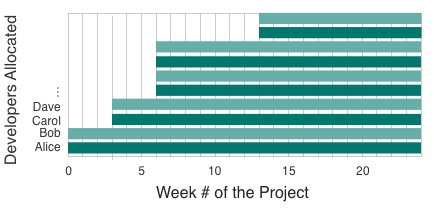
\includegraphics[width=\twoColumnWidth{}]{sustainable_software_development_images/OriginalDeveloperStaffingV3.jpg}
\caption{Planned Developer Staffing}
\label{PlannedDeveloperStaffing}
\end{figure}

The 35-person project consisted of an iOS team of ten engineers, an android team of ten engineers, and a Java back-end team of eight engineers with the support of two to four interaction designers and three product managers. Here we focus on the iOS team. The first iOS release to the Apple store occurred in week 23. Given the success of the project, the client extended the engagement for a second iOS release that happened on week 43. 

Figure \ref{PlannedDeveloperStaffing} shows the staffing plan at the start of Project Quattuor. The plan was to start the project with two developers, while adding more developers as more tracks of work became available. Figure \ref{DeveloperStaffing} shows the actual staffing, which is quite different from the plan.

The bar chart on the top of Figure \ref{DeveloperStaffing} shows when individual developers started and stopped working on the project. Five developers were on the project for most of its duration, while 22 people worked on the project in total. The maximum team size was 12 developers working together at the same time. The graph on the bottom of Figure \ref{DeveloperStaffing} shows the total number of developers allocated to the project at any given week. Developers ramped up from week 5 to week 12, with an average team size of 10 and a maximum of 12 developers.

Developers were routinely rotated and were replaced for various reasons, including promotions, medical leave, leaving the company, transferring to a different office, and vacations. Atypically, the client was more concerned with feature development than cost, so absent developers were replaced, leading to 22 different people working on the same ten-person project. 

The ongoing rotation of team members likely undermined the team's sense of identity \cite{TuckmanModel}. In addition, the project experienced many challenges, including not having access to production back-end systems or expensive dependent physical components, and cultural differences between Pivotal and the client's deployment organization. Yet the team successfully completed the project. The client was delighted, even claiming that the team delivered a multi-year project in five months by delivering the first release. 

Contrary to conventional wisdom, high team disruption did not appear to negatively influence the success of Project Quattuor. This observation raises our research question: \quotes{How do the observed teams develop software effectively while overcoming team disruption?}


%\begin{figure*}[t]
%\centering
%\includegraphics[width=\twoColumnWidth{}]{DeveloperStaffingV4.jpg}
%\caption{Actual Developer Staffing}
%\label{DeveloperStaffing}
%\end{figure*}

\begin{figure}[t]
\centering
\includegraphics[width=\twoColumnWidth{}]{sustainable_software_development_images/DeveloperStaffingV4.jpg}
\caption{Actual Developer Staffing}
\label{DeveloperStaffing}
\end{figure}

\begin{table*}[t]
\renewcommand{\arraystretch}{1.5}
\centering
\caption{Theory of Sustainable Software Development: Principles, Policies, and Practices}
\label{SustainableSoftwareDevelopmentTable}
\begin{tabular}{|p{2.5in}|p{3.5in}|}
\hline
\multicolumn{2}{|c|}{Sustainable Software Development}              
\\
\hline
Underlying Principles & Keeping a Positive Attitude Toward Team Disruption \newline Encouraging Knowledge Sharing and Continuity \newline Caring about Code Quality \\ 
\hline
Policies & Team Code Ownership \newline Shared Schedule \newline Avoid Technical Debt  \\
\hline
Removing Knowledge Silos Practices & Continuous Pair Programming \newline Overlapping Pair Rotation \newline  Knowledge Pollination  \\
\hline
Caretaking the Code Practices & TDD / BDD \newline Continuous Refactoring  \newline Supported by Live on Master \\
\hline
\end{tabular}
\end{table*}


\section{Theory of Sustainable Software Development}
\label{Theory}

Sustainable software development refers to the ability and propensity of a software development team to mitigate the negative effects of major disruptions, especially team churn, on its productivity and effectiveness. Our theory of Sustainable Software Development, summarized in Table \ref{SustainableSoftwareDevelopmentTable}, is targeted towards software developers and has emerged from the Grounded Theory research described above. We hypothesize that sustainability emerges from synergistic principles, policies, and practices, which collectively explain how the observed Pivotal teams overcome disruption. The ability of any pair to work on any story while caring about the code is the primary mechanism by which these principles, policies, and practices mitigate disruption. 

In this section, we document each principle, policy, and practice.  For each policy and practice, we present how it is used at Pivotal, and discuss anti-patterns and potential alternatives. We provide deeper descriptions for practices rarely documented in the literature.
\subsection{Principles}

\subsubsection{Engendering Positive Attitudes Toward Disruption}
Conventional wisdom says that team disruption should be avoided. Yet, team disruption is a reality in the industry, as exemplified by Project Quattuor where only five of 22 developers worked on the project for most of its duration (see Figure \ref{DeveloperStaffing}). However, the observed organization engendered a positive attitude towards disruption, transforming a challenge into an opportunity and hence demonstrating remarkable business agility. Team members rolling off the project were replaced as needed. New members rolling onto the project were viewed as an opportunity to improve the current code base by providing a fresh perspective. When a new team member did not understand the code base, he or she revealed issues with code discoverability. New team members often questioned the team's assumptions and challenged \quotes{cargo culting.} 

The first underlying principle of Sustainable Software Development is engendering an open and positive attitudes towards team disruption, transforming a challenge into an opportunity to improve code quality.

\subsubsection{Encouraging Knowledge Sharing and Continuity}
Despite the fresh perspectives added by new team members, team disruption can precipitate in significant knowledge loss for the organization. Policies and practices that encourage knowledge sharing and continuity mitigate this risk. These policies are Team Code Ownership, and Shared Schedule, while the practices are Continuous Pair Programming, Overlapping Pair Rotation, and Knowledge Pollination (which are discussed below).

The second underlying principle of Sustainable Software Development is encouraging knowledge sharing and continuity, enabling the knowledge to spread from one developer to the next, and eventually reach the entire team. Knowledge sharing and continuity make the team more resistant to disruption. 

\subsubsection{Caring about Code Quality}

Enabling knowledge sharing and continuity does not guarantee sustainable development if the team starts incurring technical debt \cite{McConnellTechnicalDebt}. A set of policy and practices aimed at taking good care of the code itself mitigates this risk. The policy is Avoid Technical Debt, while the practices are Test-Driven Development / Behavior-Driven Development and Continuous Refactoring (which are discussed below).

The third underlying principle of Sustainable Software Development is caring about code quality, hence avoiding technical debt and enabling sustainable team productivity.
\subsection{Policies}

\subsubsection{Team Code Ownership}

\textbf{Description:} Team code ownership is the extent to which any team member can modify any part of the team's code. Code ownership is influenced not only by official policy but also each developer's familiarity with and emotional relationship to the code.

\textbf{Purpose:} Everyone on the team is responsible for the team's code. Simply saying \quotes{Any team member can modify any piece of the code} is not sufficient to achieve the desired result of team code ownership. We documented five factors that affect the team's sense of code ownership and eight risks observed on Pivotal teams \cite{SedanoTeamCodeOwnership}. Achieving team code ownership requires a set of enabling practices. These enabling practices aim at removing knowledge silos and taking good care of the code, as described in the following sections.

\textbf{At Pivotal:} Every developer is empowered to work on any part of the team's code and is encouraged to refactor any code section to improve its quality as needed, especially in cases of low code discoverability and readability.

\textbf{Anti-pattern:} Removing team code ownership makes sustainable software development challenging. Every line of code written via strong ownership might create a knowledge silo. Code reviews are a mitigation strategy with an asynchronous delay. When the delay is too long, merging code onto the master becomes problematic, which discourages Continuous Refactoring. 

\subsubsection{Shared Schedule}
\textbf{Description:} Shared Schedule signifies that all team members have the same work schedule. 

\textbf{Purpose:} Shared Schedule enables Continuous Pair Programming, Overlapping Pair Rotation, and Knowledge Pollination practices. With Shared Schedule, teams form new pairs at the beginning of the day. The evening becomes a natural interruption to the continuous software development workflow. 

\textbf{At Pivotal:} Team members at the Palo Alto office work Monday to Friday from 9:00 am to 6:00 pm. This is done without management coercion; each team member agreed to this fixed schedule to achieve the benefits of Sustainable Software Development. While Shared Schedule is the norm, exceptions are possible. 

Pivotal prefers co-located teams in order to promote synchronous and osmotic communication. Project Quattuor was an exception with the team split between Palo Alto and San Francisco. Each day, developers in one location remotely paired with developers in the other location to spread the knowledge across the two offices.

\textbf{Anti-pattern:} Flexible work hours potentially jeopardizes Continuous Pair Programming, Overlapping Pair Rotation, and Knowledge Pollination practices. A team with flexible work hours might find it difficult to pair program on all stories (as described in the Continuous Pair Programming practice). A team member consistently soloing from 8:00 am to 10:00 am might be building knowledge silos. 

When developers arrive whenever they feel like it, rotating pairs (as described under the Overlapping Pair Rotation practice) becomes awkward, as there is no longer a natural time to rotate pairs. Trying to schedule a time midday to rotate pairs feels artificial. Even if the team says they will rotate later in the day, once pairs get into their stories and form context on what needs to be done, they typically forget about re-pairing until it is time to go home.

Pivotal experimented with pairing when developers arrived, but this meant that developers coming early were making decisions for the team members who arrived later, hence loosing some benefits of pair programming. 

\textbf{Alternatives:} A possible mitigation strategy could be to adopt core work hours. Individuals would solo on simple cleanup chores outside of core hours, and switch to pair programming for feature development when the whole team is in the office. 

\subsubsection{Avoid Technical Debt}
\textbf{Description:} Technical Debt refers to delaying needed technical work, by taking technical shortcuts, usually in pursuit of calendar-driven software schedules \cite{McConnellTechnicalDebt}. 

\textbf{Purpose:} Avoid Technical Debt enables a team to balance feature development with Continuous Refactoring (as described under the Continuous Refactoring practice). When a team is pressured to finish work by a deadline, they might be tempted to focus on feature delivery, take on technical debt, and stop refactoring. When a team delays refactoring and takes on technical debt, the code becomes harder to work with, which in turn makes it more difficult for developers to rotate onto that part of the code base. There is a dialectic tension \cite{RalphProcessTheories} between Continuous Refactoring and delivering more features while accruing technical debt.

\textbf{At Pivotal:} A pair tends to create well-crafted code by avoiding shortcuts and short-term fixes. The team codes for the \quotes{present} by building the simplest solution for the current story. The team eschews over-engineering for potential future features. The team avoids technical debt by building the best solution for the moment at hand. When inheriting a large code base with existing technical debt, we observed a team actively paying down technical debt while delivering new features. 

\textbf{Anti-pattern:} On Project Quattuor, the product manager suggested that the team deliver more stories at the cost of technical debt to make a release date. Some team members followed this suggestion, skipped the refactoring step, and introduced harder to maintain code. This decision made it difficult for pairs to rotate onto parts of the code. Pairs making the decision to skip refactoring caused future pain for the next pair to work with that part of the code. Immediately after the first release, the team spent several weeks refactoring the code to pay down the debt and consistently deliver new features again.
\subsection{Removing Knowledge Silos Practices}
This section presents practices for encouraging knowledge sharing and continuity, enabling the knowledge to spread from one developer to the next, and eventually reach the entire team. This phenomenon is illustrated in Figure \ref{KnowledgeSharing}, where letters A to F represent six developers working in pairs.

\begin{figure}[t]
\centering
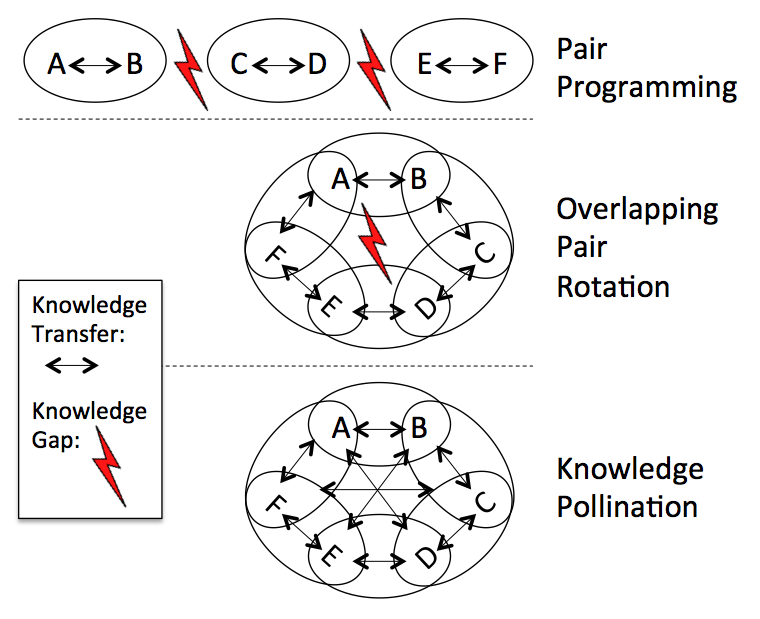
\includegraphics[width=\oneColumnWidth{}]{sustainable_software_development_images/KnowledgeSharingLevels.png}
\caption{Three Levels of Knowledge Sharing}
\label{KnowledgeSharing}
\end{figure}

\subsubsection{Continuous Pair Programming}
\textbf{Description:} Continuous Pair Programming is two developers collaborating to write software together as their normal mode of software development.

\textbf{Purpose:} When two developers work together, they are likely to bring more knowledge, and generate more diverse solutions compared to a solo developer. Additionally, there are many documented benefits of pair programming \cite {Williams2002}. When two developers work together, knowledge spreads from one developer to the next \cite{Zieris2016KnowledgeTransfer}, as illustrated in Figure 3. Overall, pairing reduces knowledge silos and can improve code quality.

\textbf{At Pivotal:} Pairing happens with two monitors, two keyboards, two mice, and one computer. Developers always work in pairs, unless exceptional circumstances arise. For instance, solo programming occurs when one developer is out of the office for part of the day (e.g. at the doctor's office), out of the office the whole day (e.g. out sick), or involved in another business activity for a few hours (e.g. interviewing candidates, scoping a new project). When solo programming, developers take low-risk chores, refactorings, or stories. With any sizable project, there usually is something the team has been meaning to do that one person can safely do and report back to the team on its completion. 

\textbf{Anti-pattern:} Removing this practice results in solo programming where there is a clear owner for the code written. This would increase individual ownership and start creating knowledge silos. 

\textbf{Alternatives:} In solo programming, to remove silos, developers could take the stories for the part of the code they know least about. Assigning stories to developers who have the least understanding of the code could be a hard sell to management as it reduces productivity (at least initially). Bird \cite{BirdDontTouchMyCode} suggests that this approach would introduce more defects. 

\subsubsection{Overlapping Pair Rotation}
\textbf{Description:} Overlapping Pair Rotation happens when there is a rotation of the people working on a track of work: one developer rolls off the track and another developer rolls on, keeping continuity of one developer at each rotation. This results in knowledge continuity for a track of work, as illustrated in Figure 3. Typically, rotations happen in the morning as the evenings provide a natural interruption to the work. 

\textbf{Purpose:} The rotation of developers helps spread knowledge and promotes team code ownership. The goal is to prevent the situation where one or two developers understands how  part of the system works and must be assigned any story related to that part of the system. The entire team should be able to modify the code. Rotation helps prevent knowledge silos and individual code ownership from forming. 

\textbf{At Pivotal:} Whenever a knowledge silo begins to emerge, the team actively fights against it and tries to spread that knowledge around through pair rotation. During the study, three strategies were observed.

\textit{Optimizing for people rotation:} Most teams rotate based on who has paired with whom. Developers try to pair with the person they \quotes{least recently paired with} (basically a Least Recently Used strategy). Some teams use rotation techniques or tools to track this information.

This strategy does not clearly articulate the purpose of knowledge silo removal and the need for knowledge transfer. As an example, developers who recently left a track of work might ask to be rotated back without realizing the potential cost to the team. This prevents an opportunity to spread the knowledge to the rest of the team. (This issue is more serious on larger teams; on a four person team, this is not an issue).

\textit{Optimizing for personal preferences:} A few teams allow developers to pick with whom they will work or on which stories to work based on individual preferences. This has the same downsides as the previous strategy. 

\textit{Optimizing for context sharing:} A few teams are experimenting with rotating onto a track the person who has not been working on the track for the longest time. The goal each day is for the developer leaving the track next to empower the developer who will remain on the track. Before any rotation, the remaining developer is asked, \quotes{Was enough context shared with you?} If the answer is no, then the first developer does not leave and the pair continues to work together for another day. This provides a feedback loop on how well the team is transferring knowledge. 

\textbf{Anti-pattern:} Removing this practice means that developers can work on the same part of the code base for extended periods of time, developing individual code ownership and knowledge silos. One participant described their experience at a previous company that follows Extreme Programming. Developers could be paired for more than a month working on only one part of the system. This lack of pair rotation led to deep knowledge silos. 

Ideally, developers work on the next, non-blocked story at the top of the backlog. When developers start skipping down the backlog, it can be an indication that they might not have enough context to work on any story. On Project Quattuor, a knowledge silo emerged around a complicated bug related to an obsolete technology that only a handful of people understood. Often developers would skip over stories and bugs related to that technology. At one point, the product manager reminded the team to keep \quotes{working from the top of backlog.}

Sometimes a developer wants to see a story through to completion over multiple days. Maybe he or she enjoys the technology or the feature. In these situations, agreeing to the request may result in forming knowledge silos and creating a sense of personal ownership. Statements like \quotes{We need Marion on that story, only she really knows the Apple watch code base,} or \quotes{Shea knows the ins-and-outs of the legacy integration, we need him to work on this story,} suggest that knowledge silos have emerged. 

\textbf{Alternatives:} Team members that build a knowledge silo can share what they learned through a demo, code walk through, or a team huddle. This helps a team share knowledge, but is less effective than working directly with the code. 

\subsubsection{Knowledge Pollination}
\textbf{Description:} Knowledge Pollination refers to the set of activities contributing to knowledge sharing in an unstructured way. Examples include daily stand-up meetings, weekly retrospections, writing or sketching on whiteboards, overhearing a conversation, using the backlog to communicate current status about a story, calling out an update to the entire team, or simply reaching out to others to ask questions as needed. 

\textbf{Purpose:} Knowledge Pollination contributes to spreading knowledge among the team as illustrated in Figure 3.

\textbf{At Pivotal:} Daily standups create awareness of who is working on what. Teams can write down a \quotes{parking lot} of issues to discuss during daily standups. A pair may record the current status of a blocked story so that the next pair picking it up knows the situation. Osmotic communication helps when a developer overhears another pair discussing an issue and offers needed knowledge. Instead of thrashing, a pair interrupts another pair to gain the needed information. Thus, interruptions are encouraged because they make the entire team more efficient as knowledge pollinates across the team. 

Calling out an update to the entire team might be a simple as shouting \quotes{The build is broken, we are looking into it}, or this interchange: \quotes{We just checked in a presenter,} followed by \quotes{We just used your presenter. That's great collaboration.}

While working on a story, a pair may discover that they are missing some key context that prevents them from efficiently proceeding. If the issue is about the acceptance criteria for a story, they clarify with the product manager. If the issue is about the code base, the pair can ask the people who recently worked on that section of code, or ask the entire team. To determine whom to ask, the pair may remember who did what at stand-up, look through Pivotal Tracker (an agile project management tool) to see who worked on a story, or check out source code version history (e.g. git annotate). Two-, four-, and six- person teams seem to have collective memory of who worked on which features from daily standup. 

These mechanisms help a team build awareness. Chong observed that \quotes{transmission of awareness information is a relatively effortless act in the XP environment} in her ethnographic study comparing an Extreme Programming team to a traditional team \cite{ChongNominum}.
 
\textbf{Anti-pattern:} An organization that provides little opportunity to share knowledge leads to wasted time as developers must acquire the knowledge through other means or end up reinventing the wheel.
\subsection{Caretaking the Code Practices}
\subsubsection{Test-Driven Development, Behavior-Driven Development}
\textbf{Description:} In Test-Driven Development (TDD) developers write unit tests before creating a design and writing code. In Behavior-Driven Development (BDD) developers implement acceptance tests before creating a design and writing code. Most lines of production code are tested before the production code is written. The software's design emerges from the tests and subsequent refactorings.

In Extreme Programming, Kent Beck describes his corresponding \quotes{Testing} practice as developers writing \quotes{automated unit tests} and implementing customer provided \quotes{functional tests} for story acceptance \cite{BeckExtremeProgramming2000}. Later, he refines these ideas as \quotes{Test-first programming} \cite{BeckExtremeProgramming2004}. 

\textbf{Purpose:} This practice creates a safety net and empowers a pair to have the confidence to modify the code base. This enables any pair to pick up any story. Continuous Refactoring results in easier to modify tests.

\textbf{At Pivotal:} Developers use a combination of TDD and BDD. While each project is different, programmers tend to use BDD to describe interactions between the user and the system and TDD at a unit test level. Teams use a variety of TDD strategies including testing the responsibilities and interactions \cite{Goose} or contract testing using mocks \cite{RainsbergerIntegrationTestsYouTube}. In Pivotal's ideal, the design emerges from the creation and exploration of the test cases. 

\textbf{Anti-pattern:} Without this testing practice, developers no longer have the confidence to change any part of the code as they may unknowingly end-up breaking something else. 

\textbf{Alternatives:} For a system without a test suite documenting the system specification, a possible remedy is for developers to own particular parts of the system in order to understand the ramifications of changes. Creating strong code ownership and knowledge silos is exactly the problem that sustainable software development is trying to solve.

Writing tests after the code is written could produce a safety net for refactoring, provided that tests correctly exercise the system. (A test that never failed might not be testing anything). We did not observe this behavior and future research is necessary to determine if any testing approach is sufficient for sustainable software development.

\subsubsection{Continuous Refactoring}
\textbf{Description:} Continuous Refactoring is the systematic improvement of the code base concurrently with new feature development. When developers identify something wrong such as a code smell, they simply fix it. In this regard, developers are caretaking the code by continuously improving it. This practice results in an emergent software design, as well as empathy for the code as developers learn to \quotes{listen to the code.} 

%Continuous Refactoring is one way to prevent technical debt from accumulating. When a team employs continuous refactoring, the team refines a code base towards simple design, intention revealing code, and discoverable code. 

\textbf{Purpose:} Continuous Refactoring enables any pair to work on any part of the system. Long-term benefits for the team include increased code discoverability, code readability, code modifiability, and code simplicity. 

\textbf{At Pivotal:} Developers typically do some refactoring while implementing stories. Developers are encouraged to improve the code's design, make the code easier to understand, and increase the discoverability of a component based on its responsibility. Usually, the team prefers \quotes{pre-factoring} where the developer does the complicated work to make the implementation of the current story as simple and easy as possible, as opposed to \quotes{post-factoring} where refactoring happens after the story is done, but before it is delivered. 

\textbf{Anti-pattern:} Removing this practice might produce difficult to modify and messy code. Developers might not be able to easily work on any part of the code base. When refactoring is skipped, code might be simply bolted on to the existing design. Soon it becomes increasingly difficult to bolt more code on. A dilemma arises for the programmers working on the next story: do they continue bolting on more code, or do they perform the pretermitted refactorings? Removing this practice may also result in hard-to-change tests.

\textbf{Alternatives:} Postponing refactoring may be necessary in extreme situations, for instance, when the company might go out of business unless the company releases the next version. In such situations, the team risks taking on uncontrolled technical debt as \quotes{refactoring later} turns into \quotes{refactoring never.} 

\subsubsection{Live on Master}
\textbf{Description:} Live on master means that developers integrate their code several times a day, as quickly as possible. ExtremeProgramming.org calls this practice \quotes{Integrate Often} \cite{WellsIntegrateOften}.

\textbf{Purpose:} For teams to continuously refactor and minimize the waste of merge conflicts, the entire team needs to routinely merge their code onto master. If a pair communicates to the team that they are actively \quotes{refactoring} a component, they are asserting exclusive temporary ownership over the file to avoid merge conflicts. While this is a normal practice for a few hours, if it happens for multiple days, the team is losing collective ownership of that code. The team is not able to receive any of the benefits until the work is merged back to master. 

\textbf{At Pivotal:} In the ideal workflow, developers merge their code to master many times a day. If a pair has not merged to master by the afternoon, the pair typically starts examining why this is difficult and explores ways of incrementally making changes. Developers may use branches to save spikes. When rotating pairs, developers may use branches to move work-in-progress code between machines. 

\textbf{Anti-pattern:} Removing this practice means that code lives in branches for days or weeks. Integrations might be painful due to merge conflicts and developers might delay needed refactorings. If a developer has code only on their machine, then no one else on the team can use or modify that code. When code lives only on one machine for many days in a row, the machine acts as a \quotes{virtual branch.} Running a Continuous Integration box and having long running branches is an anti-pattern.
\section{Theory Evaluation}
\label{TheoryEvaluation}

Charmaz identifies four criteria for evaluating a Grounded Theory: credibility (\quotes{Is there sufficient data to merit claims?}), originality (\quotes{Do the categories offer new insights?}), resonance (\quotes{Does the theory make sense to participants?}), and usefulness (\quotes{Does the theory offer useful interpretations?}) \cite{StolGroundedTheory}. 

\textbf{Credibility:} The current data set is rich and its analysis leads to theory saturation. (Saturation means that the properties of the theory are complete and are not affected by new data.) The data set comprises 21 intensive interviews conducted in four different offices, field notes from participant observation on Project Quattuor, and the first author's involvement in four other projects as participant-observer.

\textbf{Originality:} The theory uniquely depicts the principles, policies, and practices enabling software development sustainability in an organization. Since the organization under study follows Extreme Programming, it is not surprising that many of the practices of Sustainable Software Development are defined in Extreme Programming. However, overlapping pair rotation and its supporting principles, policies, and practices are central and unique to the proposed theory.

\textbf{Resonance:} The participants examined the theory. The theory resonates with their experience and reflects the way they work.

\textbf{Usefulness:} The theory informs Pivotal engineers as to why Pivotal purposefully avoids knowledge silos, and how the theory's principles, policies, and practices work together to accomplish the team's goals. The theory explains why the principles, policies, and practices should be incorporated together. A few managers use  the theory to help potential clients understand how Pivotal achieves the business goals of both the client and Pivotal.

\section{Threats to Validity}

\subsection{External Validity}

\textbf{Generalizability across situations:} Grounded Theory does not support statistical generalization from a sample to a population. The results may not be applicable to other teams or other domains. There are four broad types of scientific generalization: 1) from data to descriptions, 2) from descriptions to concepts, 3) from concepts to theory, 4) from theory to description \cite{Lee2003generalizing}. Grounded Theory research involves the first three kinds of generalization. Generalizing from a theory tested in one context to descriptions of a new context (the fourth kind of generalization) could be done by the researchers in the new context, on a case-by-case basis. However, we have not attempted to perform any type four generalizations at this time.

\subsection{Internal Validity}
\textbf{Researcher bias:} A risk of the participant-observer technique is that the researcher may lose perspective and become biased by being a member of the team. An outside observer might see something the researcher missed. We mitigated this risk by recording interviews and with a colleague reviewing the coding process.

\textbf{Prior knowledge bias:} With Grounded Theory, prior knowledge can aid the researcher in looking at interesting research questions or create difficulties by blinding the researcher about possible explanations \cite{GlaserIssues}. We mitigated this risk with a colleague reviewing the coding process. 
\section{Future Research}
We are interested in the tension between individual and team ownership, as well as the factors that foster and decrease the sense of ownership. Developers, interaction designers, and product managers all have different goals for their role. In future work, we plan to examine how the sense of ownership is driven by different factors for each role.

Some programmers naturally adapt to team code ownership, while others struggle with the transition. Future research could follow new Pivotal engineers and examine their journey in transitioning from individual code ownership to team code ownership. Perhaps there are 
specific practices that Pivotal or the development team could employ to ease the transition. We could also investigate the optimal team size for team code ownership, or explore whether Sustained Software Development works for a distributed team with a Shared Schedule.
\section{Conclusions}
This research introduces a descriptive theory of \quotes{Sustainable Software Development} as a solution to the challenge of software development sustainability for an ever changing workforce. The theory emerged from a Constructivist Grounded Theory research study. By collecting data from 21 intensive interviews conducted in four different Pivotal offices, field notes from participant-observation on the Project Quattuor, and the first author's involvement in four other Pivotal projects as participant-observer, the study investigates the research question \quotes{How do the observed teams develop software effectively while overcoming team disruption?}

The emergent theory is characterized by a collection of synergistic principles, policies, and practices encouraging a positive attitude towards team disruption, knowledge sharing and continuity, as well as caring about code quality. The theory refines and extends Extreme Programming by adding principles, policies, and practices (including Overlapping Pair Rotation) and aligning them with the business goal of sustainability.

Conventional wisdom says that team disruptions should be avoided, and that extensive documentation is needed to prevent knowledge loss during team churn. Unfortunately, documentation often quickly becomes out-of-date and unreliable. The theory positions team code ownership with overlapping pair rotation and knowledge pollination as an alternative and potentially more effective strategy to mitigate against knowledge loss.

The primary benefits to the software developer are the ability to understand the entire system, the ability to work on every story, increased in teaching opportunities to share one's expertise, and more nuanced understanding of the utilized technologies. 

The primary benefit to the employer is business agility. The engineering team continues to deliver software week after week, month after month, while surviving cataclysmic events. Things do not fall apart when the superstar developer leaves because features or components are not critically tied to a particular individual. Critical feature work can be parallelized since anyone can work on any feature.  The whole team's talents are leveraged.

% \section{Acknowledgement}

% Thank you to Rob Mee, David Goudreau, Ryan Richard, and Zach Larson for making this research possible. Thank you to Karina Sils for creating Figure \ref{PlannedDeveloperStaffing} and Figure \ref{DeveloperStaffing} using Sketch.



% \chapter{Removing Waste}
\section{Summary}

\textit{Context:} Software development is a complex socio-technical activity that involves coordinating different disciplines and skill sets and thus provides ample opportunity for waste to emerge. Waste is any activity that produces no value for the user.
\textit{Objective:} The purpose is to understand observed wastes in software development.
\textit{Method:} Following Constructivist Grounded Theory, we conducted a two-year participant-observation of several software development projects at Pivotal, interviewed 26 software engineers, interaction designers, and product managers, and analyzed one year of retrospection topics. We iterated between analysis and theoretical sampling until achieving theoretical saturation.
\textit{Results:}  This chapter introduces the first evidence-based waste taxonomy, identifying eight wastes along with causes and tensions within wastes. It also provides a comparison with the taxonomy of wastes found in Lean Software Development.
\textit{Limitations:} While the results are highly relevant to Pivotal, the outcomes might not apply to organizations with different software development cultures.
\textit{Conclusion:} The waste taxonomy serves as a starting point for waste identification and elimination. Comparing this taxonomy to Lean Software Development's list of wastes revealed our taxonomy's parsimony and expressiveness while illustrating wastes not covered by previous work. 

\section{Introduction}
\participantQuote{The engineers are depressed. The project grinds them down\ldots It is hard to know which problem to tackle first. There is coupling everywhere\ldots Each layer of the system has unnecessary complexity\ldots The depth of knowledge about the system is super thin\ldots There is a lot of waiting\ldots Building the java code takes ten minutes. Starting the server takes seven minutes. Running the javascript tests take two minutes. Running the integration tests take 47 minutes. Continuous integration takes \textit{forever} to run all the tests and get the code onto the acceptance environment. \newline \indent There is waste everywhere. \textemdash Software Engineer on Project Septem}

Software development is a complex socio-technical activity that involves coordinating different disciplines and skill sets. Identifying user needs, crafting features for those needs, identifying and prioritizing value, implementing features, releasing and supporting products provide ample opportunity for waste to creep in. 

Here, \quotes{waste} refers to \quotes{any activity that consumes resources but creates no value} for customers \cite{WomackLeanThinking}. Eliminating waste, by definition, improves efficiency and productivity. 

However, eliminating waste can be difficult not least because \textit{identifying} waste can be difficult.  Numerous cognitive phenomena including status quo bias \cite{JostDecadeOfSystemJustification} hinder practitioners' propensity and ability to notice waste in existing practices. Identifying the types of waste that often occur in software projects  may, therefore, facilitate our ability to identify and eliminate waste. Identifying and eliminating waste is a key principle of lean manufacturing. 

The Toyota Production System \cite{OhnoToyotaProductionSystem, ShingoToyotaProductionSystem} transformed manufacturing from batch-and-queue to just-in-time. The similarities between batch-and-queue and waterfall, as well as just-in-time and iterative software development, inspired several software development methods \cite{PoppendieckLeanSoftwareDevelopment, AndersonKanban}. These methods adapt, in a top-down fashion, lean principles for software environments. 

However, manufacturing differs from software development in significant ways. Software is intangible and practically free to duplicate. Two customers can buy the same software in a way they cannot buy the same car. A software developer can produce a wider variety of products than an assembly line. While most factories build batches of near-identical goods, much software remains unique. The cost structure is fundamentally different since the variable costs of software are near zero, while cars have high variable cost and higher fixed costs for factories. 

Given the obvious differences between developing software and manufacturing physical products, software development may entail waste types never envisioned by the literature on lean manufacturing. Even the most careful adaptation of lean principles for software may not have identified such waste types. Therefore, we report an in-depth, longitudinal investigations of a successful software company to address the following research question: 

\textbf{Research Question: \quotes{What are observed wastes in software development?}}

Any software development process does instill repeated activities such as taking a story off a backlog or writing test cases which can be optimized. One goal would be to make these processes efficient and repeatable in a similar context. 

We briefly review the history of lean in Section \ref{HistoryOfLean} and review related work in Section \ref{RelatedWork}. Section \ref{ResearchMethod} describes our research method. We present the emergent waste taxonomy in Section \ref{SEWaste}. We then compare this model with the waste list from Lean Software Development in Section \ref{LeanSoftwareDevelopmentComarison}. We then evaluate the results, present limitations, and conclude in Sections \ref{ResultsEvaluation} and \ref{Conclusion}.

\section{A Brief History of Lean}
\label{HistoryOfLean}

The Toyota Production System prioritizes waste removal by creating a culture that pursues waste identification and elimination in the entire production of a vehicle \cite{OhnoToyotaProductionSystem, ShingoToyotaProductionSystem}. In 1945, Toyota optimized for the production rate of each system, keeping like machines near each other. Ohno rearranged equipment so that the output of one machine fed into the next machine, slowed machines down to have the same cadence, and only produced material when it was needed. After optimizing Toyota's factories, Toyota then trained their suppliers so that the entire production of a vehicle was just-in-time, transforming from mass production to lean production. The resulting \quotes{pull} system was easy to reconfigure, minimized inventory, and supported short production runs.  

Based on analysis of the Toyota Production System, Lean Thinking \cite{WomackLeanThinking} describes a process of identifying and removing waste using five principles:
\begin{enumerate}
\item Specify value: define value from the customer's perspective
\item Identify the value stream: examine all actions required to bring raw materials to final product for the customer and eliminate any obvious unnecessary steps
\item Flow: re-engineer from batch-and-queue to just-in-time or continuous flow 
\item Pull: create products only in response to a customer order
\item Perfection: continue with a continuous process of waste identification and elimination
\end{enumerate}

Analyzing the value stream involves identifying three types of activities: activities that clearly create value; activities that create no value for the customer but currently necessary to manufacture the product; and activities that create no value for the customer, are unnecessary and therefore should be removed immediately, i.e., waste.

The Toyota Production System characterized seven types of manufacturing waste \cite{ShingoToyotaProductionSystem} shown in Table \ref{ManufacturingWaste}. Later, Womack and Liker each added a waste type \cite{WomackLeanThinking, LikerToyotaWay}.

\begin{table}[t]
\renewcommand{\arraystretch}{1.5}
\centering
\caption{Toyota Production System Definition of Manufacturing Waste}
\label{ManufacturingWaste}
\begin{tabular}{|p{2in}|p{4in}|}
% \begin{tabular}{|p{0.85in}|p{2.3in}|}
\hline

Waste Type                & Description                                                                                                                                                  \\ \hline
Inventory                 & The cost of storing materials until they are needed. Sometimes the material is never used.                                                                   \\ \hline
Extra Processing          & The cost of processing that is not needed by a downstream step in the manufacturing process. (Sometimes an inefficiency from not seeing the entire process.) \\ \hline
Overproduction            & The cost of producing more quantity of components than necessary for the present.                                                                            \\ \hline
Transportation (of goods) & The cost of unnecessarily moving materials from one place to another place.                                                                                  \\ \hline
Waiting                   & The cost of waiting for a previous upstream step to finish.                                                                                                       \\ \hline
Motion (of people)        & The cost of unnecessary picking up and putting things down.                                                                                                  \\ \hline
Defects                   & The cost of rework from quality defects.                                                                                                                     \\ \hline
Value                     & The cost of producing goods and services that do not meet the needs of the customer.                                                                         \\ \hline
Non-utilized Talent       & The cost of unused employee creativity and talent.                                                                                                           \\ \hline
\end{tabular}
\end{table}

\section{Related Work}
\label{RelatedWork}
We could not find any evidence-based publications on software engineering waste. This section provides one non-empirical waste taxonomy followed by several observational studies that applied Value Stream Mapping to software development.

Mary and Tom Poppendieck contributed the most influential body of work in the area of software waste. In creating Lean Software Development \cite{PoppendieckLeanSoftwareDevelopment}, the Poppendiecks adapted Lean Thinking and the Toyota Production System from manufacturing to software development. Their comparison of manufacturing waste with software waste is presented in Table \ref{ManufacturingVersusLeanSoftwareWaste}.
 
\begin{table}[t]
\renewcommand{\arraystretch}{1.5}
\centering
\caption{Comparison of Manufacturing Waste with Lean Software Development Waste}
\label{ManufacturingVersusLeanSoftwareWaste}
\begin{tabular}{|l|l|}
\hline
Toyota Production System's Manufacturing Wastes & Poppendieck's Software Development Wastes \\ \hline
Inventory                                       & Partially Done Work                       \\ \hline
Extra Processing                                & Relearning                                \\ \hline
Overproduction                                  & Extra Features                            \\ \hline
Transportation (of goods)                       & Handoffs                                  \\ \hline
Waiting                                         & Delays                                    \\ \hline
Motion (of people)                              & Task Switching                            \\ \hline
Defects                                         & Defects                                   \\ \hline
Value (added by Womack in 1996)                 & N/A                                       \\ \hline
Non-utilized Talent (added by Liker in 2004)     & N/A                                       \\ \hline
\end{tabular}
\end{table}

The Poppendieck's mapping is top-down in the sense that they ask, what is the equivalent of each type of manufacturing waste in a software context. However, some types of manufacturing waste (e.g., transportation and motion) which rely on physical attributes may not map well to software development which is intangible while software development may exhibit new types of waste not present in manufacturing. This motivates a complementary bottom-up empirical research in software development contexts to identify and characterize different types of waste. 

The Poppendiecks suggest \quotes{the five biggest causes of policy-driven waste:} complexity, economy of scale, separating decision making from work, wishful thinking, and technical debt \cite{PoppendieckResultsNotPoint}.

Power and Conboy leverage the Poppendieck's model by combining it with literature in manufacturing, lean production, product development, construction, and healthcare. They shift from using wastes of inefficiencies to impediments to flow. \cite{PowerImpediments}

Petersen and Wohlin examined the flow of features by creating cumulative flow diagrams through the different development phases at Ericsson AB in Sweden and India. (The phases are detailing features, implementing and unit testing features, isolation testing, system testing, and ready for release.) They defined several metrics to identify bottlenecks, variance in hand-overs, and cost types. For cost savings analysis, they define waste as any feature that has work done on it (e.g. \quotes{describing the feature}) but is never released to a customer \cite{Petersen2011}.

Several studies applied Value Stream Mapping to software development. Value Stream Mapping popularized by Womack systematically examines each stage for waste. Interestingly, these studies only found the waste of waiting rising from a batch-and-queue system \cite{Ali2016, Khurum2014, Mujtaba2010}. One study identified the wastes of motion and extra processing from interviews, not the current state map \cite{Mujtaba2010}.

Khurum said, \quotes{the researchers found it is more suitable to start focusing on improvement potential based on long waiting or lead time.} During the waste identification step of the workshop with their research participants, they ask attendees \quotes{in which phase do we see the majority of waiting?} \cite{Khurum2014} The Pygmalion effect (self-fulfilling prophecy) may explain why the researchers only found \textit{waiting} waste in Value Stream Mapping analysis.

Ali et al applied information flow modeling to Value Stream Mapping which revealed \textit{waiting} waste from the passing of big batches from group to group and missing prioritization \cite{Ali2016}.

These studies typically reduced waste by switching the organization from waterfall to iterative software development or reducing the batch size in iterative software development \cite{Ali2016, Khurum2014, Mujtaba2010}.
\section{Research Method}
\label{ResearchMethod}
\subsection{Constructivist Grounded Theory}
We used Constructivist Grounded Theory \cite{Charmaz}, which involves iteratively collecting and analyzing data to generate and refine an emergent theory. Grounded Theory research begins by asking, \quotes{What is happening here?} \cite{GlaserTheoreticalSensitivity}; or in this case, \quotes{What is happening at Pivotal when it comes to software development?} \textit{Removing Waste}  later emerged as a core category.
\subsection{Research Context: Pivotal Labs}
Pivotal Labs is a division of Pivotal\textemdash a large American software company (with 17 offices around the world). Pivotal Labs provides teams of agile developers, product managers, and interaction designers to other firms. Its mission is not only to deliver highly-crafted software products but also to help transform clients' engineering cultures. To change the client's development process, Pivotal combines the client's software engineers with Pivotal's engineers at a Pivotal office where they can experience Extreme Programming \cite{BeckExtremeProgramming2004} in an environment conducive to agile development. 

Typical teams include six developers, one interaction designer, and a product manager. The largest project in the history of the Palo Alto office had 28 developers while the smallest had two. Larger projects are organized into smaller coordinating teams with one product manager per team and one or two interaction designers per team.

Interaction designers identify user needs predominately through user interviews; create and validate user experience with mockups; determine the visual design of a product; and support engineering during implementation. Product managers are responsible for identifying and prioritizing features, converting features into stories, prioritizing stories in a backlog, and communicating the stories to the engineers. Software engineers implement the solution. 

Pivotal Labs has followed Extreme Programming \cite{BeckExtremeProgramming2004} since the late 1990's. While each team autonomously decides what is best for each project, the company culture strongly suggests following all of the core practices of Extreme Programming, including pair programming, test-driven development, weekly retrospectives, daily stand-ups, a prioritized backlog, and team code ownership. We only observed teams at Pivotal Labs. Other teams, especially teams in other divisions, might have a different culture and follow different software practices.
\subsection{Data Collection}
This discussion analyses data from three sources: 1) interviews with Pivotal employees, 2) topics discussed in 91 retrospection meetings, and 3) participant observation of seven projects over two years. To preserve client confidentiality, we can only reveal limited information about each project:

\begin{itemize}
\item Project Unum (two product managers, four developers) was a greenfield project providing a web front end for installation, configuring, and using a multi-node cluster with big data tools. 
\item Project Duo (two interaction designers, two product managers, six developers) added features to a print-on-demand e-commerce platform. 
\item Project Tes (one interaction designer, one product manager, six developers) added features to management software for internet service providers.
\item Project Quattuor (two interaction designers, three product managers, 28 developers) developed two mobile applications and a backend system for controlling expensive equipment.
\item Project Kvin (one interaction designer, one product manager, six developers) was a greenfield project for a healthcare startup. 
\item Project Ses (two interaction designers, one product manager, ten developers) was adding features and removing technical debt to an existing internet e-commerce website.
\item Project Septem (two interaction designers, three product managers, twelve developers) was adding features and removing technical debt to an existing virtual machine management software.
\end{itemize}
\subsubsection{Participant Observation}
The first author collected field notes while working as an engineer on all seven projects. These notes describe individual and collective actions, capture what participants found interesting or problematic, and include anecdotes and observations.
\subsubsection{Interviews}
The first author interviewed 26 interaction designers, product managers, and software engineers who had experience with Pivotal's software development process from five different Pivotal offices. Participants were not paid for their time.

We relied on \quotes{intensive interviews,} which are \quotes{open-ended yet directed, shaped yet emergent, and paced yet unrestricted} \cite{Charmaz}. Open-ended questions were used to enter into the participant's personal perspective within the context of the research question. The interviewer attempts to abandon assumptions to better understand and explore the interviewee's perspective. Charmaz \cite{Charmaz} contrasts intensive interviews with informational interviews (collecting facts), and investigative interviews (exposing hidden intentions, practices or policies).

The initial interviews were open-ended explorations starting with the question, \quotes{Please draw on this sheet of paper your view of Pivotal's software development process.} The interviewer specifically did not force initial topics and merely followed the path of the interviewee. While exploring new emergent core categories, whenever possible, we initiated subsequent interviews with open-ended questions. The first author transcribed each interview with timecode stamps for each segment. These interviews were spread across the duration of the research study. 
\subsubsection{Retrospection Topics}
When \textit{removing waste} emerged as a core category from interviews and participant observation, we began collecting data from retrospection meetings. A retrospection meeting (or retro) is a meeting to pause, reflect, and discuss the work done during the week, i.e., a safe place where any team member can discuss any issue \cite{DerbyAgileRetrospectives}. Retros are typically scheduled every Friday afternoon. The entire team and important stakeholders attend these meetings. 

The observed Pivotal teams mostly use an emotion-based retro format where \quotes{happy,} \quotes{meh,} and \quotes{sad} faces are written on the top of a whiteboard. The happy-face column represents items that are working well, of which the team wants to do more. The meh-face column represents  items that the team needs to \quotes{keep an eye on.} The sad-face column represents items that are not working well, which the team should try to fix. Any team member can add any topic to any column. After a few minutes, the team dot-votes on the topics to discuss \cite{DerbyAgileRetrospectives}. The team uses the remainder of the sixty-minute meeting to discuss topics. Sometimes discussing a topic is sufficient to affect change, other times the team creates action items. 

We collected data from 91 retrospection meetings over 59 weeks from Projects Quattuor, Kvin, and Ses. (There are more meeting than weeks since each of Project Quattuor's three teams held its own retro each week.)

For co-located teams, the first author took a picture of the whiteboard at the end of the retro and later transcribed the topics into a master spreadsheet. For distributed teams, we copied data from the on-line spreadsheets the team used in place of a whiteboard. Attendees often wrote a short phrase as a proxy for a larger idea. For example, \quotes{Scope} represents \quotes{Too much scope is causing the team stress} or \quotes{Legal} represents \quotes{Waiting on Legal to approve the legal process.} When the provided topic was too vague, we solicited a more detailed description from an engineer present in the meeting. This produced 663 total items for analysis. 
\subsection{Data Analysis}
We began by iteratively collecting and analyzing interview transcripts and participant observations. We used line-by-line coding \cite{Charmaz} to identify nuanced interactions in the data and avoid jumping to conclusions. We reviewed the initial codes while reading the transcripts and listening to the audio recordings. We discussed the coding during weekly research collaboration meetings. To avoid missing insights from these discussions \cite{GlaserTheoreticalSensitivity}, we recorded and transcribed them into grounded theory memos. As data was collected and coded, we stored initial codes in a spreadsheet and we used constant comparison to generate focused codes.

We routinely compared new codes to existing codes to refine codes and eventually generate categories. We periodically audited each category for cohesion by comparing its codes. When this became complex, we printed codes on index cards, and then arranged and re-arranged until cohesive categories emerged. We wrote memos to capture the analysis of codes, examinations of theoretical plausibility, and insights.

When \textit{removing waste} appeared as a core category, we began collecting and analyzing data from retrospectives to investigate (theoretical sampling). After removing irrelevant topics (e.g. complaints about the weather), we printed each retro item onto an index card with its original retro topic, enhanced description, id, and team name (see Figure \ref{exampleRetroTopicl}).

Over the course of two days, two researchers with first-hand experience of the projects did initial coding of the retro topics and merged duplicate topics. We rearranged initial coding categories to be near similarly themed categories and iteratively combined and reorganized categories (see Table \ref{ChainOfEvidence} for example classification). We often stopped to record new insights. When the categories began to stabilize, we compared each category against the other categories looking for relationships. Once we felt that the categories were stable, we performed a final review of each category to verify that the cards belonged to it. 

We continued theoretical sampling for removing waste in additional interviews and participant observations until no further waste-related categories were evident, i.e. theoretical saturation. 


\begin{table}[t]
\renewcommand{\arraystretch}{1.5}
\centering
\captionof{figure}{Example Retro Topic Index Card }
\label{exampleRetroTopicl}
\begin{tabular}{|l|}
\hline
Topic: Legal \\ \\ Description: Waiting on Legal to approve legal pages \\ \\ Id: 182 Project: Quattour\\ \hline
\end{tabular}
\end{table}








\begin{table}[ht]
\centering
\captionof{figure}{Examples for Cognitive Hindrance Waste}
\label{ChainOfEvidence}
\begin{tabular}{|llll|}
\hline
\multicolumn{4}{|l|}{}  \\
\multicolumn{4}{|l|}{Waste category: Cognitive hindrance}  \\
    & \multicolumn{3}{l|}{Cause category: Emotional stress}          \\
    &     & \multicolumn{2}{l|}{Cause property: Low team morale} \\
    &     &      & Retro Topic: Frustrated clients / Pivotal developers       \\
    &     &      & Retro Topic: Negative attitudes                \\
    &     &      & Retro Topic: Apathy                            \\
    &     &      & Retro Topic: Unacknowledged by management      \\
    &     &      & Retro Topic: Messy code                        \\
    &     &      & Retro Topic: Pairing fatigue                   \\
    &     &      & Retro Topic: Poor lighting, lack of windows    \\
    &     & \multicolumn{2}{l|}{Cause property: Rush mode} \\
    &     &      & Retro Topic: Fixed features with a fixed timeline \\
    &     &      & Retro Topic: Aggressive timelines \\
    &     &      & Retro Topic: Scope creep \\
    &     &      & Retro Topic: Repeatedly saying \quotes{This has to be done today} \\
    &     &      & Retro Topic: Long days \\
    &     &      & Retro Topic: Overtime \\
    &     & \multicolumn{2}{l|}{Cause property: Lack of empathy} \\
    &     &      & Retro Topic: Not listening \\
    &     &      & Retro Topic: Criticizing in public \\
    &     &      & Retro Topic: Difficult pairings \\
    &     &      & Retro Topic: Interpersonal conflict \\
    &     &      & Retro Topic: Kicking product out of the team space \\
    & \multicolumn{3}{l|}{Cause category: Cognitive load}          \\
    &     & \multicolumn{2}{l|}{\dots} \\
    & \multicolumn{3}{l|}{Cause category: Context Switching}          \\
    &     & \multicolumn{2}{l|}{\dots} \\
\hline
\end{tabular}
\end{table}


\section{Results: Types of Waste in Software Engineering}
\label{SEWaste}

\begin{table}[t]
\renewcommand{\arraystretch}{1.3}
\centering
\caption{Types of Software Development Waste}
\label{Waste}
\begin{tabular}{|p{1.5in}|p{1.6in}|p{2.8in}|}
\hline
Waste                                 & Description                                                                                                         & Observed Causes                                                                                                                                                                                                                                                                                                                                                                                                                     \\ \hline
Building the wrong product or feature & The cost of building a feature or product that does not address user's needs or desiderata.                                  & \textit{User Desiderata:} not doing user research, validation, or testing; ignoring user feedback; working on low user value features \newline \textit{Business Desiderata:} not involving a stakeholder; slow stakeholder feedback                                                                                                                                                                                  \\ \hline
Mismanaging the backlog               & The cost of duplicating work or expediting lower user value features.                                                       & Backlog inversion; duplicated story; forgetting to start a story; starting too many features                                                                                                                                                                                                                                                                                                                                         \\ \hline
Unnecessary complexity  & The cost of creating a more complicated solution than necessary,  a missed opportunity to simplify features, user interface, or code.      & Unnecessary feature complexity; unnecessary technical complexity; big design up-front; duplicating code; lack of design reuse;                                                                                                                                                                                                                                                                                                                 \\ \hline
Rework                                & The cost of altering delivered work that does not meet the expectations of product managers, interaction designers or users.    & Rejected Stories \newline \textit{No clear definition of done:} ambiguous story; second guessing design mocks; \newline \textit{Defects and Bugs:} poor testing strategy; not doing root-cause analysis on bugs; delaying testing or critical bug fixing                                                                                                                                                                    \\ \hline
Unnecessary cognitive effort          &   The cost from the unneeded expenditure of mental energy.                                                                                                                 & Inefficient tools and problematic APIs, libraries, and frameworks  \newline \textit{Sluething information:} unclear bug reports; messy code; unclear commit messages; knowledge loss from team churn \newline\textit{Suffering from technical debt:} hard to change code
                                                                     \\ \hline
Cognitive hindrance           & The cost of decreasing cognitive capacity or ability.                        & \textit{Emotional Stress:} low team morale; rush mode; lack of empathy \newline \textit{Cognitive Load:} complex stories; noisy output from tools; \newline \textit{Context switching:} delayed feedback causing context switching; product manager taking a long time to accept or reject a story; unavailable product manager or interaction designer                                                                                                                                                        \\ \hline
Waiting                               & The cost of idle time, often hidden by multi-tasking. The cost of not having the needed information or resources to get one's work done. & Slow tests or unreliable tests \newline Unreliable acceptance environment \newline Missing information, people, or equipment                                                                                                                                                                                                                                                                            \\ \hline
Ineffective communication             & The cost from incomplete, incorrect, misleading, inefficient, or absent communication.                         & Team size is too large \newline \textit{Asynchronous communication:} distributed teams; non-collocated stakeholder; dependency on another team; opaque processes outside team \newline \textit{Imbalance:} dominating the conversation; not listening \newline \textit{Inefficient meetings:} lack of focus; skipping retros; not discussing blockers each day; meetings running over (e.g. long standups) \\ \hline                  
\end{tabular}
\end{table}

We identified eight types of waste listed in Table \ref{Waste}. In this section, we define, elaborate, and give examples of each type. When observed, we provide tensions with respect to the waste.
\subsection{Waste: Building the wrong feature or product}
Building features (or worse, whole products) that no one needs, wants, or uses obviously wastes the time and efforts of everyone involved. We observed this waste affecting team morale and team code ownership \cite{SedanoTeamCodeOwnership}. Clearly, this can affect customer satisfaction. 

The product features for Project Ses were designed based on a given persona\textemdash i.e. a fictional, archetypal user \cite{Grudin2002personas}. However, consulting several real intended users revealed that the persona was deeply flawed as the users did not need the product, (the intended users invalidated the persona.) Building the intended product would have been risky and probably wasteful. 

\textbf{Tension: User needs} versus \textbf{business wants.}
Some projects exhibit a tension between user needs and business goals. Practitioners may struggle to produce something that simultaneously satisfies the users and the business.

For example, on Project Quattuor, the client wanted to add a news feed to a mobile phone application that controlled a real world product. However, user validation revealed that no users wanted this feature, and several reacted quite negatively. Despite numerous conversations, the marketing department insisted on adding the feature. 
\subsection{Waste: Mismanaging the backlog}
A product backlog can be mismanaged in several ways, leading to delays of key features or lower team productivity. 

For example, we observed engineers on several projects working on low-priority stories through \quotes{backlog inversion.} This occurs when the engineers working through the backlog get ahead of the project manager who is prioritizing the backlog. For instance, the product manager might prioritize the next ten stories in the backlog, but the engineers get to story 15 before the product manager gets back to prioritizing. This creates waste as engineers implement potentially outdated, low-value, or even counterproductive stories ahead of high-value stories.   

Mismanaging the backlog can also lead to duplicated work in at least three ways. For example, we observed duplicated stories in the backlog, two engineers working on the same story because one had forgotten to change its status in the backlog software (Pivotal Tracker), and two engineers independently addressing the same pain point (e.g. making the build faster) by not adding chores to reflect their work in progress.

\textbf{Tension: Writing enough stories} versus \textbf{writing stories that will never be implemented.}
Pivotal product managers attempt to provide the team with a steady stream of ready, high-value work. This creates a tension between writing enough stories for the team to work on and \quotes{over-producing} stories that might never be implemented. Writing too few stories wastes the team's time while writing too many stories wastes the product manager's time. We observed teams running out of work on rare occasions; we did not observe product managers writing too many stories.  

\textbf{Tension: Finishing features} versus \textbf{starting too many features.}
Product managers decompose a feature into a set of stories, and typically sequence the stories to finish just enough of each feature before starting another feature in order to create the minimal viable product as soon as possible. 

On Project Quattuor's backend system, we observed one product manager starting too many tracks of work at once by prioritizing a breadth of features instead of finishing started features. Unfortunately, several tracks of work were not completed by the first release date. The work in progress was disabled with feature flags. Starting work, changing priorities, and halting work in flight, can result in waste.

Pivotal prefers to maintain a shippable product while finishing minimal viable product versions of each feature as soon as possible. 

\subsection{Waste: Unnecessary complexity}
\textit{Unnecessary complexity} can be caused by complex features (which reduces the user's satisfaction), technical complexity, and unnecessary unique interaction designs (both of which reduces the team's productivity.) 

When a product or feature is unnecessarily complex, it wastes users' time, especially when users struggle to understand how to apply it to achieve their objectives. The anfractuous product is difficult to use. Some features bring unnecessary technical complexity as a simpler interaction design would have solved the same problem. %\sout{We observed a simple solution was to increase conversations with product, design, and engineering. On one project, an engineer shortened the feedback loop by daily checking-in with the interaction designer.}

Similarly, an unnecessarily technical complexity wastes developers' time with unduly difficult to build and maintain code. On Projects Tes, Ses, and Septem, complicated legacy components were refactored into simpler, easier to understand components. Sometimes personal goals do not align with the team goals leading to unnecessary complexity. A Pivotal engineer said that a client engineer's attitude was, \participantQuote{the more complicated, the better, as that means my role is the more important.}

Another way to increase system complexity is through unnecessary uniqueness, i.e., building a new component instead of reusing an existing component. In code, unnecessary uniqueness manifests as duplicated code. In mockups, unnecessary uniqueness results in \quotes{design snowflakes} which could take advantage of design reuse. On Project Duo, the interaction designer created a left-to-right navigational flow for configuring the product but designed a top-to-bottom navigational flow for the checkout page. Both sequences allowed the user to change a previous choice, jump to the correct page, and invalidate dependent information. In retrospect, development time would have shortened if both used the same design treatment. On Project Quattuor, the presence of multiple designers resulted in different design treatments for the same concept. The product shipped multiple versions of layouts, lists, alerts, and buttons, some with expensive interactions to engender user delight. On Project Kvin, the interaction designer created two sets of form inputs which necessitated multiple CSS styles for the HTML form input tags. Singular designs require engineering to build unique solutions with no possibility of reuse.   

\textbf{Tension:  Big design up-front} versus \textbf{incremental design.}
Many projects exhibit a tension between up-front and incremental design. Rushing into implementation can produce ineffective emergent designs, leading to expensive rework. However, big up-front design can produce incorrect or out-of-date assumptions and inability to cope with rapidly changing circumstances, also leading to expensive rework. The desire to avoid rework and differing development ideologies, therefore, motivate tension and disagreement over big design up-front versus incremental design. 

The observed teams expected the product features to change even when the client had clearly defined the project. On all projects with interaction designers, after the interaction designer conducted user research and discovered new information about the user's needs, the feature set changed. No amount of up-front consideration appears sufficient to predict user feedback. The Pivotal teams preferred delivering functionality incrementally and delay integrating with technologies until a feature requires it. For example, an engineer would only add asynchronous background jobs technology when working on the first story to require the needed technology, even if the team knew it would need it on day one of the project.

We observed teams using common architectural and design solutions from similar, previous projects without explicit architectural or design phases.
\subsection{Waste: Rework}
In this study, participants distinguish between rework, revising delivered work that was not done correctly, and new work, improving existing work based on new information. For example, improving a feature based on new user feedback is new work, while rewriting a buggy test case is \textit{rework}.  \textit{Rework}, by definition, wastes resources and developer time. 

We observed numerous sources of \textit{rework} including stories with no clear definition of done, rejected stories, defects in the code, poor testing strategy, ambiguous mock-ups, and delaying testing or critical bug fixing.

On Project Ses, the engineers showed a finished story to the interaction designer for feedback. The interaction designer pointed out a missing interaction, yet the desired behavior was not in the story and not described in the mock-up.

On Project Quattuor, the client delayed fixing of critical bugs until just before the release. Fixing one bug in the backend system had a cascading effect with the clients which expected the code to work a certain way. \textit{Rework} could have been avoided had the critical bug been fixed prior to the client code becoming dependent on it.

On Project Quattuor, the interaction designers created mockups optimized for English, not the target language. After implementing the application, the team realized that the primary foreign language translation took up more space than the English translations, requiring rework for several design components. 

On Project Kvin, the interaction designer did not consider a responsive web design for mobile phones when building the mock-ups. After building a few screens, the team realized that the website did not work well on mobile devices requiring \textit{rework}.

\textbf{Tension: Responding to change} versus \textbf{thrashing.}
While the ability to respond to change quickly is a core tenet of agile development; time, effort, and resources can still be wasted by changing features too often (thrashing). Here, we are trying to distinguish between rapidly improving a product based on new information and repeated, capricious tweaking. 

On Project Kvin, for example, the launch was delayed while the business fiddled with the sequence and number of steps in the user registration process. Project Duo was similarly delayed by a project manager repeatedly resequencing an order customization process. 


% \sout{A related tension is initial velocity versus avoiding rework, that is, the where developers commit code knowing it will need rework to make this sprint's deadline. Reworking the code becomes a story for a future sprint. This is a good example of counterproductive incentives and how workplace monitoring leads to performances that reduce productivity. Is this the kind of thing we want to talk about here? If not, maybe we can cut this tension.}

\subsection{Waste: Unnecessary cognitive effort}
When team members or users have \textit{unnecessary cognitive effort}, their energy and time are wasted. \textit{Unnecessary cognitive effort} includes the waste from sleuthing missing information, knowledge loss from team churn, suffering from technical debt, inefficient tools, and problematic APIs.

We observed several instances of engineers sleuthing for needed information when, for example, code and commit messages did not convey intention, or bug reports were incomplete. Similarly, in projects where knowledge silos formed, team churn leads to wasted effort regaining lost knowledge. Context switching creates similar time and effort waste (see \textit{waiting} waste description for more detail). 
 
Technical debt refers to delaying needed technical work, by taking technical shortcuts, usually to meet a deadline \cite{McConnellTechnicalDebt}. We observed teams suffering from technical debt with long-running, existing code bases. On Project Tes, running the test suite produced 87,000 lines of output including deprecation warnings, exceptions, and test noise. Engineers ignored the overwhelming output which contained important information. With considerable effort, the team fixed the test output to only contained test failures. On Project Ses, dead code littered the code base along with convoluted objects. Project Septem suffered from engineers introducing an idea in one part of the code base, but not applying the concept systematically. The project had multiple CSS themes, multiple test suites using different programming languages, multiple naming conventions, and multiple ways of interacting with the data repositories. On each of these projects, the teams spent considerable effort paying down technical debt to improve their productivity and team code ownership \cite{SedanoTeamCodeOwnership}.  

On Project Quattuor, the product managers were busy managing up as well as providing enough stories to keep the teams occupied. As a result, product managers frequently delayed accepting and rejecting stories. Developers might restart a rejected stories they finished awhile ago requiring them to recall the context around the story. The team followed pair rotation from sustainable software development \cite{SedanoSustainableSoftware} which meant that the pair picking up a rejected story was probably not the pair that worked on it.

In several projects, meanwhile, we observed ineffective tooling (development environments, deployment processes) and convoluted, nonfunctional, premature, complicated, unstable, outdated, unsupported, time-consuming, or inappropriate-for-the-task software libraries leading to engineers working ineffectively. One frustrated software engineer said that one arcane technology \participantQuote{makes me angry enough that I want to hack into it, expose how useless and horrible it is and wipe this miserable product off the face of the earth!}
\subsection{Waste: Cognitive hindrance}
\textit{Cognitive hindrance} is anything that decreases the cognitive capacity and cognitive ability, much like a \quotes{debuff} from role playing games. This waste decreases the person's individual productivity. We particularly observed productivity problems related to emotional stress, cognitive load, and context switching.

On Project Quattuor, for example, the team rushed to release a fixed feature set by a fixed date. They even had a countdown to the release date on an office whiteboard. We observed low team morale, rush mode, lack of empathy, and waiting too long to resolve interpersonal issues leading to people working inefficiently. The team furthermore felt that over-emphasizing the deadline was increasing stress and leading to poor technical decisions, and eventually erased the countdown from the whiteboard. Participants felt that fixing both scope and schedule was antithetical to Pivotal's software process, where the client either chooses the release date and gets the features ready by then or chooses key features and ships the product when the features are ready. 
\subsection{Waste: Waiting}
Having developers waiting around, working slowly or working on low-priority features because something is preventing them from proceeding on high-priority features wastes their time. For example, we observed developers waiting on (or looking for) product managers and designers to clarify a story's acceptance criteria. On Project Quattuor, product managers started multitasking while accepting stories because the acceptance environment was unreliable. We saw team members waiting around because of missing video-conferencing equipment. 
Ohno described \textit{waiting} waste as hidden waste since people start working on the next job, instead of waiting \cite{OhnoToyotaProductionSystem}. To expose this waste, in Toyota Production System, when someone pulls the red cable, everyone stops, bringing attention to the waste. On Project Ses, engineers were waiting hours for the build. It took 58 minutes to run locally and 17 minutes on the build machine due to parallelization on four machines. Team members would not run tests locally, but push code as a branch to the build machine. While the build machine ran the tests, the engineers would either wait or context switch onto different work. If the branch passed, some time later, they would merge their code into the team's code. If the branch failed, the engineers would decide to finish the work that they were doing or switch back and fix the issue. Some engineers found the context switching exhausting. The \quotes{sollution} for \textit{waiting} created \textit{cognitive hindrance} waste.

\textbf{Tension: Wait, block or guess.}
When needed information is missing, engineers appear to have three options: 1) wait for the information; 2) suspend (block) the story and work on something else; 3) act without the information. The best option depends on how far into the story the pair is, how long they have to wait, and their confidence in their best guess.

\textbf{Tension: Waiting} versus \textbf{context switching.}
While engineers are waiting, they often work on something else. However, task switching decreases productivity and increases mistakes \cite{MonsellTaskSwitching}. For short waits, it is therefore probably less wasteful for engineers to just take a break like play table tennis than to switch to another work task. 

\subsection{Waste: Ineffective communication}
\textit{Ineffective communication} is the cost from incomplete, incorrect, misleading, inefficient, or absent communication. We observed large team sizes, asynchronous communication, imbalance in communication, and inefficient meeting reducing team productivity.

We observed issues with asynchronous communication on Project Quattuor. The team was distributed between two offices located an hour apart. We observed the team using remote pairing and engineers commuting between the offices to mitigate the effects of a large distributed team. Even still, communication issues were a perennial theme in the retrospections.


On Project Ses, we observed that one person dominated meetings which prevented quieter personalities from sharing their perspective. 

On Project Quattuor, when the project started, the iOS team did not have a retro and was also lacking a way to make decisions. Adding weekly retros enabled the team to reflect and respond to problems. Over several weeks, the remaining teams added their own retro. 

%When teams are not co-located, additional time is spent on asynchronous communication. Instead of dialoguing about an issue, time is spent crafting a message, sending it, waiting for a response, and interpreting the response. When the message is misunderstood, resolving it takes longer than synchronous communication. When the team is distributed, it loses the benefits of osmotic communication.

%Increasing team size increases the number of communication paths. The number of paths is N x (N -1) / 2. 


% On Project Quattuor, \participantQuote{not enough listening in iOS technical meeting} appeared in two retros. 

% \textit{Ineffective communication} is a well studied topic. \cite{LencioniDeathByMeeting, CollaborationExplained, TabakaCollaborationExplained}.

\section{Comparing to Lean Software Development}
\label{LeanSoftwareDevelopmentComarison}

In this section we compare our taxonomy of software engineering waste presented in Section \ref{SEWaste}, with Lean Software Development's taxonomy of waste. Our goal is to not to critique either model, but to see how the software engineering waste model incorporates features of the Lean Software Development model \cite{PoppendieckConceptToCash}. 

\quotes{It is incumbent upon the researcher to compare and show the variations as different properties under different conditions and then integrate them. \ldots The job is to generate, not verify} \cite{GlaserTheoreticalSensitivity}. 


\begin{table}[t]
\renewcommand{\arraystretch}{1.5}
\centering
\caption{Comparison to Lean Software Development Waste}
\label{LeanSoftwareDevelopmentComparison}
% \begin{tabular}{|p{1.57in}|p{1.57in}|}
\begin{tabular}{|l|l|}
\hline
Software Development Wastes           & Poppendiecks' Software Development Wastes \\ \hline
Building the wrong product or feature & Extra features                            \\ \hline
Mismanaging the backlog               & Partially Done Work                            \\ \hline
Unnecessary complexity                & Not described                             \\ \hline
Rework                                & Defects                                   \\ \hline
Unnecessary cognitive effort          & Relearning                             \\ \hline
Cognitive hindrance           & Task switching                             \\ \hline
Waiting                               & Delays                                    \\ \hline
Ineffective communication             & Not described                             \\ \hline
Not observed                          & Handoffs                                  \\ \hline
\end{tabular}
\end{table}
\subsection{Common to both models}
\textbf{Building the wrong feature} and \textbf{Extra features}: In our model, \textit{building the wrong feature} describes building low-value features for the user. Pivotal's process relies on user validation to assess value in solving the user's needs and iterating from a minimal viable product. In Lean Software Development, \textit{extra features} describes adding in features that are not yet necessary for the product. Lean Software Development mentions the cost of managing, implementing, compiling, integrating, testing, and maintaining unneeded code \cite{PoppendieckLeanSoftwareDevelopment}.  Both perspectives align on delaying features until necessary. 

\textbf{Mismanaging the backlog} and \textbf{partially done work}: In our model, \textit{mismanaging the backlog} represents sequencing low priority work before high priority work or accidentally duplicating work. In Lean Software Development, \textit{partially done work} is work that is not tested, implemented, integrated, documented, or deployed. Any feature description that is not implemented, any code that is not integrated or merged, any code that is untested, any code that is not self-documenting or documented, and any code that is not deployed where the user can receive value is \textit{partially done work}.

In observing Pivotal, teams do not view materials flowing through the system as waste. Interaction designers need to be producing just enough mockups, product managers need to be writing just enough stories, the developers need to be writing just enough code to make the story work. In any continuous flow system, there is unfinished materials at each step. 

While we did observe a product manager that started too many features at once (as described in \textit{mismanaging the backlog} waste section), we mostly observed work flowing in a relatively orderly fashion as compared to a waterfall software process. If we were to observe large amount of waiting designs, or large amounts of waiting stories, then we would classify that waste as \textit{mismanaging the backlog}.

There is common ground between both models on reducing large batch sizes into smaller batches with an ideal of  \quotes{continuous flow,} where work is routinely moving through the system. 

\textit{Mismanaging the backlog} describes observed wastes not covered by \textit{partially done work.}

%Just-in-time production is antithetical to large batch sizes. In any continuous flow system, there is unfinished materials at each step. 

%Based on this understanding of continuous flow, we believe that \textit{\partially done work} is suggesting that large batch sizes need reducing.   

%The Toyota Production System creates buffers of parts at certain steps in the pipeline, like a bumper sits waiting to be used on the next car. Once that bumper is consumed, the process of creating another bumper just like it is started. Enough material is produced to keep continuous flow moving. Ohno was concerned about the stockpiles of inventory stored in warehouses.

%Since Pivotal engineers follow Test Driven Development / Behavior Driven Development, strive to get the tested code into the developer's master branch as quickly as possible, and release frequently, we did not observe the waste associated with partially done work. At any moment in time, an interaction designer is creating a future mock, a product manager is updating a future story, a developer is testing code that has not shipped. This describes the continuous flow of features to the customer. 

\textbf{Rework} and \textbf{Defects}: In our model, \textit{rework} includes mistakes made by the product managers (in writing acceptance criteria), the interaction designers (in creating mockups) and the developers (in writing tests and code). Poor testing strategies, and delaying testing can cause rework. In Lean Software Development, \textit{defects} are the coding mistakes of developers. Therefore the two models align on \textbf{defects} and our model broadens the waste definition with \textit{rework}. \textit{Rework} is a superset of \textit{defects}. 

\textbf{Unnecessary cognitive effort} and \textbf{Relearning}: In our model, \textit{unnecessary cognitive effort} includes the waste from sleuthing for missing information, knowledge loss from team churn, and suffering from technical debt. In Lean Software Development, \textit{relearning} is \quotes{rediscovering something we once knew} \cite{PoppendieckConceptToCash}. Included in \textit{relearning} is failing to engage people in the development process. We did observe product managers having difficulty in involving certain stakeholders, which we include in the \textit{building the wrong product or feature} waste. \textit{Relearning} is only one form of \textit{unnecessary cognitive effort}.

\textbf{Cognitive hinderance} and \textbf{Task switching}: In our model, \textit{cognitive hinderance} includes the waste from emotional stress, cognitive load, and context switching. In Lean Software Development, \textit{task switching} is the cost from trying to multitask or work on more than one task at a time. (Based on our analysis, task switching appears to be a cause, not a waste type.) The desire to have developers work on one thing at a time is common to both models. \textit{Cognitive hinderance} is a superset of \textit{task switching}.  

\textbf{Waiting} and \textbf{Delays}: In our model, \textit{waiting} includes delays from not having the needed information or resources to get one's work done as well as the cost of slow tests and unreliable tests. In Lean Software Development, \textit{delays} are \quotes{waiting for people to be available who are working in other areas} to provide needed information that is not available to the developers. \cite{PoppendieckConceptToCash}. Both wastes describe the cost of missing needing information. \textit{Waiting} is a superset of \textit{delays}.
\subsection{Observed only in Lean Software Development}

\textbf{Handoffs}: \textit{Handoff} waste is the loss of tacit knowledge when work is handed off to colleagues.

We did not observe this as Pivotal follows an iterative software development process with cross functional teams. We did observe \textit{waiting} waste as engineers might contact people outside the team who had needed information. If we were to observe handoffs, then we would classify the subsequent waste as \quotes{sleuthing information} as part of \textit{unnecessary cognitive effort.} 
\subsection{Observed only in our model}
The analysis revealed that Lean Software Development waste taxonomy does not handle the following waste types: \textit{Unnecessary complexity}, and \textit{Ineffective communication}. This suggests that the taxonomy needs expanding to cover our observed cases of waste. For more detail about each of the wastes, see Section \ref{SEWaste}.
\section{Results Evaluation}
\label{ResultsEvaluation}
While other factors may affect software engineering waste, we focus only on those that we observed during the study. Grounded Theory studies can be evaluated using the following criteria \cite{Charmaz, StolGroundedTheory}:
\textbf{Credibility}: \quotes{Is there sufficient data to merit claims?}  This study relies on two years of participant-observation, 26 intensive open-ended interviews, and the agenda of one year's worth of retrospections. 
\textbf{Originality}: \quotes{Do the categories offer new insights?}  This is the first study of waste in software development based on empirical evidence. Prior work is anchored in concepts from manufacturing which might force the model with preconceived ideas. 
\textbf{Resonance}: \quotes{Does the theory make sense to participants?} Several participants reviewed our findings and indicated that the waste taxonomy resonates with their experience.
\textbf{Usefulness}: \textbf{Does the theory offer useful interpretations?} This study acknowledges software development wastes that are not identified in manufacturing. This study explains why certain behaviors, events, and actions can cause software engineering waste. This study provides a rich waste taxonomy for Value Stream Mapping in software development. 

This work analyzed software projects at the Silicon Valley office of Pivotal following Extreme Programming. From an \textbf{external validity} perspective, grounded theory is non-statistical, non-sampling research. Our results, therefore, cannot be statistically generalized to a population. Rather, researchers and professionals can adapt the concepts and ideas to other contexts case-by-case.

Finally, our results might be influenced by \textbf{researcher bias} or \textbf{prior knowledge bias}. A risk of the participant-observer technique is that the researcher may lose perspective and become biased by being a member of the team. While a participant-observer gains perspective an outsider cannot, an outside observer might see something a participant observer will miss. Similarly, while prior knowledge helps the researcher interpret events and select lines of inquiry, prior knowledge may also blind the researcher to alternative explanations \cite{GlaserIssues}. We mitigated these risks by recording interviews and having the second and third authors review the coding process and reviewed the detailed retro topics.

Since Pivotal follows iterative software development, we did not observe wastes commonly associated with the waterfall approach. We know that \textit{waiting} waste is present in other organizations that hand feature documents from one team to another team or use large batch sizes of features \cite{Ali2016, Khurum2014, Mujtaba2010}.

Pivotal has relied on Extreme Programming for almost two decades. While Pivotal attempts to remove waste whenever possible, as a \quotes{lean} software development organization, there may be additional wastes not observed in this research study. 
\section{Conclusion}
\label{Conclusion}
We present the first evidence-based taxonomy of software engineering waste, identifying several waste types together with their causes and tensions. Each waste is illustrated with examples taken from observed projects at Pivotal, showing how the waste materializes, and in some cases how it is removed or eliminated. We also compare our proposed taxonomy to the one found in Lean Software Development.

The proposed taxonomy emerged from a Constructivist Grounded Theory research, including the collection and analysis of data coming from two years of participant-observation of seven software development projects, interviews of 26 software engineers, interaction designers, and product managers, as well as one year of retrospection topics. The analysis of the retrospection topics reveals that the observed Pivotal teams care very much about finding and eliminating wastes in their software development process. The retrospection topics are a treasure trove illustrating many different types of waste. 

Contrary to the Lean Software Development's taxonomy of wastes, which is top-down because created by mapping manufacturing wastes to software wastes, our taxonomy is bottom-up as it is grounded in empirical data. The comparison of the two models shows some alignment. However, our taxonomy expands the Lean Software Development's taxonomy by broadening the definition of most wastes and introducing additional wastes not previously identified. As such, our taxonomy is more expressive and more accurately describes our observed data.

Future research includes continuing to validate the resonance of the proposed waste taxonomy with additional participants at Pivotal. This might involve collecting more data and evolving the taxonomy accordingly. Also, we would like to investigate how Pivotal relies on feedback loops as a mechanism for identifying, dealing with, and reducing waste. 

%\sout{At the core of Lean Thinking is waste identification and elimination \cite{WomackLeanThinking} which is a key differentiator between Lean and Agile in software development \cite{Fitzgerald2015continuous}. (Agile does promote the use of feedback loops which we observed as a common solution for waste identification and removal at Pivotal.)

%Ohno and Shingo singularly focused on the efficiency of the production line through continuous waste removal. By excluding product development activities, the design of the vehicle, they overlooked the entire picture. This may explain why their waste taxonomy misses aspects fundamental to product design.

%In applying waste removal to software development, it behooves the software community first to start with a waste taxonomy grounded in data from software development, not borrow from a dissimilar domain. Since waste removal is core to the Lean movement, starting with an ill formulated waste taxonomy suggests a possible fundamental impact on Lean Software Development claims.

%This work suggests that evidence-based research yields insights grounded in data that have not emerged from applying manufacturing concepts to software development.}

%\sout{Based on the research from value stream mapping, the first step of waste reduction may be switching a software firm from a batch-and-pull process where a feature document is handed to a team to implement (e.g. a waterfall system) to a system where a small number of features are handed to a team (e.g. iterative software development.) Then introducing and reducing feedback loops to remove additional waste.}
% \section*{Acknowledgement}
% Thanks to Ben Christel for his assistance in sorting retro topics and helping with the initial analysis. Thank you to Rob Mee, David Goudreau, Ryan Richard, and Zach Larson for making this research possible.




\appendix
\chapter{Appendix Chapter}
\section{Appendix Section}
Test in main

\chapter{Interview Transcriptions}
% \section{2015-05-29 Product Manager Interview}

\textbf{Todd:} Thank you. 00:01

\textbf{Interviewee:} Yes. You're welcome. 00:02

\textbf{Todd:} I was hoping you could describe your typical day. 00:04

\textbf{Interviewee:} My typical day, okay. We start every morning with stand up. It takes about five minutes. And that's where we go over what we did yesterday or what we're going to do today, any blockers or anything like that. I think the format differs from project to project but usually that's how I like to do it. 00:24

\textbf{Interviewee:} Then, I'll go through emails just to have some alone time and just go through my emails and things like that. And if I'm working with a client PM, we will then start going through the backlog. We might pair on writing stories. We might prioritize the backlog. 00:44

\textbf{Interviewee:} Usually, during the beginning of the week, we'll have an iteration planning meeting. It takes an hour and that's where we'll go through and go over some of the stories we've prioritized in the backlog and the dev will then point them or estimate them. 01:03

\textbf{Todd:} Thank you. Anything else? 01:08

\textbf{Interviewee:} There's more of the same stuff. There's lunch and then I might have a meeting or two sometimes just some internal sort of product meeting. All the PMs might meet once a week, once every other week or something like that. 01:22

\textbf{Todd:} We all say we do iterative development. For your perspective, what makes us iterative? 01:29

\textbf{Interviewee:} What makes us iterative is that we don't fully flush out a feature or anything like that upfront. And so we just take a first pass at it and get the basic functionality of it down and then layer on  top of that. 01:48

\textbf{Interviewee:} We might add some improvements or we may add some styling or we might add different things like that but we don't do that all upfront. Now, we can just get something workable  done. 02:02

\textbf{Interviewee:} Ideally, in front of users usually by that point, we're not, in the beginning, we're not putting anything in front of production or anything like that but that's the idea. We potentially could, which I think makes it iterative. 02:16

\textbf{Todd:} Thank you. This is my first drawing exercise for you. So, pretty open-ended question, could you describe a project work flow by drawing it on that sheet of paper? There's no wrong answers. 02:32

\begin{figure}[h]
\centering
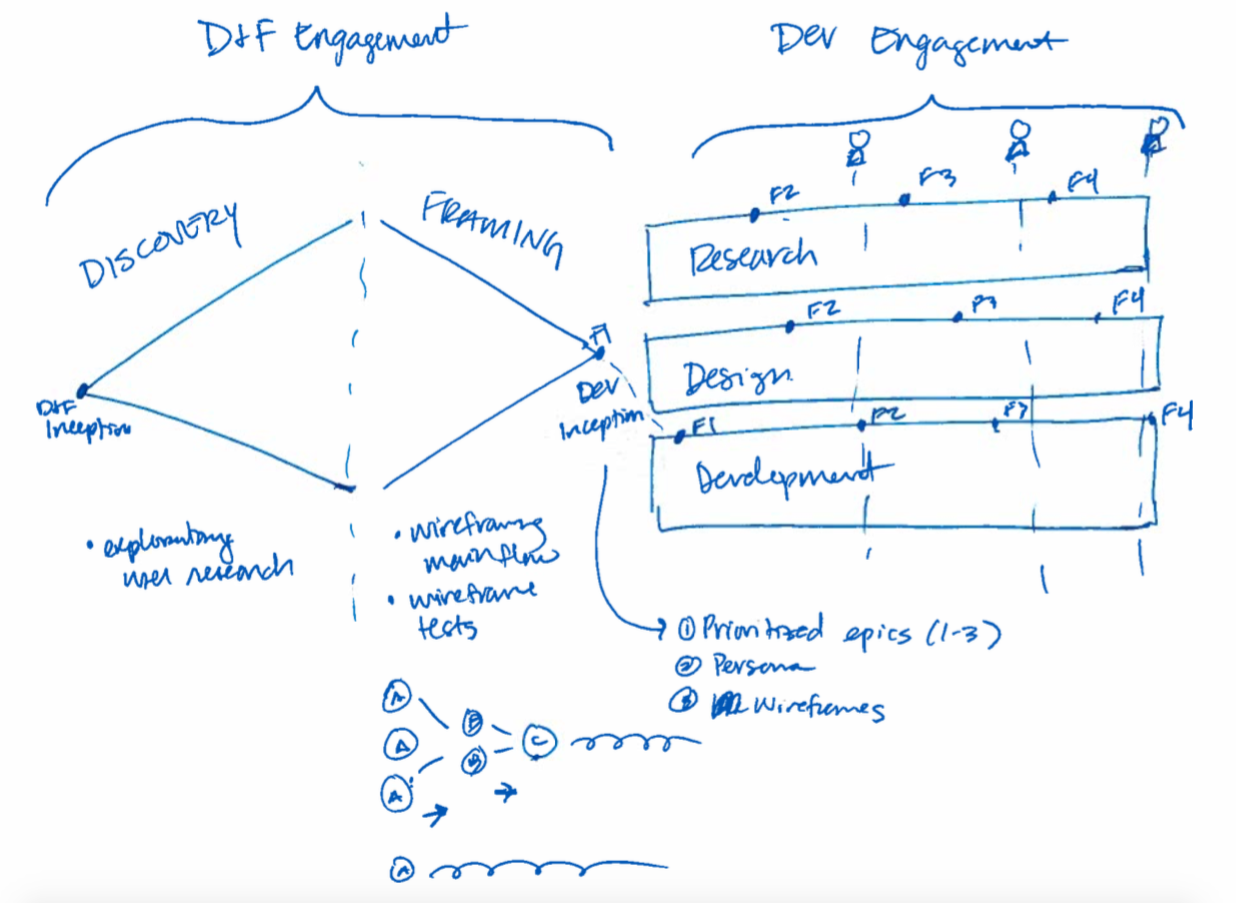
\includegraphics[width=6.5in]{interviews/drawings/2015_05_29.png}
\caption{\quotes{2015-05-29's drawing of a project work flow}}
\label{2015_05_29}
\end{figure}

\textbf{Interviewee:} Does it matter if there's a DNF first or...? 02:39

\textbf{Todd:} However you want it. Typical, ideal, however you want to draw it. 02:44

\textbf{Interviewee:} We actually show this to clients. We have this drawing here. 02:54

\textbf{Interviewee:} Most of the projects that I've been on start with the DNF. We'll call this DNF. 03:07

\textbf{Interviewee:} It's assuming the project has design in development going. This kind of, like, inception. 03:27

\textbf{Interviewee:} And this is dev inception. 03:32

\textbf{Interviewee:} This is your discovery, and framing. 03:50

\textbf{Interviewee:} Here in this area, we're sort of doing more exploratory research and sort of going wide trying to understand the users. That's something we do at the beginning of every project especially if the client doesn't know who their user is or they have ideas of who they are but it's not validated. 04:10

\textbf{Todd:} 	That's the discovery phase. 04:11

\textbf{Interviewee:} Yes. So, this is like exploratory user research. That's like interviews and maybe on site, shadowing people and things like that. And once we have a good idea of who they are, we start wire framing, maybe like the main flow and doing some wire frame tests like user research, that kind of thing and that's kind of within that, I think, we're kind of iterating as well. 04:45

\textbf{Interviewee:} I guess you can either start with one and iterate on that or you can start with many and narrow down. We've done both. So, when you start with many, you just- So, this is like your different As, research, then research to get to C. That makes sense? 05:10

\textbf{Todd:} It's like a portfolio of ideas? 05:14

\textbf{Interviewee:} Yes. I did it on my first project and it worked out really well and then from there you're kind of iterating on what you've come up with. 05:25

\textbf{Interviewee:} We came up with a couple, different nuance ways of doing something because they all seem good and they're like, two or three different features and we sort of combined them in different ways and then we took our insights from that and narrowed it down two versions, narrowed it down to one version. 05:46

\textbf{Interviewee:} I've also done it where you just start with A and you just iterate. I think both worked but this is fun to do. By the time we get to dev inception, we have prioritized epics. You have a develop persona. And you have wire frames. That's kind of the ideal for this point. At that point, development can start on say feature one and in the meantime, we'll start researching feature two. Then, we'll develop it. Then, feature three. So, it kind of goes like that. 06:37

\textbf{Todd:} Nice. 06:39

\textbf{Interviewee:} Maybe you have feature one here and then we'll go here. While they're doing that, we'll start on the next thing. So, on the next thing it flows down. I hate saying waterfall because I know it's the wrong kind. It's like a different kind of waterfall but it iterates in that way. So, we're like, \quotes{Oh, it's going in the cycle.} At any time, we're going to bring in users to test whatever we want. 07:09

\textbf{Todd:} You're drawing people. 07:12

\textbf{Interviewee:} Yes. These are users. At any given point, we can even do exploratory research. We can do wire frame or visual research or we can show them an actual prototype. 	It's kind of nice because you can, whenever you need people, whenever you're stuck on something, you don't have to wait for the right time to bring people in. 	It's just you can test anything at any given time.  07:34

\textbf{Todd:} Thank you. Have you seen a project that didn't quite fit this, what you've drawn here, this model? Or it was really different? 07:46

\textbf{Interviewee:} Yes. I was on a project. I was only on it for two weeks. It was just really quick enablement but there's basically no DNF. They came in with full visuals, full design. The problem is not a lot of it was validated. A lot of it was like, \quotes{Oh, the stakeholders thing. This looks nice.} 08:02

\textbf{Interviewee:} That was kind of different. As a PM, it was weird to write stories for full visual designs because I wasn't sure where to draw the line with the styling and things like that. We kind of had to feel it out. I think we stopped at colors and 	fonts. 	08:19

\textbf{Interviewee:} We did colors, fonts and a little bit of spacing for some other things but no animations, nothing like that. And that's also hard to convince the client, that maybe this isn't the right solution or things like that. I'm not sure how they got 	through without validation but it happens sometimes. 08:43

\textbf{Todd:} Do you think because it had such detailed mocks, they were married to their ideas? 08:49

\textbf{Interviewee:} I think so. It wasn't too hard, they're actually pretty open minded about stuff because they trust at our process. A lot of clients come in and like, \quotes{We trust you.} 08:58

\textbf{Interviewee:} For the most part, all the projects I've been on have been very flexible from that standpoint but I definitely felt bad for making the designer go through stuff. I don't think he minded but it's just a little bit harder to push back on things when they're not black and white and flexible. 09:21

\textbf{Todd:} Can you think of a different project that maybe didn't fit this mold in a different way? 09:27

\textbf{Interviewee:} Not out of the ones I've been on. They've mostly followed this. Like my first project followed this to a T. It was great. The second one just didn't have any discovery or framing. Right now, we kind of follow this as well. 09:51

\textbf{Todd:} I think given our sales process, we set this up for us. 09:56

\textbf{Interviewee:} You mean like non labs projects. 10:02

\textbf{Todd:} Just some labs. 10:02

\textbf{Interviewee:} 	Oh, just some labs. 10:03

\textbf{Todd:} Or in Pivotal. 10:06

\textbf{Interviewee:} Yeah. I haven't heard of any that- I think there are some enterprise projects that this doesn't quite work because there's an added QA layer. I haven't worked with a QA team but it just makes it harder to follow this because there's a QA layer that you have to go through in addition to acceptance. 10:28

\textbf{Todd:} In my current project, there's an approval process on designs and they want to see everything. You can't really do the features incrementally at least on design level. 10:40

\textbf{Interviewee:} That sucks. We have some design reviews. On most of the projects I've been on, we had weekly design reviews so nothing was a huge surprise to people. I guess I've just gotten lucky with the clients. They've been mostly receptive to our process. I hear horror stories about it but I haven't personally experienced any huge ones just yet. 11:09

\textbf{Todd:} As a PM, it feels like there's a lot that you juggle and manage. Is there one or two things that you remind yourself each day? What's the most important thing that you try to get right on a project? 11:26

\textbf{Interviewee:} If I'm working with a client, I always have to think about what I'm going to do with them. I think that's the biggest worry because I think any of the stuff I can do myself really quickly and I'll just remember things as they come up but I have to remember that I have to enable the client. 11:42

\textbf{Interviewee:} I have to be cognizant of what are we going to do today? What does the week look like? Not just the PM but I think PM in design especially during this period. It really helps to plan out the week just roughly and figure out okay, when are we doing research? What are some activities we should do? 12:01

\textbf{Interviewee:} There's some things you have to think about with the client from their perspective. Maybe they're not open to something. How do I convince them that this is the right way and try to put myself in their shoes and have empathy for them so I know how I can help turn them around to something that can work. Or help them come up with the idea. And I'm just like, \quotes{Oh you came up with this idea.} That kind of thing. 12:29

\textbf{Todd:} You mean you had the idea and you helped them realize the idea as well? Is that what you were saying? 12:35

\textbf{Interviewee:} Yes. We wanted them to go a certain way but they were like, \quotes{No we have to go this way.} How can we make them think that they came up with going this way. 12:43

\textbf{Todd:} It's like inception. You plant seeds. 12:45

\textbf{Interviewee:} Yes because they only listen to you so much. You tell people, \quotes{Trust me.} But they'll only trust you so much and then when they actually experience it, sometimes you just have to let people make a mistake and they feel that pain and they're like, \quotes{Oh okay. I will never do that again.} maybe not do that again maybe try this way. \quotes{Let's see what happens with that.} It's shows a different way of thinking. 13:12

\textbf{Todd:} What's it, for instance, on letting the client make a mistake and letting them feel that? 13:17

\textbf{Interviewee:} One time we had some clients who were very, very tight to us that are features and they call them core capabilities and very concrete and final and we kept trying to say, \quotes{Okay. These are assumptions.} They just didn't understand the word assumption. They're like, \quotes{No. We need to build these things.} 13:34

\textbf{Interviewee:} So, we did a couple of rounds of research because they weren't down for research. They never done that before and once they heard certain things, I think even though they heard certain things, their brain was still telling them they want these core capabilities. So, it's like they were, what is that called, like a confirmation bias or something like that or they're just like, \quotes{Oh yeah. That's what it means.} 13:53

\textbf{Interviewee:} And so, we did a synthesis and mapped out everything out and took their core capabilities and our main insights and tried to match them up. I think from there we could see that a lot of the insights didn't map to the core capabilities but it wasn't aggressive. We were all doing it together. 14:12

\textbf{Interviewee:} They were the ones making the mappings and saying like, \quotes{Oh. This moves down in priority. We didn't expect this to come up. Let's move on this first.} It took more time but it was nice that they came up with those conclusions on their own in a way or able to see that rather than us just telling them don't worry about this. Focus on the research. 14:37

\textbf{Interviewee:} You have to remember these clients come up with these things for months or years so they're very tied to them and to just rip them away from that is insensitive. I can empathize with them. You just have to have slowly validate or invalidate the stuff that they've been so closely tied to. 14:58

\textbf{Todd:} You described the client relationship and the parties you have with that. When you think about the development team, I'm biased, how to set them up for success, what's sort of things do you try and enable or set up for the team? 15:13

\textbf{Interviewee:} For the developers specifically? 15:15

\textbf{Todd:} PM. They're trying to make everything hum than what you imagine. 15:19

\textbf{Interviewee:} I keep communication really open. Before I start a project, if I can I like to talk to whoever is the anchor or the designer in the team and just get a feel for how they work with the PM because everybody's a bit different. 15:36

\textbf{Interviewee:} Big things that they would expect from a PM that I might miss or something like that and just try to get a feel for how they work with other people and obviously retro is great for a lot of that stuff. 15:50

\textbf{Interviewee:} Sometimes, we've had retros where we just talk about- because I think in front of the client you have to have a united front. And for the most part, in my experience, it's been great but if there are any disagreements or any problems, you don't want to bring up in front of the client it's really nice to have a pivotal retro. 16:09

\textbf{Todd:} How frequently might you have one of those? 16:12

\textbf{Interviewee:} Depending on how bad the project is. Once a week, maybe. Maybe once every other week. I don't know. 16:19

\textbf{Todd:} On top of the normal retro? 16:21

\textbf{Interviewee:} On top of. We have the normal retro usually and if we were at a point where we're feeling disconnected, we might have one. So, it kind of depends. I've never been in a situation where I needed one weekly. Although I've heard of those, really stressful ones. 16:39

\textbf{Todd:} Think of one of the worst projects you've been on, what's one thing you did to try and right it and get it back on track? 16:47

\textbf{Interviewee:} I haven't had any that were horrible. I think there was some bad times in my first project because the client wasn't committing to certain things. Once they went back to their own office. 17:10

\textbf{Interviewee:} We're working remotely and they were just being pulled into meetings. I think I was a little harsh. I don't know. I was just like, \quotes{Hey, the backlogs' drying, designing guys need to do stuff.} Because the devs were running out of things to do. They're just like, \quotes{What do we do?} 17:27

\textbf{Interviewee:} I tried to find other things that didn't require design to be prioritized. For that, I needed some help from the anchor because I don't have a formal technical background. 17:39

\textbf{Interviewee:} A lot of times I'll just ask. I'm like, \quotes{Hey, teach me this stuff.} Sometimes I'll have the devs say in stand-up that the backlogs' dry because I find the people listen to devs more than PMs or they take it more seriously. So, I'm just like, \quotes{Okay. You just say it.} I can say it 10 times but as soon as the devs say it, they're like, \quotes{Oh my god. [Interviewee] We're freaking out.} And I was just like, \quotes{Yes. I was freaking out two weeks ago.} 18:09

\textbf{Interviewee:} Sometimes you just have to be a little harsh. Just be like, \quotes{I know you have a meeting but we really need to move on this right now.} 18:21

\textbf{Interviewee:} I also paired with devs and designers which I think helped bring the team a little bit closer. The client PM was there half the time but I encourage him to pair sometimes. I really like cross functional pairing. 18:35

\textbf{Todd:} When you pair with dev, do you work on a story with the dev?18:39

\textbf{Interviewee:} Yes. I do whatever they're doing and I'm not necessarily coding from scratch but I know enough to recognize where things go. We'll type this in here or I might watch them do something then I'll do it. 18:52

\textbf{Interviewee:} A lot of it is discussion and asking questions. Like on this particular time, I had been on a project longer than the dev and so she wasn't sure where everything lived and I was like, \quotes{I think that data is over here. Can we do control+F for this keyboard} We're trying to figure out why something didn't work and I had a little more context so I was able to talk about it and she's like, \quotes{Oh. I know where that is. Let's try doing that type of thing.} It was a lot of back and forth. 19:22

\textbf{Todd:} Nice. I have not experienced that. 19:25

\textbf{Interviewee:} Yes. It's really fun. I love pairing with devs. It's also really intimidating. If you're at the helm of a spaceship or something and you're just like, \quotes{Oh my god.} but it's pretty fun. Everybody I've paired with has been really nice and patient and they like teaching. I was like, \quotes{Cool. Teach me.} 19:41

\textbf{Todd:} Pairing with designers makes sense to me, I think. 19:48

\textbf{Interviewee:} Yes. Again, it's a lot of discussion. Maybe we should put this here instead of there. I didn't know how to use Illustrator before but know I can poke around and use it. So, sometimes I get to do some stuff too. 20:01

\textbf{Todd:} That's fantastic. 20:03

\textbf{Interviewee:} Yes, it's really fun. 20:04

\textbf{Todd:} So, as a dev, sometimes I think about non functional requirement or they're called quality attributes. How do you handle those? As a PM, how does that work for you? Do you think about them? 20:19

\textbf{Interviewee:} You mean like visual design, thing like that? 20:23

\textbf{Todd:} Things like maybe performance or security or liability of the system. We call them ilities. There's like 20 of them that might show up in a project. 20:31

\textbf{Interviewee:} Yes. I think about them a little bit, honestly, in my experience here, at least. It's usually the devs or the client PM who is bringing it up. I should think about it more probably but when I think about MVP, it's like user mode but I think those get prioritized. 20:49

\textbf{Interviewee:} We just feel it out and honestly it's more of the client PM's decision and because they know the product better. If they're really, really lost, we'll try to make the most informed decision with them. 21:02

\textbf{Interviewee:} If we're about to launch or we want to do an initial release and obviously some of that stuff has to go forward. If some things, like really unknown or there's high risk, sometimes we try to write a story and just get that one story out there because that drives out a lot of the risk and drives out a lot of things that we might not know. 21:21

\textbf{Todd:} Trying to reduce risk makes sense to me. In my experience at Pivotal, I've not seen any stories about performance or things like that. That makes sense at some level because stories are about features. They're not about attributes of the system and I haven't seen how anyone here handles that. I'm curious... 21:44

\textbf{Interviewee:} I try to write all stories from a user perspective so I might say something like, \quotes{I want the spatial load faster because it's taking a really long time right now.} That kind of thing and so I know some places have requirements of loads in two seconds and things like that. 22:01

\textbf{Interviewee:} I haven't quite gotten down to that level but I'll still write it from a user perspective and if I have an idea of what might be slowing something down for example, I'll put it in there. \quotes{Oh, we have a page full of SVGs maybe we can convert them on to PNGs or something like that.} I try not to be too prescriptive because that's just not my place. 22:24

\textbf{Todd:} Good. 22:27

\textbf{Interviewee:} I try to handle them from the user perspective as much as possible. 22:30

\textbf{Todd:} I have created a little model for stories. This is now called described or something. Defined. 22:44

\textbf{Todd:} From your perspective, this is a flow of stories, give me feedback for me on those. 22:53

\textbf{Interviewee:} Named is just identifying the story. Once you flush them out and written them and they've been through pre-IPM and they're estimated, they're started, blocked. I usually don't go back and estimate. So, it's like this. 23:12

\textbf{Todd:} It could happen. 23:13

\textbf{Interviewee:} I usually don't do this. I guess it depends on what's happening here. I haven't re-estimated a story unless we pointed it five weeks past and then it comes up in the backlog, we might revisit it and say, \quotes{Okay. Do we still think it re-points?.} 23:35

\textbf{Todd:} Well, we try not to re-point. I agree with that. 23:37

\textbf{Interviewee:} I haven't done that. Started, finished, delivered, accepted. 23:42

\textbf{Interviewee:} Delivered. Checked in. This would go back to - Oh, you have that here. Delivered. So, when will it go from delivered to started?  23:56

\textbf{Todd:} The irony is this actually comes form tracker data, this graph. I went through a ton of project and watched all the transitions of every story and there was a story from delivered to started. 24:08

\textbf{Interviewee:} Maybe they delivered on accident? That sometimes happens. Or was it delivered on purpose? 24:14

\textbf{Todd:} I think what happens there is you deliver it and then you realize there's more work to be done. 24:19

\textbf{Interviewee:} Oh, so the dev will go back and... 24:20

\textbf{Todd:} Say, \quotes{Oops. We're not done.} 24:23

\textbf{Interviewee:} Okay. 24:24

\textbf{Todd:} Or someone will walk by and say, \quotes{That's not done. You didn't do X.} 24:28

\textbf{Interviewee:} Just like  before the PM hits something, they'll say, \quotes{Hey, you guys, forgot this.} 24:32

\textbf{Todd:} It's kind of like the rejection where the PM didn't reject it. 24:34

\textbf{Interviewee:} That makes sense. I've done that before. Finish, delivered, accepted. 24:40

\textbf{Todd:} That has happened, believe it or not. 24:47

\textbf{Interviewee:} Really? 24:48

\textbf{Todd:} I agree with you, the ideal is that would not happen. My point in showing this is to actually help you make sense of what I'm about to show you next. This is my view of stories. 24:56

\textbf{Interviewee:} I've been trying to create a checklist items for each state that the story could go in. I just wanted you to look at this list and see if you have any... 25:06

\textbf{Interviewee:} The idea is, for something to be named how do you know it's named or not and these would have to happen for each state. If this is not clear, ask questions and I'll try and clarify. 25:19

\textbf{Interviewee:} Okay. I think this is like an either/or. It could be prioritized or it could not be. Can we write down? 25:34

\textbf{Todd:} Sure. Whatever you want. 25:36

\textbf{Interviewee:} Defined. Feature is prioritized. I think this can also be either/or. 25:45

\textbf{Interviewee:} I usually don't prioritize until - I'll have a rough priority but I'll wait until they're all flushed out. Sometimes in pre-IPM even they're not fully prioritized by this time. Usually after they're estimated, usually they're prioritized but sometimes after they estimate, I'll rethink some things. 26:13

\textbf{Interviewee:} If they're not fully prioritized, that's okay. 26:16

\textbf{Interviewee:} Story describes clear acceptance criteria. That makes sense. That makes sense. 26:22

\textbf{Interviewee:} Story only describes user interaction with system. Yes. I think some people do this. I really like to do this. Oh, ideal PM. 26:33

\textbf{Todd:} That's your ideal. 26:34

\textbf{Interviewee:} Yes. 26:35

\textbf{Todd:} It doesn't have to happen. 26:35

\textbf{Interviewee:} Yes. Business value is clear. Yes. I'd say, relevant. Did you already write that? 26:59

\textbf{Todd:} No. I did not. 26:59

\textbf{Interviewee:} I try to attach design to every story. I try not to write a story before a design is done and that works out really well. And that's kind of the ideal. 27:09

\textbf{Interviewee:} Estimated. Feature is estimated. Nothing blocks developers from working on the story. Yes. I would even make this required. 27:24

\textbf{Todd:} I've estimated stories that were blocked that's why it's ideal. So you feel strongly about that. 27:34

\textbf{Interviewee:} If it's blocked, I don't. 27:36

\textbf{Todd:} Why do you estimate it? 27:37

\textbf{Interviewee:} It's not going to be accurate. I guess there are some stories where the devs are kind of like, \quotes{Well, I've never worked with that before.} If something's not defined or this is clearly blocked then I'll probably be like, \quotes{Okay. We'll just wait.} 28:00

\textbf{Todd:} Would you say it would be okay to estimate if you're trying to figure out when the end of the project is going to be even though things might be blocked? 28:06

\textbf{Interviewee:} Yes. I can see doing that. I've heard of that. I haven't don that on a project yet but I know they've been pointing  parties where people do small, medium, large type of thing or really rough pointing estimates. I think that's fine but for an IPM when you're going to work on something ideally, it's not blocked. Started. Yes. Blocked. It depends to you. Yes. I think that makes sense. I can't speak to these two. 28:37

\textbf{Todd:} You've paired on code so you might have more of an opinion on that than other PMs. 28:45

\textbf{Interviewee:} I agree with it. It makes sense. It was funny, I was pairing with somebody and we were working on an iOS project but it also involved JAVA and so we had, was it C\# or not C\#, what is it? 28:58

\textbf{Todd:} Objective C. 28:59

\textbf{Interviewee:} I guess she's more familiar with Objective C and not JAVA. She's kind of like, \quotes{Oh. I don't know Java that much.} She was like, \quotes{It all looks the same to me.} It looks equally confusing. 29:15

\textbf{Interviewee:} Units test pass, makes sense. Acceptance passes. What is the difference between a unit test and acceptance test? 29:28

\textbf{Todd:} Unit test are the very low level. They test one thing in isolation. Acceptance test, they're more PM level. Does the feature do what it's supposed to do? Does the story work? 29:42

\textbf{Interviewee:} So, the devs will do an acceptance test. 29:47

\textbf{Todd:} Sometimes they have them sometimes they don't it depends on the project so I'll probably put ideal or optional on there as well. 29:51

\textbf{Interviewee:} Is that something actually written or is that more of like the devs going through what they acceptance criteria says? 30:02

\textbf{Todd:} It depends on the project. Some of them we will write acceptance test. 30:08

\textbf{Interviewee:} Code reviewed prior to commit. Changes reviewed prior to commit. That makes sense. Delivered. Yes. PM updated the acceptance criteria because they were not clear. 30:28

\textbf{Todd:} You're going to fill out some of these. Go ahead keep going. 30:32

\textbf{Interviewee:} I do some of these things. Additional requirements that need to be implemented. The PM changed the requirements and the codes need rework. This shouldn't happen. This shouldn't happen. This shouldn't happen. 30:50

\textbf{Todd:} I completely agree with you. 30:52

\textbf{Interviewee:} If the PM changes their requirements, if it's small, sometimes, I'll say, \quotes{I meant this but I forgot to put it in.} If it's really tiny, they're like, \quotes{It's okay we'll just do it.} I'm like, \quotes{Okay. Thanks} 31:03

\textbf{Todd:} Why write another story. 31:03

\textbf{Interviewee:} Yes. And I'll just put a comment. I'll say, \quotes{It works but I forgot to add this.} So, devs rejecting so you can add this thing or something like that. But if it's something big, I'll be like, \quotes{Sorry, I forgot that.} And I'll just write another story. I'll be like, \quotes{Let me just write another story.} 31:23

\textbf{Interviewee:} Sometimes I'll write a bug and I don't have a clear criteria when it's a bug and when it's an extra feature but in the moment it makes sense. I just can't think what I used to decide it's a bug or not. 31:38

\textbf{Todd:} I know what I use. 31:43

\textbf{Interviewee:} One time, we were building something where you can adjust the quantity in a card and we were like, \quotes{It has to be an integer. it can't be zero.} And we were able to add zero and we were like, \quotes{We shouldn't be able to add zero.} That was a rejection but the fix they made, it had to be applied to this other scenario that wasn't covered in the story. But since they did it for one, \quotes{Okay. Let's just create a bug for it.} Because it was treated as a bug in the other scenario so it's kind of like a weird scenario. 32:21

\textbf{Todd:} For me, the black and white description is, if the story says it should do something and the code doesn't, that's a bug. If a story doesn't describe that condition, then it's a new feature. 32:32

\textbf{Interviewee:} Yes. 32:34

\textbf{Todd:} There's probably a gray area. 32:36

\textbf{Interviewee:} Yes. There are some gray areas where you decide should I reject it or should I write a bug type of thing. I think, definitely, in that first scenario, it's either reject a bug or usually that would just be a rejection because it says it should do this but it doesn't. 32:49

\textbf{Interviewee:} Anything additional should be another story but sometimes I do a bug instead of a rejection for some reason and I think it's for little things. PM updated the acceptance criteria because they're not clear. That sometimes happens. If it's small. So, I'll say, if it's small. And sometimes when I reject something if it's really nitpicky, I'll put nit. Do you guys do that? 33:18

\textbf{Todd:} What does that mean for you? 33:21

\textbf{Interviewee:} I don't know. A dev told me to do that one. I think it stands for nitpicky or nitpicking. I don't know. Sometimes, I'll be like the word is off or something. Technically it can go out but it should have this other word or the color is a little bit wrong and I'm just this works perfectly but I'll say it, nit. 33:44

\textbf{Todd:} So, in the comments of the story, you will put nit:fix this. 33:51

\textbf{Interviewee:} Yes. I feel it's a little nicer. I don't know. It's just like nothing's wrong, it's just the mock has this and it's a UI type of thing. A Dev told me to do that once. I was like, \quotes{Okay. I feel better about doing that because I feel bad rejecting stories that are technically work but just have a weird...} 34:10

\textbf{Todd:} I think I've seen one PM not accept it and put a comment on it,  which notifies people and then they would accept it once it's fixed. But rejection is probably the right flow. 34:22

\textbf{Interviewee:} Yes. If it's not rejected, you're not going to see it. As a dev, I would imagine. QA manager added new requirements. This should happen. I just think that's so silly but I guess some big companies have a QA process but they should not add new requirements. They should be bugs features and then... 34:55

\textbf{Interviewee:} I've had QA say, \quotes{Oh, this doesn't work.} or \quotes{This has this one case it won't take a credit card after 2049.} I was just like, \quotes{Okay. Let's write a bug} but I just put at the bottom backlog. We'll put them in the backlog but the PM will prioritize it as they prioritize everything else. That shouldn't lead to a rejection ever. 35:17

\textbf{Todd:} Given everything that we talked about in this conversation, is there anything else that you think would be relevant? Maybe questions I should ask? 35:26

\textbf{Interviewee:} What is your objective? What stuff do you want to know? 35:31

\textbf{Todd:} I should have a clear answer to that question. I think at this point, I'm really curious how what we do differs from what Kent Beck described 15 years ago. We've done a lot of really neat things and so I've been really interested in that. And I have a question I'd prefer to ask without leading it. Why do we call an IPM an iteration planning meeting? 36:10

\textbf{Interviewee:} Versus? 36:13

\textbf{Todd:} Why do we call it that? There's things that we do in the meeting and does the name describe what we do in the meeting? What's the purpose of an IPM? 36:27

\textbf{Interviewee:} It's so the team is aligned in what we're going to be doing for the next iteration or the next week. I guess, sometimes, the things that you point in IPM don't always line up to what you're going to be working on in a week. Sometimes, we'll end up pointing a lot of things. I think it's a good way. I think ideally, it is supposed to spell what the team is going to be working on for the next week or the next iteration. 36:54

\textbf{Interviewee:} So, you know you have immediate contact. You just pointed it. You know exactly what's happening. There's not a lot of time between for you to forget. Most of the time it happens or at least you'll start working on some of the things you pointed on that week but I think also it's a good rhythm setter for the team like you meet every week and you feel like you have this check in. You're always connected. You have frequent connections with dev and PM and design. Because I think PM and design can be off. We're usually ahead, design especially but PM, kind of split but we have fear what's going on right now and also be two weeks ahead and so I feel like this helps bridge the gap between what's going on in the design world and the dev world and having those check ins really helps 37:48

\textbf{Todd:} For me, it's like weekly estimation meeting. About six months into my career here, I realized that, for me, in my perspective there is no iteration. We do retros on Fridays because Mondays we don't remember what we did last week. We do weekly estimation meetings somewhere in the middle because we need to have enough work. The worst thing that could probably happen is I have six devs with nothing to do. So, we need to make sure that there's enough of a backlog for them. I was on a project where I had no idea that iteration started on Tuesday. And that was the clue for me. What? Are there iterations starting on Tuesday? I had no idea. 38:28

\textbf{Interviewee:} So, what do iterations mean for you then? 38:31

\textbf{Todd:} I think there is no spoon. I think it's a very kanban-like the work flows through us. The team isn't committing to a scrum that says, next week we're going to deliver these three features. 38:44

\textbf{Interviewee:} Yes. I can see what you mean by that. I feel that way, too, sometimes. 38:49

\textbf{Todd:} I think that's great. We show up and we do where the work is needed. 38:54

\textbf{Interviewee:} Yes. 38:56

\textbf{Todd:} So, halfway through a week something in the universe completely changes, we respond to it and start adapting to it. It's not like there's this ready plan. On Friday, we're going to launch this feature. We can't do that. In the original definition of XP, the team was committing to where they will be each week. 39:16

\textbf{Interviewee:} I didn't know that. 39:17

\textbf{Todd:} Yes. 39:18

\textbf{Interviewee:} I had no idea. I thought XP was totally. 39:21

\textbf{Todd:} And you couldn't change what the team would do that week? It was inflexible. 39:24

\textbf{Interviewee:} That's against everything that we do. I actually didn't know that and I read the XP book. 39:30

\textbf{Todd:} If the PM changed what they did during the first week, there was a contract violation between you and the team. 39:36

\textbf{Interviewee:} That's so crazy. I need to go re-read that book or something because I totally have been telling clients XP is flexible. 39:41

\textbf{Todd:} and..with XP..what we do here. That's really interesting. 39:45

\textbf{Interviewee:} Yes. That's kind of how I see it. I think, if anything, it gives a team a rhythm. I think retros help us sort of figure out what didn't go well during the week. What we need to change so it's not at some arbitrary point somebody might say, \quotes{This isn't working. Let's try to figure out how to change it} There's a forced check in so anything that you think you had a problem with this week, you know we'll come up at least every week and then you can do something to make the next week better. I think, work flow wise, maybe we're not doing things iteratively but team-cadence wise, we have iterations of like, Okay. Let's take an arbitrary piece of time. A day's too short, a month is too long. So, let's do a week. Just make sure there are teams running smoothly every week. I think it serves that purpose maybe more than the actual delivery and execution. It's more about the team spirit, I guess. 40:59

\textbf{Todd:} I think what I'm hearing you say is, your view of the word iteration might be different than mine and so you're happy to call in IPM because, for you, it's this weekly rhythm that's maybe artificial because of weekends. If there were no weekends, we might have a different rhythm or something 41:20

\textbf{Interviewee:} Yes. 41:21

\textbf{Todd:} It wouldn't be healthy 41:22

\textbf{Interviewee:} Yes. I think it's like a force check in because we were just to do things. We think about things in terms of time and so if we didn't have a time marker I think we would just get very confused and we would get very lost in what we're doing. 41:40

\textbf{Interviewee:} And even new devs are estimating stories, they still want to estimate in terms of time. We're always thinking in terms of time because that's how the world works in a way and so I think having that time marker helps us keep things in check versus if we just let them run on forever. 41:58

\textbf{Interviewee:} So, yes. I guess I think about iterations. I haven't thought about this deeply before but I guess me, for iterations, it's more like the team rhythm and team cadence versus the actual execution of things. 42:09

\textbf{Todd:} Yes. Okay. 42:11

\textbf{Interviewee:} I guess iteration in context of how we use it here. 42:14

\textbf{Todd:} That's very helpful for me. I'll have to deep think on it some more. 42:18

\textbf{Interviewee:} Building iteratively I think it means something else. Like what I was saying in the beginning, you just start with the first layer and the second layer. That's a little bit different than what I'm thinking in terms of team iteration if that makes sense. 42:31

\textbf{Todd:} It does. I don't have anything else. Is there anything else you wanted to share or anything you're not telling me? 42:40

\textbf{Interviewee:} I don't think so. I've worked in waterfall before so this is like a huge breath of fresh air. I think it's much healthier. I think the ideal of what this is supposed to be is good but it's not always applicable especially with enterprises, for example. We've definitely had to bend a little bit more to work with enterprises because it's just not the solution for everybody. You have to cater a little bit to different types of organizations. 43:19

\textbf{Todd:} I forgot about demographics. How long have you been at Pivotal? 43:21

\textbf{Interviewee:} I've been here almost a year. I started in August. 43:25

\textbf{Todd:} Just in terms of your career, when did you graduate from college? 43:31

\textbf{Interviewee:} 2010. 43:32

\textbf{Todd:} Great. That's it. 43:33

\textbf{Interviewee:} Okay. Cool. 43:34

\textbf{Todd:} Thank you. 43:34

\textbf{Interviewee:} Yes. Thank you. This was fun. 43:36


% \section{2015-08-12 Anchor Interview}

\begin{figure}[h]
\centering
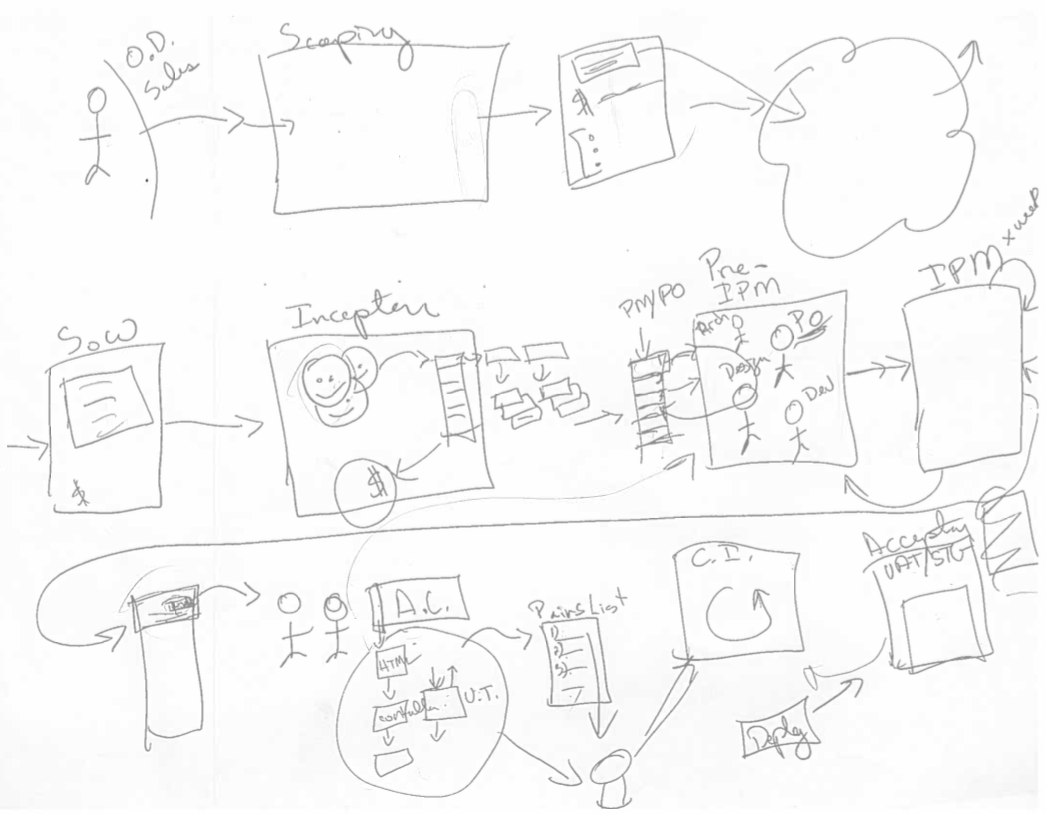
\includegraphics[width=6.5in]{interviews/2015_08_12_anchor.png}
\caption{\quotes{2015-08-12 Anchor's drawing of software development process}}
\label{2015_08_12_anchor}
\end{figure}

\textbf{Todd:} 	So on a sheet of paper, curious could draw your perspective on our process for software development. 0:00:09

\textbf{Interviewee:}  	Our process for software development.  Where do you want to begin?  Or is that like…  0:00:14

\textbf{Todd:}   Really open.  0:00:15

\textbf{Interviewee:}  	So there's a customer, a potential customer.  And they come and there's some kind of vetting to, at least, get them in the door.  We think that they have interesting idea of some kind, and maybe we ask a couple of questions; so this might be the OD or sales.  Just some minimal vetting and then just enough for them to say: \quotes{you know what, I think we could possibly have a conversation about what it is that you want to have built.}  So then we do a scoping with them, and in that scoping, the input is their general idea.  Usually, it's like pretty vague; It could be from very vague to they totally know what they're talking about both on their problem space and with the solution to look like.  So then the output of that is a document that basically tells them this is what it likely is, and this is how much it's gonna cost, roughly speaking, and these are gonna be the roles and responsibilities, this is what you would be buying.  What just really actually, some amount of hours of some amount of people, different skill, that's what we're actually promising and we'll aim for this thing, but we'll always constantly trying to give you the best value thing as we go along.  So that's some kind of proposal, I don't know exactly what we call that, but it is all part of the scoping.  0:02:00

\textbf{Interviewee:}   And then, I'm gonna draw, like, maybe a number of stops here; by the time I see it, somebody signed, like, an SOW or similar that was possibly, like, but influenced by that scoping value but who knows what negotiations or whatever happened after that; and probably informed by that document, like, what we say we're aiming to deliver.  But this is, I think, this is more like a legal document or as the SOW is more like a legal document whereas the thing that came out of scoping is more of like a \quotes{come work with us} and some of the other stuff around that.  So then, we go into an all of these assumes it's ok.  I'm talking happy path.  Cool?  0:02:59

\textbf{Todd:}  	Yeah, I'm good.  0:03:00

\textbf{Interviewee:}  	So then we do an inception, and this is where, regardless of what we said over here, we get them to get really clear about who is the person that they're targeting; like, ok so it's about a product market fit, who's the market, what's the product gonna be.  So here's this person or persons or personas, and then for each of one those, like, what are the kinds of things that they need to get done, right?  So they've got things that need to happen, that ultimately will result in to some kind of outcomes, and it almost always like it's gonna convert to dollars in some way, shape, or form.  Sometimes it's a non-profit thing and that's slightly different, there's mixed motivation.  So then what we do is we say, \quotes{ok, in order to meet those tasks, what we need is features from the product} and so we're calling out, like, epics, if you will, feature sets, whatever, and then when we start breaking those down into individual stories and these are just sketches at this point.  We're not gonna get all into acceptance criteria right away, it's just like trying to enumerate coz really the outcome of the inception is a backlog. 0:04:43

\textbf{Interviewee:} So you've got some product owner, who culls the outcome of that into a prioritized list of stories, each one of those describes at tiny interaction between this person and the software that we're building.  Ideally, there's variations on that but then, so that's what an individual user story is.  0:04:58

\textbf{Interviewee:}   And then we go to kick off.  So then, we have our first iteration planning meeting where we take as input the prioritized backlog and for each story we go through them.  And by then, the product owner has got them into a point where I call it readied, they've met the definition of ready, which is they have clear acceptance criteria.  There might even be, a pre-IPM where that work is done, as well as, so this is the input is the backlog and the output is the backlog in the pre-IPM.  There are two things that happen, one is that we get clarity early on what the requirement is, and the other is that we get technical input to help with that prioritization and viability, like, ‘ok this may seem simple, like on the face of it', but actually, there's a whole of things that has to happen to make that work, etc. So we surface some of that, the pre-IPM includes somebody from the product side of the house and someone from development, so product owner, development.  Sometimes depending on those, the story can get more complicated, the more requirements, with the greater the variety or the more exotic the product is.  So you might even need someone in from design who is kind of help guiding how this should unfold and the interactions between things because there's all kinds of decisions from that end.  I Imagine, although, we haven't done this yet, in an enterprise client that you might even have somebody from like architecture there, business architecture.  The point of this conversation is to get all of the perspectives that need to be folded into the prioritization and the validation of, that the stories are legit.  0:07:11

\textbf{Todd:}  	Yes.  0:07:12

\textbf{Interviewee:}  	So then that goes into IPM, and this is a straight-forward roll through - the from top to bottom - the backlog, and we go over each story.  We read out title, we read through the acceptance criteria and then the team points each of the stories, the purpose of that is to surface complexity and to get a general, like, understanding, like, common understanding of what this thing actually is, what it is, what's gonna be involved to building it.  0:07:52

\textbf{Todd:}  	Yes.  0:07:53

\textbf{Interviewee:}   	We don't give in to like, we try not to give in to implementation details.  Sometimes, we have to dip down for a second to like verify that we're all speaking the same language, that we're all really envisioning the same kind of thing.  But that usually is surfaced by like, \quotes{I pointed at one and you pointed at five,} and then I would like \quotes{what?}  So then that hopefully prompts a conversation.  If we all said three, it's good enough for now we move on, if we all think it's about the same thing and the product owner doesn't lose their mind hearing that number, then we're all kind of okay.  Then the output of the IPM is individual points on the stories, and we typically go for some amount of horizon so the minimum that I feel comfortable walking out with is at least for the week, so we don't have to, like, break the flow of getting work done before the next IPM because we're gonna do this once a week, these IPMs we're gonna do this once every week. But ideally, a little bit more runway so that we mitigate against that the team haven't jumped out of the flow and also to, like, help the product owner have some room to sort of steer.  If they only have so many points in the stories, then they have to kind of pay the price of reprioritizing. So that's IPM.  Haven't have written a line of code yet.   So then, after IPM, we get working. So out of the backlog, a pair picks up a story and so then that pair looks at the story...  How deep do you want me to go, because I can go all the way down to like testing and stuff.  0:09:48

\textbf{Todd:}  	Sure.  0:09:49

\textbf{Interviewee:}	Ok.  0:09:50

\textbf{Todd:}	This is your diagram.  There's no wrong answer.  0:09:54

\textbf{Interviewee:}  	Alright. Ok.  So, the pair looks at the acceptance criteria and they say, \quotes{hmmm.... what test do I need to write that will help?  Or a set of test that will help if those tests ran green?  I feel really confident that we've met the spirit of that story.}  So they start there.  Usually at pivotal will do typically outside in so that means if we write something that looks like an acceptance test, something that describes very closely what this person with the persona experiences both in what they do, and what they see back from the software.  So we write the starts, we start with a very low fidelity version of that. It's not gonna describe the whole interaction, it might describe the smallest piece of we could possibly articulate; so we start there.  And then we run that test and it fails.  Then we say, \quotes{hmmm, ok, so we're in this architecture, what's the next part that we need to build in order to begin to meet those needs?}  And we work our way down the architecture.  In a typical web app, there's something that's displaying, an HTML page, and then there's something that is probably orchestrating the generation of that HTML, like a controller and usually we try and separate our concerns. We think about these things as we work our way down driven by trying to meet just this one acceptance test.  0:11:26

\textbf{Interviewee:} So along the way what we do is we write individual unit test for the components that have interesting behavior.  The controller does have interesting behavior.  It takes in some input and it makes some decision about what should be the output, what should be the resulting HTML.  And that controller also interacts with other collaborators.  So we have tests that say, are you properly handing off these parameters?  So these really fine-grain unit tests. But the key is that these things are, each time we write these tests, we're setting an expectation on that little tiny piece of the system, in the same way that our acceptance criteria are setting an expectation on the software, and our user stories are setting expectations on the feature .  So forth, all the way back up. We're trying to be needs-based  all the way down as we do this; that's probably good enough.  The details of how that happens varies wildly and even like within this, there are different schools of thought about how that happens.  There's people who believe in writing units for every little thing and people who say \quotes{no, you can set certain bullwarks} and write tests around the bullwarks.  Let everything sort of float in between.  0:12:43

\textbf{Todd:}  	It's a whole like, Chicago versus London.  Like, on how much mocking and doubles do we have?  0:12:49

\textbf{Interviewee:}  	That's right.  0:12:50

\textbf{Todd:}  	How much more integration of the unit test level do we have.  Are we really testing real things or not.  0:12:55

\textbf{Interviewee:}  	Yes, exactly.  0:12:56

\textbf{Todd:}  	Yeah.  0:12:57

\textbf{Interviewee:}  	Exactly.  So and the other part, too, is I think a factor in there in the choices that I make about these things, have to do with who the team is.  On like what their level of experience with test driven development is, and if it's really, really low, then I'll tend to want to have them write many more unit tests.  And I know that that is more fine grain tests, I know that that's harder at first but then they more quickly ramp up because they have more guard rails around them to guide them along their way, as they're learning the knack, the feel, the tacit experience of being test-driven.  Then as they start to become more comfortable, we can back off a little bit on some of these unit tests; especially if they're not catching anything, so test have a shelf life and if they haven't caught a defect, then there's a question of whether or not it's actually carrying its way.  So that can be a way of starting to prune part our of test system.  0:14:10

\textbf{Todd:}  	There's a bunch of people who are concerned about declarative tests or tests that test declarative code.  0:14:16

\textbf{Interviewee:}  	Ooh. Yeah. 0:14:17

\textbf{Todd:}  	Do you worry about that when you're thinking about this?  Difference is Rails has a lot of configuration and it's like why test the configuration when we already know that Rails works.  0:14:26

\textbf{Interviewee:}  	Right.  0:14:27

\textbf{Todd:}  	And that's through another framework to like... 0:14:30

\textbf{Interviewee:}  	Yeah.   0:14:31

\textbf{Todd:}  	Or does that not really end, you just like, \quotes{hey, let's just test everything?}  0:14:34

\textbf{Interviewee:}	 No, it does matter.  And I don't know that I have like a pat answer.  I think I'll probably flip flop depending on my mood and who knows what else.  I think if it's something where it is like a one-time configuration, so some of the factors are “how often are we gonna touch this;”  “how bad is it if we get wrong?” If it's like important plumbing that could get broken later on or something like that.  Coz you can do bindings, right.  Like bindings are kind of declarative piece so you tests those.  So I'd start off probably testing that kind of stuff.  But I'm not gonna test to see that configuration params are correct.  0:15:36

\textbf{Todd:}  	Because presumably it won't start up if they are wrong.   0:15:40

\textbf{Interviewee:}  	Exactly.  0:15:41

\textbf{Todd:}  	I interrupted you.  Did you finish with your diagram to the very end of the story?  0:15:45

\textbf{Interviewee:}  	So we get through the story, and then there is more to this process here.  As we go along through this development, some things feel easy and flow well and some things don't; and the things that don't, they go off on, what I call a pain's list, and I learned this from George Dean.  The idea is that let's enumerate things, let's just quickly note things that are challenging.  We may even have to work around them, like, \quotes{ah I want to take this certain tack but I can't,} so we note it.  And then, what I'd like to be able to do is get to the point where I can click finish on my story in Tracker.  But before I do that, when I feel like I've met all my acceptance criteria.  All my acceptance tests have met the acceptance criteria, then we'll stop as a pair, we'll quickly triage this list, some of the items just suck and we're not gonna do anything about it right now.  It's probably just, it's something that, it's not worth calling out as a chore yet. Or maybe it's too big, too; or maybe now after having gotten through the story, maybe we've changed our mind, maybe we have different perspectives, something like this.  We'll do one of three things with it, one we'll either address it right now, like \quotes{you know what, this is a two-point story and my god we flew through this, it took us an hour or two. Let's say we've been tracking a little bit longer for those kinds of stories.}  I feel like I have a little bit of buffer in terms of raising the quality dial a little bit so we'll address a pain.  What we're trying to do is hit the thing that's gonna be the least of effort for the most bang. We're looking at things, there often things like, it's all about maintainability, making the software more of an asset than an expense.  So readability, where there's something that's different for no good reason, bringing that back in line, all those kinds of things, so we'll address it - that's one option.  Two, we say, we're not gonna address it now but it's pretty important; it's one of those things where this is really gonna bite us if we don't do something about this or it's gonna create a ton of back flow where we will be blocked a whole bunch of stories if we don't address this soon.  So we'll mark it as a chore.  Or three we say, \quotes{yuck, don't like this.  It isn't necessarily gonna bite us right now, and if it really is painful, we're gonna discover it again}, so we delete it.  We try to empty our pains list and that's the last step and then we go and we click finish.   0:18:49

\textbf{Interviewee:}   As a part of clicking finish, either, and I've seen this in many different ways, either it's automatically hooked up from our version control system in our CI, we have a CI box, some CI setup that's listening to the same repository that our code is going into and it kicks off a build and when we commit with a certain message, it will mark it as, it will click the finish button for us effectively, finishes and then the tracker story number.  0:19:33

\textbf{Interviewee:}   Meanwhile, and this next step might have happen as a part of this whole development process. As long as everything is running green, I could actually commit and I'm not delivering a feature that couldn't be deployed, so maybe partial but if it's not seen, then it is ok.  So anyway, my point being that, we have a continuous integration server that acts like the nth + 1 developer on the team.  So it goes and it fetches the code just like the developer would.  Actually, the initial version of this was called integration station, where it was literally a box at the end of, like an end cap on a team's desk, and you'd get done, and you'd walk over, you‘d manually do this process.  And now it's automated.  The point being that we're demonstrating that the code can be built from scratch reliably from master.  Which means it's included in everybody's work up to that point and then all test runs. 0:20:39

\textbf{Todd:}  	Nice.  0:20:40

\textbf{Interviewee:}  	Ok so when we click finish, we see the CI build go green, then this varies also wildly.  We wanna deploy to some kind of acceptance area; so maybe it's called UAT somewhere, sometimes it's called staging, whatever it is.  So it's a non-production environment that now, the product owner can go and vet that feature against the story, thinking about this person and getting their job done.  So that can either be accepted or rejected; if it's rejected, then it goes back into the backlog.  And then, I didn't really make enough room for this.  0:21:34

\textbf{Todd:}  	If you need to use a second sheet, you can.  0:21:36

\textbf{Interviewee:}  	Ok, Cool.  So let's go like this.  So that's where the acceptance happens.  And then time passes, so we go about for a week and then we get together as a team and we dead reckon, at the end of the IPM, it's almost sort of like we all sort of have an idea about where we're going and what we think we're gonna accomplish.  0:22:02

\textbf{Todd:}  	Yes.  0:22:03

\textbf{Interviewee:}  	And then wind and weather, like, affect our actual location where we end up, so we need to, as a group, see where we're at, both in terms of progress we've made in development of the product and what we've learned along the way in terms of working with each other, and the technology that we're using, and what we've learned about the product and all these stuff.  It's navigating in all these dimensions so that's what the retrospective is about.  And so there, we step out of getting things done mode and trying to into a mode of dis-identifying that and reflecting on the process.  And we have kind of a pat way that we sort of do it at pivotal, there's a lot of different ways to retrospect.  But we focus typically on emotion-based sense-making.  So we say, what makes you happy, what leaves you sort of neutral, what might make you angry or frustrated or whatever.  That's a terrific way of getting an idea about, like our emotions are a really good way of developing situation awareness so we're gonna have one way of doing it, it's probably the best way that I would know of.  So we just throw up a happy face, a middle face and a frowning face up the board. We have people register anything. You could just be having a catharsis in front of the group, that's fine.  The point is to try and make some sense of what just happened just this last week.  And ideally, we come up with action items; and these could be in the form of what actual people do, so \quotes{oh, so and so needs to add a chore,} or we need to change this like about how we, the time that we do our stand-up or something like that, or they could be team agreements, so we clarify what the definition of done is.  Don't click finish until you see it, you smoke it yourself in the staging area before you hand it off.  Or please include instructions in the user story about how the product owner should accept this.  Some sample data or whatever it is.  We come to try, we looking to continuously try to improve as a team.  And that's the moment where that happens.  And then ideally, you kick the whole process off by jumping back into an IPM away we go again. Ideally, along the way, in parallel, this collective, this little mini team here is keeping the backlog groomed, looking ahead trying to think about, again, dependencies to both end.  What's important, what needs to get done in order to make a story successful and then rinse, repeat.  0:25:00

\textbf{Todd:}  	I think I got it.  Anything more that we need to add to this?  0:25:04

\textbf{Interviewee:}  	Let's see if there is any major pieces missing.  Now, I said happy path.  0:25:16

\textbf{Todd:}  	Yes.  0:25:17

\textbf{Interviewee:} 	So there is one fork off that can happen, way up in the front, you know what I was saying, the OD or sales or someone could be vetting the customer, now could very well be that they just have no idea, they're totally barking up the wrong tree, or they're asking us to do stuff that are just so out of what we do, that we direct them to somebody else or we try to give them some feedback, that like, you're not ready for this.  Or it's not a good fit.  Another possibility is they're actually kinda close, and if they can get a little bit of help of defining what it is that they want, then we can maybe get them there, that maybe we can get them in a room and actually do a valuable scoping.   And so what we do is offer them a Design and Framing.  And this is where we take them through a workshop where we help them unearth what they do know about their market and their product and start to explore their business model a little bit, and try and talk about, get them to think out loud about what they do and don't know about that. There's a sort of like exploration phase of it.  Ideally, what we're doing is getting all this complexity out of their heads on to the table and we then try and help them converge on, prioritize and focus, force them through various types of focusing exercises to really get down to like, what is the most important part of their business right now.  0:27:02

\textbf{Todd:}   Yes.  0:27:03

\textbf{Interviewee:}  	Get clear on what you know and what you're speculating on and what you need to know.  Like get into like, what do you need to learn kind of thing as supposed to how much money you need to make kind of focus.  0:27:16

\textbf{Todd:}  	So if I understood you right, it sounds like the DNF was mostly for the unhappy path.   0:27:22

\textbf{Interviewee:}  	It is \ldots  0:27:23

\textbf{Todd:}  	Could you see people in the happy path needing that?  Maybe I misheard you.  0:27:28

\textbf{Interviewee:}  	Yeah, yes.  0:27:33

\textbf{Todd:} 	Maybe think about your own projects.  How many of them do you think should have a DNF at the beginning of them?  0:27:40

\textbf{Interviewee:} 	So let me see.  So we did one for Sundance, it was one of the first.  Yeah, so and as an anchor, I haven't been involved in actually any of them that's been on the project.  So that's one big gap, like, in the same way that we should have a balanced team sitting in the pre-IPM, early up in this phase, it's I feel like we could do better in terms of getting all the voices in the room.  Or at least having some continuity of context.  0:28:25

\textbf{Todd:}	  Having engineering involved in the DNF sounds beneficial.  0:28:30

\textbf{Interviewee:}  	Yeah, yeah. And it's not just that they're participating, there's context that happens.  In the same way that part of the value of pairing is not just what design decisions were made, but those that were discarded and the reason why they were discarded, like why we didn't go down this path.  There's lots of context to be gained, understanding a more refined meta model by participating, being directly involved and hearing exactly how people are expressing themselves and seeing the connections between the people and things in that level of discussion in that business model discussion.  0:29:10

\textbf{Todd:}  	Ok.  0:29:11

\textbf{Interviewee:}  	So, it's not just that there is somebody there with that expertise I think it's also that as we move into the execution, the more that the people who are doing the work can understand that, then they can make better choices in the trenches.  0:29:27

\textbf{Todd:}	I think for me I thought of the design and framing is, if you have a client that doesn't have a clear understanding of what they wanna build, they may think they do.  Or it's too big to do one engagement and it seems to me like a good pre-filter to the engineering cycle before you have expensive engineers on this thing writing code.  Just really make sure and validate that we're building the right thing.  And we actually understand the user that we're building it for.  0:29:51

\textbf{Interviewee:}	Right, yup.  0:29:53

\textbf{Todd:}  	So I'm really intrigued by the idea, is this a normal sequence or is this when we have, like, a client that's not a good fit and we're trying... you know what I mean?  0:30:00

\textbf{Interviewee:} 	The way that we've talked, the way that I've heard it framed, it's when the client is, like, one step away from being ready.  0:30:11

\textbf{Todd:}  	Interesting.  0:30:12

\textbf{Interviewee:} 	And what we're trying to do is help them get that additional level of clarity so that they can get into the room and scope so they can actually articulate software features so the rest of this process can run.  0:30:24

\textbf{Todd:} 	Now, just to clarify. For me when I think it ready, I think maybe when they have their own usability team, design team, they might have done all the things we would do, then they're for the ready. But listening to you, maybe ready means something different.  0:30:38

\textbf{Interviewee:}	So, at a bare minimum,  it's that they can articulate what features they want in their software and that they have some kind of plausible story for how investing in that is gonna help them yield their goal.  0:30:58

\textbf{Todd:}	If they have that they're ready?  0:31:02

\textbf{Interviewee:}	Yeah, I think that's the criteria we've been using to get there.  0:31:09

\textbf{Todd:} 	<interrupt> Okay, this is helpful for us.  0:31:10

\textbf{Interviewee:} 	We've been using to get there.  0:31:12

\textbf{Todd:}	Nice.  0:31:14

\textbf{Interviewee:}	Yeah, that's my understanding.  0:31:15

\textbf{Todd:}	Ok.  0:31:16

\textbf{Interviewee:}	Whether or not, that's actually, coz I'm not the OD, I'm not in sales, I'm not purview to those vetting decisions but I hear about them.  0:31:30

\textbf{Todd:}	So we're talking about exception paths. Are there other negative flows?  0:31:36

\textbf{Interviewee:}  	Let's see.  Well there's sort of some obvious stuff like contract negotiation, someone gets kicked out because, \quotes{oh my god, you're that expensive?}  Didn't you read the price sheet? Let's see there's that... Things can happen like where we inadvertently discover later on the process, so like \quotes{oh wow! We are so not ready.}  That can happen.  I can't give you a specific example where we went into an inception and had to abort; but I've been in a couple of scopings personally where we kinda thought things are sort of new and then we got into it and as I started talking about it in more depth, it was like, \quotes{oooh yeah.}  For one reason or another, they didn't appreciate yeah, so there's that.  0:32:49

\textbf{Interviewee:} 	All kinds of things can happen in a pre-IPM, you could like clear the decks, like \quotes{oh my god, we're working on the wrong thing when you should totally work on this thing.}  That can happen.  It doesn't necessarily go linearly, well IPMs can go off the rails when we haven't done a good job in clarifying and, like, getting the stories to meet the definition of ready.  There's all kinds of back flows that can really kind of like this is a crucial piece like in terms of, like, actual production itself.  You can get back flows anytime, there is an invalid assumption or worse, un-surfaced assumption. And those can be off effectively kick backed into a pre-IPM state, if you will, mark the stories as blocked and move on.  In the software development experience itself, like you're wrong 99% of the time, and then until you're right for the 1% and then you run into the next wall.  There's constant back flows. 0:33:54

\textbf{Todd:}  	Right.  0:33:55

\textbf{Interviewee:} 	See our builds will fail every so often even if you're super diligent, that just happens; and there's to the extent that configuration is not automated and some things like migration or change in dependencies or things like that.  Things can fail in acceptance as well and those are backflows; but they're not horrible exception cases.  0:34:32

\textbf{Todd:}	Fantastic.   0:34:35

\textbf{Interviewee:}	Yeah.  0:34:36

\textbf{Todd:}	This is very similar to the way I think of the way we develop software.  It's nice to see you draw it out this way, so thank you.  I have so many questions I wanna ask.  I can't contain myself.  I'll resist all my questions, and I think this is a good one for us right now.  When you think of the current project you are on, what are some of the challenges that you're facing?  Either as an anchor or as a software developer or as a pivot for the project?  What makes this project special or unique?  What's the pain points that you're feeling?  0:35:15

\textbf{Interviewee:}  	Ok, right now, our biggest pain point is that we're in a halfway state type engagement with my current project.  What started out as a unified team, had to split into 2 teams because someone with a lot of influence came in to lead, lead part of the team.  He does not, at all, see the value of an iterative incremental approach to software and just kind of like down the list.  Everything we do, like, it just doesn't compute for him.  And he's been very successful from his perspective at doing it the way he does it.  And so we had to split off a separate team that is working in an XP way and so we're doing development separately from this other team.  So the biggest pain point around this is the clarity about how much are we… coz we're consulting, we don't just develop software, the whole point of why people come to us is to enable them to do it themselves.  0:36:42

\textbf{Todd:}  	But he doesn't want to do it the way we're doing it.  0:36:44

\textbf{Interviewee:}	Oh, no. and everyone else on the team could totally go with it.  0:36:49

\textbf{Todd:}  	Go with his way?  0:36:50

\textbf{Interviewee:}  	No, go with our way.  0:36:51

\textbf{Todd:}  	Oh, ok.  0:36:52

\textbf{Interviewee:}  	But he is so influential, politically, like organizationally, he gets to come in and totally dictate like, this is how it's going to be done.  So there are moments where, even the product owner, like, wants to...  He has seen, the product owner has been, lived through, been a product owner on a pivotal project – multiple.  And he says, "I know what it looks like, I know what that flow is, it's amazing, I want that.  But I can't do it because of this guy."  He is acting like the technical lead, he's a business architect.  At least he's coding, but it's this chief surgeon style, so  everybody has to surround him and he holds the whole architecture in his head and the rest are billings (?) and scribblings and he doles them out in terms of tasks.  So it's very much like centralized approach there. And so there's even this desire to like, \quotes{hey can you help us be more test-driven even if it's hard to do that in this platform.}  This guy says we have to do it in.  Where the team is programming in XSLTs and a little bit of Java modules around it, and he built up this huge universal business widget adapter that takes any possible XML message and can apply any number of XML transforms and can then output to interact with any kind of end point.  It has this event model engine.  The whole thing is just like a Rube Goldberg type, it's amazing.  They're getting it going and the thing is... I'm getting off track...   0:38:43

\textbf{Interviewee:}   The pain point is that there are these interactions along the way, that's in a retrospective or even moments like we had an IPM where they...  Somehow the product owner was able to convince this guy to at least stop using a spreadsheet to track tasks and make them chores in tracker. So at least there is some hope of having something that you can prioritize and move around, that there's some visibility outside of this spreadsheet that's updated regularly etc.  So we just naturally me and the guy I'm working with, kind of co-anchoring, we just naturally said, we took the first story and said ‘how do we know this is gonna be done?', because it was just a task.  So through, we rotated these things 90 degrees so that they have acceptance criteria, that they have outcome language around them, instead of output language.  That was like all these consulting that we would normally do; if you see a backlog gone sideways, like, that's what you do. But it's unclear whether or not that was actually part of our engagement, because, they're like a separate team.  The pivotal product manager was out for the week and so as co-anchors, we filled in for him.  0:40:04

\textbf{Todd:}  	Was that appreciated?  0:40:07

\textbf{Interviewee:}  	The product owner was, like, delighted.  And I think that we... 0:40:12

\textbf{Todd:}  	Feel free to open that thing (Kambucha bottle).  0:40:14

\textbf{Interviewee:}  	I'm just trying not to not make a mess.  I think I'm just gonna commit.  0:40:19

\textbf{Todd:}  	Yes, you did it.  0:40:20

\textbf{Interviewee:}  So he was delighted and there's actually a program manager that is overseeing all of the development here for Corelogic.  0:40:37

\textbf{Todd:}  	No, oh no. I'm putting 2 and 2 together. (This company is trying to adopt the entire pivotal way of working for their entire company, but there are clearly people there who do not embrace this approach to software development.)  0:40:50

\textbf{Interviewee:}  	Ok.   0:40:51

\textbf{Todd:}  I think this architect might feel threatened by the way we work.  It's just the sense of value, he would feel very...  0:41:09

\textbf{Interviewee:}  	Who knows what's going on in a person's head?  0:41:12

\textbf{Todd:}  	Then we have whole team and code ownership and all these things and if all of your value comes from being the chief surgeon then another way of working might be scary.  0:41:24

\textbf{Interviewee:}  	And yeah, it's, hard to know. I mean, how, exactly, is he responding to it?  It might have flipped  the bozo bit, you know, for him for all. He may have decided early on, well, this is all well and good for start-ups but I'm doing enterprise software here and you don't increment your way to high volume message processing.   This is industrial software, you architect this thing.  It may not be that he feels threatened, it may that be he firmly believes the way that he's approaching is the appropriate way to approach it and that because he hasn't had that experience of what it's like to navigate his way through a project, that he doesn't have faith that it can be done.  0:42:21

\textbf{Todd:}  	So how do you find yourself tailorizing this process?  If at all, to handle the situation? 0:42:30

\textbf{Interviewee:}  	First of all, hats off to Mr. Gerhard and Bearnek because they… so Mike Gerhard was the anchor before myself and Mike Bearnek came in to help out.  What they did was they helped define: this is your dance space, this is our dance space, this is what we are on the hook for, this is the process by which we're going to take your hundred page architecture document and find ways of getting in to a scoping so we can to the pivotal process.  So they helped create lots of clarity in terms of that. We will be in a world of hurt if it weren't for them.  And so we have this piece that we're developing, that's the web front end to this message processor thing, so the pieces that we have those interactions like what I was talking about was mostly like our PM is having to figure out how much of his time is he gonna spend as a glorified secretary  versus actually showing process. And it's every so often there's, so let's see, from my experience is... how are we doing on time?  0:43:46

\textbf{Todd:}  	Doing good.  0:43:48

\textbf{Interviewee:}  	So my experience around all this is there are a few people that are on that other team that periodically have an opportunity to cross over and they get to pair with us. And we just like put out the red welcome carpet, any moment you want, we can split our pair, like we're ready to go and every time they've come over, we've just accommodated them.   And we had a couple of really good pairing sessions.  But these are also like key technical folks on the implementation of that processor piece as well.  It's far and few between and they're just getting crumbs it terms of experiencing the whole flow.  0:44:33

\textbf{Todd:}  	Coz the whole company is trying to adopt to the way we're working.   And there's room for like iteration zero, where \quotes{hey, we're built enough systems that we know to architect a web app and IOS app and Android app.}  If this thing is a really brand new widget that no one's ever built before, I mean, you could do some architecting to understand what's going on but then you would wanna flow into an incremental building of this thing.  0:44:58

\textbf{Interviewee:}  	At the very least, even if it's like you have a target platform, thin slice develop it.  There are ways of doing it, even if, like you are not building custom software.  0:45:09

\textbf{Todd:}  	Somehow this individual was able to skirt around all these even the whole company is theoretically retooling itself. 0:45:14

\textbf{Interviewee:}  	At one point, the product owner on the client side, had mike code, like, developing in parallel, like another solution, and basically taking that thin-slice approach.  And the director of Core logic Labs said \quotes{Knock that off}, like, so, and I don't truly know, like what the conversations were. But that man sits at top of one organization that is a peer to the architectural organization, so now we're talking about who has influence up to the CIO.  0:45:57

\textbf{Todd:}	Interesting.  0:45:58

\textbf{Interviewee:}  	So the way I read the tea leaves?  It's that probably we pushed back and the marching orders came down, \quotes{you will use this product, you will use this architect.  Any questions?}  0:46:17

\textbf{Todd:}  	Yeah.  0:46:18

\textbf{Interviewee:}  	So...  0:46:19

\textbf{Todd:}  	So you are mostly using the same process.  But there is this tension points around this individual and this other team that you're still collaborating with, are there any integration point?  0:46:34

\textbf{Interviewee:}  	There is this integration point, like we're sharing a data store.   So there's a Mongo DB that they write to. And we're displaying the data that they write in there.  And that hasn't been too bad.  So yeah.  0:46:50

\textbf{Todd:}  	Can you think of another project that you have worked where you had to deal with an interesting client situation that forced you to tweak slightly the way we work.  0:46:59

\textbf{Interviewee:}  	Let's see.  I'm kind of rolling, I'm playing back the dates.  Most engagements, we're able to generally follow our process and the things that tend to vary around that.  I mean we don't make compromises on these larger pieces.   I don't think I've ever been on an engagement where we had to give up certain kind of testing for one reason or another.  Not use user stories or not do IPMs. It is a different story when we start to disengage and the client does what they wanna do.  I don't know how valuable this is gonna be but this is the closest thing I could think off.  I had a short stint on Grinder, and my mission was to join the team that's working on, there's an IOS app and a Java-based backend using Actor model.  Wow it is as if I blocked it out.   0:48:45

\textbf{Todd:}  	It's fine.  0:48:47

\textbf{Interviewee:}  	AKA and the guy that I was pairing with day-to-day, he saw the value in really trying to find ways of testing individual actors in isolation.  But the guy who is the tech lead of the group, who refuse to pair wouldn't come to our office, like he came once or maybe twice, just wouldn't, just totally didn't want to participate. He stayed in Hollywood even as the whole rest of the team was here and so one thing that we did that was just an adjunct to the process and adaptation was trying to improve communication with him and really trying to develop a trusted relationship with him. Because there was a lot of distrust.   So that was just more interpersonal stuff. We made sure we had a touch base with him every morning after our stand up.  And we would be as transparent as possible about what it was that we were doing.    And he would, you know, read us the riot act on this, that, or the other thing,  for things that we couldn't possibly have predicted or whatever.   He always had some kind of criticism or something like that in the beginning.  And then slowly over time, there was a little bit of figuring out the right boundaries for the relationship.  It was like the whole a lot of  interpersonal type of thing that went to that.  There was an add-on, real explicit add-on, like in that touch base.    And that happens normally in an engagement, like to me, that's sort of the heart of it.    Coz if we're pairing then it's a trust base relationship between the two of you and in very deep ways. In same thing with the product owner being able to make decisions, scheduling chores and things like that, etc.  Like there is that's all over the place but this one was really needed hands-on, give this guy lots of attention.  But we didn't break process, anyway it's just more like an add on there.  0:51:06

\textbf{Todd:}  Thanks for asking these questions. There's pivots we often feel like the one true way to do everything.  But in my experience, especially as an anchor, each project is different, it has different nuances,  I have to like understand just the players are different, the people are different.  So if a product manager, he's acting differently than the other product managers, I need to sort of shape the team differently, like, the relationship between the pm and the anchor depends upon the personalities, then in that dynamic might shape who does what and in what meeting.  It's just really interesting how, like what we do is very similar but there are sort of nuances to what we do in different patterns, different things that we can pull off in the playbooks to deal with different situations.  0:51:47

\textbf{Interviewee:}  	Cut playing to our strengths, generally speaking.  0:51:52

\textbf{Todd:}  	Maybe that's it.  0:51:54

\textbf{Interviewee:}	That's why I kind of see my role as an anchor, like one of my biggest thing is to trying to identify in everybody in the project like what their strengths are and play to those, elevate those and then where they have weaknesses, try and cover for them.  And ideally  help build them up if they have interest in that.  So somebody has the easiest one is like technical stuff.  Like somebody's weak in a particular area as we're picking pairing and something like that.   0:52:25

\textbf{Todd:}  	Your IPMs, what day of the week do you normally do them on?  0:52:29

\textbf{Interviewee:}  	Well, ideally, they're on a Monday, but the project that I'm on right now, I think, they're Wednesdays.  And we're retrospecting on Thursday. But I like to, I prefer a retrospective that is late on a Friday.  I'd do it with beer, and then IPM Monday early.  So it has the sense of we're setting goals and at the end of the week, we are letting off everything.  0:53:05

\textbf{Todd:}  	In the IPM, do you see yourself filling up a week's worth of stories for the backlog?  Or do you see your team kind of setting a target on where you want to be on a Friday?  0:53:17

\textbf{Interviewee:}  	It's more about keeping the backlog healthy than it is necessary setting a goal, you're right.  I have, kind of, a picture in my head about where I think we're going, which I think is about, to me it's more of about meeting the levels of situational awareness and focus.  And part of my job is to look further down the road.  0:53:44

\textbf{Todd:}  	Yes.  0:53:45

\textbf{Interviewee:}  	But I know that not everybody in the room is not necessarily thinking that way.  Some are, but others are just taking it, which is great, low stress, that's awesome.  You'll do better if you are able to focus.  And just sort of look up and \quotes{wow, look at all we've accomplished.}  0:54:02

\textbf{Todd:}	Moment of zen - tell me more.  0:54:06

\textbf{Interviewee:}  	What do you want to know?  0:54:08

\textbf{Todd:}  	I don't read every stand up email but I've seen a lot of moments of zen.  And I was curious on what inspires you to put that in there, how much effort it takes you to do it.  Do you try to do one a day?  Or does it show up?  Or...  0:54:29

\textbf{Interviewee:}  	So, I no longer do it.  I retired a couple of months back.  I started it during my first or second week that I was here at Pivotal.  And I honestly can't remember the thought process that brought me to the conclusion of, like, I should do this.  Being new to the white board concept and we were small office, and there was lots of space, if you will, in that timeslot.  There was sort of a vacuum almost to fill.  0:55:10

\textbf{Todd:}  	They pull in teeth to get anyone to say anything because no one's got something that's interesting.  0:55:13

\textbf{Interviewee:}  	Exactly, pretty much.  And so there will be no push back on having something to say but it did feel, I could tell you this.  One thing I was really clear about was I needed to tie the moment of zen back to our mission as an organization and so I became clear of that.  I just started doing it and then realized that I didn't share that thought process and a couple of weeks into it I did,   which was like, one of our core values is an empathetic connection.  Like, and that's the way in which we can understand our customers and their customers and each other on the team and then pairing that navigate that relationship.  My theory is that the better that I understand myself, the more that I can take responsibility for my baggage and be able to be aware of it, I can help set that aside so that I can be more fully present for whatever enactment I'm involved in, whether it's pairing or one of these other interactions.  And I could be more fully there with that person.  And that's what empathy is about, is making that connection, seeing their humanity and my humanity connected and through that doing work together.  So if we're prompted, in the kind of dripping drops of water, and the water jug is filled kind of way, with an invitation to reflect on “who am I?” And that's actually all of everything in there, the fundamental questions of who are you.  And if people can use that, if they choose to pick it up, use that to do some reflection and have a little bit of better idea of themselves.  Then as an organization, even if they don't, I didn't care at all whether or not anyone else did anything with it.  But if it helped by existing, by being present, it was saying this is our value.  This is one of our values, it is like a day-to-day reminder that we believe in empathy.  0:57:43

\textbf{Todd:}  	So, I'm kind of assuming that in the stand up at some point, you would sort of share a quote.  0:57:49

\textbf{Interviewee:}  	You haven't seen this.  0:57:51

\textbf{Todd:}  	I've only seen emails.   0:57:53

\textbf{Interviewee:}	Ok, so yeah, when it comes to the interestings, it got to a point where we all sort of had a routine around it.  So if anyone ever saw, and they did every single day that I was present.  I made sure I do one every single day that I was here.  I missed one once, I think. If they saw that it was up there, then they would do all the other interestings and make the moment of zen the lasting interesting.  They'd even say \quotes{any interesting before the moment of zen?} 0:58:23

\textbf{Todd:}  	It'll be the last of, the book-end of the stand-up.  0:58:24

\textbf{Interviewee:} 	There was always events but it kind of book end that.  It did have this sense of...  It was kinda cool because it did leave a little more space we can be in your head if the events didn't necessarily apply to you.  Yeah, because it was enough time where there are a number of people that would come up to me afterwards and say, this or that, or to have some kind of response.  0:58:54

\textbf{Todd:}  	Alright.  0:58:55

\textbf{Interviewee:}  	So they wait for that last one and then the moment of zen.  And so I refined my delivery of it so I'd say “today's moment of zen is brought to you by this person.”  And it has some kind of factoid about why you should hear from them, why you should even listen, what was it about Eleanor Roosevelt that was so special, what is it about Rom Dask or Allan Watts or Sherry Hoover or whomever the quote was from. So there's the quick blurb about what makes this person interesting and worthwhile listening to.  And then so I would read out the quote verbatim and then I would try and interpret “the explore”, I would try not to use the same words that were on the explore so that it would be more authentic, it would come across much more conversational.  0:59:48

\textbf{Todd:}  	In your voice even... 0:59:49

\textbf{Interviewee:}  	In my voice, and so.  I would usually start off with something like what a...  One way we can explore this today, one way we can see this in our life today would be such and such whatever it is.  1:00:04

\textbf{Todd:}  	Yeah.  1:00:05

\textbf{Interviewee:}  	And then I realized that a visual was really helpful, as well.  We'll just have a picture either of the person or even better if there was some kind of illustration that got to the heart of the concept and there are a couple of times where I got really lucky where the visual was actually the thing and the quote and the explore danced around it.  So they're all kind of like, played off of each other, and weren't redundant.  1:0029

\textbf{Todd:}  	Was there a sort of like a moment of reflection or was it moving straight into events?  It seems you said period.  1:00:38

\textbf{Interviewee:}  	Yeah, I would say, I pause and then I'd say good luck. And then we move on.  1:00:51

\textbf{Todd:}  	And you stopped doing it or you retired from it because…  1:00:58

\textbf{Interviewee:} 	It was in an emotional decision that I later rationalized.  1:01:01

\textbf{Todd:}  	Ok.  So what was the emotional decision then?  You can explain't it?  [1:01:05]

\textbf{Interviewee:}   	The emotional decision was, \quotes{oh I'm done.}  Like whatever it is, coz this was for me; this was very selfish.  This was like, I would do it in end. To answer your other question, I would do this every morning, there were a few weeks where I got up in front of it and was able to lay up a whole week. Often the ones that sort of a theme to them or a progression to them.  There's a number of where I was able to do that. But typically not, and so it would be something I do every day, it took me between 30 and 45 minutes a day, there was a lot of time.  And I would always start off with something and often end up somewhere else. So I would think that I a quote from, a bunch of different source be it from the books that I've read or from some online quotes, so then we would start searching around.  And then the hardest part was always the explore.  To me where I set the highest bar for myself was, in order for this to be value add, I really needed to do something to challenge people and it would even be better if there is a way that it could be, you often see it in a language like \quotes{in your pairing today, look at such and such;} so making it accessible.  It would be great if somebody else say something lofty and some great ism about life and then have something that's pragmatic and try to bring that into the ordinary.   1:02:37

\textbf{Todd:}	Nice, I think that's a good ending for an interview.  1:02:42

\textbf{Interviewee:}  	Beautiful.  1:02:43

\textbf{Todd:}  	Is there anything else on there is.  I need to stop so thank you very much.  1:02:49

% \section{2015-08-12 Product Manager Interview}

\begin{figure}[h]
\centering
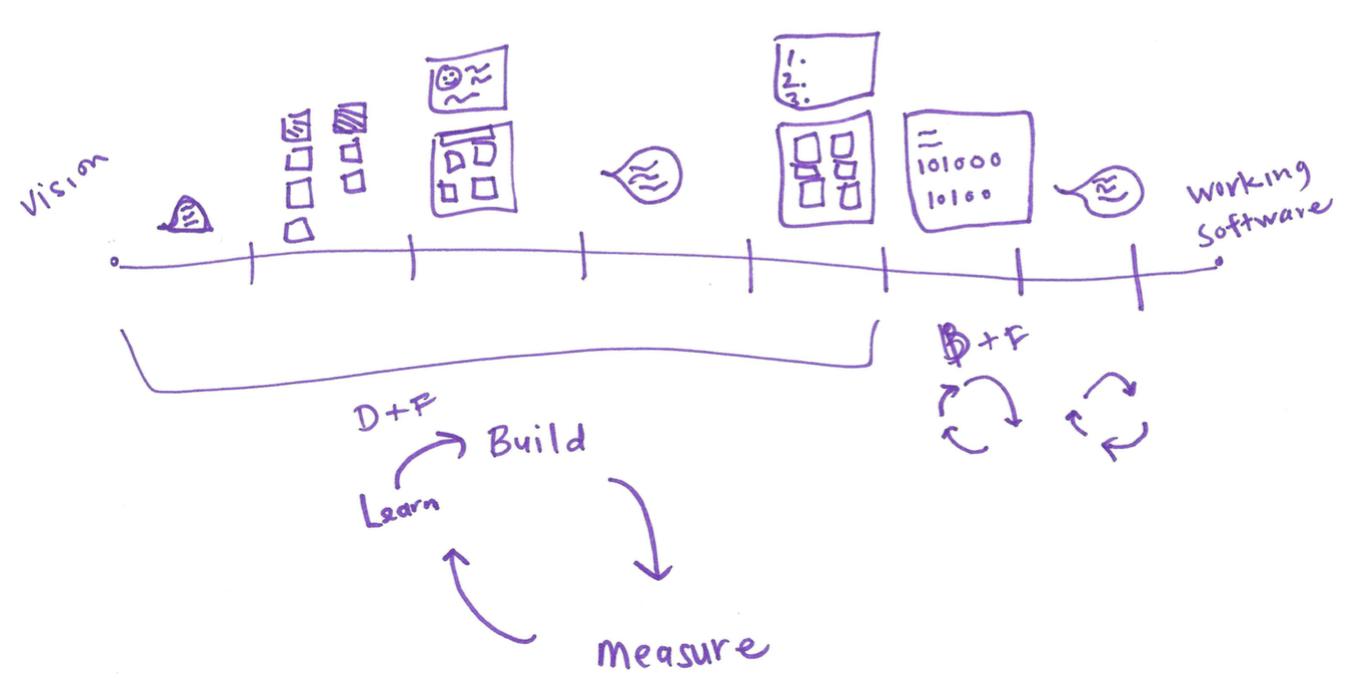
\includegraphics[width=6.5in]{interviews/2015_08_12_pm.png}
\caption{\quotes{2015-08-12 Product Manager's drawing of software development process}}
\label{2015_08_12_pm}
\end{figure}


\textbf{Todd:} If you're open to it, could you, on that sheet of paper, draw out how you view the way we build software? This is completely open-ended. There's no wrong answers. And just take a stab at it.  0:00:21

\textbf{Interviewee:} So I'm drawing a line, it's like product on a continuum. We're gonna have vision here. We're gonna have working. Can you tell I'm a PM coz I'm writing in lines, boxes can't do? 0:00:45

\textbf{Todd:} I love it.  0:00:46

\textbf{Interviewee:} So let's see here. So let's do a couple of lines here. Alright, so let's say, each of these represents two weeks.  So we'll say that the first point, so how we build it at pivotal is that what you asked?  0:01:17

\textbf{Todd:} Yes.  0:01:18

\textbf{Interviewee:} So it starts with having clients.  0:01:20

\textbf{Todd:} How would you build it too?  0:01:21

\textbf{Interviewee:} Yeah, yeah. Totally. The reason I asked about Pivotal is 'cause we're doing consulting. So if you're thinking of product as a continuum, our clients come in in all these different ways of where they the insert. But it starts with a conversation, kind of like a qualifying conversation of like, 'hey, what do you wanna build?', and like 'what's the fidelity of your idea?' And from there, we have a good understanding of if they're at a stage where they can build something, or if they maybe really need to think about it further.  But once we realize ok, they're ready for Pivotal , we'll start with a Discovery and Framing and not every project gets Discovery and Framings, but in the LA office, a lot of them do.  We're trying to get like most projects getting some a semblance of Discovery and Framing.   0:02:04

\textbf{Todd:} When would you not do one?  0:02:07

\textbf{Interviewee:} So we won't do one... I think we can make the case really for all projects could do with a little bit of DNF right? So even if you're like, I know where to build from. So with FYI rather, but for a PM, I'm thinking, okay my role is to help the client understand who are we building for and then what we are building and when? So for the, who are we building for, I think all clients.  It'd be great if we could do some user research with them even if they are like, we did all these user research just to do a quick gut check, like hey this makes sense, that'll be great.   0:02:42

\textbf{Interviewee:} But I think a lot of the times when we don't do them, it tends to be convincing the client or if there's a budget concern.  So they have enough of a fidelity of understanding who their target user is and who the secondary users are and have a persona and are focused on stuff like kinda key factors like, ok, if you're saying you want to build an app for the millennials and for college-age students and for the ages 25-35, that's pretty vague.  We do get that a lot, but we're saying, ‘ok, it's for millennials, so what gender are we going for?' Or is it, ‘what are their behaviors like?'  There's a lot of questions that we can ask on this conversation. and these qualifying calls to say, to kind of fish out, to think if they are ready to work with Pivotal, or if they have enough information for DNF or not. So, does that answer?  I guess that was a very specific answer.  0:03:44

\textbf{Todd:} That was great.  0:03:46

\textbf{Todd:} I interrupted your flow.  0:03:48

\textbf{Interviewee:} No, no, this is fine.  So I'm of the opinion that I would love it if we could have some sort of research with all of our clients and users. Typically when we do a DNF, Discovery and Framing, we do that for 4 weeks on average, sometimes it's up to 6 weeks depending on how many users they have and how many people they want us to focus on.  But we typically really try to work on 2 to 3 target users being 1 primary user and maybe 2 users of the system that kind of insert in their day.  And then we've done a 2 week of design first or Discovery and Framing but really it's just 'let's talk to some users and validate some ideas.' But the whole goal of this Discovery and Framing process is to do a couple of weeks of talking to users, of about 2 weeks and that's when we're doing some of those exploratory interviews, kinda turn it into elicit narratives to understand what their behaviors and what their days are like.   0:04:51

\textbf{Interviewee:} And then from there, we can isolate what are some of their pain points and what are some of the frictions and inefficiencies and how are they capturing data and what are the tools that they use and who are the people they're talking to.  From there, I guess one thing I didn't mention which is important is to say, what are the product goals that our clients have?  And what are some of the assumptions that they have about their products?  About their users where their products can help solve their needs.  We go into these user research thing like, alright, here are some assumptions, hypothesis that we have, let's test them. Out of that output of user research is that we have this, we do some synthesis and analysis of all of the things they're talking about.  We record the things that we saw, so if they're in a cubicle and they have tons of printed out papers because what they do is they get stuff by mail and then they have to scan it in.  Those are the things that we're seeing that are part of their day that can affect them.   0:05:54

\textbf{Interviewee:} What did we hear, like things that they're telling us about their day, and things like we felt that they're telling us. But maybe there are some subtext and some nuance there saying everything's great but their faces are really strained and you can tell they're really frustrated and their posture has changed when they're talking about certain subjects. Kind of taking all of the things that recording from our user sessions and then coding it by what we saw, what we heard, what we felt and then finding themes. What are users talking about? Usually when we do research, we try to do 3 to 5 users, so that way we have a good cross-sample and in case there's any extreme people that we meet, it kind of helps us give a better analysis, better data sample. So we'll kind of call all the information that we have and we'll go to them, too.  So we'll go to their cubicles or wherever their workspaces are. So we want to get a sense of their environment. Cause there's so much contextual information there that you can't get just from having a phone call with someone.  0:07:02

\textbf{Todd:} Yes.  0:07:03

\textbf{Interviewee:} So, then, that's usually about a couple of weeks doing some researching.  As we're doing the researching, we're capturing all of our information on notepads and then we're doing what we call infinity mapping, affinity mapping.  We'll get one of those big phone cork white boards and we'll take a listen to the recordings of when we're doing user research or if we can't record just looking at our notes ‘coz our notes are like, you're almost writing verbatim what people are saying.  Coz you don't want to put all your analysis in there at this point, you just want to get them to talk and get it all in, and then we'll take each kind of idea and we'll put it on a post-it note and we'll have a bunch of post-it notes around and they'll be coded by what we saw, what we heard, what we felt, and then we'll start seeing themes around this post-it notes.   0:07:54

\textbf{Interviewee:} So there's this one user that said there is a lot of things around education and tools and timeline and whatever it is.  Then we started noticing trends, so we'll start taking those nuggets and we put them across this themes and then we'll do that to all our users; and then from there, we'll do another round of synthesis and the ideas are going to keep condensing.  So then we have a synthesis of all the people we talk to and what the overlaps are and the themes of what their day is like, and the behaviors they drawn during that day.  And then after that, we'll map out their day, like what are the tasks that they're doing, and then map out from the tasks all those insights rather not insights but nuggets of what we heard from them, that we kind of collectively called down and condensed and we'll put those against the tasks.    0:08:43

\textbf{Interviewee:} So when they need to schedule a user for an event, these are all the things they said about it, or these are the things we saw and the things that we felt.  So then what's cool about that is we do that for every target user and you can map them out.  So you say 'here are three target users, here are their days and here are all the intersections of their days'.   So you can tell visually, 'oh, you know what, when this person does something, you notice the next thing, like, these two people are affected.' And then you can start isolating pain points and inefficiencies and you get these really nice overlay of what the system, not the digital system but just the users in the workplace and what their days look like.  So when I'm mapping out the process, I'm thinking of conversations, that's a little talk bubble.  0:09:43

\textbf{Todd:} Ok, I like it.  0:09:44

\textbf{Interviewee:} And then I'm having doing some synthesis. Someone do a little post-it map.  0:09:51

\textbf{Todd:} Ooh, I see the post-its.  0:09:53

\textbf{Interviewee:} There you go.  And then from that, we say, 'ok, based on our research, this is what we say a persona or what this user looks like.'  We think of 'what do they need? What are the tasks in their day and what do we need.'  So we pull out insights from that. Like, this user really has trouble communicating with the other people on this team because they don't have the right communication tools setup or whatever that is. They need a better communication system.  Once we have these needs, and bits and insights of who they are and what they need, then we can say, "all right, how can our products solve these needs?" So then we say, 'we have some product ideas based on what their needs are, let's validate them.'   0:10:55

\textbf{Interviewee:} Then we'll go back and talk to the users. We'll drop some wireframes and say, "all right, based on what you guys had said, we feel that here's a quick prototype, clickable prototype" And we'll use invision.  We'll say, "Why don't you click around? What do you think about these things?" we'll do some user testing there.  And then from that information, we'll further validate or dis-validate our product ideas and we'll do another product evolution but kind of the output of this 4 week on average DNF cycle as that you'll have Wireframes and then you'll have some personas. You'll know who your end user is.  You'll have empathy drawn for your end user which is the whole goal. You'll have a problem that's been framed and validated.   0:11:38

\textbf{Interviewee:} So that way, it really de-risks development cause it's pretty great to come in to development and we know that when we're making product decisions, we can go back to this research.  We're like, "oh, if we're going to do this or this, like, what do they actually need? Like what was that they talked about that really indicated this is the right approach?" It also helps us speak a language that our users speak.  Which is really important for the development team but all the other stakeholders involved in the process.  0:12:05

\textbf{Interviewee:} Words are everything, right? So we want people to be kind of on the same communication levels of talking how their users would talk, so that way it helps us draw all that empathy throughout the entire development process coz you still need to draw on that, you know 6 weeks, 3 months, however long into the development cycle until you're releasing. Right to be able to have that insight of what they want. I think the cycle is... Let's just say that you've done some analysis and you've done some wireframing, and then after that, we'll talk to users again.  After that, we'll do another set of wireframes. We'll also do some persona mapping here as well as making these wireframes.  And then after we do that, we will create a feature list.  0:13:13

\textbf{Todd:} Yes.  0:13:14

\textbf{Interviewee:} So, we'll say, like, we're not gonna…  Like, what could the next you know 2 to 3 kind of epic areas. We'll say, let's give some insights here.  Like, maybe, we have 3 insights and 3 needs.  Let's do 3 feature ideas and how do these feature ideas map these needs?  So we write these feature ideas and we'll say, down in the documents and user needs this and we'll help them achieve their goals.  Business needs this and this will help them achieve their goals.  We're always aligning user business needs throughout the entire process. So then when we get into development, we'll just make a little terminal, I wish I had multiple colors.  0:14:00

\textbf{Todd:} Next time, you'll have to bring your can.  0:14:03

\textbf{Interviewee:} So, when you're getting into the computer, when you're getting into development, you're able to have a backlog that's been built.  You have the first couple of weeks of features.   0:14:17

\textbf{Todd:} Yes.  0:14:18

\textbf{Interviewee:} You have some ideas and you start building and then once you release something, which could be in a week or could be a couple of weeks depending on what you're doing.  But once you get into the first bit of business value working software, then you can go and you could talk to your users again and then you learn from them and then you continue on.  So at that point, what you're doing is you're building something and then you're measuring it.    0:14:45

\textbf{Todd:} Yes.   0:14:46

\textbf{Interviewee:} And then you're learning from it right?   0:14:48

\textbf{Todd:} Uh-huh. Yes.  0:14:50

\textbf{Interviewee:} And then you're going back to building, right? So that's what we're doing for this whole process. So the feedback loop is really important.  I think, when I'm thinking about the extent, like the depth of all these research, you don't need to have a DNF to do any of these research, right?  You don't have to sell that in, you can do...  So the training that our designers and our PMs have, and now we're trying to have our developers be exposed to it, as well.  To say, ‘ok, developer, you get a client project. Development starts tomorrow, you can still talk to some users.  You can still setup user testing.'  And you can do that throughout the entire process.  So it's almost like this whole upfront part, with like the DNF.  You're making little DNFs through it, right?  So whoops, it's really you're taking this and you're kind of doing like DNF cycle.   0:15:42

\textbf{Todd:} Yeah.   0:15:43

\textbf{Interviewee:} Whoops, and you're doing that here, and then you're going to do it again. So, like each week, you might be bi-weekly.   And that is ideal, right?  But sometimes you don't get the users?  So there's a lot of, kind of…  You have to be pretty scrappy with how you do this sometimes, you don't just get this nice set of users at your disposal, you know; but it's so important and I think that's something we do a good job with is convincing our clients, like, we wanna de-risk this for you so this is how we can do it.  I mean go, it makes sense.  It's very practical stuff.  It's not rocket science honestly.   0:16:20

\textbf{Todd:} Now are you currently PMing a project?   0:16:24

\textbf{Interviewee:} I am.   0:16:25

\textbf{Todd:} I kinda noticed that every project, like, by its grain, is different.  I mean there's some commonalities but each one has its own, it's like children, each one has their own personalities   0:16:33

\textbf{Interviewee:} Oh, my gosh, yeah totally.   0:16:35

\textbf{Todd:} So, your current project, when you think of its uniqueness, what are the challenges or pain points that make this particular engagement interesting?   0:16:47

\textbf{Interviewee:} Sure, you know I think that, I think this is truly an opportunity and cool but it's a huge challenge.  We're working on a recommendations engine, and this recommendation engine, what does that even mean?  It's like pretty broad language and so we are, and you know, the term algorithm gets thrown around a lot.  It's like, what does algorithm mean.  And we also have some data scientist in the office, so when we talk about algorithms to them versus our clients, different connotations of the word.   0:17:21

\textbf{Todd:} They talk about the heuristics as well?   0:17:22

\textbf{Interviewee:} Yeah, they do actually, that would be more when we're talking to our data scientist coz our clients aren't quite to that level of knowledge.  But I think that's one of the challenges is making sure, you know, as PMs, that we're helping them deliver value, and they're not getting overly complex before they need to.  They say, they came to pivotal because they want to build this recommendations engine.  We're like "cool, but before you build this recommendations engine, you need an application that has a certain amount of data and functionality before you could recommend anything, you need people, you need conditions, you need affinities, you need restrictions,” or whatever it is.   0:18:05

\textbf{Interviewee:} So it's been our process to get them to, you know, and they've been really supportive of it, but they excited right?  So it's like managing their expectations throughout this whole process to be like, "don't worry we'll get to it, but we need to get to all these other things."  And what we get to, maybe, a little different than what you expect and maybe we don't get to it all, right?  So we're actually at the end of the engagement and we're trying some really cool things that are little less sophisticated than they expect but fully meets their needs plus more.  So I think that one of the challenges with this project is for them to say, "Hey, ultimately, does your end user, are they able to do the thing that they need using this recommendations?  And do these recommendations make sense to them?”  So, yes, cool, that's success to me.  They can schedule, so it's a scheduling app and then, and the goal is really to schedule these users to events.   0:19:04

\textbf{Todd:} Yes.   0:19:05

\textbf{Interviewee:} And then this recommendation engine to make it easier for the scheduler so they don't have to think about why they're scheduling people but they're like "oh, well i can schedule quickly coz I don't have all the burden of detail of why this person can go here and this person can't".  Coz it's very intensive type of scheduling that they're doing, that's all based on this…   0:19:24

\textbf{Todd:} A lot of constraints?   0:19:25

\textbf{Interviewee:} Yeah, well you know I won't even say it's a lot of constraints actually coz I think that actually one of the challenges is that I feel like we almost like spending a lot of time on the edge case right now, that the bulk of the app that don't necessarily need this.  There's a little bit of proximity and some stuff that makes it easier. So I would say that recommendations engine I say in air quotes like 101.  We hit and they can do pretty early on in this application but we some of the other stuff they're… they have, they just manually take this historical information that the schedulers has and just adapt it into the system or at the system; but then they also need to see how the schedulers use it before adding more complexities, right?  Because I think they have data in the system that they can add to this recommendations engine but we don't know if that is really what they need. We don't know what's the right data that they're looking for this?  So I think they want to put a lot of work into something they are not ready for, but we strike that balance.  0:20:29

\textbf{Todd:} So given the challenges and the uniqueness of this project, have you found yourself tethering or adjusting the way we work to achieve those goals?  0:20:42

\textbf{Interviewee:} I think that.  So, like, agile it's like a set of different tools, right? So I don't think there's one way to do any of the things that we're doing.  I think there's a baseline of process that we certainly need to adhere to.  Like we always have a planning meeting, we always have a retrospective, we always have a stand-up.  I think that's helpful for the communications side coz most problems are people problem, so it's nice to have a good strong communication system in terms of like tools that we use to do, to make product decisions, to develop wireframes.  0:21:20

\textbf{Todd:} Trying to do a...  Like you do have a baseline that we all use.  I'm trying to find the, what are the little recipes that you pull off to spice up the soup we're making.   0:21:32

\textbf{Interviewee:} Yeah, I'm sorry i already forgot what specifically you asked for that question?   0:21:37

\textbf{Todd:} Oh, I guess this is pretty open-ended but curious like as a PM, do you have these tools that you just like almost like playbook items that you could go and reach for?  I'm kind of curious in the particular project which things were you reaching for than maybe having reached for in other engagements.   0:21:56

\textbf{Interviewee:} Right, right.  I think for this one, so this one I actually came in toward the end of the engagement coz I was in a different project and I'm not fully working on this project.  So I have a couple of things I was billed for which is a very unique thing at Labs that doesn't typically happen. So I've been doing much more like enablement teaching on like how I make product decisions, how I cut down on really thick backlog.  I think for we're using data science, so that's something unique for this engagement.  We've been pairing with other data scientists and I've been doing a little more like kind of high level conversations, like really our engineers are working with data scientists.  But I haven't really done anything I think that's been super kind of unique that I wouldn't do in another project.   0:22:55

\textbf{Interviewee:} The recommendation stuff is different, I haven't worked on a project with recommendation stuff, so there is been a bit more like a designer who has worked on those projects a while ago set up this really nice like set of equations that have to do with decayed log and some other kind of basic loose algorithm need, just some equations for waiting.  So there's been some additional research I've done on recommendations and, like, kind of spending a little bit more time with the developers thinking through how we would do certain weighing and sorting but I wouldn't say that there's anything that has been so unique to this project that I haven't applied to another project.   0:23:34

\textbf{Todd:} When you described enablement teaching a moment ago, is that for the client's PM or who are you enabling?   0:23:41

\textbf{Interviewee:} Oh, the clients.  So the founder, the CEO is our PM for this project.  So I've been working with him just making sure that there's the basics of, this is how you build a story.  Like using that mnemonic of invest rate, like, it's the right size and the right value and have the right description and then there's, you know, kind of, worthy end of the engagement right now.  So you wanna do all these things and you think critical for your MVP and for going live is this, this and this. How can we think about search instead of having this isn't specific for this.  But an idea would be, like, instead of the doing a search function, which can be, like, take all the time that you give it, maybe to control F on the keyboard and then you can see, you could search that way.   So kind of trying to figure out some like ways where he can still get the value he needs, where he doesn't need to add so much complexity to it, you know.  Like he wants to do this kind of write up kind of HR function. I'm like, "well you have email right now", I'm kind of like, "how many write-ups doing per day?", like "can you capture this on Google drive spreadsheets right now and track the write ups for these people that way instead of putting in these functionality", you know,  0:24:58

\textbf{Todd:} Into the tool, right?   0:24:59

\textbf{Interviewee:} Into the tool.   0:25:00

\textbf{Todd:} Yeah, it's interesting coz the idea doesn't... I've worked with the founder on the recommendations engine with some graduate students and it's just interesting how I picture he had some…  He kind of want to think things will work in a certain way and wasn't always clear, like, if his solution would solve his problems.  And so I feel, like, as a pm, I kind of wondering if you were sort of massaging, make him to, like, re-think his solutions and then understand his problems first?   0:25:29

\textbf{Interviewee:} Every day.   0:25:30

\textbf{Todd:} Ok.   0:25:31

\textbf{Interviewee:} Oh, every conversation.   0:25:32

\textbf{Todd:} And how does that work and do you like facilitate that?   0:25:34

\textbf{Interviewee:} Well, I think a lot of it is I think about, like, ok, again this kind of goes back to like what are your business goals.  Like, you have a lot of business goals but what are your top 3 business goals? Who are your top 3 users and what are their needs?  So when you're making decisions and if it doesn't align with these, or if it kind of align with this, it's really easy to be like, well, this is your budget, this is how many hours you have left, what's more important?  Ultimately there are other ways of thinking about it. So there's a lot of, use some facilitation techniques like, I'm sure you've heard of like a Dump \& Sort or 2x2, right?   0:26:15

\textbf{Todd:}  Oh, 2x2 yup.   0:26:16

\textbf{Interviewee:} Yup. Yup. So there's things that, like, what you'll do when it really comes to \quotes{I wanna do everything.}  So there's a point in this project not so long ago where the development team didn't see eye to eye on this path because this path for now we kind of getting into the heavier recommendations stuff.  And there's a lot of opinions on how this should be done.  So we did a workshop where we did a couple of rounds of Dump \& Sort and 2x2s, so how we did it was there was purposely a break in between with lunch.  The idea was like alright the question I asked was, "what do you think the path is for what we're trying to achieve" or something like that.  It was more specific it was like, "what do you think we should be doing?", like, let's do a Dump \& Sort on that and so everyone did it and we have variety of ideas and we then we put it on a 2x2 on complexity and value I think, value on development of complexity in value.  0:27:17

\textbf{Interviewee:} So coz we're thinking like time, and then like impact. So we did that and we got everyone closer to the same page at the end of like everyone did agree that this is the first thing that we should be working on now and this is the second thing.  And then we said, \quotes{ok, cool,} knowing all that, what are some of the technical implementation details coming from that.  So we did Dump & Sort and that we prioritized again.  We didn't do a 2x2 at that point.  We just kind of prioritized some ideas, then we had lunch, we came back and I asked the same first question of, so what do you think this same path forward was?  0:27:51

\textbf{Interviewee:} And it was interesting because my hypothesis is that they'd be more aligned but they weren't. They actually were, they were closer but what happened was after we did that, it was just the Dump \& Sort, we didn't do another 2x2, but then we said, \quotes{ok, so what are, let's talk about this.} What came out of it really quickly, because we already framed all these conversation was this idea was like, "oh, what if we do it this way?', and someone was like, "oh, that's great." so everyone had consensus within maybe 15 minutes after we had this like round 2 of asking the same question, people looking like they were kind of divided.  I think it was because people felt heard that there is another opportunity to talk through some of their thinking, that they were more amenable to other ideas and we're able to get to that open creative space.  It was really cool, but I was not expecting that we'd come back and everyone would be like so diverse again in their thinking.  It's interesting, so I guess that was different.   0:28:51

\textbf{Todd:} What would you do with the client that refuses to prioritize?  They would refuse if you brought them down to the table and say, \quotes{let's do a Dump \& Sort}, and they say, \quotes{No, we won't do that. Everything is of equal priority.}   0:29:04

\textbf{Interviewee:} Oh, so I've done that a lot and I've never had someone say no.  I don't know.  We just keep working on it in different ways.  So I think like...   0:29:14

\textbf{Todd:} It all has to be done by this date.   0:29:16

\textbf{Interviewee:} You know the date-time too, that's definitely come up, but I've never had someone who's been that absolutely no, like, I won't play because there here to work with us and I think they understand they're spending quite a bit of money working with us; even the ones who might not have that true number in their head, they get that sense of "I'm here to make something work". I think that people come in here for the most part, I haven't witnessed people that have been so 'I'm closed off, I don't wanna do this'.  But again it's kind of contextual, so it's easy for me to create like scenarios or ideas once I know what the product is.  So I'll tend to say, ok, because there's a lot of, like, writer's block or prioritization block.  Part of our goal is to be facilitators and to pull out ideas and say, like, "ok, cool.  You want these 4 things to be done by this timeline, so let's just, lets' focus on one.  What do you think the number 1 is, let's start somewhere”.  And them like, "it's all equal”, but we'll say this", and then we're like, "ok, next one, is this one more important or less important than that one?", "Oh, it's just as important", and then alright, so let's dig into to it.  \quotes{So what makes this more important?  How does it achieve?} I might start writing "what are the goals of the product here?" and then "who are your users?" and then I can even say ok.  And then I'll prioritize that.  Like, some will have some ideas and stuff like "here's all the things that's important and we'll try to do some prioritization of product goals. We can usually get somewhere when we prioritize something and then I can match whatever it is that we're talking about against that.   0:30:57

\textbf{Todd:} Yeah.   0:30:58

\textbf{Interviewee:} It's, like, how does this help you get to your timeline faster, right? How does this get someone to do this easier?  Ok, cool, so is this to be more complex than that, so then maybe timeline's the big thing here.  Then let's go with the thing that seems least complex.  There's a lot of that, like, we're kind of totally use that, like, you know, time-quality-budget triangle, the project manager triangle you always hear about.   0:31:25

\textbf{Interviewee:} So there's a little bit of that, but we have fun with it, too.  Like I try to, you know, people come in here with so many different reasons and perspectives on what they're doing and why they're here and so I try to keep it as light as possible, too and try to really decouple the emotions and the behaviors and kind of lean on the process more.  So it's not, \quotes{oh, your guys}  fault that you're not agreeing.  It's the process, we need to be able to facilitate an environment where we can talk about our ideas and prioritize them together, right?  So we really try to lean on these consulting tools and process these and whatnot to make it a little bit easier for people to get their minds out.  And the Dump \& Sorts nice because it's a really cheap and easy way of getting people just to get their ideas out and in the beginning they might have nothing or they might have the first three ideas really fast and like oh now i have nothing. and so they will say, great whatever you want, like, maybe an earthquake can shut down your business or you know whatever the prompt is, like, we'll think of some absurd things.  Write bananas if you need to or whatever.  You know what I mean?   0:32:41

\textbf{Todd:} From your perspective what is the purpose, what is your goal of the IPM?   0:32:47

\textbf{Interviewee:} Oh, so I think the goal of the IPM is to say, \quotes{Alright, where have we been and where are we going?} So this last week, I always start with the… I guess it's about getting people on the same page and with understanding the same vision and understanding what the goals are of the product for the week ahead.  I think it's important to say "alright, here are the big things, here's how our environment has changed based on what we've deployed and you know here's currently what's being worked on today since waiting for this meeting.  Are there any questions about it?  Is there anything that we need to know that's being worked on now that might change these future stories?" and then we go into each individual story and we say, "Alright, here's our treasure map. Let's talk about some of the hidden complexity from this."  It's not about, in my perspective, to have developers write out every single tasks and implementation details but it's kind of that space to have enough of a conversations so that you can estimate complexity as a team for a specific feature story, and that you can leave that meeting having a good understanding of \quotes{hey, here's how the next two weeks look like knowing that things change.}   0:34:09

\textbf{Todd:} Nice.  So you spend some time at the beginning of the IPM reviewing what happened recently. And it's like that 5, 10 minutes?   0:34:19

\textbf{Interviewee:} Yeah, well, so let's say the IPM submit in like an hour, so the first I might say, like, "hey, I'll have tracker up."  And I'll say, "here are the largest things that we delivered last week, just as you're thinking about complexity, here are some of the things that you might we learned that this integration point is behaves differently than we thought, and we have some research that we need to do."  But it's like a minute to a couple of minutes, we don't spend a lot of time, it's like a very quick recap.   0:35:00

\textbf{Todd:} Yes.   0:35:01

\textbf{Interviewee:} And then we'll say, "Alright.  Here's a couple more minutes and let's talk about what we're doing right now.  So is there any question on the stories that you're working on? So here are the stories that are in flight."  The planning meeting tends to be Mondays so there's, you know, depending on your team size, but if you have 2 to 3 pairs or 1 to 3 pairs, there's only a couple of stories that are being start or that are started.   0:35:22

\textbf{Todd:} That's true. Right.   0:35:23

\textbf{Interviewee:} And we don't go through like, all 6 stories from last week or whatever. It's just kind of quick context coz it's Monday and people have a weekend, just want to remember what we're all working on.  But then my agenda as a PM is I want to have all the stories pointed with complexity and that there's conversations had to enough fidelity where people have an understanding of what's going on and that they also know who to ask.  And if there's any blockers or dependencies that I need to know about so I can start unblocking things.  So if you think about it, if you're doing, like, what is it, 2 weeks, 1 try to go over 2 weeks of work so the current iteration, the next and if you have (this is for non-engineers) say 10 stories, right?  So you're trying to get through a 10 stories in a week, that's pretty high but whatever.  And so have 20 stories that you need to get through, and you want to spend a couple of minutes on each story.  Let's say you do 3 minutes on each story, so that's a full hour.  It's all about saying that pre-IPM or just like, not even if you're having a pre-IPM but all that you need to so much research and like good work and write the right stories and that goes as soon as possible.   0:36:36

\textbf{Todd:} There's a lot of people in the room.   0:36:37

\textbf{Interviewee:} Yeah, there is a lot of people in the room.  So it's about finding your rhythm but I think the goal is to make sure that you have a brief overview and that you can tell if it's taking longer than that few minutes per story.  The story's not ready and you immediately got to pull it in and put it in the Icebox.  That's on the PM to really be true to themselves and make sure they have that the ability, it's part of their facilitation to be like, ok, I think there need to be discussion so let's pull it out.   0:37:06

\textbf{Todd:} Yes, interesting. I was on a project where I've realized that we didn't really have iterations.   0:37:15

\textbf{Interviewee:} Oh, interesting.   0:37:16

\textbf{Todd:} We were actually very present with the work, we would just show up and do whatever's next on the backlog and the purpose of the IPM was basically to make sure there's a pointed the stories in the backlog.  And then it was really interesting moment for me.  Coz there's other agile techniques where you actually agree upon what you're going to do with your iteration like scrum.   0:37:40

\textbf{Interviewee:} Yup.  Yeah sure.   0:37:41

\textbf{Todd:} Kent Beck's Extreme Programming actually says you should do that, that you should actually commit to the work you are doing that week and I find that at least the projects I've been on were much more present that if a PM in the middle of the week says we have to change what we're doing, we just do that.  We alter what we're doing, we're very flexible and so for us on my teams, it doesn't really matter what day of the week we do the IPM on.  Sometimes, we do that on a Wednesday.  It's just that when the client is available, it really tends not to matter. It's just interesting.   0:38:17

\textbf{Interviewee:} I agree with that.  Like, I don't think we have this kind of Monday, like start of the week with the IPM, Friday retro but let's say you're working on 1 week iterations and your releases on Tuesdays, then when does your week start then.  Maybe you have your retros on Monday and you do your IPM on a Wednesday or something like that, Tuesdays your retros, however.  I think the goal is to be flexible as you're saying. You know, I think, it's all about your team rhythm and what you guys agree upon as this is the process that works well for you.  So I do think it's nice to have this kind of like you know, XP or your agile, whatever your kind of flavor of process that you're using and then you can adapt to it wherever you need.  You know I think 1 thing we need to watch out for consulting is our clients have different levels of backgrounds in this work.  And so we want to teach them like a good base level process so that they could then figure out kind of what their version of it is, and then also, the kind of speaking to them, no idea of an iteration.   0:39:27

\textbf{Interviewee:} I'm on board with that but you don't want it to be too jarring for people so when you're pulling stories in and out of the backlog too much within a week, you just want to make sure you're not doing too much context switching and that you're not, that work you're doing or whatever planning meeting that you're doing, it's noted and that you're kind of bringing that into your week. I don't know, I'm with you; I think it's great when you would need to be flexible, I would like that, I would actually prefer that. I just worry about the clients and their ability to work in those kinds of such flexible environments you know.  I do like that we give them this kind of, for their first engagement, we also have clients that come back for lots of different engagements, I don't know. I like it, I think and I've had teams where we've just been able to move things in and out but it's also been that the developers feel like there's not much thrashing and they're ok with it. I think it's easier for PM to do that but harder for an engineer to do that.  I think there's so much more thought going into the tables that they're working on into how they're structuring the project. I think it can be done in the right way but I'm always really conscious of that.   0:40:43

\textbf{Todd:} I think the saving grace is engineers don't want to work on non-pointed of stories so there is a gating factor. i mean, if i just dropped in 10 stories at the top of the backlog and they're not pointed, someone in the team's gonna say "hey, wait a minute, we need an IPM."   0:41:01

\textbf{Interviewee:} Well, I think it's scaled to, right?  Like a couple stories versus 10 stories that's different thing but...   0:41:08

\textbf{Todd:} It's like if I'm turning a steering ship a lot, there's gonna be push back and say, "wait a minute, we need to talk about this stuff."  I'm just not gonna pick up, and if I slip one in then you know that's ok.   0:41:20

\textbf{Interviewee:} I think it's like what's reasonable for your group, too. Like if you're finding that you can develop deliver value and you're testing with user and you're not doing so much big change that like...  I think you'll have to have healthy user testing process if you're gonna do big change really quickly as well.  Coz if you do all these change and then you never check with users frequently, then how well do you know that the change you're doing is right? Coz you can build in all these different directions and I'm all about like I do side on small experiments that you're testing, so when you're doing really big experiments or just more risks with what you're doing.   So I guess that's more of in terms of the pointing, you can have developers point, you don't have to be in an IPM to point, I guess.  I think that's a misconception like you can have a developer pick up a story and point together or point with 2 pairs if you want that kind of...  But it also depends on what you're working on, on what you're pointing, like a text change versus like an integration addition.  Those are very different conversations, too; so I think it is really contextual. That's what I would say.  But the trashing is what I'm always worried about.   0:42:34

\textbf{Todd:} Yeah, yeah.  That'd not be good.  Thank you.  You've been very delightful.  I think we could go on forever but I think I can't. So thank you so much.   0:42:45

% \section{2016-01-08 Interaction Designer Interview}

\begin{figure}[h]
\centering
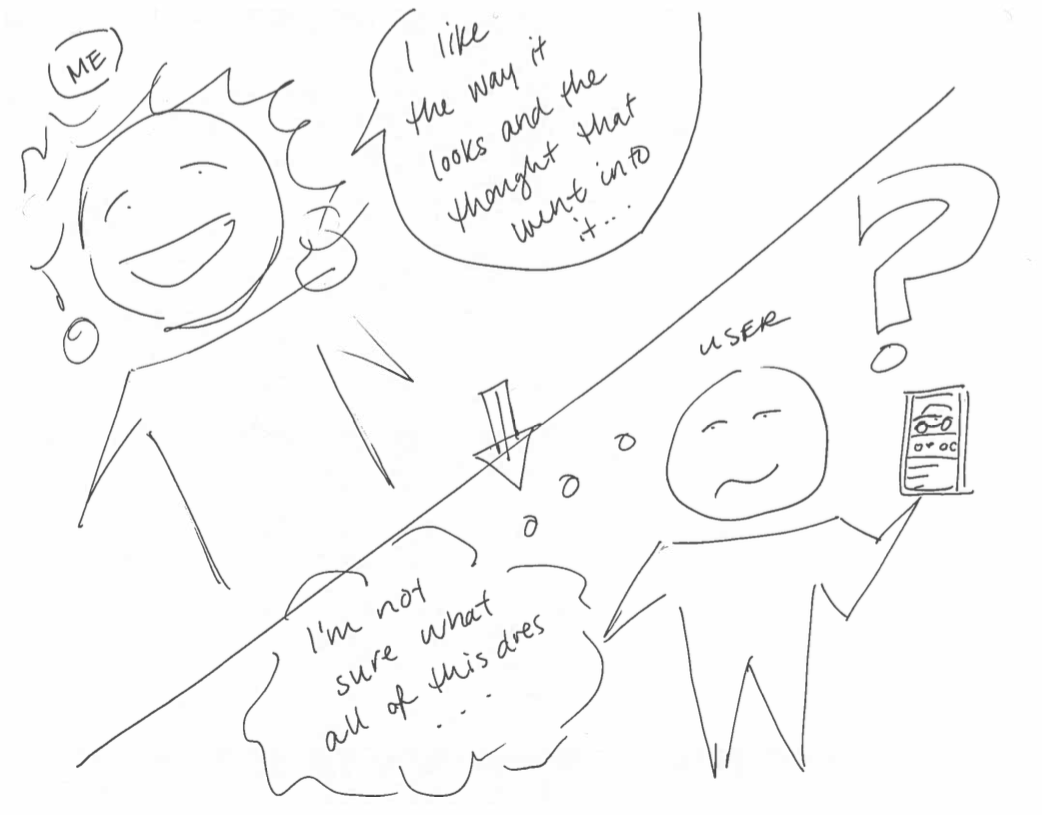
\includegraphics[width=6.5in]{interviews/2016_01_08.png}
\caption{\quotes{2016-01-08 Interaction Designer's drawing of software development process}}
\label{2016_01_08}
\end{figure}

\textbf{Todd:} My first question for you is very open ended.  00:02

\textbf{Interviewee:} Okay.  00:03

\textbf{Todd:} There is no wrong answer.  I was hoping if you could draw how you feel about the product.  00:09

\textbf{Interviewee:} Okay.  This may get elaborate.  00:27

\textbf{Todd:} Fantastic.  00:29

\textbf{Interviewee:} This is my new pen so.  [Pause] Here we are.  I did sort of a story board-ish type of thing.  02:54

\textbf{Todd:} I love it.  02:55

\textbf{Interviewee:} So, do you want me to explain it?  02:58

\textbf{Todd:} Please.  02:58

\textbf{Interviewee:} Okay.  On one hand superficially, I'm happy because aesthetically, I think it's nice.  I think it's, when you compare it to some of the projects we do, it's been going on for so long and there's such a huge team of smart people.  I feel like we got so much done and it's complex and interesting and there's lot of thought that went into it and it's a really robust app but I'm worried that even though it's pretty and we built a lot of features and the technology is cool, not all of it is necessarily useful for end users and I didn't even give the user name anything because I don't even know that we're designing for the right person all the time with some of our features .  I don't know.  So, I'm worried there were will be more confusion in the marketplace than I would like there to be in a product that I've worked on.  03:57

\textbf{Todd:} Anything else?  04:01

\textbf{Interviewee:} In the drawing or in general?  04:05

\textbf{Todd:} Both.  04:06

\textbf{Interviewee:} Not so much in the drawing.  I guess the big question mark is just that I don't know, I think it's pretty usable but I'm worried there's going to be features like predictive for the users or going to be like what is this or why do I care or they'll have question marks around there's something really obvious to me like \ldots I would like you heard a lot of feedback, I want a light telling me if my oil is low and that's just not something we could do because of constraints on the technology I think.  So, I'm worried if people will look at it and say why is there all this stuff that I don't want and there's some stuff that maybe feels really obvious to some users that we haven't provided for one reason or another but overall, I still feel happy.  I think we created a solid product.  04:59

\textbf{Todd:} Good.  When you were describing your \quotes{you} picture, you used the word superficially.  I don't remember the exact word but something like given this superficially I feel happy about it and I was curious if there was like an under feeling of the product.  05:17

\textbf{Interviewee:} Yeah, currently to some degree, this is the under feeling.  The superficial part is a little bit as a designer is a normal person walking around, you feel like people look at it and like it's so beautiful and that might be the beginning and the end of what they think of the app.  They might not use it.  Maybe, it's not for them.  I feel like I could put it in a portfolio or take some of those App Store screens and show it to people and maybe like oh my God, this is the nicest product, you must have done a great job or your team must have worked really hard but if we built something that's really beautiful but doesn't meet the needs of our users, it's kind of I'm still superficial.  I guess part of me is still happy it's beautiful at least or that there's parts of it that are really pretty but at the end of the day as a designer, it's kind of a big fail to build something that's pretty but not the right thing.  It should be a big fail for everybody but especially as the designer, that's what you want to avoid.  06:21

\textbf{Todd:} Yeah.  So, what do you do with that tension?  06:25

\textbf{Interviewee:} During the life cycle of a product, one of the things we enable people on or if you work some more even not as a consultant, I feel like a part of your job as a designer is to constantly be educating everyone else that things that look pretty but don't work are bad designs.  I think design isn't about just making it pretty.  It's really more about making it useful.  And so, that's something that I think is a big part of our design enablement here that we work on consistently now that I'm rolling off the project.  It kind of is what it is.  I guess if I was staying on the project longer, I would keep pushing and I think the design team as a whole would keep pushing back on features that we don't think meet our user's needs and keep pushing for features that we think might not be as popular from a business perspective but would be popular with Hannah and Michael.  07:35

\textbf{Todd:} How does this affect \ldots well this is your last day.  How has this affected your motivation for the product or for the project?  07:44

\textbf{Interviewee:} Not negatively.  This is \ldots I guess I'm happy face because even though I have some question marks about some of the features, we had to prioritize and how you solve that.  There's still things we fought for that weren't on our original feature list and actually got to put in.  We did research and we know these features are going to be popular with our users and that's a huge win and also happy because I'd rather make something that looks polished or looks good even if it's not perfect functionality than something that doesn't have all perfect functionality and looks bad.  So at least if it's beautiful or elegant or it feels sexy to some users that's still your part way there.  It's just not the whole picture.  08:39

\textbf{Todd:} Cool.  So, it sounds like your motivation is either intrinsic or extrinsic.  It's outside of like I don't know is it the product set or the features or the \ldots I'm trying to ask.  Yeah, I guess what motivates you when you think about you as a designer.  08:59

\textbf{Interviewee:} I think it's more intrinsic which is why I'm happier being a designer than some of my past jobs and I think part of it is the process of building something or making something.  I really enjoy that starting with nothing and you know at the end, there's something out there that wasn't there before.  I find that kind of creative, creating and build process really satisfying.  I like the problem solving.  I think I'm motivated to solve the problems as creatively as possible or get a team to do that.  09:49

I like making things better so it's \ldots to some degree, joining a project that's a mess is hard or joining a project where people are unhappy or you know going in, it's going to be difficult.  It's hard at the same time that's where the interesting stuff is if you join a project and it's super easy and there's low expectations.  It's just not that satisfying for me because I'm not making that impact.  So I guess partly, impacting either the team around me or the product itself and the end users.  Those are probably my three things when I feel like I'm impacting all of those then I'm probably pretty motivated.  10:35

\textbf{Todd:} The team, the product and the users?  10:36

\textbf{Interviewee:} Mm-hmm.  10:37

\textbf{Todd:} Okay.  And you were describing projects that like people were unhappy or there's a mess.  Did you feel like any of that was true for this project?  10:47

\textbf{Interviewee:} The unhappiness, yeah.  10:49

\textbf{Todd:} Okay.  10:50

\textbf{Interviewee:} People have been more vocal or either people are less happy or they're more vocal about their unhappiness on this project perhaps just because it's longer and it's little different and I felt more of that coming from frankly San Francisco and I think it's because they're more process oriented.  When I worked there, it felt like they're very rigid on process and here, it's more flexible.  So, I think there just seems to be more people on this project who are feeling maybe burned out or upset about stretching or changing our process to fit Oscar.  11:34

\textbf{Todd:} Can you think of an example of where we were more flexible with our process or something we changed up maybe \ldots yeah, can you think of an example?  11:49

\textbf{Interviewee:} I mean from a design perspective, I do feel like this project more than others I've worked on here, we've had to compromise on prioritization so we're prioritizing not, it's not user-centered or design feels less user-centered than average and more business goal-centered.  So, I think there's been some tension in design around having to prioritize things that we know people don't want either are neutral or net negative for people that are going to upset users for the most part and we have to do it anyways just because there's a business reason .  And being far away from the business probably doesn't help either because instead of being able to have that one on one conversation with the decision maker, I feel like we're hearing through layers of people and so you don't feel totally heard all the time but I also know that a lot of the devs are very sensitive to that too.  I think perception-wise, it's so hard to build things.  No one wants to build something and spend all that time coding something that doesn't matter.  13:05

\textbf{Todd:} Yeah.  13:06

\textbf{Interviewee:} So, I know like when we did inception, there's a lot of questions from the dev team about things that weren't user-focused and I definitely have people commenting after, to me personally, or I overheard conversations about why we are doing this if it's not important basically or that business reason doesn't feel important to us.  13:34

\textbf{Todd:} So although the client was very focused or in part to say prioritizing around their business needs, I saw us doing a lot of user interviews so should I be surprised by that or how do I reconcile that?  13:54

\textbf{Interviewee:} So, that's a really good question and I had a conversation about this yesterday.  So, I think there's a couple gaps \ldots so partly I think it's great that they bought into that process.  Someone somewhere was ok paying that and letting us do that and that some level of buy in, that's more than maybe they had before so that's awesome.  Just because we're doing it though doesn't mean the results are being followed or respected so I do feel like we did a lot of research and then came to conclusions and people said yes, that's great, now we know that about Hannah or we know that about Michael and then things still weren't prioritized according to that.  14:44

So, you can research all you want but if the priorities don't follow the research then you're not totally buying into the process I guess.  I'd be curious to see some of the justifications where we're just not prioritizing it now.  We have those research findings, we know this about users but we're pushing back, we'll do that in a month or the next month or the next release and I think sometimes that can be really valid.  You have to prioritize and sometimes, it's not always what design wants or what a particular user wants but I hope it's not being thrown away entirely and we don't know.  15:25

\textbf{Todd:} Yeah.  15:25

\textbf{Interviewee:} The other interesting thing with research here was that while our clients were happy to let us do as much research as we could coordinate on our end, those weren't really are users.  So, the people we talked to here were American versions of Hannah and Michael but that's not actually who we're building for.  So earlier on in the process, I think there was research and we got good feedback that American Michael and German Michael were about the same, there's a lot of overlap but I think Hannah is a persona that's going to be further from a German Hannah so American Hannah and German Hannah might have a lot less overlap.  16:13

So, I am concerned that there wasn't any buy in for doing research in Germany and we asked a lot to get people to find a friend, ask a family member, email the guy that sat next to you before you came here and we couldn't get anyone to come up with even one which is a pretty sad number.  So, I think there's sort of like an outward buy in to the research but there wasn't a full buy in to the importance of the research.  16:46

\textbf{Todd:} I'd been looking at this.  So as a developer, there's a bunch of us writing code.  On iOS, there's 10-ish that's writing code in one codebase and there's this interesting tension between this idea of ownership and like \quotes{I made itπ} versus \quotes{we made it} and by looking at that dynamic and I was wondering for you as a designer, there is obviously a lot less designers working on the product, what does that look like for you?  17:16

\textbf{Interviewee:} I think it's the same type of tension.  It's really different at Pivotal which is one of the reasons I wanted to come here.  I think on my first day, I was in a kick off for a brand new project and Janice was facilitating and people were, some of our clients were asking about that some sort of proprietary and kind of around just how we do things and she said you have to be a grown up to work here, you have to be a real grown up , you have to be really, really adult to just kind of let go of a lot of the more petty things that people get hung up on in other workplaces that are okay and that just won't fly here basically.  18:01

And one of the things for me is that ego of that's my design.  I think that's super popular or super common with designers and it's sort of encouraged with talking about people like Johnny Ive who like is inventing everything at Apple.  Those are not all his designs but if you think of Apple and you think of him and people think he's kind of this God that designs all the things.  And I think some designers really, really love that the whole \quotes{that's my thingπ} and I'm not open to a ton of I do design critics but I don't really want to change my designs or I'm fine changing it but I don't want other people changing it, I don't necessarily want feedback from devs and people are kind of hung up on that.  18:46

And there's just not very much room to do that here which I think is great because it makes you, you kind of have to just if it's very Buddhist like you have to let go.  You just put it out there and then it's its own thing and you don't get to own it and it's not about who had the idea or I'm doing this and it's my baby.   You just completely have to sort of release the designs into the wild and expect it to not be yours.  And I think that's really good for me personally.  19:23

\textbf{Todd:} Why so?  19:25

\textbf{Interviewee:} Because I think it forces me to think about what's best for the product and really get in that mind-set of what's best for the team and not what's best for my special baby, this one product or this one part of the product.  And the more the larger project is, the more important that is because then you start getting like in my last company, we were building a suite of apps.  Each app had its product owner or product manager and those product managers would fight ruthlessly for resources and attention and designers and developers and things like that and it cannibalized the business vision as a whole.  So, one app was getting way more resources because their PM fought more effectively for it and other apps weren't and those other apps were just as important to kind of building a platform.  20:21

And I see it a lot even within one product if it's chunked into pages, if one product gets all the love or has a more experienced designer devs that are better with what they're doing on it and others are left to kind of languish.  It feels unbalanced within the product when everyone should be sort of working towards we want the best possible product that's best for users, it doesn't matter if I made the design or Karina made the design, I started it and she picked it up.  We just want the best thing out there.  21:01

\textbf{Todd:} Cool.  So, I think I've got it in my words hearing you've transitioned from like \quotes{I made this} to \quotes{we made this} and is that true?  21:12

\textbf{Interviewee:} Mm-hmm.  21:13

\textbf{Todd:} And I was curious from your perspective, what things enhanced or detracted from the \quotes{we made this} like what things would \ldots have you noticed that or you feel pretty bought in with the \quotes{we made this} like you feel like yes, we did make this?  21:31

\textbf{Interviewee:} There's this special magical balance that's hard to find and I don't think you can predefine it of you don't want it to be all about this my design, the designer owning it or the devs owning it but there's definitely you can swing the other way with too many cooks in the kitchen or no one taking ownership and no one feeling bought in enough to turn down and I'm having this decision or making it, someone has to make a decision and be the voice of the product if you're doing balance team or the voice of the user. And sometimes, I think we skewed towards the end of \ldots we spent too much time discussing or being sensitive with each other's designs and not just saying, okay well even though this is my idea, I still think it's best and promoting ourselves in saying my idea is great, let's go with it or I know you have all these other ideas but I think none of them are in service to the users as much as what we've got so let's not do that.  22:31

Sometimes, I think we end up being too sensitive especially the larger the team gets because we want everyone to feel included and to feel ownership but then it's like doing things by committee  then maybe the product isn't as strong or nothing, things aren't getting done as quickly.  So to be specific, we started feeling that as a design team when we had four of us working, we really liked to having, there were times when having two pairs being able to work independently was great but when all four of us sometimes kind of coalesced in one thing sometimes it was great and we had a really unexpected new idea that made the clients happy and made our users happy but other times, we felt like it was just too many people like decisions weren't being made, yeah.  23:35

\textbf{Todd:} One of the things that developers struggle with is well, we like this idea of constantly improving the codebase and with a large team, it can happen that you might say, \quotes{Oh this thing here needs improving, someone else will do it} and if everyone is doing that then nothing's going to improve.  I was curious if there was a corollary to that with design?  23:53

\textbf{Interviewee:} It's like design refactoring.  23:55

\textbf{Todd:} Yeah, I mean are there things where you're kind of purposefully make sure that the forest is cleaner at the end of the day then at the beginning?  24:03

\textbf{Interviewee:} Honestly, I feel like if you're thinking of it as like what's the grunt work that most people wish they could avoid, it's more things like we're doing now like at the end, we're doing a lot of dev support which I think everyone here loves working with devs and dev pairing but things like language support where you're like oh, I had this great design, we'd all agreed, it works and now we keep putting it into like 15 new languages and then tweaking and having to kind of solve these hard problems that are ill defined and really, really tiny.  For me, that's what I would prefer to avoid or like tracker clean up, things like that.  24:46

Occasionally, we have our InVision prototypes and at the end, it would be great if we could carve out time now to say okay let's do a prototype clean up to make sure that there is nothing in there that shouldn't be, we have every single screen we need there and it's just all clean and all the links are working.  Probably, we don't really want to do that and it might not get done.  So, there is a little bit of clean up but I think it's even less defined than refactoring for devs so.  25:24

\textbf{Todd:} We have this idea of making our tools better.  Do you have that same idea too like taking time to \ldots? 25:54

\textbf{Interviewee:} I think designers especially enthusiastic ones \ldots well designers tend to fall into two camps.  A lot of the designers around here like every time there's a new tool, we don't make our own tools as much I think as devs so every time there is a new tool, people want to test it out and sometimes it's great like \quotes{Hey, there's a thing called Sketch, let's try that} instead of using Photoshop and Illustrator which was the best thing that's happened ever.  26:01

Other times I mean since I've been in Palo Alto, there's probably been at least 10 Slack channel discussions about a new prototyping tool that people are trying and then it isn't really different or useful or worth the time of exploring.  So, you have to find that balance.  If you want to stay current, you would definitely want to update to a new tool.  If it's going to be a time saver, you're going to love it more if it works, if it's going to be better for the team but I don't think we should be trying every new tool or spending more time on updating tools and we aren't actually designing and doing dev support.  26:43

\textbf{Todd:} You were discussing a while earlier about not feeling heard by the client and I wanted to briefly explore how that affects your sense of \quotes{we built this} or your sense of ownership.  Are they related or they're not related?  27:01

\textbf{Interviewee:} Yeah, I guess in a couple of ways to one degree.  Sometimes, I've catch myself thinking I'm glad this isn't just my design because if I was the only designer and people were kind of like Andrea is the designer for this product and the product is out in the marketplace and there were a bunch of features in it that I didn't want in it that business is prioritizing and everyone looks at it as \quotes{Ooh, what designer okayed that.}  I kind of would have this inner dialogue with myself about \quotes{Oh my God are people judging me} because I designed really spammy right aloud in the product, these really spammy notifications and some that like anybody could look at and assume would probably annoy lots of people but at least on a larger product when there's many designers, I don't feel as much ownership, I don't feel as much stressed about business decision or product decisions or other designer decisions that I really disagree with.  28:12

It's kind of like well, it's not my baby, you can't win every battle and trying to be a good teammate and compromise and we have to be okay with some of the business decisions especially because I don't know everything about the business.  They could be amazingly valid business decisions and that's not my role in this project to question them or even know all about them.  So, there's things that don't might even feel wrong to me but again, it's not just my thing, I'm not the user and I'm not the only designer so it might be really right for reasons I just don't know about.  28:50

\textbf{Todd:} For us as programmers, we have this interesting schism between the code and the product and it's possible if you're really excited about the product but the code is a mess.  It's also likewise easy for us to feel great about the code but the product is a mess.  Do you see that happening?  I was just wondering if you like is \ldots well, I was hoping you would answer that question.  29:20

\textbf{Interviewee:} I think it gets back to this.  This is the most common one I see in design that I feel of \ldots 29:28

\textbf{Todd:} It's pretty but no one wants to use it.  29:31

\textbf{Interviewee:} And people get really upset and the Dribbblification of design of this, hey as long as it's beautiful or let's just copy someone else's beautiful thing without their being fought behind it or like just because it's beautiful, someone else makes something beautiful and functional and you copy the beauty and you use the same exact colors and fonts and everything make it look really slick but like maybe that doesn't work for your product or that's just copying, it's cheating.  So, I think that's the schism for us as you can look at something and appreciate the visual design but you can't even always assess I guess the user's experience or the interaction design.  Sometimes, you can but unless you know the users.  If I'm not even the intended user, it's maybe in another language.  I would never understand that market space.  I mean it's an enterprise product.  I can't really even assess if it's good or not.  It's not my business to but everyone can look at something the design and say, it's pretty.  30:41

\textbf{Todd:} So in your mind, there's this like there's the UX, how the features are used and then there's the painting, the design, the glossy looks.  30:53

\textbf{Interviewee:} There's overlap.  There's definitely an intersection and probably like with developers if the code is really great and maybe more likely to have a product that you're also very proud of, if your code is absolutely a mess it's hard to have a product that's not buggy which might bring a lot of people to, might make you feel worse about your product.  31:13

\textbf{Todd:} Yeah.  31:13

\textbf{Interviewee:} So for designers, looking pretty is part of it.  It's just sort of maybe your product version of, people can't see the code underneath so you can have code that's a mess and as long as the product is great you could say, \quotes{Hey, we're proud of the product, we just know we need to refactor.}  If it's beautiful, a lot of people look at the product and say, \quotes{Oh it's beautiful, it must be great} or they're willing to try it in a way that maybe they're not if it's not beautiful but the interaction and how users actually work with your product is a little more hidden so sometimes that's the part that beautiful product, you may just assume is good and it's not.  Alternately, you can have a phenomenal product that is simple and works for users and meets their needs really well and it's ugly and that can be okay too and people can be okay with it.  There's a lot, Google like Gmail.  32:11

\textbf{Todd:} Yeah.  32:11

\textbf{Interviewee:} Not beautiful but do most people use it and totally appreciate it?  Yes, it can be a great product and not have like a fantastic visual.  32:22

\textbf{Todd:} I was thinking about your workflow, roughly the features, the personas and the features and the filling in apps and then the sketching and like you test that and you have the concrete mocks and then a bunch of engineers actually implement it.  Does your sense of ownership like transfer at each stage or there could be gaps like I don't \ldots are there different sense of it like that's more real or I'm more invested in?  32:57

\textbf{Interviewee:} Yeah, and I don't know if most designers would feel this way or if it's really just very personal but for me, I'd feel more ownership over like wireframes and visual design because it's I think a lot more tangible and then I feel more ownership weirdly over the UI which I don't even build but I feel more empowered like the UI reflects more on me so like I'm excited to do design dev pairing because that's what I want to be adjusting pixels or I want to be making sure that the color that's being displayed is the color that we intended and if it's not, what do we do.  33:37

The research part for me, I feel less ownership over that and I don't even really know why.  I think it's just less visual and tangible like it's insights but then the whole goal is to share those and it's often a group in a room and they're not my insights, it's stuff I'm picking out of someone else's brain so I feel less ownership over the research process and even the insights than I would over the wireframes and the visual.  34:13

\textbf{Todd:} You mentioned you feel a lot of ownership of the product, the UI that the developers build.  Do you feel any ownership of the code?  34:18

\textbf{Interviewee:} No.  34:21

\textbf{Todd:} Yeah.  34:22

\textbf{Interviewee:} Not unless I've helped code.  So, I can code so when I do then I feel ownership of it.  If I built the website and it's in the code.  34:33

\textbf{Todd:} I made that css.  34:34

\textbf{Interviewee:} Yeah.  34:36

\textbf{Todd:} Okay.  How about our process?  Do you feel ownership over the way we do software development here?  34:44

\textbf{Interviewee:} I wouldn't say ownership.  I think I'm more focused on mastery or levels of understanding of the process so in facilitation of the process or enablement of it.  I don't feel that it's mine I guess.  I didn't invent it and I'm really conscious of that fact .  I think like Janice invented some things that I do or whoever came up with XP inventing, came up with the concepts that person feels like the owner to me.  I feel like I'm practitioner and I think more about like how well am I practicing somebody else's process or how long I'm like embodying the Pivotal process, how much do I agree with somebody else's process not so much ownership.  35:38

\textbf{Todd:} Do you feel empowered to change it or do you change it?  35:41

\textbf{Interviewee:} I do but I feel like I need to maser stuff before.  It's sort of like learn it and then feel free to break it.  You learn to do it the right way and then you can break it as much as you want and it's okay but I'm starting \ldots I'm just, I feel like the last couple of months, I started feeling comfortable with the idea that I want to create some of my own concepts or processes and that's okay and that's stuff that I'm starting to be comfortable teaching to other people too.  It's like if I see something enough and I believe it, I'm going to start doing it and if it works, it's okay for me to start talking about it as if it's a real thing, yeah.  36:24

\textbf{Todd:} Cool.  We've talked about a lot of different concepts here.  Tell me one more thing if there's anything percolating in there.  I'd love to hear it.  36:42

\textbf{Interviewee:} I guess I always wonder about \ldots I mean we should, I should go talk someone.  It is weird to me that I feel a lot of ownership over the end product and over the UI of it almost but no ownership of the code and to some degree, I feel like I have a super easy job because I don't build anything like I get to do some of the fun stuff.  I think about it a lot, it creates some plans like being an architect but I'm not the general contractor and I'm not a builder.  I don't really execute.  I'm just sort of on the team and I wonder \ldots I'd spent a lot of time wondering how engineers feel about that and it seems different between different people and different companies but sometimes I'm like how do engineers feel I here about designers and is that annoying to get designs then have to, do you feel like you just have to execute on someone else's ideas, are there people feeling really relieved like \quotes{thank God, I don't have to do this myself} because it's really boring or difficult.   37:52

\textbf{Todd:} Interesting.  37:54

\textbf{Interviewee:} Yeah, so I feel like there should be tension there because I feel like I got the cool job.  37:59

\textbf{Todd:} You think there should be tension between engineers and design?  38:03

\textbf{Interviewee:} I'm surprised there isn't more I guess.  38:05

\textbf{Todd:} Yeah.  38:05

\textbf{Interviewee:} I don't feel like I've felt it here in Palo Alto very much at all.  I felt it in some other jobs or companies with individuals who like to design and code and sort of and especially past jobs where everyone had more ownership over their domain, it felt more like hey you're stepping on my toes if you're trying to design and code but I'm \ldots 38:32

\textbf{Todd:} Can I answer your question from my perspective?  38:34

\textbf{Interviewee:} Okay.  38:34

\textbf{Todd:} If that's helpful.  38:35

\textbf{Interviewee:} Yeah.  38:35

\textbf{Todd:} So, I don't work a lot with you.  My first designer was Aaron, I worked a ton with and what I really appreciate about Aaron is \ldots so when I see that conflict is mostly like designer saying this is exactly what you have to build and that thing should be three pixels to the right and it's very like it's legalistic kind of perfectionism approach and Aaron had a refreshing sort of this is his style just openness and just saying \quotes{Hey, if this is not working, I want you to help me} like he viewed that the developers is almost as first line of users and having him actively listen to our input saying like Aaron we're building this and we don't think this is going to work like the UX here is not working for us and we think these are the issues and he will listen to that.  39:29

And so, that made it like really fun to work with him because it felt like there was a space that we both got to play in.  So, I don't know how every developer feels it.  For us, there's so much creativity in the code that I think losing the creativity in the mock ups is fine and I still found Aaron, a lot of the designers very open to like \quotes{Hey, I don't think that's the right font here} like I can't see those or that \quotes{Man, that really looks really close in the edge, should we add some padding} so even though I don't have a design training like showing it with some design ideas was often welcomed.  40:06

\textbf{Interviewee:} Okay.  40:07

\textbf{Todd:} As oppose to like \quotes{Oh no, this is my design, you can't change it.}  So, I think perhaps the fact that there's flexibility with the designers in the way that you build your designers and it's more of the \quotes{we} as oppose as \quotes{I built this} enables the developers to enter into the \quotes{we.}  40:23

\textbf{Interviewee:} Yeah.  40:23

\textbf{Todd:} In a way that's healthy.  40:26

\textbf{Interviewee:} And I think partly that's why there seems to be less tension here with that because we don't have that, no one has that ownership.  So, people are a lot more flexible all across the board with the changing things or accepting feedback or collaborating .  40:41

\textbf{Todd:} And then on websites, Aaron didn't know much about like CSS encoding so often, we would put him down on the IDE and he could like up and down it like Chrome whereas Richard will get in there and start messing with the CSS and so, those are kind of cool to see that like difference.  In iOS, I think it's harder for designers to come in and like it's harder for us to tweak things.  41:05

\textbf{Interviewee:} Yeah.  41:05

\textbf{Todd:} So, it's hard for me to draw conclusions from this project.  Is that helpful?  41:13

\textbf{Interviewee:} Yeah.  41:13

\textbf{Todd:} Okay.  41:14

\textbf{Interviewee:} Yeah, I think everyone is different.  I just always wonder, yeah, I don't know.  Sometimes, there's tensions and sometimes there's not and I just wonder like \ldots 41:30

\textbf{Todd:} Do you felt tension here at Pivotal?  41:32

\textbf{Interviewee:} There was some of my first projects but it was more I think the devs, it was my first, it was first project at Pivotal for me and I was the only designer and we had three PMs and that was kind of a mess and the PM that was turning, was supposed to be the full-time long term one was brand new also and then we had very experienced devs.  And so, I kept wanting feedback from him, I wanted help and I'm not.  I hadn't \ldots I'd been a non-visual designers so at my last jobs, they were very silo visual and interaction were separate so it's my first job where I was also responsible for the visual design and I really wanted that input of you're screwing up or this isn't a Pivotal way of doing things or hey, we think this would look better like this and I kept asking and they weren't giving it but then sometimes they joke about it after the fact that's like you could have just told me, I really did want you to tell me if there was 30 shades of grey, why didn't you stop me at 15.  42:42

\textbf{Todd:} Yeah.  42:44

\textbf{Interviewee:} So, there was kind of some emerging especially visual design where I was like I wish you got, you didn't to worry about stepping on my toes, I really wanted you to come voiced concerns earlier and not wait till there was dev design pairing or clean up at the end.  43:00

\textbf{Todd:} Yeah.  43:00

\textbf{Interviewee:} But I think they just didn't feel as empowered to do that like I would freak out if they did and then we got another dev who just loved front end and he was basically like I'm going to tell you if I don't like something and we're really open about it and then that was great and we didn't always agree and sometimes, we'd have to compromise or one of us will win but he was really upfront and that he would become kind of the bridge in the project to just giving really honest criticism of what was going on.  43:33

And then we had another developer who was rolled on that was really interested in research and she became sort of the bridge between design and dev just in terms of why we are doing and so she communicated a lot like hey, why are we doing what we are doing or this is why we've prioritized but not since then.  It's the only the project where it weirdly even though it was in a huge team, it did feel more siloed and partly I think that San Francisco like people are more was very like that's the process, I'm not going to \ldots44:08

\textbf{Todd:} Interesting.  44:10

\textbf{Interviewee:} So, I just felt \ldots I don't know.  I haven't felt since then like there needed to be a bridge because it's felt more like collaborative and whole team focused so I love it more or less like we needed a rep and that person was going to communicate to this people and \ldots  44:27

\textbf{Todd:} Wow.  44:27

\textbf{Interviewee:} Yeah.  44:28

\textbf{Todd:} I have appreciated Richard just asking occasionally hey what do you think of this or I've got these two things or I got these six things which ones and like that sort of pulling.  I felt like that was fun and it's nice to be involved.  It's always nice if someone asked you for your opinion and I appreciated that.  Cool.  Anything else about the topic of ownership or yeah?  44:59

\textbf{Interviewee:} I don't think so.  45:04

\textbf{Todd:} Do you have any feedback for me as an interviewer?  45:07

\textbf{Interviewee:} Here's one.  You could try and I've tried this and I don't know how successful it is but I would love if you try it and let me know; doing like mirroring of posture and stuff.  45:31

\textbf{Todd:} Okay.  45:31

\textbf{Interviewee:} Because a little bit like with you sitting back like this, at some point in the back of my mind and I didn't realize that you asked for feedback .  I felt a little more like therapist like you were like taking notes like there was a lot going on in your mind that I wasn't privy too and I was like oh I'm feeling a little more judged.  And there is like you have to do note taking and I'm wondering if yeah like sitting like this just makes me feel different about your role in our conversation.  46:06

\textbf{Todd:} Thank you.  46:06

\textbf{Interviewee:} So, I'm wondering yeah, let me know if you changed posture or something and try that out and if you feel any different about how it goes because I'm trying to figure that out for myself and I haven't come to a conclusion yet.  The fact is that I just really want to know \ldots  46:26

\textbf{Todd:} Yeah.  46:26

\textbf{Interviewee:} What's happening.  46:29

\textbf{Todd:} With what's on the paper or with my research?  46:32

\textbf{Interviewee:} Both but specifically what's on the paper.  46:35

\textbf{Todd:} It was not my intention for you to feel judged.  It's the end of a long day for me and I'm very tired.  46:41

\textbf{Interviewee:} I don't really feel judged, rationally not judged because I know like I just don't feel like you're a judgmental person.  If I didn't know you though then maybe I'm thinking maybe I would have felt a little more analyzed I guess more than judged just like analyzed.  46:57

\textbf{Todd:} I'm having a hard time keeping all my thoughts in my head and these notes were just, normally I would keep them in my head that they were reminders for me to ask you about certain things.  47:09

\textbf{Interviewee:} Okay.  47:09

\textbf{Todd:} So normally I can just follow where you're leading me but if there's a fork, I take a note about the other path and so, you might have noticed in our conversation a few times I said earlier you said or even a while ago you said, it was a while.  I can't even remember the steps so that's what these are.  47:32

\textbf{Interviewee:} The symbol stuff that like are they \ldots?  47:35

\textbf{Todd:} These are just doodles to keep me focused.  47:38

\textbf{Interviewee:} Focused, okay.  I thought it was like super special things that you were \ldots  47:46

\textbf{Todd:} That might say more about you than me.  47:48

\textbf{Interviewee:} It might.  47:49

\textbf{Todd:} But yeah, usually I don't even take notes.  47:54

\textbf{Interviewee:} Okay, cool, all right.  I was wondering if you had like \ldots I was wondering if it was a research method or you're like I don't want to rate like words because that could end up being leading or biasing so I'm going to rate symbols instead.  48:06

\textbf{Todd:} Yeah, I felt very sensitive when I led with the word ownership.  48:10

\textbf{Interviewee:} Really.  48:10

\textbf{Todd:} Because you haven't said the word ownership at all.  48:12

\textbf{Interviewee:} I didn't notice.  48:13

\textbf{Todd:} And I was like screwed, I'm leading you, I was just like and you gave me a great answer.  I really appreciated it.  48:22

\textbf{Interviewee:} Okay, it didn't feel leading to me.  48:24

\textbf{Todd:} Yeah.  48:25

\textbf{Interviewee:} So and I didn't even notice.  If you ask me now, I would have said that I brought up ownership so that works.  48:31

\textbf{Todd:} Yeah.  48:32




% \chapter{Interview Transcriptions}
\section{Appendix Section}
Test in main
\section*{Appendix}
\chapter{Interview Transcriptions}
This is a test
\section{2015-05-29 Product Manager Interview}

\textbf{Todd:} Thank you. 00:01

\textbf{Interviewee:} Yes. You're welcome. 00:02

\textbf{Todd:} I was hoping you could describe your typical day. 00:04

\textbf{Interviewee:} My typical day, okay. We start every morning with stand up. It takes about five minutes. And that's where we go over what we did yesterday or what we're going to do today, any blockers or anything like that. I think the format differs from project to project but usually that's how I like to do it. 00:24

\textbf{Interviewee:} Then, I'll go through emails just to have some alone time and just go through my emails and things like that. And if I'm working with a client PM, we will then start going through the backlog. We might pair on writing stories. We might prioritize the backlog. 00:44

\textbf{Interviewee:} Usually, during the beginning of the week, we'll have an iteration planning meeting. It takes an hour and that's where we'll go through and go over some of the stories we've prioritized in the backlog and the dev will then point them or estimate them. 01:03

\textbf{Todd:} Thank you. Anything else? 01:08

\textbf{Interviewee:} There's more of the same stuff. There's lunch and then I might have a meeting or two sometimes just some internal sort of product meeting. All the PMs might meet once a week, once every other week or something like that. 01:22

\textbf{Todd:} We all say we do iterative development. For your perspective, what makes us iterative? 01:29

\textbf{Interviewee:} What makes us iterative is that we don't fully flush out a feature or anything like that upfront. And so we just take a first pass at it and get the basic functionality of it down and then layer on  top of that. 01:48

\textbf{Interviewee:} We might add some improvements or we may add some styling or we might add different things like that but we don't do that all upfront. Now, we can just get something workable  done. 02:02

\textbf{Interviewee:} Ideally, in front of users usually by that point, we're not, in the beginning, we're not putting anything in front of production or anything like that but that's the idea. We potentially could, which I think makes it iterative. 02:16

\textbf{Todd:} Thank you. This is my first drawing exercise for you. So, pretty open-ended question, could you describe a project work flow by drawing it on that sheet of paper? There's no wrong answers. 02:32

\begin{figure}[h]
\centering
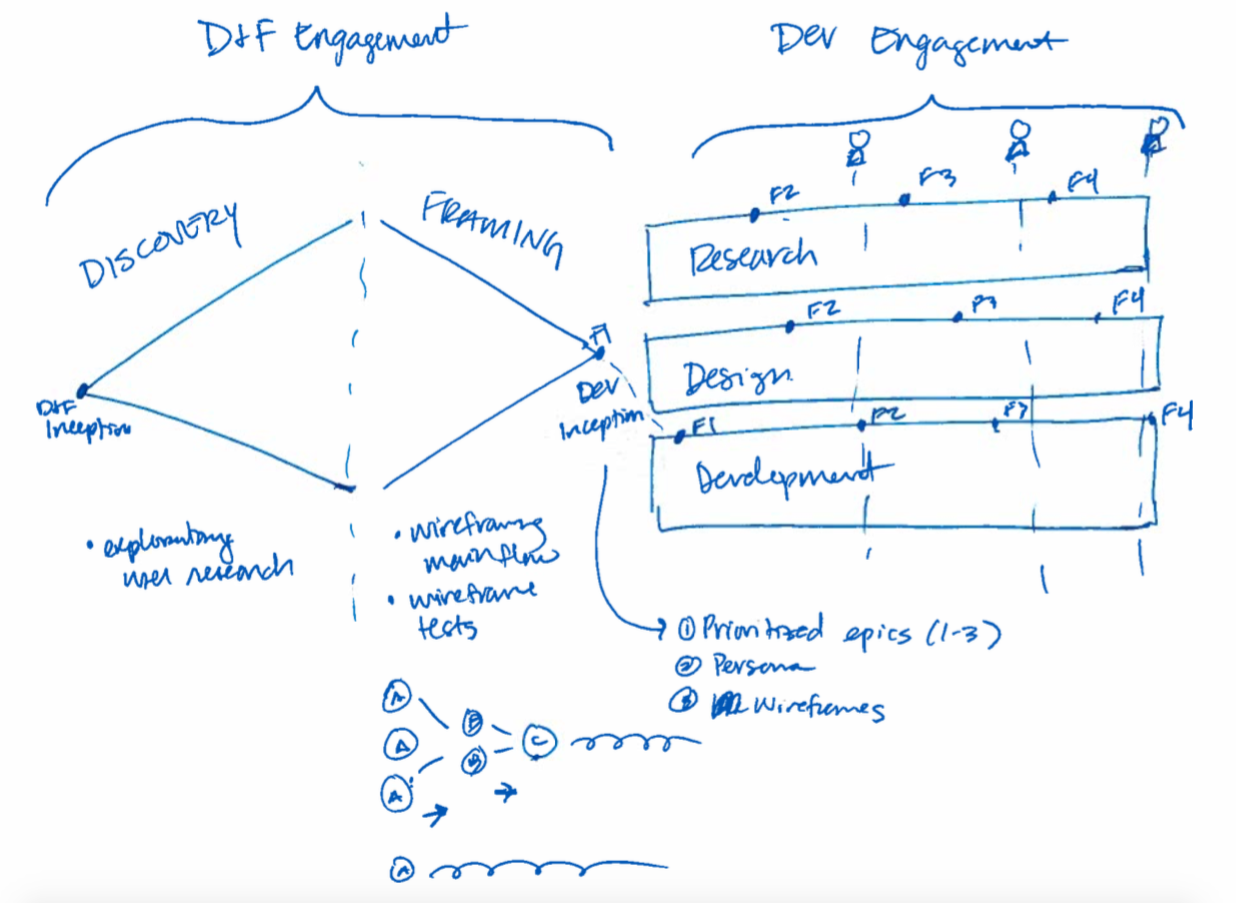
\includegraphics[width=6.5in]{interviews/drawings/2015_05_29.png}
\caption{\quotes{2015-05-29's drawing of a project work flow}}
\label{2015_05_29}
\end{figure}

\textbf{Interviewee:} Does it matter if there's a DNF first or...? 02:39

\textbf{Todd:} However you want it. Typical, ideal, however you want to draw it. 02:44

\textbf{Interviewee:} We actually show this to clients. We have this drawing here. 02:54

\textbf{Interviewee:} Most of the projects that I've been on start with the DNF. We'll call this DNF. 03:07

\textbf{Interviewee:} It's assuming the project has design in development going. This kind of, like, inception. 03:27

\textbf{Interviewee:} And this is dev inception. 03:32

\textbf{Interviewee:} This is your discovery, and framing. 03:50

\textbf{Interviewee:} Here in this area, we're sort of doing more exploratory research and sort of going wide trying to understand the users. That's something we do at the beginning of every project especially if the client doesn't know who their user is or they have ideas of who they are but it's not validated. 04:10

\textbf{Todd:} 	That's the discovery phase. 04:11

\textbf{Interviewee:} Yes. So, this is like exploratory user research. That's like interviews and maybe on site, shadowing people and things like that. And once we have a good idea of who they are, we start wire framing, maybe like the main flow and doing some wire frame tests like user research, that kind of thing and that's kind of within that, I think, we're kind of iterating as well. 04:45

\textbf{Interviewee:} I guess you can either start with one and iterate on that or you can start with many and narrow down. We've done both. So, when you start with many, you just- So, this is like your different As, research, then research to get to C. That makes sense? 05:10

\textbf{Todd:} It's like a portfolio of ideas? 05:14

\textbf{Interviewee:} Yes. I did it on my first project and it worked out really well and then from there you're kind of iterating on what you've come up with. 05:25

\textbf{Interviewee:} We came up with a couple, different nuance ways of doing something because they all seem good and they're like, two or three different features and we sort of combined them in different ways and then we took our insights from that and narrowed it down two versions, narrowed it down to one version. 05:46

\textbf{Interviewee:} I've also done it where you just start with A and you just iterate. I think both worked but this is fun to do. By the time we get to dev inception, we have prioritized epics. You have a develop persona. And you have wire frames. That's kind of the ideal for this point. At that point, development can start on say feature one and in the meantime, we'll start researching feature two. Then, we'll develop it. Then, feature three. So, it kind of goes like that. 06:37

\textbf{Todd:} Nice. 06:39

\textbf{Interviewee:} Maybe you have feature one here and then we'll go here. While they're doing that, we'll start on the next thing. So, on the next thing it flows down. I hate saying waterfall because I know it's the wrong kind. It's like a different kind of waterfall but it iterates in that way. So, we're like, \quotes{Oh, it's going in the cycle.} At any time, we're going to bring in users to test whatever we want. 07:09

\textbf{Todd:} You're drawing people. 07:12

\textbf{Interviewee:} Yes. These are users. At any given point, we can even do exploratory research. We can do wire frame or visual research or we can show them an actual prototype. 	It's kind of nice because you can, whenever you need people, whenever you're stuck on something, you don't have to wait for the right time to bring people in. 	It's just you can test anything at any given time.  07:34

\textbf{Todd:} Thank you. Have you seen a project that didn't quite fit this, what you've drawn here, this model? Or it was really different? 07:46

\textbf{Interviewee:} Yes. I was on a project. I was only on it for two weeks. It was just really quick enablement but there's basically no DNF. They came in with full visuals, full design. The problem is not a lot of it was validated. A lot of it was like, \quotes{Oh, the stakeholders thing. This looks nice.} 08:02

\textbf{Interviewee:} That was kind of different. As a PM, it was weird to write stories for full visual designs because I wasn't sure where to draw the line with the styling and things like that. We kind of had to feel it out. I think we stopped at colors and 	fonts. 	08:19

\textbf{Interviewee:} We did colors, fonts and a little bit of spacing for some other things but no animations, nothing like that. And that's also hard to convince the client, that maybe this isn't the right solution or things like that. I'm not sure how they got 	through without validation but it happens sometimes. 08:43

\textbf{Todd:} Do you think because it had such detailed mocks, they were married to their ideas? 08:49

\textbf{Interviewee:} I think so. It wasn't too hard, they're actually pretty open minded about stuff because they trust at our process. A lot of clients come in and like, \quotes{We trust you.} 08:58

\textbf{Interviewee:} For the most part, all the projects I've been on have been very flexible from that standpoint but I definitely felt bad for making the designer go through stuff. I don't think he minded but it's just a little bit harder to push back on things when they're not black and white and flexible. 09:21

\textbf{Todd:} Can you think of a different project that maybe didn't fit this mold in a different way? 09:27

\textbf{Interviewee:} Not out of the ones I've been on. They've mostly followed this. Like my first project followed this to a T. It was great. The second one just didn't have any discovery or framing. Right now, we kind of follow this as well. 09:51

\textbf{Todd:} I think given our sales process, we set this up for us. 09:56

\textbf{Interviewee:} You mean like non labs projects. 10:02

\textbf{Todd:} Just some labs. 10:02

\textbf{Interviewee:} 	Oh, just some labs. 10:03

\textbf{Todd:} Or in Pivotal. 10:06

\textbf{Interviewee:} Yeah. I haven't heard of any that- I think there are some enterprise projects that this doesn't quite work because there's an added QA layer. I haven't worked with a QA team but it just makes it harder to follow this because there's a QA layer that you have to go through in addition to acceptance. 10:28

\textbf{Todd:} In my current project, there's an approval process on designs and they want to see everything. You can't really do the features incrementally at least on design level. 10:40

\textbf{Interviewee:} That sucks. We have some design reviews. On most of the projects I've been on, we had weekly design reviews so nothing was a huge surprise to people. I guess I've just gotten lucky with the clients. They've been mostly receptive to our process. I hear horror stories about it but I haven't personally experienced any huge ones just yet. 11:09

\textbf{Todd:} As a PM, it feels like there's a lot that you juggle and manage. Is there one or two things that you remind yourself each day? What's the most important thing that you try to get right on a project? 11:26

\textbf{Interviewee:} If I'm working with a client, I always have to think about what I'm going to do with them. I think that's the biggest worry because I think any of the stuff I can do myself really quickly and I'll just remember things as they come up but I have to remember that I have to enable the client. 11:42

\textbf{Interviewee:} I have to be cognizant of what are we going to do today? What does the week look like? Not just the PM but I think PM in design especially during this period. It really helps to plan out the week just roughly and figure out okay, when are we doing research? What are some activities we should do? 12:01

\textbf{Interviewee:} There's some things you have to think about with the client from their perspective. Maybe they're not open to something. How do I convince them that this is the right way and try to put myself in their shoes and have empathy for them so I know how I can help turn them around to something that can work. Or help them come up with the idea. And I'm just like, \quotes{Oh you came up with this idea.} That kind of thing. 12:29

\textbf{Todd:} You mean you had the idea and you helped them realize the idea as well? Is that what you were saying? 12:35

\textbf{Interviewee:} Yes. We wanted them to go a certain way but they were like, \quotes{No we have to go this way.} How can we make them think that they came up with going this way. 12:43

\textbf{Todd:} It's like inception. You plant seeds. 12:45

\textbf{Interviewee:} Yes because they only listen to you so much. You tell people, \quotes{Trust me.} But they'll only trust you so much and then when they actually experience it, sometimes you just have to let people make a mistake and they feel that pain and they're like, \quotes{Oh okay. I will never do that again.} maybe not do that again maybe try this way. \quotes{Let's see what happens with that.} It's shows a different way of thinking. 13:12

\textbf{Todd:} What's it, for instance, on letting the client make a mistake and letting them feel that? 13:17

\textbf{Interviewee:} One time we had some clients who were very, very tight to us that are features and they call them core capabilities and very concrete and final and we kept trying to say, \quotes{Okay. These are assumptions.} They just didn't understand the word assumption. They're like, \quotes{No. We need to build these things.} 13:34

\textbf{Interviewee:} So, we did a couple of rounds of research because they weren't down for research. They never done that before and once they heard certain things, I think even though they heard certain things, their brain was still telling them they want these core capabilities. So, it's like they were, what is that called, like a confirmation bias or something like that or they're just like, \quotes{Oh yeah. That's what it means.} 13:53

\textbf{Interviewee:} And so, we did a synthesis and mapped out everything out and took their core capabilities and our main insights and tried to match them up. I think from there we could see that a lot of the insights didn't map to the core capabilities but it wasn't aggressive. We were all doing it together. 14:12

\textbf{Interviewee:} They were the ones making the mappings and saying like, \quotes{Oh. This moves down in priority. We didn't expect this to come up. Let's move on this first.} It took more time but it was nice that they came up with those conclusions on their own in a way or able to see that rather than us just telling them don't worry about this. Focus on the research. 14:37

\textbf{Interviewee:} You have to remember these clients come up with these things for months or years so they're very tied to them and to just rip them away from that is insensitive. I can empathize with them. You just have to have slowly validate or invalidate the stuff that they've been so closely tied to. 14:58

\textbf{Todd:} You described the client relationship and the parties you have with that. When you think about the development team, I'm biased, how to set them up for success, what's sort of things do you try and enable or set up for the team? 15:13

\textbf{Interviewee:} For the developers specifically? 15:15

\textbf{Todd:} PM. They're trying to make everything hum than what you imagine. 15:19

\textbf{Interviewee:} I keep communication really open. Before I start a project, if I can I like to talk to whoever is the anchor or the designer in the team and just get a feel for how they work with the PM because everybody's a bit different. 15:36

\textbf{Interviewee:} Big things that they would expect from a PM that I might miss or something like that and just try to get a feel for how they work with other people and obviously retro is great for a lot of that stuff. 15:50

\textbf{Interviewee:} Sometimes, we've had retros where we just talk about- because I think in front of the client you have to have a united front. And for the most part, in my experience, it's been great but if there are any disagreements or any problems, you don't want to bring up in front of the client it's really nice to have a pivotal retro. 16:09

\textbf{Todd:} How frequently might you have one of those? 16:12

\textbf{Interviewee:} Depending on how bad the project is. Once a week, maybe. Maybe once every other week. I don't know. 16:19

\textbf{Todd:} On top of the normal retro? 16:21

\textbf{Interviewee:} On top of. We have the normal retro usually and if we were at a point where we're feeling disconnected, we might have one. So, it kind of depends. I've never been in a situation where I needed one weekly. Although I've heard of those, really stressful ones. 16:39

\textbf{Todd:} Think of one of the worst projects you've been on, what's one thing you did to try and right it and get it back on track? 16:47

\textbf{Interviewee:} I haven't had any that were horrible. I think there was some bad times in my first project because the client wasn't committing to certain things. Once they went back to their own office. 17:10

\textbf{Interviewee:} We're working remotely and they were just being pulled into meetings. I think I was a little harsh. I don't know. I was just like, \quotes{Hey, the backlogs' drying, designing guys need to do stuff.} Because the devs were running out of things to do. They're just like, \quotes{What do we do?} 17:27

\textbf{Interviewee:} I tried to find other things that didn't require design to be prioritized. For that, I needed some help from the anchor because I don't have a formal technical background. 17:39

\textbf{Interviewee:} A lot of times I'll just ask. I'm like, \quotes{Hey, teach me this stuff.} Sometimes I'll have the devs say in stand-up that the backlogs' dry because I find the people listen to devs more than PMs or they take it more seriously. So, I'm just like, \quotes{Okay. You just say it.} I can say it 10 times but as soon as the devs say it, they're like, \quotes{Oh my god. [Interviewee] We're freaking out.} And I was just like, \quotes{Yes. I was freaking out two weeks ago.} 18:09

\textbf{Interviewee:} Sometimes you just have to be a little harsh. Just be like, \quotes{I know you have a meeting but we really need to move on this right now.} 18:21

\textbf{Interviewee:} I also paired with devs and designers which I think helped bring the team a little bit closer. The client PM was there half the time but I encourage him to pair sometimes. I really like cross functional pairing. 18:35

\textbf{Todd:} When you pair with dev, do you work on a story with the dev?18:39

\textbf{Interviewee:} Yes. I do whatever they're doing and I'm not necessarily coding from scratch but I know enough to recognize where things go. We'll type this in here or I might watch them do something then I'll do it. 18:52

\textbf{Interviewee:} A lot of it is discussion and asking questions. Like on this particular time, I had been on a project longer than the dev and so she wasn't sure where everything lived and I was like, \quotes{I think that data is over here. Can we do control+F for this keyboard} We're trying to figure out why something didn't work and I had a little more context so I was able to talk about it and she's like, \quotes{Oh. I know where that is. Let's try doing that type of thing.} It was a lot of back and forth. 19:22

\textbf{Todd:} Nice. I have not experienced that. 19:25

\textbf{Interviewee:} Yes. It's really fun. I love pairing with devs. It's also really intimidating. If you're at the helm of a spaceship or something and you're just like, \quotes{Oh my god.} but it's pretty fun. Everybody I've paired with has been really nice and patient and they like teaching. I was like, \quotes{Cool. Teach me.} 19:41

\textbf{Todd:} Pairing with designers makes sense to me, I think. 19:48

\textbf{Interviewee:} Yes. Again, it's a lot of discussion. Maybe we should put this here instead of there. I didn't know how to use Illustrator before but know I can poke around and use it. So, sometimes I get to do some stuff too. 20:01

\textbf{Todd:} That's fantastic. 20:03

\textbf{Interviewee:} Yes, it's really fun. 20:04

\textbf{Todd:} So, as a dev, sometimes I think about non functional requirement or they're called quality attributes. How do you handle those? As a PM, how does that work for you? Do you think about them? 20:19

\textbf{Interviewee:} You mean like visual design, thing like that? 20:23

\textbf{Todd:} Things like maybe performance or security or liability of the system. We call them ilities. There's like 20 of them that might show up in a project. 20:31

\textbf{Interviewee:} Yes. I think about them a little bit, honestly, in my experience here, at least. It's usually the devs or the client PM who is bringing it up. I should think about it more probably but when I think about MVP, it's like user mode but I think those get prioritized. 20:49

\textbf{Interviewee:} We just feel it out and honestly it's more of the client PM's decision and because they know the product better. If they're really, really lost, we'll try to make the most informed decision with them. 21:02

\textbf{Interviewee:} If we're about to launch or we want to do an initial release and obviously some of that stuff has to go forward. If some things, like really unknown or there's high risk, sometimes we try to write a story and just get that one story out there because that drives out a lot of the risk and drives out a lot of things that we might not know. 21:21

\textbf{Todd:} Trying to reduce risk makes sense to me. In my experience at Pivotal, I've not seen any stories about performance or things like that. That makes sense at some level because stories are about features. They're not about attributes of the system and I haven't seen how anyone here handles that. I'm curious... 21:44

\textbf{Interviewee:} I try to write all stories from a user perspective so I might say something like, \quotes{I want the spatial load faster because it's taking a really long time right now.} That kind of thing and so I know some places have requirements of loads in two seconds and things like that. 22:01

\textbf{Interviewee:} I haven't quite gotten down to that level but I'll still write it from a user perspective and if I have an idea of what might be slowing something down for example, I'll put it in there. \quotes{Oh, we have a page full of SVGs maybe we can convert them on to PNGs or something like that.} I try not to be too prescriptive because that's just not my place. 22:24

\textbf{Todd:} Good. 22:27

\textbf{Interviewee:} I try to handle them from the user perspective as much as possible. 22:30

\textbf{Todd:} I have created a little model for stories. This is now called described or something. Defined. 22:44

\textbf{Todd:} From your perspective, this is a flow of stories, give me feedback for me on those. 22:53

\textbf{Interviewee:} Named is just identifying the story. Once you flush them out and written them and they've been through pre-IPM and they're estimated, they're started, blocked. I usually don't go back and estimate. So, it's like this. 23:12

\textbf{Todd:} It could happen. 23:13

\textbf{Interviewee:} I usually don't do this. I guess it depends on what's happening here. I haven't re-estimated a story unless we pointed it five weeks past and then it comes up in the backlog, we might revisit it and say, \quotes{Okay. Do we still think it re-points?.} 23:35

\textbf{Todd:} Well, we try not to re-point. I agree with that. 23:37

\textbf{Interviewee:} I haven't done that. Started, finished, delivered, accepted. 23:42

\textbf{Interviewee:} Delivered. Checked in. This would go back to - Oh, you have that here. Delivered. So, when will it go from delivered to started?  23:56

\textbf{Todd:} The irony is this actually comes form tracker data, this graph. I went through a ton of project and watched all the transitions of every story and there was a story from delivered to started. 24:08

\textbf{Interviewee:} Maybe they delivered on accident? That sometimes happens. Or was it delivered on purpose? 24:14

\textbf{Todd:} I think what happens there is you deliver it and then you realize there's more work to be done. 24:19

\textbf{Interviewee:} Oh, so the dev will go back and... 24:20

\textbf{Todd:} Say, \quotes{Oops. We're not done.} 24:23

\textbf{Interviewee:} Okay. 24:24

\textbf{Todd:} Or someone will walk by and say, \quotes{That's not done. You didn't do X.} 24:28

\textbf{Interviewee:} Just like  before the PM hits something, they'll say, \quotes{Hey, you guys, forgot this.} 24:32

\textbf{Todd:} It's kind of like the rejection where the PM didn't reject it. 24:34

\textbf{Interviewee:} That makes sense. I've done that before. Finish, delivered, accepted. 24:40

\textbf{Todd:} That has happened, believe it or not. 24:47

\textbf{Interviewee:} Really? 24:48

\textbf{Todd:} I agree with you, the ideal is that would not happen. My point in showing this is to actually help you make sense of what I'm about to show you next. This is my view of stories. 24:56

\textbf{Interviewee:} I've been trying to create a checklist items for each state that the story could go in. I just wanted you to look at this list and see if you have any... 25:06

\textbf{Interviewee:} The idea is, for something to be named how do you know it's named or not and these would have to happen for each state. If this is not clear, ask questions and I'll try and clarify. 25:19

\textbf{Interviewee:} Okay. I think this is like an either/or. It could be prioritized or it could not be. Can we write down? 25:34

\textbf{Todd:} Sure. Whatever you want. 25:36

\textbf{Interviewee:} Defined. Feature is prioritized. I think this can also be either/or. 25:45

\textbf{Interviewee:} I usually don't prioritize until - I'll have a rough priority but I'll wait until they're all flushed out. Sometimes in pre-IPM even they're not fully prioritized by this time. Usually after they're estimated, usually they're prioritized but sometimes after they estimate, I'll rethink some things. 26:13

\textbf{Interviewee:} If they're not fully prioritized, that's okay. 26:16

\textbf{Interviewee:} Story describes clear acceptance criteria. That makes sense. That makes sense. 26:22

\textbf{Interviewee:} Story only describes user interaction with system. Yes. I think some people do this. I really like to do this. Oh, ideal PM. 26:33

\textbf{Todd:} That's your ideal. 26:34

\textbf{Interviewee:} Yes. 26:35

\textbf{Todd:} It doesn't have to happen. 26:35

\textbf{Interviewee:} Yes. Business value is clear. Yes. I'd say, relevant. Did you already write that? 26:59

\textbf{Todd:} No. I did not. 26:59

\textbf{Interviewee:} I try to attach design to every story. I try not to write a story before a design is done and that works out really well. And that's kind of the ideal. 27:09

\textbf{Interviewee:} Estimated. Feature is estimated. Nothing blocks developers from working on the story. Yes. I would even make this required. 27:24

\textbf{Todd:} I've estimated stories that were blocked that's why it's ideal. So you feel strongly about that. 27:34

\textbf{Interviewee:} If it's blocked, I don't. 27:36

\textbf{Todd:} Why do you estimate it? 27:37

\textbf{Interviewee:} It's not going to be accurate. I guess there are some stories where the devs are kind of like, \quotes{Well, I've never worked with that before.} If something's not defined or this is clearly blocked then I'll probably be like, \quotes{Okay. We'll just wait.} 28:00

\textbf{Todd:} Would you say it would be okay to estimate if you're trying to figure out when the end of the project is going to be even though things might be blocked? 28:06

\textbf{Interviewee:} Yes. I can see doing that. I've heard of that. I haven't don that on a project yet but I know they've been pointing  parties where people do small, medium, large type of thing or really rough pointing estimates. I think that's fine but for an IPM when you're going to work on something ideally, it's not blocked. Started. Yes. Blocked. It depends to you. Yes. I think that makes sense. I can't speak to these two. 28:37

\textbf{Todd:} You've paired on code so you might have more of an opinion on that than other PMs. 28:45

\textbf{Interviewee:} I agree with it. It makes sense. It was funny, I was pairing with somebody and we were working on an iOS project but it also involved JAVA and so we had, was it C\# or not C\#, what is it? 28:58

\textbf{Todd:} Objective C. 28:59

\textbf{Interviewee:} I guess she's more familiar with Objective C and not JAVA. She's kind of like, \quotes{Oh. I don't know Java that much.} She was like, \quotes{It all looks the same to me.} It looks equally confusing. 29:15

\textbf{Interviewee:} Units test pass, makes sense. Acceptance passes. What is the difference between a unit test and acceptance test? 29:28

\textbf{Todd:} Unit test are the very low level. They test one thing in isolation. Acceptance test, they're more PM level. Does the feature do what it's supposed to do? Does the story work? 29:42

\textbf{Interviewee:} So, the devs will do an acceptance test. 29:47

\textbf{Todd:} Sometimes they have them sometimes they don't it depends on the project so I'll probably put ideal or optional on there as well. 29:51

\textbf{Interviewee:} Is that something actually written or is that more of like the devs going through what they acceptance criteria says? 30:02

\textbf{Todd:} It depends on the project. Some of them we will write acceptance test. 30:08

\textbf{Interviewee:} Code reviewed prior to commit. Changes reviewed prior to commit. That makes sense. Delivered. Yes. PM updated the acceptance criteria because they were not clear. 30:28

\textbf{Todd:} You're going to fill out some of these. Go ahead keep going. 30:32

\textbf{Interviewee:} I do some of these things. Additional requirements that need to be implemented. The PM changed the requirements and the codes need rework. This shouldn't happen. This shouldn't happen. This shouldn't happen. 30:50

\textbf{Todd:} I completely agree with you. 30:52

\textbf{Interviewee:} If the PM changes their requirements, if it's small, sometimes, I'll say, \quotes{I meant this but I forgot to put it in.} If it's really tiny, they're like, \quotes{It's okay we'll just do it.} I'm like, \quotes{Okay. Thanks} 31:03

\textbf{Todd:} Why write another story. 31:03

\textbf{Interviewee:} Yes. And I'll just put a comment. I'll say, \quotes{It works but I forgot to add this.} So, devs rejecting so you can add this thing or something like that. But if it's something big, I'll be like, \quotes{Sorry, I forgot that.} And I'll just write another story. I'll be like, \quotes{Let me just write another story.} 31:23

\textbf{Interviewee:} Sometimes I'll write a bug and I don't have a clear criteria when it's a bug and when it's an extra feature but in the moment it makes sense. I just can't think what I used to decide it's a bug or not. 31:38

\textbf{Todd:} I know what I use. 31:43

\textbf{Interviewee:} One time, we were building something where you can adjust the quantity in a card and we were like, \quotes{It has to be an integer. it can't be zero.} And we were able to add zero and we were like, \quotes{We shouldn't be able to add zero.} That was a rejection but the fix they made, it had to be applied to this other scenario that wasn't covered in the story. But since they did it for one, \quotes{Okay. Let's just create a bug for it.} Because it was treated as a bug in the other scenario so it's kind of like a weird scenario. 32:21

\textbf{Todd:} For me, the black and white description is, if the story says it should do something and the code doesn't, that's a bug. If a story doesn't describe that condition, then it's a new feature. 32:32

\textbf{Interviewee:} Yes. 32:34

\textbf{Todd:} There's probably a gray area. 32:36

\textbf{Interviewee:} Yes. There are some gray areas where you decide should I reject it or should I write a bug type of thing. I think, definitely, in that first scenario, it's either reject a bug or usually that would just be a rejection because it says it should do this but it doesn't. 32:49

\textbf{Interviewee:} Anything additional should be another story but sometimes I do a bug instead of a rejection for some reason and I think it's for little things. PM updated the acceptance criteria because they're not clear. That sometimes happens. If it's small. So, I'll say, if it's small. And sometimes when I reject something if it's really nitpicky, I'll put nit. Do you guys do that? 33:18

\textbf{Todd:} What does that mean for you? 33:21

\textbf{Interviewee:} I don't know. A dev told me to do that one. I think it stands for nitpicky or nitpicking. I don't know. Sometimes, I'll be like the word is off or something. Technically it can go out but it should have this other word or the color is a little bit wrong and I'm just this works perfectly but I'll say it, nit. 33:44

\textbf{Todd:} So, in the comments of the story, you will put nit:fix this. 33:51

\textbf{Interviewee:} Yes. I feel it's a little nicer. I don't know. It's just like nothing's wrong, it's just the mock has this and it's a UI type of thing. A Dev told me to do that once. I was like, \quotes{Okay. I feel better about doing that because I feel bad rejecting stories that are technically work but just have a weird...} 34:10

\textbf{Todd:} I think I've seen one PM not accept it and put a comment on it,  which notifies people and then they would accept it once it's fixed. But rejection is probably the right flow. 34:22

\textbf{Interviewee:} Yes. If it's not rejected, you're not going to see it. As a dev, I would imagine. QA manager added new requirements. This should happen. I just think that's so silly but I guess some big companies have a QA process but they should not add new requirements. They should be bugs features and then... 34:55

\textbf{Interviewee:} I've had QA say, \quotes{Oh, this doesn't work.} or \quotes{This has this one case it won't take a credit card after 2049.} I was just like, \quotes{Okay. Let's write a bug} but I just put at the bottom backlog. We'll put them in the backlog but the PM will prioritize it as they prioritize everything else. That shouldn't lead to a rejection ever. 35:17

\textbf{Todd:} Given everything that we talked about in this conversation, is there anything else that you think would be relevant? Maybe questions I should ask? 35:26

\textbf{Interviewee:} What is your objective? What stuff do you want to know? 35:31

\textbf{Todd:} I should have a clear answer to that question. I think at this point, I'm really curious how what we do differs from what Kent Beck described 15 years ago. We've done a lot of really neat things and so I've been really interested in that. And I have a question I'd prefer to ask without leading it. Why do we call an IPM an iteration planning meeting? 36:10

\textbf{Interviewee:} Versus? 36:13

\textbf{Todd:} Why do we call it that? There's things that we do in the meeting and does the name describe what we do in the meeting? What's the purpose of an IPM? 36:27

\textbf{Interviewee:} It's so the team is aligned in what we're going to be doing for the next iteration or the next week. I guess, sometimes, the things that you point in IPM don't always line up to what you're going to be working on in a week. Sometimes, we'll end up pointing a lot of things. I think it's a good way. I think ideally, it is supposed to spell what the team is going to be working on for the next week or the next iteration. 36:54

\textbf{Interviewee:} So, you know you have immediate contact. You just pointed it. You know exactly what's happening. There's not a lot of time between for you to forget. Most of the time it happens or at least you'll start working on some of the things you pointed on that week but I think also it's a good rhythm setter for the team like you meet every week and you feel like you have this check in. You're always connected. You have frequent connections with dev and PM and design. Because I think PM and design can be off. We're usually ahead, design especially but PM, kind of split but we have fear what's going on right now and also be two weeks ahead and so I feel like this helps bridge the gap between what's going on in the design world and the dev world and having those check ins really helps 37:48

\textbf{Todd:} For me, it's like weekly estimation meeting. About six months into my career here, I realized that, for me, in my perspective there is no iteration. We do retros on Fridays because Mondays we don't remember what we did last week. We do weekly estimation meetings somewhere in the middle because we need to have enough work. The worst thing that could probably happen is I have six devs with nothing to do. So, we need to make sure that there's enough of a backlog for them. I was on a project where I had no idea that iteration started on Tuesday. And that was the clue for me. What? Are there iterations starting on Tuesday? I had no idea. 38:28

\textbf{Interviewee:} So, what do iterations mean for you then? 38:31

\textbf{Todd:} I think there is no spoon. I think it's a very kanban-like the work flows through us. The team isn't committing to a scrum that says, next week we're going to deliver these three features. 38:44

\textbf{Interviewee:} Yes. I can see what you mean by that. I feel that way, too, sometimes. 38:49

\textbf{Todd:} I think that's great. We show up and we do where the work is needed. 38:54

\textbf{Interviewee:} Yes. 38:56

\textbf{Todd:} So, halfway through a week something in the universe completely changes, we respond to it and start adapting to it. It's not like there's this ready plan. On Friday, we're going to launch this feature. We can't do that. In the original definition of XP, the team was committing to where they will be each week. 39:16

\textbf{Interviewee:} I didn't know that. 39:17

\textbf{Todd:} Yes. 39:18

\textbf{Interviewee:} I had no idea. I thought XP was totally. 39:21

\textbf{Todd:} And you couldn't change what the team would do that week? It was inflexible. 39:24

\textbf{Interviewee:} That's against everything that we do. I actually didn't know that and I read the XP book. 39:30

\textbf{Todd:} If the PM changed what they did during the first week, there was a contract violation between you and the team. 39:36

\textbf{Interviewee:} That's so crazy. I need to go re-read that book or something because I totally have been telling clients XP is flexible. 39:41

\textbf{Todd:} and..with XP..what we do here. That's really interesting. 39:45

\textbf{Interviewee:} Yes. That's kind of how I see it. I think, if anything, it gives a team a rhythm. I think retros help us sort of figure out what didn't go well during the week. What we need to change so it's not at some arbitrary point somebody might say, \quotes{This isn't working. Let's try to figure out how to change it} There's a forced check in so anything that you think you had a problem with this week, you know we'll come up at least every week and then you can do something to make the next week better. I think, work flow wise, maybe we're not doing things iteratively but team-cadence wise, we have iterations of like, Okay. Let's take an arbitrary piece of time. A day's too short, a month is too long. So, let's do a week. Just make sure there are teams running smoothly every week. I think it serves that purpose maybe more than the actual delivery and execution. It's more about the team spirit, I guess. 40:59

\textbf{Todd:} I think what I'm hearing you say is, your view of the word iteration might be different than mine and so you're happy to call in IPM because, for you, it's this weekly rhythm that's maybe artificial because of weekends. If there were no weekends, we might have a different rhythm or something 41:20

\textbf{Interviewee:} Yes. 41:21

\textbf{Todd:} It wouldn't be healthy 41:22

\textbf{Interviewee:} Yes. I think it's like a force check in because we were just to do things. We think about things in terms of time and so if we didn't have a time marker I think we would just get very confused and we would get very lost in what we're doing. 41:40

\textbf{Interviewee:} And even new devs are estimating stories, they still want to estimate in terms of time. We're always thinking in terms of time because that's how the world works in a way and so I think having that time marker helps us keep things in check versus if we just let them run on forever. 41:58

\textbf{Interviewee:} So, yes. I guess I think about iterations. I haven't thought about this deeply before but I guess me, for iterations, it's more like the team rhythm and team cadence versus the actual execution of things. 42:09

\textbf{Todd:} Yes. Okay. 42:11

\textbf{Interviewee:} I guess iteration in context of how we use it here. 42:14

\textbf{Todd:} That's very helpful for me. I'll have to deep think on it some more. 42:18

\textbf{Interviewee:} Building iteratively I think it means something else. Like what I was saying in the beginning, you just start with the first layer and the second layer. That's a little bit different than what I'm thinking in terms of team iteration if that makes sense. 42:31

\textbf{Todd:} It does. I don't have anything else. Is there anything else you wanted to share or anything you're not telling me? 42:40

\textbf{Interviewee:} I don't think so. I've worked in waterfall before so this is like a huge breath of fresh air. I think it's much healthier. I think the ideal of what this is supposed to be is good but it's not always applicable especially with enterprises, for example. We've definitely had to bend a little bit more to work with enterprises because it's just not the solution for everybody. You have to cater a little bit to different types of organizations. 43:19

\textbf{Todd:} I forgot about demographics. How long have you been at Pivotal? 43:21

\textbf{Interviewee:} I've been here almost a year. I started in August. 43:25

\textbf{Todd:} Just in terms of your career, when did you graduate from college? 43:31

\textbf{Interviewee:} 2010. 43:32

\textbf{Todd:} Great. That's it. 43:33

\textbf{Interviewee:} Okay. Cool. 43:34

\textbf{Todd:} Thank you. 43:34

\textbf{Interviewee:} Yes. Thank you. This was fun. 43:36





\bibliographystyle{IEEEtran}
\bibliography{bibliography}

\backmatter


\end{document}